\documentclass[12pt]{report}
\usepackage[utf8]{inputenc}
\usepackage[spanish]{babel}
\usepackage[T1]{fontenc}
\usepackage{geometry}
\geometry{a4paper, margin=3cm}

\usepackage{setspace}
\onehalfspacing
\usepackage{graphicx}
\usepackage{float}
\usepackage{caption}
\usepackage{subcaption}
\usepackage{amsmath, amssymb}
\usepackage{array}
\usepackage{tabularx}
\usepackage{multirow}
\usepackage{booktabs}
\usepackage[table,xcdraw]{xcolor}
\usepackage[most]{tcolorbox}
\usepackage{verbatim}
\usepackage{placeins}
\usepackage{longtable}

% ####################################
\usepackage[absolute,overlay]{textpos}
\usepackage{lmodern}
\usepackage{iflang}
\usepackage{xspace}

\usepackage{titlesec}
\usepackage{eso-pic}

% ####################################
% Citas
\usepackage[round]{natbib}


% Hyperlinks: siempre debe ir antes de acronym
\usepackage{hyperref}

% Encabezados y pies de página personalizados
\usepackage{fancyhdr}

% Acrónimos (Después de hyperref)
\usepackage[printonlyused]{acronym}


% #### Nuevos paquetes #######
%
\usepackage{enumitem}
\usepackage{minted}
\usepackage{tikz}
\usetikzlibrary{calc}


\renewcommand{\headrulewidth}{0pt} % Sin línea en el encabezado
\renewcommand{\footrulewidth}{0pt} % Sin línea en el pie

% Configuración del banner inferior desde la página 1
% Ajustes de posición en puntos (1pt ≈ 1 pixel a 72 DPI)
\newcommand{\bannerHeight}{68.16pt} % 2.4cm = 68.16pt
\newcommand{\bannerXOffset}{0pt} % Desplazamiento horizontal del banner
\newcommand{\bannerYOffset}{0pt} % Desplazamiento vertical del banner
\newcommand{\pageNumXOffset}{28.35pt} % 1cm = 28.35pt - posición X del número
\newcommand{\pageNumYOffset}{35.05pt} % 3cm = 85.05pt - posición Y del número

% Marcador para la sección de Siglas
\newcommand{\siglaref}{\hyperref[cap:siglas]{\nameref{cap:siglas}}}

% ################## DEFINICIÓN DE SIGLAS ######################
\newcommand{\HTC}{\hyperref[cap:siglas]{HTC}\xspace}




% ##############################################################

% Comando para capítulos SIN numeración de página (páginas especiales)
\newcommand{\ChapterImageEmpty}[3][]{%
	\cleardoublepage
	\thispagestyle{fancy}%
	\refstepcounter{chapter}%
	\AddToShipoutPictureBG*{%
		\begin{tikzpicture}[remember picture,overlay]
			% Imagen de fondo al ancho de la página
			\node[inner sep=0pt, anchor=north west] at (current page.north west)
			{\includegraphics[width=\paperwidth]{#3}};
			% Caja blanca que se adapta al ancho del texto
			\node[
				anchor=north west,
				xshift=1.5cm, yshift=-1.0cm,
				text=black,
				fill=white, fill opacity=0.8,
				rounded corners=6pt,
				inner xsep=10pt, inner ysep=6pt
			] at (current page.north west)
			{\Large\bfseries \thechapter\quad #2\strut};
		\end{tikzpicture}
	}%
}

% Comando para secciones preliminares (sin numeración pero en índice)
\newcommand{\ChapterImagePrelim}[3][]{%
	\cleardoublepage%
	\phantomsection%
	\addcontentsline{toc}{chapter}{#2}%
	\AddToShipoutPictureBG*{%
		\begin{tikzpicture}[remember picture,overlay]
			% Imagen de fondo al ancho de la página
			\node[inner sep=0pt, anchor=north west] at (current page.north west)
			{\includegraphics[width=\paperwidth]{#3}};
			% Caja blanca que se adapta al ancho del texto
			\node[
				anchor=north west,
				xshift=1.5cm, yshift=-1.0cm,
				text=black,
				fill=white, fill opacity=0.8,
				rounded corners=6pt,
				inner xsep=10pt, inner ysep=6pt
			] at (current page.north west)
			{\Large\bfseries #2\strut};
		\end{tikzpicture}
	}%
}

% Comando para capítulos CON numeración de página (capítulos normales)
\newcommand{\ChapterImageStar}[3][]{%
	\cleardoublepage%
	\refstepcounter{chapter}%
	\addcontentsline{toc}{chapter}{\protect\numberline{\thechapter}#2}%
	\AddToShipoutPictureBG*{%
		\begin{tikzpicture}[remember picture,overlay]
			% Imagen de fondo al ancho de la página
			\node[inner sep=0pt, anchor=north west] at (current page.north west)
			{\includegraphics[width=\paperwidth]{#3}};
			% Caja blanca que se adapta al ancho del texto
			\node[
				anchor=north west,
				xshift=1.5cm, yshift=-1.0cm,
				text=black,
				fill=white, fill opacity=0.8,
				rounded corners=6pt,
				inner xsep=10pt, inner ysep=6pt
			] at (current page.north west)
			{\Large\bfseries \thechapter\quad #2\strut};
		\end{tikzpicture}
	}%
}

\newcommand\BackgroundPic{%
	\put(-25,-2){%
		\parbox[b][\paperheight]{\paperwidth}{%
			\vfill
			\centering
			
\includegraphics[scale=1,height=\paperheight]{./images/fondo-anteportada.png}%
			\vfill
		}}}

\newcommand\PortadaPic{%
	\put(0,0){%
		\parbox[b][\paperheight]{\paperwidth}{%
			\vfill
			\centering
			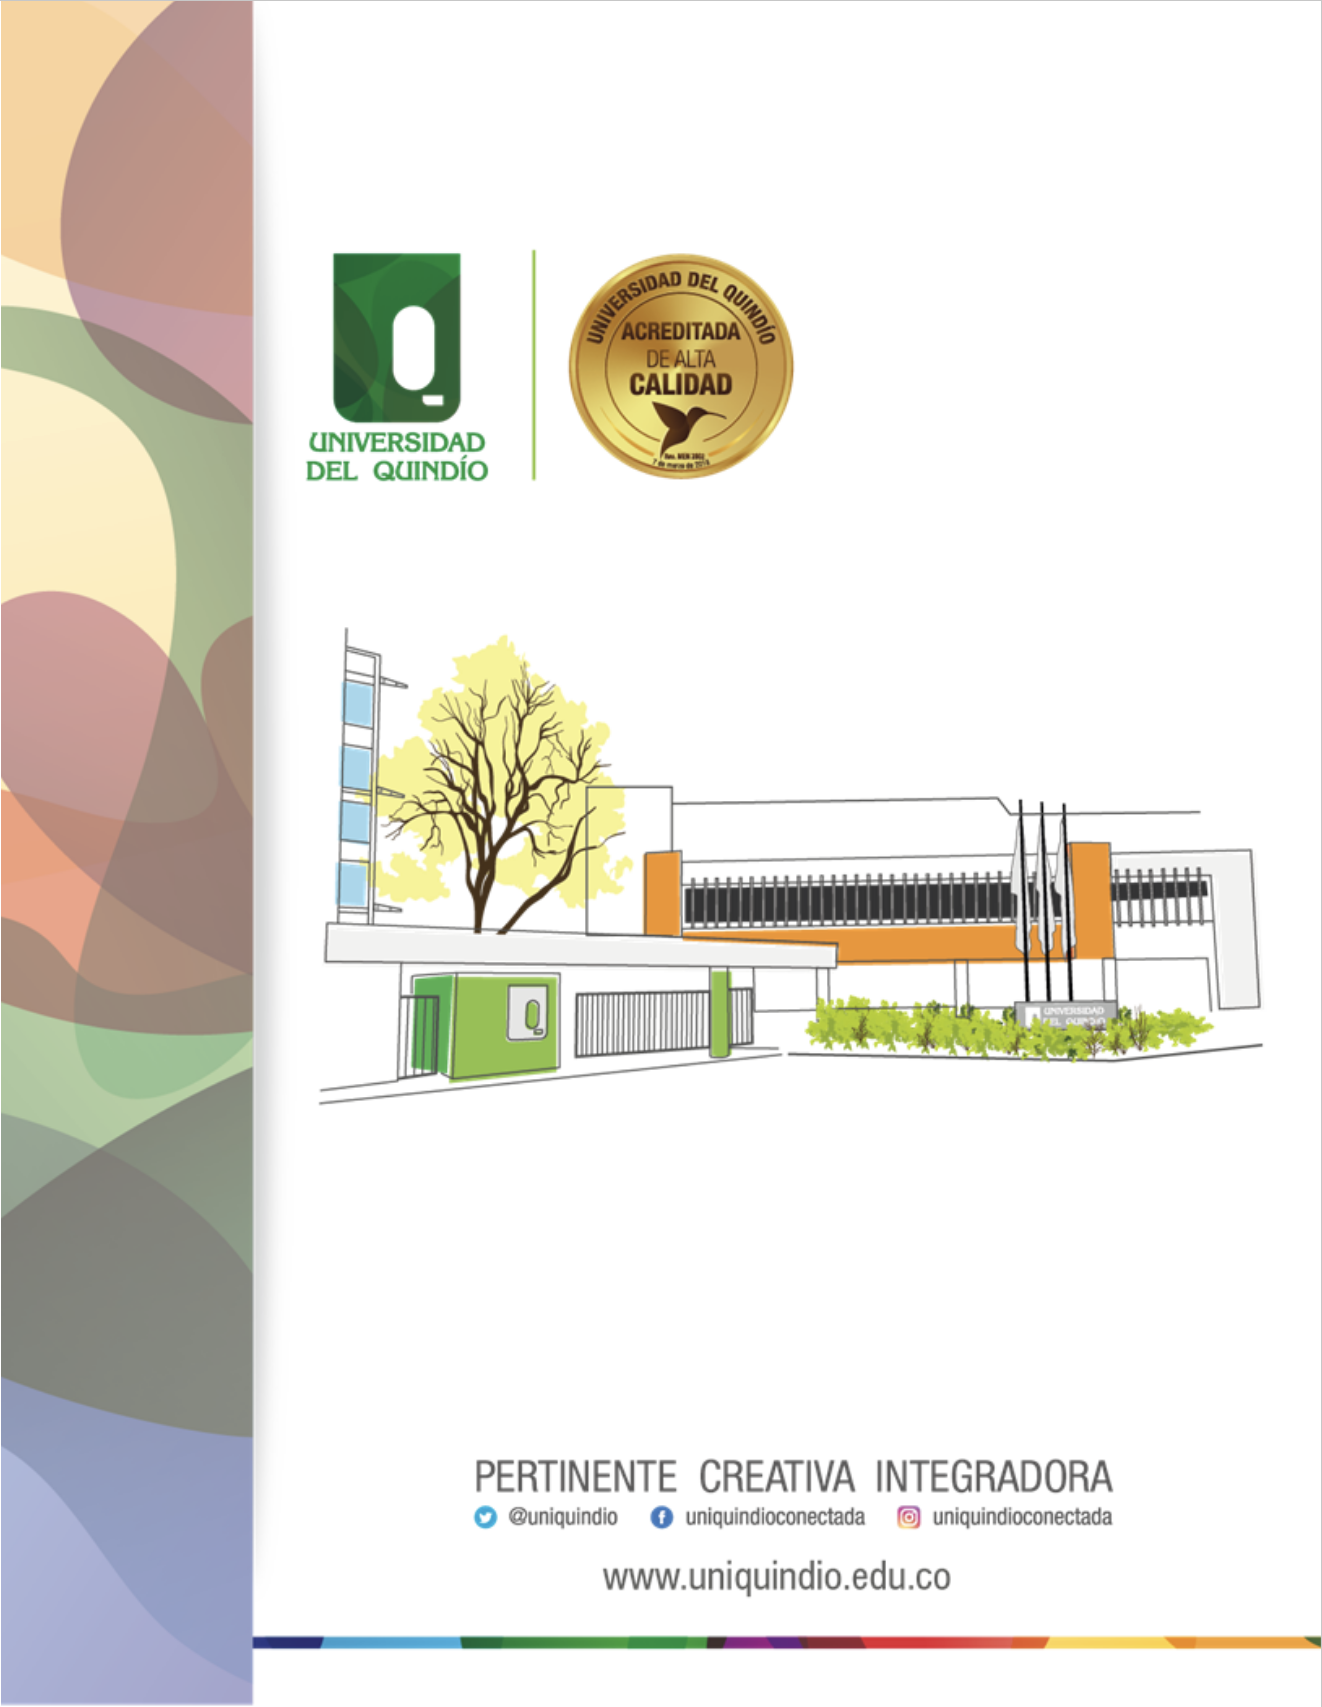
\includegraphics[width=\paperwidth,height=\paperheight]{images/portada.png}%
			\vfill
		}}}




\begin{document}


%\AddToShipoutPicture*{\BackgroundPic}
\begin{titlepage}
    \thispagestyle{empty} % quita encabezados/pies de página

    % Aquí sí usamos TikZ correctamente
    \begin{tikzpicture}[remember picture,overlay]
        \node[anchor=west] at ([xshift=6cm,yshift=-5cm]current page.north west)
            {\LARGE\bfseries \mytitlea};
    \end{tikzpicture}
    \begin{tikzpicture}[remember picture,overlay]
        \node[anchor=west] at ([xshift=3.5cm,yshift=-5.7cm]current page.north west)
            {\LARGE\bfseries \mytitleb};
    \end{tikzpicture}
    \begin{tikzpicture}[remember picture,overlay]
        \node[anchor=west] at ([xshift=2.8cm,yshift=-6.4cm]current page.north west)
            {\LARGE\bfseries \mytitlec};
    \end{tikzpicture}
    \begin{tikzpicture}[remember picture,overlay]
        \node[anchor=west] at ([xshift=4.5cm,yshift=-7.1cm]current page.north west)
            {\LARGE\bfseries \mytitled};
    \end{tikzpicture}

    \begin{tikzpicture}[remember picture,overlay]
        \node[anchor=west] at ([xshift=8cm,yshift=-19cm]current page.north west)
            {\normalsize \myname };
    \end{tikzpicture}
    \begin{tikzpicture}[remember picture,overlay]
        \node[anchor=west] at ([xshift=9cm,yshift=-19.5cm]current page.north west)
            {\small Cc: \matricle};
    \end{tikzpicture}

   \begin{tikzpicture}[remember picture,overlay] 
        \node[anchor=west] at ([xshift=8cm,yshift=-21cm]current page.north west)
            {\normalsize \mynameb};
    \end{tikzpicture}
    
    \begin{tikzpicture}[remember picture,overlay]
        \node[anchor=west] at ([xshift=9cm,yshift=-21.5cm]current page.north west)
            {\small Cc: \matricleb};
    \end{tikzpicture}
    \clearpage % fuerza nueva página después
\end{titlepage}
\ClearShipoutPicture
%\AddToShipoutPicture*{\PortadaPic} % agrega la imagen de fondo
\begin{titlepage}
	\thispagestyle{empty} % sin encabezado ni pie

	% Usamos TikZ para colocar texto en posiciones absolutas
	\begin{tikzpicture}[remember picture,overlay]

		% Logo en (x,y) desde esquina superior izquierda

		% Título en coordenadas absolutas


		% Tipo de trabajo
		\node[anchor=west] at ([xshift=14cm,yshift=-6.5cm]current page.north west)
		{\Large \mytype};


		% Revisor y asesor
		\node[anchor=west] at ([xshift=8cm,yshift=-21.5cm]current page.north west)
		{\begin{tabular}{rl}
				Revisor:  & \reviewerone \\
				Director: & \advisor
			\end{tabular}};

		% Fecha
		\node[anchor=west] at ([xshift=11cm,yshift=-24cm]current page.north west)
		{\normalsize \timeend};

	\end{tikzpicture}

\end{titlepage}
\ClearShipoutPicture%


% ######## Página en blanco antes de la dedicatoria ########
\cleardoublepage%
\thispagestyle{empty}
\vspace*{\fill}
\begin{center}
	\small\textit{Página en blanco intencionalmente}
\end{center}
\vspace*{\fill}
\newpage
% #######################################


%\cleardoublepage%
\phantomsection%
\thispagestyle{empty}

%vspace*{\fill}

\begin{center}
	{\Large\bfseries Dedicatoria}
\end{center}


\begin{center}
	\textit{
		A mi madre, Luz Clemencia, por su inquebrantable apoyo y fortaleza ante las dificultades que la vida le presentó en estos últimos, mis años académicos; su ejemplo y cariño siempre me impulsaron a seguir adelante.\\
		A mi hermano, Andrés David, cuya compañía convirtió cada día de estudio en momentos divertidos, alejando la soledad y llenando de alegría este camino.\\
		A Jeff, por allanar el camino de mi familia y ayudarnos a superar grandes obstáculos.\\
		A mi pareja, Tatiana, por hacer más llevaderos los semestres más exigentes y por brindarme siempre comprensión y apoyo, sin juzgarme nunca.\\
		A mis amigos, Juan Esteban Castaño, Alejandro Arias y Anubis Haxard Correa, porque ellos hicieron valioso cada minuto en la universidad, sus risas fueron lo mejor de muchos de mis días.
	}
	\vspace{1cm}

	\hfill \textit{--- Juan Esteban Parra Parra}

	\vspace{2cm}

	\textit{
		A mi madre Andrea Osma Aguirre, por ser un ejemplo de superación, amor y, sobre todo, fortaleza ante las dificultades de la vida.
		\\
		A mi hermana Angelica Maria Herrera Osma (q.e.p.d), por haberme enseñado el verdadero amor fraternal; aunque ya no esté, su recuerdo me da alegria en momentos dificiles.
		\\
		A mi padre Luis Nodier Castaño Osma, por haber sido un ejemplo de disciplina y trabajo duro para lograr resultados.
		\\
		A mi hermana Maria Camila Castaño Osma y mi sobrino, Maximiliamo Hidalgo Castaño, por ser inspiración y motivarme cada día a seguir adelante.
		\\
		A mi abuela Maria Lesbia Aguirre Duque y mi tía Mariana Aguirre Duque, que me ayudaron a culminar mi proceso académico.
		\\
		A mis amigos, de quienes obtuve incontables enseñanzas y que me ayudaron a superar los desafíos académicos.
	}

	\vspace{1cm}

	\hfill \textit{--- Juan Esteban Castaño Osma}
\end{center}

%\cleardoublepage%
\phantomsection%
\thispagestyle{empty}

\vspace*{\fill} % Espaciado flexible

\begin{center}
{\Large\bfseries Agradecimientos}
\end{center}

\vspace{2cm}

{\centering
{\itshape
Agradecemos profundamente a la Universidad del Quindío por brindarnos la oportunidad de desarrollar este trabajo de grado y por proporcionarnos las herramientas necesarias para nuestra formación académica.

Al Grupo de Investigación en Redes, Información y Distribución (GRID), por permitirnos contribuir con sus objetivos misionales y por ser el caso de estudio que dio vida a esta investigación.

A nuestro director de trabajo de grado, por su guía, paciencia y dedicación durante todo el proceso de investigación y desarrollo.

A los docentes del programa de Ingeniería de Sistemas y Computación, quienes con su conocimiento y experiencia contribuyeron a nuestra formación profesional.

A nuestras familias, por su apoyo incondicional, comprensión y sacrificios durante esta etapa académica.

A nuestros compañeros de carrera, por compartir conocimientos, experiencias y hacer de este proceso una experiencia enriquecedora.

A todas las personas que de una u otra manera contribuyeron al desarrollo y culminación de este trabajo de grado.
}

\vspace{2cm}

\hfill \textit{--- Los autores}

}

\vspace*{\fill} % Completa el espaciado vertical



% Página en blanco después de agradecimientos
\cleardoublepage%
\thispagestyle{empty}
\vspace*{\fill}
\begin{center}
	\small\textit{Página en blanco intencionalmente}
\end{center}
\vspace*{\fill}
\newpage
% #######################################

% redefinimos temporalmente el nombre del TOC
\renewcommand{\contentsname}{} % sin título automático

% portada bonita sin numeración de página
\ChapterImagePrelim{Índice general}{./images/fondo.png}
\vspace*{-3cm}
% ahora el índice sin entrada ni salto extra
\begingroup
  \renewcommand{\addcontentsline}[3]{} % no añade entrada
  \let\clearpage\relax
  \let\cleardoublepage\relax
  \tableofcontents
\endgroup
\ChapterImagePrelim[cap:resumen]{Resumen}{./images/fondo.png}\label{cap:resumen}
\mbox{}\\

La presente tesis desarrolla los esfuerzos de expansión de un universo (\ie un contexto de ejecución computacional) de la infraestructura HTCondor actual para el Grupo de Investigación en Redes, Información y Distribución (\GRID) de la universidad del Quindío. Este trabajo responde a la necesidad estratégica del grupo \GRID~de fortalecer sus capacidades en computación distribuida y paralela, con el objetivo de incrementar su competitividad académica y científica. La expansión propuesta facilitaría la colaboración con otras universidades y centros de investigación, permitiendo la consolidación de recursos computacionales compartidos que potencien el desarrollo científico y la investigación de alto impacto, lo que a su vez se alinea con los objetivos misionales de \textit{investigación y extensión} de la universidad del Quindío.
\\\\
Metodológicamente, el proyecto comprende: (\textbf{a}) la exploración y documentación de las necesidades, problemas y oportunidades (\NPO) del \GRID, (\textbf{b}) un estudio de mapeo sistemático (\SMS) para la identificación de la literatura relacionada a los universos HTCondor con el fin de propender por la toma de decisiones informadas, (\textbf{c}) la aplicación de la metodología de Análisis de Decisiones y Resolución (\DAR) del modelo \CMMI. Los resultados señalan a los universos \textbf{parallel} y \textbf{GRID} como los más adecuados. Finalmente, se desarrolla un diseño arquitectónico utilizando el framework de modelado ArchiMate, el cual articula la integración entre los universos HTCondor seleccionados y la infraestructura existente del grupo \GRID. Este diseño se complementa con el desarrollo de prototipos funcionales para cada universo seleccionado, implementados bajo el enfoque de producto mínimo viable (\PMV) para validar la viabilidad técnica y funcional de las soluciones propuestas. Considerando que la solución propuesta debe trascender las necesidades específicas del \GRID~y beneficiar a otros grupos de investigación, se desarrolló adicionalmente una aplicación web que funciona como interfaz de usuario intuitiva, facilitando el acceso de los investigadores a la infraestructura computacional sin requerir conocimientos técnicos especializados.






\ChapterImagePrelim[cap:abstract]{Abstract}{./images/fondo.png}\label{cap:abstract}
\mbox{}\\

This thesis develops the expansion efforts of a universe (\ie a computational execution context) of the current HTCondor infrastructure for the Research Group on Networks, Information and Distribution (\GRID) at Universidad del Quindío. This work responds to the strategic need of the \GRID~group to strengthen its capabilities in distributed and parallel computing, with the objective of increasing its academic and scientific competitiveness. The proposed expansion would facilitate collaboration with other universities and research centers, enabling the consolidation of shared computational resources that enhance scientific development and high-impact research, which in turn aligns with the institutional mission objectives of \textit{research and extension} at Universidad del Quindío.
\\\\
Methodologically, the project comprises: (\textbf{a}) the exploration and documentation of the needs, problems and opportunities (\NPO) of \GRID, (\textbf{b}) a systematic mapping study (\SMS) for the identification of literature related to HTCondor universes in order to promote informed decision-making, (\textbf{c}) the application of the Decision Analysis and Resolution (\DAR) methodology from the \CMMI~model. The results indicate the parallel and \GRID~universes as the most suitable. Finally, an architectural design is developed using the ArchiMate modeling framework, which articulates the integration between the selected HTCondor universes and the existing infrastructure of the \GRID~group. This design is complemented by the development of functional prototypes for each selected universe, implemented under the minimum viable product (\PMV) approach to validate the technical and functional viability of the proposed solutions. Considering that the proposed solution must transcend the specific needs of \GRID~and benefit other research groups, a web application was additionally developed that functions as an intuitive user interface, facilitating researchers' access to the computational infrastructure without requiring specialized technical knowledge.
%
% portada bonita
\ChapterImagePrelim{Índice de figuras}{./images/fondo.png}

\mbox{}\\
% pegamos la lista sin salto extra
\begingroup
\renewcommand{\addcontentsline}[3]{} % no añade entrada
\let\clearpage\relax
\let\cleardoublepage\relax
% Reducir el espacio entre líneas de la lista de figuras
\setlength{\parskip}{0.3em}  % Menos espacio entre párrafos para la lista
\makeatletter
\@starttoc{lof}% genera la lista de figuras directamente
\makeatother
\endgroup

% portada bonita
\ChapterImagePrelim{Índice de tablas}{./images/fondo.png}

\mbox{}\\
% pegamos la lista sin salto extra
\begingroup
  \renewcommand{\addcontentsline}[3]{} % no añade entrada
  \let\clearpage\relax
  \let\cleardoublepage\relax
  \makeatletter
    \@starttoc{lot}% genera la lista de tablas directamente
  \makeatother
\endgroup

% Reiniciar numeración de capítulos para el contenido principal
\setcounter{chapter}{0}
\renewcommand{\thechapter}{\arabic{chapter}}


%! PARTE 1 GENERALIDADES
\PartImage[-50pt,50pt]{Generalidades}{./images/referencias.png}

\ChapterImagePrelim[cap:introduccion]{Introducción}{./images/fondo.png}\label{cap:introduccion}
\mbox{}\\

La computación científica se enfoca en la solución de problemas complejos que, por su naturaleza o escala, desbordan la capacidad de resolución analítica humana~\citep{landau01}. En este campo, el ordenador no es solo una herramienta, sino un recurso indispensable que permite modelar y analizar fenómenos del mundo real que de otro modo serían inaccesibles. La capacidad de procesamiento de las computadoras modernas abre la puerta a la exploración de problemas que, aunque teóricamente solucionables, en la práctica demandan un volumen de cálculo extraordinario \citep{landau01}.

Sin embargo, la potencia de un único equipo es a menudo insuficiente. Ciertos desafíos científicos, caracterizados por conjuntos de datos masivos o una complejidad inherente, hacen inviable su ejecución en una sola máquina. Para superar esta barrera, la comunidad científica recurre a la computación de alto rendimiento (HTC, por sus siglas en inglés: \textit{High-Throughput Computing}), un paradigma de la computación distribuida cuyo objetivo es maximizar el número de tareas completadas en un período determinado \citep{Juve2015}. Este enfoque no solo es fundamental para la investigación, sino que también ha despertado un creciente interés en el ámbito educativo como herramienta pedagógica \citep{Senol-01}.

En este ecosistema tecnológico destaca HTCondor, un sistema de gestión de cargas de trabajo desarrollado por la Universidad de Wisconsin–Madison y optimizado para el cómputo intensivo \citep{chang-01, htcondor-description}. HTCondor facilita el envío de trabajos a un clúster de computadoras, administrando de manera autónoma la asignación de recursos, la planificación y la distribución de las tareas entre los nodos disponibles. Su innovador mecanismo de planificación se basa en un modelo de políticas bidireccional, donde tanto los proveedores de recursos como los usuarios pueden definir preferencias y restricciones que rigen la ejecución de los trabajos \citep{htcondor-description}.

Las tareas computacionales en HTCondor se organizan en ``universos'', que no son más que entornos de ejecución predefinidos para distintos tipos de lenguajes o tecnologías. En el momento de la redacción de este documento, los universos soportados por HTCondor incluyen:~\textit{vanilla, grid, java, scheduler, local, parallel, vm, container y docker.}

\ChapterImagePrelim[cap:glosario]{Glosario}{./images/fondo.png}\label{cap:glosario}
\mbox{}\\
En este apartado se encuentran términos clave y conceptos relevantes utilizados a lo largo de este proyecto.

\section*{A}
\begin{description}
	\item[Asignación de recursos:] También referido en inglés como \textit{resource allocation}, en el contexto del \textit{cloud computing}, la asignación de recursos puede entenderse como el proceso en el cual los recursos adecuados se asignan a las tareas requeridas por el consumidor para que estas sean completadas de manera eficiente \citep{Manzoor2020}. Otro término muy similar cobra relevancia en el contexto de la computación distribuida: la asignación de tareas (en vez de recursos), la cual es definida por \cite{Oldham1995} como aquel proceso cuyo objetivo es la maximización de la utilización de los recursos computacionales al mismo tiempo que se garantiza que el trabajo se ejecute al nivel más productivo posible. Esta relación entre asignación de tareas y asignación de recursos es materializada por el framework ClassAd \citep{Thain2005}.
\end{description}

\section*{C}
\begin{description}
	\item[ClassAd:] Término originado en el trabajo de \cite{Raman1998}. Estos definen los \textit{Classified Advertisement} como un framework para: (\textbf{1}) el anuncio de solicitudes de recursos de cómputo y (\textbf{2}) la disponibilidad de recursos de cómputo, originado para solucionar las problemáticas surgidas en antiguas versiones de Condor.

	\item[Computación científica:] Como lo exponen \cite{Landau2005}, la computación científica es un campo multidisciplinario que combina una disciplina tradicional, como la física o las finanzas, con la ciencia de la computación y la matemática, sin ignorar la rigurosidad de cada una de ellas. El objetivo último de la computación científica es la resolución de problemas complejos para los seres humanos de analizar.

	\item[Computación distribuida:] Según lo expuesto por \cite{Lamport1990}, la computación distribuida es una actividad de un sistema distribuido espacialmente, esto es, la realización de computación extendida a través del espacio.

	\item[Computación de alta productividad (\HTC):] En un artículo publicado por~\cite{Juve2015}, en el cual se encuentra dentro sus autores a Miron Livny, uno de los artífices del software Condor, se define a las aplicaciones \HTC~como aquellas que buscan maximizar la cantidad de resultados producidos en un periodo prolongado de tiempo, como meses o años.

	\item[Computación paralela:] Según \cite{Morgan2009}, la paralelización tiene dos acepciones: el paralelismo ``verdadero'' y ``computación de alto rendimiento''. En otros términos, el concepto de paralelismo se puede dividir en dos categorías: potencial (\textit{capability}) de paralelismo y la capacidad (\textit{capacity}) de paralelismo, donde el potencial de paralelismo vendría siendo paralelismo verdadero, mientras la capacidad de paralelismo representaría la computación de alto rendimiento. En términos prácticos, el paralelismo verdadero sería una única instancia de una aplicación cuya ejecución sucede en varias máquinas al mismo tiempo; en contraste, la capacidad de paralelismo estaría representada por múltiples instancias de una aplicación corriendo en distintas computadoras al mismo tiempo.

	\item[Computación de alto rendimiento (\HPC):] Se refiere a aquella computación dedicada al procesamiento paralelo de cálculos complejos a altas velocidades a través de múltiples servidores usando grandes volúmenes de datos \citep{SK2023}. \HPC~también tiene la particularidad de que usa paralelismo verdadero \citep{Morgan2009}.
\end{description}

\section*{D}
\begin{description}
	\item[Distribución de tareas:] En el trabajo de \cite{Oldham1995} se nos brinda una contextualización en la distribución de tareas en el entorno de los sistemas de computación distribuida. Para estos autores, un sistema de computación distribuido está definido por un conjunto de nodos (o procesadores) ubicados en distintos lugares y conectados por una red. En este sentido, las tareas para un ambiente de computación distribuida están definidas como llamados a procedimientos que pueden ser ejecutados de manera remota o local.
\end{description}

\section*{E}
\begin{description}
	\item[Estudio de mapeo sistemático (\SMS):] Un estudio de mapeo sistemático es el proceso de identificar, categorizar y analizar la bibliografía existente relevante para un determinado tema de investigación. El objetivo de un \SMS~es obtener una visión global de un tema de investigación concreto, presentar una evaluación imparcial de la bibliografía actual, identificar las lagunas en la investigación y recopilar pruebas para futuras investigaciones \citep{Salama2017}.
\end{description}

\section*{G}
\begin{description}
	\item[Gestión de recursos:] \cite{Tanenbaum2015} ofrecen una definición clara de este proceso, señalándole como la multiplexación de recursos, la cual puede realizarse de dos maneras distintas: en el tiempo y en el espacio. Los autores explican que cuando un recurso es multiplexado en el tiempo, múltiples programas pueden acceder a él de manera secuencial, tomando turnos para su uso. Asimismo, destacan la multiplexación en el espacio, que se refiere a la coexistencia simultánea de múltiples programas en memoria.
\end{description}

\section*{H}
\begin{description}
	\item[HTCondor:] Como está expuesto en su página web \citep{HTCondor}, este es un sistema especializado de gestión de cargas de trabajo para tareas de cómputo intensivo. Al igual que otros sistemas de procesamiento por lotes completos, HTCondor proporciona un mecanismo de encolado de trabajos, una política de planificación, un esquema de prioridades, monitoreo de recursos y gestión de recursos. Los usuarios envían sus trabajos, ya sean seriales o paralelos, a HTCondor; HTCondor los coloca en una cola, elige cuándo y dónde ejecutarlos según una política, monitorea cuidadosamente su progreso y, finalmente, informa al usuario una vez que se han completado.
\end{description}

\section*{M}
\begin{description}
	\item[\textit{Message Passing Interface} (MPI):] Según \cite{Nielsen2016}, \MPI es una interfaz de programación de aplicaciones (API) estandarizada que proporciona rutinas básicas para construir programas paralelos mediante el intercambio de datos a través del envío y recepción de mensajes entre procesos. De acuerdo al autor, esta interfaz abstrae los detalles complejos de implementación de procedimientos de red, permitiendo a los programadores desarrollar código paralelo de manera más sencilla y portable, siendo independiente del lenguaje de programación utilizado, por lo que puede emplearse con C, C++, Java, Fortran, Python, entre otros. Su principal ventaja es garantizar la interoperabilidad y portabilidad del código fuente entre diferentes sistemas y plataformas de cómputo paralelo.
\end{description}

\section*{S}
\begin{description}
	\item[\textit{Stakeholder}:] Según el \cite{PMI2019}, un \textit{stakeholder} es todo aquel individuo, grupo u organización que puede afectar, verse afectado por, o percibir que es afectado por una decisión, actividad o resultado de un proyecto, programa o portafolio.
\end{description}


\section*{T}
\begin{description}
	\item [Trabajo:] En el contexto de HTCondor, un trabajo (referido originalmente como \textit{job} en inglés) constituye la unidad atómica de trabajo computacional \citep{HTCondor-what-is-a-job}. Un trabajo puede utilizar uno o múltiples núcleos de una sola máquina, o uno o múltiples núcleos de diversas maquinas como en el caso del universo \textit{parallel}. El trabajo se ve en todos los casos como un programa que bien puede ser compilado (como por ejemplo binarios del lenguaje C o C++) o interpretado (como un archivo python o incluso un shell script). La naturaleza de cada trabajo viene dada por el universo y las preferencia de los usuarios.
\end{description}


\section*{U}
\begin{description}
	\item[Universo:] Así como está expresado en su página oficial \citep{HTCondor}, un universo HTCondor está definido como aquel ambiente de ejecución en el cual una tarea es procesada. Los universos existentes a la fecha son los siguientes: \textit{vanilla}, \textit{grid}, \textit{java}, \textit{scheduler}, \textit{local}, \textit{parallel}, \textit{vm}, \textit{container} y \textit{Docker}.
\end{description}

\ChapterImagePrelim[cap:siglas]{Siglas y Abreviaturas}{./images/fondo.png}\label{cap:siglas}
\mbox{}\\
A continuación, se presentan las siglas y abreviaturas utilizadas en este documento, junto con su significado completo para facilitar la comprensión.
\begin{description}
	\item[HTC] Computación de Alta Productividad (\textit{High Throughput Computing})
	\item[CMMI] \textit{Capability Maturity Model Integration}
	\item[DAR] \textit{Decision Analysis and Resolution}
	\item[GRID] Grupo de Investigación en Redes, Información y Distribución
	\item[HPC] Computación de Alto Rendimiento (\textit{High Performance Computing})
	\item[PMBOK] Project Management Body of Knowledge
	\item[PMI] Instituto de Gestión de Proyectos (\textit{Project Management Institute})
	\item[SMS] Systematic Mapping Study
	\item[TI] Tecnologías de la Información
	\item[NPO] Necesidades, Problemas y Oportunidades
	\item[PMV] Producto Minimo Viable
	\item[MPI] Message Passing Interface
	\item [SCI] Science Citation Index
	\item [CVI] Core Value Index
	\item [IRRQ] Index Relation Research Question
	\item[DOFA] Debilidades, Oportunidades, Fortalezas y Amenazas
	\item[TDD] Desarrollo Guiado por Pruebas (\textit{Test-Driven Development})
	\item[IPC] Comunicación entre procesos (\textit{Inter-Process Communication})
	\item[JSON] Notación de objetos de JavaScript (\textit{JavaScript Object Notation})
	\item[API] Interfaz de programación de aplicaciones (\textit{Application Programming Interface})
	\item[UML] Lenguaje Unificado de Modelado (\textit{Unified Modeling Language})
	\item[CSS] Hoja de estilo en cascada (\textit{Cascading Style Sheets})
	\item[JS] \textit{JavaScript}
	\item[HTML] Lenguaje de marcado de hipertexto (\textit{HyperText Markup Language})
	\item[CVS] Sistema de control de versiones (\textit{Control Version System})
	\item[CPU] Unidad Central de Procesamiento (\textit{Central Processing Unit})
	\item[HTTP] Protocolo de transferencia de hipertexto (\textit{HyperText Transfer Protocol})
\end{description}

\ChapterImagePrelim[cap:cronograma]{Cronograma}{./images/fondo.png}\label{cap:cronograma}
\mbox{}\\
\noindent

El cronograma presentado (véase figura \ref{fig:cronograma}) define la planificación estratégica para el desarrollo e implementación de soluciones basadas en la infraestructura HTCondor del GRID durante el primer semestre de 2025. El plan de trabajo se organizó en siete fases secuenciales y una actividad transversal, distribuidas a lo largo de 24 semanas (6 meses). La primera fase, orientada a identificar necesidades, oportunidades y problemas (\NPO) relacionados con HTCondor, se desarrolló durante el primer mes y sirvió como fundamento para las etapas siguientes. En los meses posteriores, se avanzó metodológicamente desde el análisis situacional \DOFA y la categorización mediante diagramas de Ishikawa (mes 2), hasta la identificación y caracterización de los universos HTCondor (mes 3). El proceso continuó con el diseño arquitectónico del universo seleccionado (mes 4), seguido de la implementación de un prototipo funcional en la infraestructura \GRID (mes 5). Las fases finales comprendieron la validación de la implementación y la elaboración de conclusiones del proyecto (mes 6). Cabe destacar que la actividad 8, dedicada a la construcción del documento final, se desarrolló de manera transversal durante todo el periodo de ejecución, asegurando el registro continuo y sistemático de los avances, decisiones y resultados obtenidos en cada etapa del proyecto.

\begin{figure}[H]
	\centering
	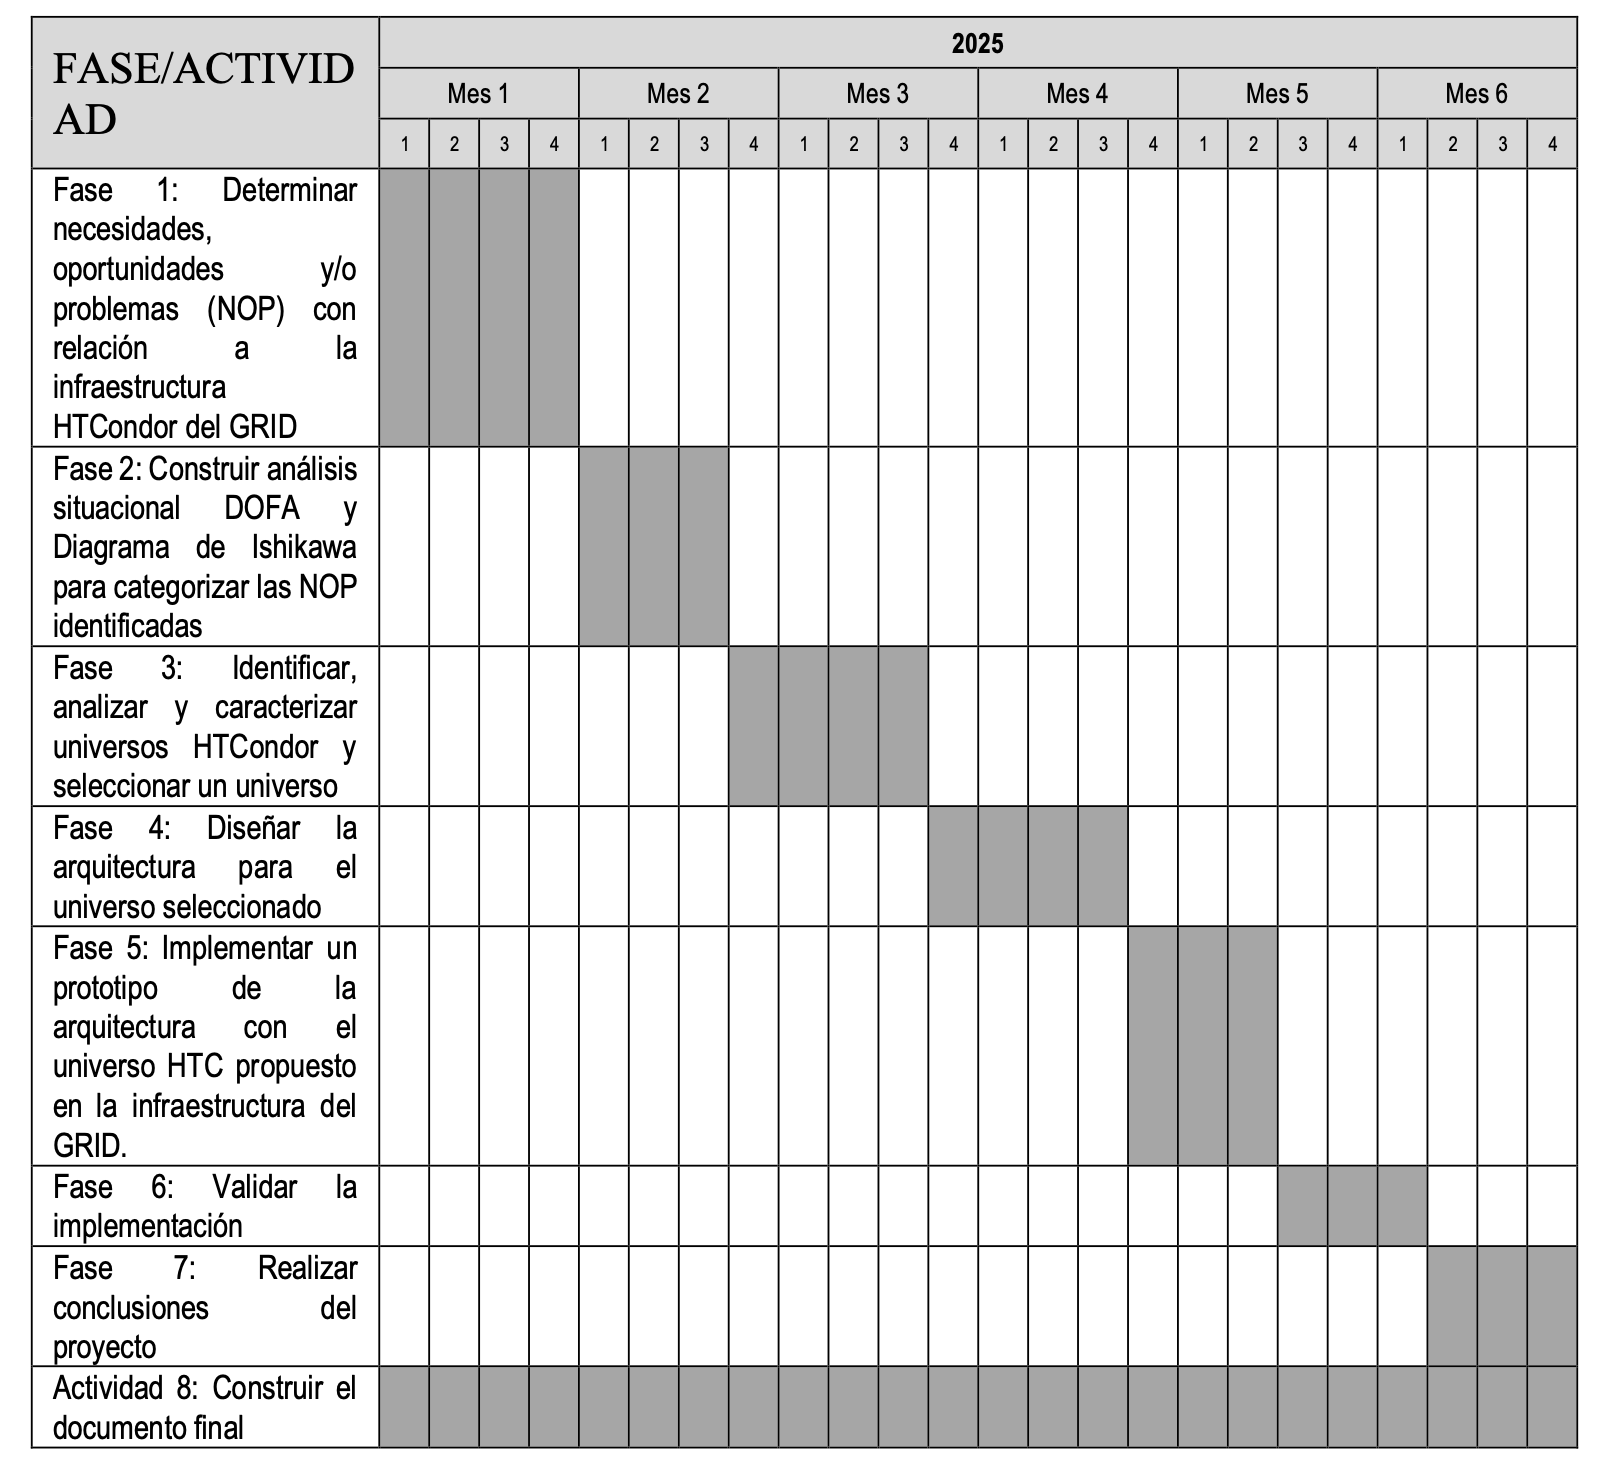
\includegraphics[scale=0.5]{tablas-images/partes/01-generalidades/cronograma.png}
	\caption{Cronograma de actividades del proyecto.}\label{fig:cronograma}
\end{figure}

\ChapterImagePrelim[cap:alcance]{Alcance y delimitación}{./images/fondo.png}\label{cap:alcance}
\mbox{}\\
\noindent
El presente proyecto delimita su alcance a los siguientes aspectos:

\begin{itemize}
	\item Se implementan exclusivamente algoritmos previamente establecidos para su operación en HTCondor, específicamente en el universo seleccionado, garantizando la pertinencia técnica y metodológica.
	\item No se contemplan actividades orientadas a establecer la trazabilidad del caso de negocio entre GRID y los grupos de investigación que recibirán la infraestructura HTCondor, quedando fuera del alcance la integración con otros actores institucionales.
	\item Únicamente son considerados los casos de uso definidos en el contexto del proyecto; cualquier caso externo queda, por tanto, excluido de la presente investigación.
	\item La implementación del universo HTCondor se realiza como un prototipo funcional sobre la infraestructura de los autores, sin comprometer el despliegue en la infraestructura física del grupo de investigación GRID.
\end{itemize}

\ChapterImageStar[cap:objetivos]{Objetivos}{./images/fondo.png}\label{cap:objetivos}
\mbox{}\\

En este capítulo se establece un conjunto de objetivos que orientan el desarrollo del trabajo, articulando el propósito general con metas específicas que permiten su cumplimiento de manera sistemática. Estos objetivos se centran en la definición, análisis y validación de la ampliación de la infraestructura HTCondor del grupo de investigación \GRID, con el fin de responder a las necesidades y oportunidades dicho grupo.

\section{Objetivo general}\label{cap:objetivoGeneral}

Proponer un universo para la ampliación de la infraestructura HTCondor del grupo de investigación \GRID~de la Universidad del Quindío.


\section{Objetivos específicos}\label{cap:objetivosEspecificos}
\begin{itemize}
	\item Determinar necesidades, oportunidades y/o problemas (\NPO) con relación a la infraestructura HTCondor del \GRID.

	\item Identificar, analizar y caracterizar universos HTCondor y seleccionar un universo para la infraestructura del \GRID.

	\item Especificar el diseño arquitectónico requerido para la implementación del universo HTCondor seleccionado.

	\item Implementar un prototipo funcional del universo HTCondor seleccionado según el diseño especificado.

	\item Validar la implementación del universo HTCondor seleccionado según las \NPO~del \GRID.
\end{itemize}
% ...existing code...

\ChapterImageStar[cap:justificacion]{Justificación}{./images/fondo.png}\label{cap:justificacion}
\mbox{}\\

\noindent
En la actualidad, según~\cite{Bianchi2013} la computación distribuida prueba ser una herramienta valiosa para la experimentación tanto científica, experimental como práctica, en cualquiera de las especialidades de ciencias donde se las desee enmarcar. Un claro ejemplo es el análisis de grandes cantidades de datos (\textit{Big Data Analytics}), que según~\cite{Tsai2015} puede utilizar modelos de computación distribuida como uno de sus métodos para gestionar enormes cantidades de información. Además, algunas aplicaciones de software modernas dedicadas a la investigación y el \textit{deep learning} requieren más recursos de los que un solo nodo computacional puede proporcionar; en el caso de esta última, como argumentan~\cite{Thomson2023}, si la carga computacional que requiere el \textit{deep learning} continúa, este terminará por volverse técnica y económicamente prohibitivo.
Además de lo anterior, debe tenerse en cuenta que el grupo de investigación \GRID~realiza investigaciones en temas afines con las redes de computadoras, sistemas distribuidos, seguridad informática, entre otros. La investigación interdisciplinaria y los proyectos con universidades de primer nivel, tanto nacionales como internacionales, son también objetivos alineados con la misión heredada de el \GRID~como lo manifiestan sus integrantes. Así, ampliar la infraestructura HTCondor existente para que soporte un universo adicional y de interés para el \GRID~representa un paso estratégico para alcanzar estos objetivos.
En este contexto, surge una pregunta relevante para el entorno de la Universidad del Quindío: ¿Es justificable ampliar la implementación de la infraestructura HTCondor de el \GRID? Se considera que la respuesta es afirmativa. Factores como el incremento en la capacidad investigativa, el aprovechamiento de recursos computacionales subutilizados, la colaboración con otros grupos de investigación tanto locales como de otras universidades y la mejora en la competitividad de la Universidad del Quindío son razones alineadas con la misión institucional así como de el \GRID.

\ChapterImageStar[cap:marcoConceptual]{Marco Conceptual}{./images/fondo.png}\label{cap:marcoConceptual}
\mbox{}\\

\noindent
Los conceptos a continuación no solo delimitan el ámbito de estudio, sino que también proporcionan las bases terminológicas y estructurales necesarias para la evaluación, comparación e implementación de las tecnologías consideradas.

\noindent
\section{Computación Distribuida}
\noindent
La computación distribuida es un paradigma computacional que involucra dos o más computadoras conectadas en red que trabajan colaborativamente para compartir y ejecutar las mismas tareas computacionales~\citep{Ali2015}. El objetivo fundamental de este enfoque es distribuir las cargas de trabajo a través de múltiples nodos en lugar de depender de una sola máquina. Otra definicíon similar es brindada por ~\cite{Lamport1990}, los cuales argumentan que la computación distribuida es una actividad  de un sistema distribuido espacialmente, \ie, computación extendida a través del espacio; así mismo dan una definición~\cite{Chang1995}, quienes indican que un sistema de computación distribuida es aquel definido como un conjunto de nodos (o procesadores) ubicados en distintos lugares y conectados por una red. Según~\cite{AWS01}, existen cuatro tipos principales de arquitecturas basadas en computación distribuida: (\textbf{1}) la \textbf{arquitectura cliente-servidor}, donde un servidor centralizado proporciona servicios a múltiples clientes que realizan solicitudes; (\textbf{2}) la \textbf{arquitectura de tres niveles}, que separa la lógica en capas de presentación, aplicación y datos para mejorar la escalabilidad y mantenibilidad; (\textbf{3}) la \textbf{arquitectura de N niveles}, que extiende el modelo anterior incorporando múltiples capas especializadas para manejar diferentes aspectos del procesamiento; y (\textbf{4}) la \textbf{arquitectura \textit{peer-to-peer}}, donde todos los nodos actúan simultáneamente como clientes y servidores, compartiendo recursos de manera descentralizada sin depender de un servidor central.

\section{High Throughput Computing (\HTC)}
\noindent
Para~\cite{Morgan2009}, la Computación de Alta Productividad o \textit{High Throughput Computing} (\HTC) constituye una categoría específica de paralelismo computacional que se caracteriza por ejecutar múltiples copias idénticas de una aplicación de manera simultánea. Según los autores, a diferencia del paralelismo de capacidad o ``paralelismo verdadero'', donde los componentes paralelos de una aplicación única se comunican entre sí durante la ejecución, las aplicaciones \HTC~funcionan de manera completamente aislada, requiriendo únicamente una configuración inicial y una comunicación final de resultados. Además, los trabajos \HTC~tienen una naturaleza inherentemente independiente (\ie, no requieren colaboración entre sí), pueden ejecutarse en cualquier orden y pueden ser enviados por distintos usuarios, lo que facilita la gestión distribuida de cargas de trabajo computacionales de gran escala.

\section{Computación de alta productividad \textit{High Peformance Computing} \HPC}

\noindent
Según \cite{SK2023}, \HPC~es aquella computación dedicada al procesamiento paralelo de cálculos complejos a altas velocidades a través de múltiples servidores usando grandes volúmenes de datos. Contrario a la filosofía \HTC, en \HPC~se busca maximizar la cantidad de operaciones de punto flotante (\textit{floating point operations per second} o FLOPS) \citep{HTCondor-what-is-htc}. Mientras que \HPC~se concentra en qué tan rápido se completa un trabajo individual, \HTC~se preocupa por cuántos trabajos se pueden ejecutar a lo largo de períodos extendidos de tiempo, como meses o incluso años \citep{Raman1998}. Esta distinción fundamental establece dos paradigmas complementarios: \HPC~busca el rendimiento \textbf{instantáneo}, mientras que \HTC~busca la productividad \textbf{a largo plazo}.

\section{Matchmaking y ClassAds}
Tanto el Matchmaking como el ClassAd son sistemas diseñados por \cite{Raman1998}. Según estos autores, el Matchmaking constituye un paradigma de gestión de recursos distribuidos diseñado específicamente para entornos de computación de alto rendimiento que se caracteriza por la propiedad distribuida de los recursos y la heterogeneidad del sistema. Los autores argumentan que:

\begin{quote}
	Este enfoque se fundamenta en la premisa de que las entidades que proporcionan o requieren servicios anuncian sus características y requisitos mediante anuncios clasificados (\textit{classified advertisements} o ClassAds), los cuales son procesados por un servicio de emparejamiento designado (\textit{matchmaker}) que identifica coincidencias compatibles e informa a las entidades relevantes, cesando posteriormente su responsabilidad en el proceso. La distinción fundamental de este paradigma radica en la separación clara entre las fases de emparejamiento (\textit{matching}) y reclamación (\textit{claiming}), donde el emparejamiento representa una introducción mutua entre entidades compatibles, mientras que la reclamación establece la relación de trabajo efectiva mediante un protocolo independiente que no involucra al \textit{matchmaker} \citep{Raman1998}.
\end{quote}

\noindent
El sistema ClassAd, por su parte, constituye el modelo de datos semi-estructurado que sustenta el framework de matchmaking, caracterizado por su capacidad de representar servicios arbitrarios y restricciones de asignación sin requerir un esquema específico predefinido~\cite{Raman1998}. Según los autores:
\begin{quote}
	Los ClassAds integran el lenguaje de consulta directamente en el modelo de datos, permitiendo que las restricciones y consultas se expresen como atributos de los propios anuncios, lo que facilita la operación en entornos heterogéneos donde tanto los proveedores de recursos como los clientes pueden imponer restricciones mutuas sobre las entidades con las que están dispuestos a interactuar. Esta arquitectura permite la evaluación de expresiones en un entorno donde cada ClassAd puede acceder a los atributos del otro mediante referencias del tipo ``self.attribute'' y ``other.attribute'', facilitando así la especificación de políticas de uso sofisticadas y dinámicas que se adaptan a las condiciones cambiantes del sistema distribuido \cite{Raman1998}.
\end{quote}


\section{HTCondor}
\noindent
HTCondor es un sistema especializado de gestión de cargas de trabajo diseñado específicamente para trabajos computacionalmente intensivos y enfocado en el paradigma \HTC. Como está expuesto en su página web \citep{HTCondor-what-is-HTCondor}, como otros sistemas de procesamiento por lotes completos, HTCondor proporciona un mecanismo de encolado de trabajos, política de programación, esquema de prioridades, monitoreo de recursos y gestión de recursos. Los usuarios envían sus trabajos seriales o paralelos a HTCondor, que los coloca en una cola, decide cuándo y dónde ejecutar los trabajos basándose en una política específica, monitorea cuidadosamente su progreso e informa al usuario una vez completados \citep{HTCondor-what-is-HTCondor}. La arquitectura innovadora de HTCondor le permite tener éxito en áreas donde los sistemas de programación tradicionales fallan, ya que puede gestionar tanto clústeres de nodos de computación dedicados como aprovechar eficazmente la potencia de \CPU~desperdiciada de estaciones de trabajo de escritorio inactivas. Además, HTCondor incorpora el mecanismo ClassAd que proporciona un marco extremadamente flexible y expresivo para emparejar solicitudes de recursos (trabajos) con ofertas de recursos (máquinas), permitiendo que tanto los trabajos como las máquinas especifiquen requisitos y preferencias de manera sofisticada.

Según la documentación oficial \citep{HTCondor-roles}, en un \textit{pool} de HTCondor, cada máquina puede configurarse para desempeñar uno o más de los siguientes roles fundamentales: el Gestor Central (\textit{master}), el Punto de Acceso (\textit{submit}) y el Punto de Ejecución (\textit{worker}. Estos roles definen las funciones y responsabilidades específicas de cada nodo dentro de la arquitectura distribuida del sistema. Según dicta el manual de \cite{HTCondor-roles}, la descripción de cada rol es como sigue.

El rol más crítico en la arquitectura de HTCondor corresponde al \textbf{Gestor Central} (\textbf{\textit{Central Manager}}). La máquina con este rol tiene la responsabilidad de ejecutar el algoritmo de emparejamiento entre las solicitudes de recursos generadas por los trabajos encolados y los recursos computacionales disponibles en las máquinas de ejecución. El proceso de negociación es orquestado por su demonio principal, \textit{condor\_negotiator}, que implementa las políticas de asignación del sistema. Dada su función coordinadora, el Gestor Central debe desplegarse en una máquina con alta disponibilidad y conectividad de red óptima hacia todos los equipos del \textit{pool}, ya que constituye el punto focal de comunicación para las actualizaciones periódicas de estado provenientes de todos los nodos participantes.

El segundo rol arquitectónico corresponde al \textbf{Punto de Acceso} (\textbf{\textit{Access Point}} o \textit{submit}). Las máquinas configuradas con este rol constituyen la interfaz mediante la cual los usuarios interactúan con la infraestructura HTCondor para someter trabajos al sistema de colas. El demonio \textit{condor\_schedd}, ejecutándose en estos nodos, es responsable de la gestión integral de la cola de trabajos, incluyendo la planificación temporal y la coordinación de las transferencias de archivos de entrada y salida. A diferencia del Gestor Central---cuya singularidad es requisito arquitectónico---pueden coexistir múltiples Puntos de Acceso en un mismo \textit{pool}, facilitando así la escalabilidad horizontal del sistema. Los nodos con este rol deben provisionarse, en lo posible, con abundantes recursos de memoria y capacidad de procesamiento, considerando que por cada nodo ejecutor se instancia un demonio \textit{condor\_shadow} asociado, lo cual puede resultar en demandas significativas de recursos bajo condiciones de alta concurrencia.

El tercer rol fundamental es el de \textbf{Punto de Ejecución} (\textbf{\textit{Execution Point}} o \textit{worker}). Las máquinas configuradas bajo este perfil proveen los recursos computacionales efectivos---ciclos de CPU, memoria RAM, almacenamiento temporal---requeridos para la ejecución material de los trabajos sometidos a HTCondor. El demonio \textit{condor\_startd}, ejecutándose en estos nodos, se encarga de publicar periódicamente la disponibilidad de recursos hacia el Gestor Central mediante mensajes \textit{ClassAd}. Cuando el proceso de negociación resulta en la asignación de un trabajo al nodo, se instancia dinámicamente un proceso \textit{condor\_starter} que asume la responsabilidad de establecer el entorno de ejecución apropiado (\textit{sandbox}), supervisar el ciclo de vida del trabajo y gestionar su terminación. Este rol constituye la clase más poblada en un \textit{pool} típico, pudiendo abarcar desde decenas hasta decenas de miles de máquinas de ejecución en instalaciones de gran escala.

Resulta imperativo destacar que estos roles no son mutuamente exclusivos. Una única máquina física puede ser configurada para desempeñar múltiples roles de forma concurrente, configuración que resulta típica en despliegues de HTCondor de escala reducida o para propósitos de desarrollo y pruebas.\section{Universo}
\noindent
En el contexto del sistema de cómputo distribuido HTCondor, un universo constituye un parámetro de ejecución fundamental que define el entorno operativo y el mecanismo de ejecución específico para una tarea (\textit{job}) enviada al clúster. La documentación oficial del proyecto establece que:

\begin{quote}
	El universo representa el atributo más importante de un trabajo, ya que determina gran parte del comportamiento del sistema HTCondor al gestionar dicho trabajo \citep{HTCondor-what-is-a-job}.
\end{quote}

\noindent
Esta elección configura aspectos críticos como la gestión de procesos, el manejo de archivos, la capacidad de \textit{checkpointing} y migración, e incluso el tipo de aplicación que puede ser ejecutada. Los universos disponibles permiten ejecutar desde binarios estándar y trabajos paralelos MPI hasta máquinas virtuales, contenedores Docker o aplicaciones Java. La diversidad de universos HTCondor incluye opciones como \textit{vanilla} (universo por defecto), \textit{parallel}, \textit{grid}, \textit{container}, \textit{docker}, \textit{java}, \textit{vm}, entre otros, cada uno optimizado para tipos específicos de cargas de trabajo. Por lo tanto, la selección del universo adecuado trasciende la configuración por defecto y constituye un requisito indispensable para garantizar la compatibilidad, eficiencia y éxito en la ejecución de cargas de trabajo heterogéneas en la infraestructura distribuida.

\ChapterImageStar[cap:Marco-Teorico]{Marco Teórico}{./images/fondo.png}\label{cap:marcoTeorico}
\mbox{}\\
\noindent
En el ámbito de la gestión de proyectos y la computación de alto rendimiento, es importante contar con marcos de referencia que ofrezcan una estructura robusta y metodologías para enfrentar los retos actuales. Los conceptos a continuación proporcionan las bases metodológicas, técnicas y estructurales necesarias para el desarrollo e implementación de la ampliación de la infraestructura HTCondor del grupo \GRID.

\section{\PMBOK}
\noindent
En el ámbito de la gestión de proyectos y la computación de alto rendimiento, es importante contar con marcos de referencia que ofrezcan una estructura robusta y metodologías para enfrentar los retos actuales. Este proyecto se fundamenta en el \PMBOK~(\textit{Project Management Body of Knowledge}), que es un estándar reconocido a nivel mundial en la gestión de proyectos y proporciona un conjunto exhaustivo de buenas prácticas aplicables a la mayoría de los proyectos \citep{PMI2019}. Este marco ayuda a la gestión de aspectos importantes como el alcance, tiempo, costo, calidad, recursos humanos, riesgos y comunicación, entre otros.

\section{Normas ISO 9000}
\noindent
Complementando esta perspectiva, las normas ISO 9000 aportan un conjunto de principios y directrices internacionales que permiten a las organizaciones satisfacer las expectativas y necesidades de sus clientes de manera consistente. Estas normas no solo ofrecen un marco sistemático para la mejora continua de los procesos, sino que también propenden por la eficiencia operativa y la calidad de los productos y servicios ofrecidos. En el contexto de este proyecto, su adopción resulta pertinente con el fin de estructurar de forma adecuada las fases de diseño y validación, ayudando así a que el resultado del proyecto sea de calidad y aporte valor al cliente.

\section{Modelo por Capas}
\noindent
Otro pilar conceptual relevante es el modelo por capas, conocido también como arquitectura en capas, que se refiere a una estructura de diseño en la que el sistema se divide en diferentes niveles o capas, cada una con una función específica e independiente de las demás \citep{Spray2023}. Este enfoque resulta especialmente útil en el ámbito de la computación, ya que facilita la escalabilidad, el mantenimiento y la interoperabilidad de los sistemas involucrados. Además, contribuye a reducir la complejidad del diseño y a facilitar la implementación de trabajos futuros inspirados en el presente.

\section{TOGAF (\textit{The Open Group Architecture Framework})}
\noindent
Asimismo, el marco TOGAF, que se ha convertido en uno de los marcos de referencia más utilizados para el desarrollo y gestión de arquitecturas empresariales, proporciona un enfoque estructurado que permite a las organizaciones alinear la estrategia de negocio con los procesos de \TI, facilitando la toma de decisiones y reduciendo el uso de recursos \citep{Mumtaza2025}. Su arquitectura por fases, que abarca la planificación, diseño, implementación y monitoreo, no solo facilita la integración de sistemas y tecnologías, sino que también permite flexibilidad y adaptabilidad en un entorno empresarial en constante evolución.

\section{Estándar ISO/IEC 25010}
\noindent
Además de lo anterior, el estándar ISO/IEC 25010 se incorpora como un estándar internacional que establece un modelo de calidad del software y sistemas, ampliamente utilizado para evaluar la calidad de productos y servicios de \TI. Según lo explica \cite{ISO25010}, este modelo define características como funcionalidad, eficiencia, seguridad, mantenibilidad y usabilidad, proporcionando un marco integral para asegurar que los sistemas cumplan con los requisitos del usuario y del negocio. La implementación de ISO/IEC 25010 en este proyecto responde al deseo de establecer criterios objetivos para validar la utilidad del Universo HTCondor propuesto.


\section{Análisis de Decisiones y Resolución} %!TODO
LOREM IPSUM



\section{Conclusión del Marco de Referencia}
\noindent
En general, el marco de referencia que se propone para este proyecto se basa en teorías y, principalmente, estándares reconocidos internacionalmente, ofreciendo así un soporte metodológico, técnico y estratégico robusto para el diseño y desarrollo de la ampliación de la infraestructura HTCondor del grupo \GRID, permitiéndole a estos avanzar hacia una infraestructura más madura y escalable, alineada con las necesidades actuales de la computación distribuida y de alto rendimiento.





% PARTE 2 DESARROLLO METODOLÓGICO

\ChapterImageStar[cap:revisionLiteratura]{Revisión sistemática de la literatura}{./images/fondo.png}\label{cap:revisionLiteratura}
% !TODO Insertar Taxonomía
\mbox{}\\
\section{Construcción de la bitácora}

En busca de una base teórica sólida para seleccionar un nuevo universo HTCondor y con el objetivo de tomar decisiones informadas, se llevó a cabo una revisión exhaustiva de la literatura existente sobre el tema. Este proceso se desarrolló en varias etapas:


\subsection{Planeación}

Esta etapa tuvo como objetivo definir el propósito general del \SMS (\textit{Systematic Mapping Study}), adoptando la metodología propuesta por \cite{Sepulveda2021}.
A su vez, definió aspectos como objetivos (ver cuadro~\ref{tab:metas}), preguntas de investigación (ver cuadro~\ref{tab:preguntas}) y métricas (ver cuadro~\ref{tab:metricas}). Para ello, se siguió el modelo
Objetivo-Pregunta-Métrica (\textit{goal-question-metric}, GQM).

\subsubsection{Definición de metas para el \SMS}

% Tabla METAS DEL SMS
\begin{table}[H]
	\centering
	\renewcommand{\arraystretch}{1.2} % Espaciado reducido
	\fontsize{9pt}{10pt}\selectfont % Tamaño de fuente 8pt
	\begin{tabular}{|p{1.5cm}|p{12.5cm}|}  % Total: 14cm
		\hline
		\textbf{Meta} & \textbf{Descripción}                                                                                                                                                                                                                                                                                                                                         \\ \hline
		G1            & Clasificar trabajos relacionados con los universos de HTCondor según su aplicación e impacto en los dominios de computación distribuida y paralela, HTC, desarrollo de Software, virtualización y microservicios, redes de computadoras, infraestructura computacional, inteligencia artificial, análisis de datos y pensamiento computacional, entre otros. \\ \hline
		G2            & Identificar y categorizar trabajos vinculados con los universos de HTCondor como herramienta para fortalecer funciones esenciales universitarias como: investigación, docencia, extensión e industria.                                                                                                                                                       \\ \hline
	\end{tabular}
	\caption{Definición de metas del SMS}
	\label{tab:metas}
\end{table}


\subsubsection{Definición de preguntas de investigación}\label{subsubsec:RQ-def}
%TABLA GOAL VS Preguntas
\begin{table}[H]
	\centering
	\renewcommand{\arraystretch}{1.2} % Espaciado reducido
	\fontsize{9pt}{10pt}\selectfont % Tamaño de fuente 8pt
	\begin{tabular}{|p{0.7cm}|p{1.3cm}|p{5.5cm}|p{6cm}|} % Total: 14cm
		\hline
		\textbf{Meta}                                                                                                                                                                                                                                                                                                                                    & \textbf{Pregunta} & \textbf{Descripción} & \textbf{Motivación}        \\ \hline

		G1                                                                                                                                                                                                                                                                                                                                               & Q1                &
		\textit{¿Qué trabajos relacionados con los universos de HTCondor tienen impacto en los dominios de computación distribuida y paralela, HTC, desarrollo de Software, virtualización y microservicios, redes de computadoras, infraestructura computacional, inteligencia artificial, análisis de datos y pensamiento computacional, entre otros?} &
		Sobre los universos de HTCondor que tienen impacto en los dominios de computación distribuida y paralela, \HTC, desarrollo de Software, virtualización y microservicios, redes de computadoras, infraestructura computacional, inteligencia artificial, análisis de datos, pensamiento computacional: 1 - Reconocer cómo están estructurados. 2 - Identificar sus aplicaciones. 3 - Determinar su motivación contextual. \\ \hline

		G2                                                                                                                                                                                                                                                                                                                                               & Q2                &
		\textit{¿Qué trabajos vinculados con los universos de HTCondor potencian las funciones esenciales universitarias como investigación, docencia, extensión e industria?}                                                                                                                                                                           &
		Sobre los universos de HTCondor que potencian las funciones sustantivas universitarias como investigación, docencia, extensión e industria: 1 - Reconocer cómo están estructurados. 2 - Identificar sus aplicaciones. 3 - Determinar su motivación contextual.                                                                                                                                                           \\ \hline
	\end{tabular}
	\caption{Definición de preguntas de investigación del SMS}
	\label{tab:preguntas}
\end{table}

\subsubsection{Definición de métricas}
%Tabla METRICAS
\begin{table}[H]
	\centering
	\renewcommand{\arraystretch}{1.2} % Menor espaciado entre filas
	\fontsize{9pt}{10pt}\selectfont % Tamaño de fuente 8pt
	\begin{tabular}{|c|p{13cm}|} % Total: 14cm
		\hline
		\textbf{Métrica} & \textbf{Descripción}                                                                                                                                                                                                                                                                                                                                                                                                                                                                                           \\ \hline
		M1               & Cantidad de trabajos relacionados con los Universos de HTCondor vinculados con los dominios de: Computación distribuida y paralela, HTC, Desarrollo de software, Tecnologías de virtualización y microservicios, Redes de computadores, Infraestructura computacional, Inteligencia artificial, Análisis de datos, Pensamiento computacional, entre otros. Y que además sean usados como herramienta para fortalecer funciones esenciales universitarias como: Investigación, Docencia, Extensión e Industria. \\ \hline
		M2               & Popularidad de cada Universo en los trabajos seleccionados.                                                                                                                                                                                                                                                                                                                                                                                                                                                    \\ \hline
		M3               & Porcentaje de trabajos seleccionados en la fase final respecto de la cantidad de trabajos iniciales.                                                                                                                                                                                                                                                                                                                                                                                                           \\ \hline
		M4               & Porcentaje de trabajos aportados por cada base de datos en el mapeo que se está desarrollando.                                                                                                                                                                                                                                                                                                                                                                                                                 \\ \hline
	\end{tabular}
	\caption{Definición de métricas del SMS}
	\label{tab:metricas}
\end{table}


\newpage \section{Búsqueda de estudios}


Esta etapa comprendió las siguientes secciones:
\begin{enumerate}
	\item Estrategia de búsqueda, ya sea independiente o combinada;
	\item Identificación general de estudios;
	\item Revisión de estudios; y finalmente,
	\item Selección de estudios para incluir en el SMS.\@
\end{enumerate}

\subsection{Estrategia de búsqueda}

Este trabajo combinó estrategias de búsqueda en bases de datos con la técnica de búsqueda en bola de nieve, lo que permitió ampliar y enriquecer la recopilación de estudios relevantes para el mapeo sistemático. Esta aproximación facilitó la identificación de investigaciones clave que podrían no haber sido detectadas mediante una búsqueda tradicional.

\subsection{Búsqueda en bases de datos}\label{subsec:busquedaBasesDatos}
Se seleccionaron las siguientes bases de datos para llevar a cabo el mapeo sistemático de estudios: ACM, IEEE Xplore, Springer, Taylor \& Francis y Science Direct. Estas fuentes fueron elegidas por su disponibilidad, relevancia y cobertura en el área de investigación, asegurando así la obtención de información actualizada y de calidad para el desarrollo del estudio.


\newpage
\subsubsection{Identificación de estudios mediante búsqueda en bases de datos}\label{subsubsec:identificacionEstudios}
En esta etapa del proceso fue necesario establecer un marco que ayudase a establecer las palabras clave más apropiadas para el mapeo sistemático de estudios para cada una de las bases de datos seleccionadas. Para ello se hizo uso del modelo PICOC (\textit{Population}, \textit{Intervention}, \textit{Comparator}, \textit{Outcome}, and \textit{Context}) como guía metodológica, sirviendo como herramienta de apoyo para este procedimiento. El resultado de este proceso puede verse en la tabla~\ref{table:modelo-picoc}

% TABLA modelo PICOC: Población - Intervención - Comparación  - Salida - Contexto
\begin{table}[H]
	\centering
	\renewcommand{\arraystretch}{1.5} % Espaciado reducido
	\fontsize{9pt}{10pt}\selectfont % Tamaño de fuente 8pt
	\begin{tabular}{|c|p{12cm}|} % Total: 14cm
		\hline
		\textbf{Componente} & \textbf{Descripción}                                                                                                                                                                                                                                                                                                                                                                                                                                                                             \\ \hline

		Población           & Trabajos relacionados con los universos de HTCondor según su aplicación e impacto en los dominios de computación distribuida y paralela, HTC, desarrollo de Software, virtualización y microservicios, redes de computadoras, infraestructura computacional, inteligencia artificial, análisis de datos, pensamiento computacional, entre otros. Que potencian las funciones sustantivas universitarias de investigación, docencia y extensión.                                                  \\ \hline

		Intervención        & Identificación y clasificación de un conjunto de trabajos relacionados con los universos de HTCondor según su aplicación e impacto en los dominios de computación distribuida y paralela, HTC, desarrollo de Software, virtualización y microservicios, redes de computadoras, infraestructura computacional, inteligencia artificial, análisis de datos, pensamiento computacional, entre otros. Que potencian las funciones sustantivas universitarias de investigación, docencia y extensión. \\ \hline

		Comparación         &
		\textbf{1.} Casos de proyecto documentados.
		\textbf{2.} Cumplimiento de criterios de inclusión y exclusión.
		\textbf{3.} Aparición en bases de datos seleccionadas.                                                                                                                                                                                                                                                                                                                                                                                                                                                                 \\ \hline
		Salida              & Taxonomía que organiza los trabajos relacionados con los universos de HTCondor según su aplicación e impacto en los dominios de computación distribuida y paralela, HTC, desarrollo de Software, virtualización y microservicios, redes de computadoras, infraestructura computacional, inteligencia artificial, análisis de datos, pensamiento computacional, entre otros. Que potencian las funciones sustantivas universitarias de investigación, docencia y extensión.                       \\ \hline
		Contexto            & Universos HTCondor en dominios de computación distribuida y paralela, HTC, desarrollo de Software, virtualización y microservicios, redes de computadoras, infraestructura computacional, inteligencia artificial, análisis de datos, pensamiento computacional, entre otros. Que potencian las funciones sustantivas universitarias de investigación, docencia y extensión.                                                                                                                     \\ \hline
	\end{tabular}
	\caption{Modelo PICOC}
	\label{table:modelo-picoc}
\end{table}



%# TABLA Palabras clave indentificadas usando el modelo PICOC.
\begin{table}[H]
	\centering
	\renewcommand{\arraystretch}{1.4}
	\fontsize{8}{8}\selectfont
	\begin{tabular}{|p{3cm}|p{10.0cm}|}
		\hline
		\textbf{Categoría \hbox{PICOC}} & \textbf{Palabras clave} \\
		\hline
		Población                       &
		- Trabajos relacionados \newline
		- Universos \newline
		- HTCondor \newline
		- Computación distribuida y paralela \newline
		- HTC \newline
		- Desarrollo de Software \newline
		- Virtualización y microservicios \newline
		- Redes de computadoras \newline
		- Infraestructura computacional \newline
		- Inteligencia artificial \newline
		- Análisis de datos \newline
		- Pensamiento computacional \newline
		- Investigación \newline
		- Docencia \newline
		- Extensión                                               \\
		\hline
		Intervención                    &
		- Identificación \newline
		- Clasificación \newline
		- Universos \newline
		- HTCondor \newline
		- Computación distribuida y paralela \newline
		- HTC \newline
		- Desarrollo de Software \newline
		- Virtualización y microservicios \newline
		- Redes de computadoras \newline
		- Infraestructura computacional \newline
		- Inteligencia artificial \newline
		- Análisis de datos \newline
		- Pensamiento computacional \newline
		- Investigación \newline
		- Docencia \newline
		- Extensión                                               \\
		\hline
		Criterios de aceptación         &
		- Casos de estudio culminados                             \\
		\hline
		Salidas                         &
		- Taxonomía \newline
		- Universos \newline
		- HTCondor \newline
		- Computación distribuida y paralela \newline
		- HTC \newline
		- Desarrollo de Software \newline
		- Virtualización y microservicios \newline
		- Redes de computadoras \newline
		- Infraestructura computacional \newline
		- Inteligencia artificial \newline
		- Análisis de datos \newline
		- Pensamiento computacional \newline
		- Investigación \newline
		- Docencia \newline
		- Extensión                                               \\
		\hline
		Contexto                        &
		- Universos \newline
		- HTCondor \newline
		- Computación distribuida y paralela \newline
		- HTC \newline
		- Desarrollo de Software \newline
		- Virtualización y microservicios \newline
		- Redes de computadoras \newline
		- Infraestructura computacional \newline
		- Inteligencia artificial \newline
		- Análisis de datos \newline
		- Pensamiento computacional \newline
		- Investigación \newline
		- Docencia \newline
		- Extensión                                               \\
		\hline
	\end{tabular}
	\caption{Palabras clave identificadas usando el modelo PICOC}
	\label{table:keywords-picoc}
\end{table}

Las palabras clave identificadas en el cuadro~\ref{table:keywords-picoc} se complementaron con sinónimos y términos relacionados, los cuales se presentan en el cuadro~\ref{tab:keywords}. Estas keywords se utilizaron para construir las cadenas de búsqueda en cada base de datos.


%# TABLA Keywoords para las cadenas de búsqueda,
\begin{table}[H]
	\centering
	\scriptsize
	\setlength{\tabcolsep}{4pt}
	\fontsize{9pt}{10pt}\selectfont % Tamaño de fuente 8pt
	\begin{tabular}{|c|p{12.5cm}|} % Total: 14cm
		\hline
		\textbf{Palabras clave} & \textbf{Sinónimos}                                                             \\
		\hline
		HTCondor                & High Throughput Condor, Distributed Computing Framework, Condor                \\
		\hline
		HTC                     & HPC, High Throughput Computing, High Performance Computing                     \\
		\hline
		Universe                & Execution Environment, Runtime Environment, Cluster                            \\
		\hline
		Project                 & Work, Implementation, Implement, Deployment, Development, Program, Plan, Study \\
		\hline
		Research                & Teaching, Extension, Outreach, Industry                                        \\
		\hline
	\end{tabular}
	\caption{Palabras clave para la búsqueda en base de datos}
	\label{tab:keywords}
\end{table}



\noindent
Con el objetivo de filtrar los resultados y enfocarse en estudios relevantes, se definieron criterios de inclusión y exclusión, los cuales se presentan en el cuadro~\ref{table:criterios-inclusion-exclusion}. Estos criterios ayudaron a seleccionar artículos que se alinean con los objetivos del \SMS y a descartar aquellos que no aportan valor al análisis.

% TABLA Criterios de inclusión y exclusión
\begin{table}[H]
	\centering
	\caption{Criterios de inclusión y exclusión}
	\fontsize{9pt}{10pt}\selectfont % Tamaño de fuente 8pt
	\begin{tabular}{|p{3cm}|p{5cm}|p{6cm}|}
		\hline
		\textbf{Categoría}  & \textbf{Inclusión}         & \textbf{Exclusión}                                                                                                          \\
		\hline
		Tipo de publicación & Artículos de investigación & Tesis, capítulos de libros, libros, revistas, conferencias, y todo lo demás que no esté en el tipo de publicación inclusiva \\
		\hline
		Período             & Desde 2020 hasta 2024      & -                                                                                                                           \\
		\hline
		Idioma              & Inglés                     & -                                                                                                                           \\
		\hline
	\end{tabular}
	\label{table:criterios-inclusion-exclusion}
\end{table}



%##################
%##################
%##################
%##################
%##################




\subsubsection{Búsqueda en bases de datos}\label{par:busquedaBasesDatos}
\noindent
Las cadenas de búsqueda específicas para cada base de datos se encuentran en la sección~\ref{sec:cadenas-busqueda} del apéndice.

\subsubsection{Métricas de la búsqueda sin criterios de inclusión/exclusión}\label{subsubsec:resumenBusqueda}
\noindent
La Tabla~\ref{table:bases-sin-exclusion} presenta el número de publicaciones identificadas en las principales bases de datos consultadas durante la revisión inicial de literatura, antes de aplicar los criterios de inclusión y exclusión. En total se recuperaron 847 registros, distribuidos de la siguiente manera: ACM (518), IEEE (0), Springer (209), Science Direct (120) y Taylor \& Francis (0). Estos resultados se evidencian en el apéndice~\ref{sec:busqueda-sin-criterios}.

% TABLA Resultados de busqueda sin exclusión
\begin{table}[H]
	\centering
	\caption{Resultados de las cadenas de búsqueda}
	\label{table:bases-sin-exclusion}
	\fontsize{8pt}{10pt}\selectfont % Tamaño de fuente 8pt
	\begin{tabular}{|p{3.5cm}|>{\centering\arraybackslash}p{1.0cm}|>{\centering\arraybackslash}p{1.0cm}|>{\centering\arraybackslash}p{2.0cm}|>{\centering\arraybackslash}p{1.3cm}|>{\centering\arraybackslash}p{2.3cm}|>{\centering\arraybackslash}p{1.0cm}|}
		\hline
		\textbf{Criterios}                               & \textbf{ACM} & \textbf{IEEE} & \textbf{ScienceDirect} & \textbf{Springer} & \textbf{Taylor\&Francis} & \textbf{Total} \\
		\hline
		Cadena de búsqueda con palabras clave únicamente & 518          & 0             & 120                    & 209               & 0                        & 847            \\
		\hline
		Contribución porcentual                          & 61.16\%      & 0\%           & 14.17\%                & 24.68\%           & 0\%                      & 100\%          \\
		\hline
	\end{tabular}
\end{table}





\subsubsection{Métricas de la búsqueda con criterios de inclusión/exclusión}\label{subsec:resumenBusquedaCriterios}
\noindent
Esta búsqueda se realizó considerando los criterios de exclusión e inclusión definidos previamente. Las cadenas de búsqueda son exactamente iguales que antes, este punto se diferencia por la aplicación de filtros. Para ver las capturas de pantalla veáse el apéndice~\ref{sec:busqueda-con-criterios}.
La Tabla~\ref{table:bases-con-exclusion} muestra los resultados obtenidos tras aplicar los criterios de inclusión y exclusión previamente definidos. A diferencia de la búsqueda inicial, en esta fase se utilizaron filtros específicos que redujeron significativamente la cantidad de publicaciones relevantes. En total se identificaron 976 documentos, distribuidos en las bases de datos de la siguiente manera: ACM (48), IEEE (134), Springer (592), Science Direct (46) y Taylor \& Francis (156).

% TABLA Bases de datos con inclusión
\begin{table}[H]
	\centering
	\caption{Resultados de las cadenas de búsqueda con criterios de exclusión}
	\label{table:bases-con-exclusion}
	\fontsize{8pt}{10pt}\selectfont % Tamaño de fuente 8pt
	\begin{tabular}{|p{3.5cm}|>{\centering\arraybackslash}p{1.0cm}|>{\centering\arraybackslash}p{1.0cm}|>{\centering\arraybackslash}p{2.0cm}|>{\centering\arraybackslash}p{1.3cm}|>{\centering\arraybackslash}p{2.3cm}|>{\centering\arraybackslash}p{1.0cm}|}
		\hline
		\textbf{Criterios}                               & \textbf{ACM} & \textbf{IEEE} & \textbf{ScienceDirect} & \textbf{Springer} & \textbf{Taylor \& Francis} & \textbf{Total} \\
		\hline
		Cadena de búsqueda con palabras clave únicamente & 315          & 0             & 101                    & 63                & 0                          & 479            \\
		\hline
		Contribución porcentual                          & 65.76\%      & 0\%           & 21.09\%                & 13.15\%           & 0\%                        & 100\%          \\
		\hline
	\end{tabular}
\end{table}

El fruto del proceso logrado en la búsqueda de bases de datos puede verse en la figura \ref{fig:resumen-busqueda-bases-de-datos}. Como se puede observar, luego de aplicación de los criterios de exclusión, se perdieron 368 estudios, un perdida porcentual del 43.44\% respecto los resultados de la búsqueda inicial.

% FIGURA de resultados de ambos procesos de busqueda con y sin criterios.
\begin{figure}[H]
	\centering
	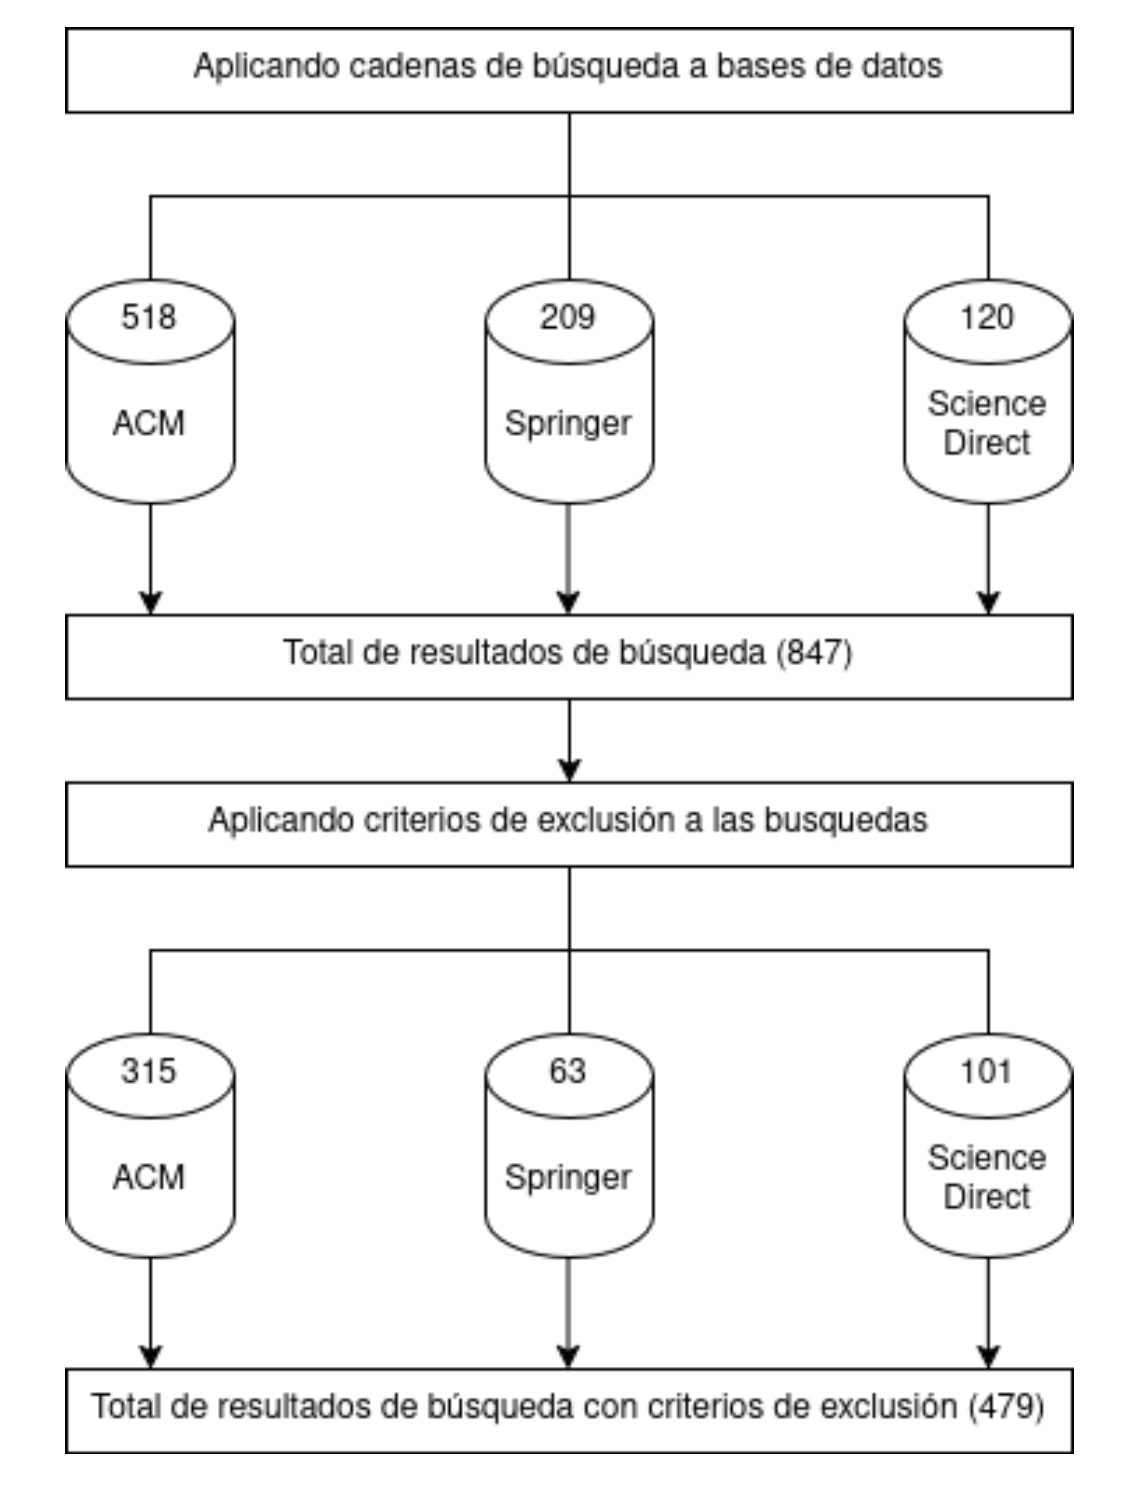
\includegraphics[scale=0.6] {tablas-images/sms/resumen_busqueda_bases.png}
	\caption{Diagrama resumen del proceso de búsqueda en bases de datos}\label{fig:resumen-busqueda-bases-de-datos}
\end{figure}




\section{Eliminación de duplicados}\label{sec:eliminacionDuplicados}
\noindent
La eliminación de estudios duplicados se efectuó mediante la herramienta de gestión bibliográfica Mendeley. Tras la recopilación inicial, todos los artículos fueron importados a dicha plataforma, la cual identificó y eliminó automáticamente las publicaciones redundantes. Este proceso resultó en la exclusión de \textbf{tres} artículos duplicados, reduciendo el total de estudio a 476. La figura \ref{fig:eliminacion-duplicados} presenta una visualización gráfica de estos resultados.


% FIGURA Eliminación de duplicados
\begin{figure}[H]
	\centering
	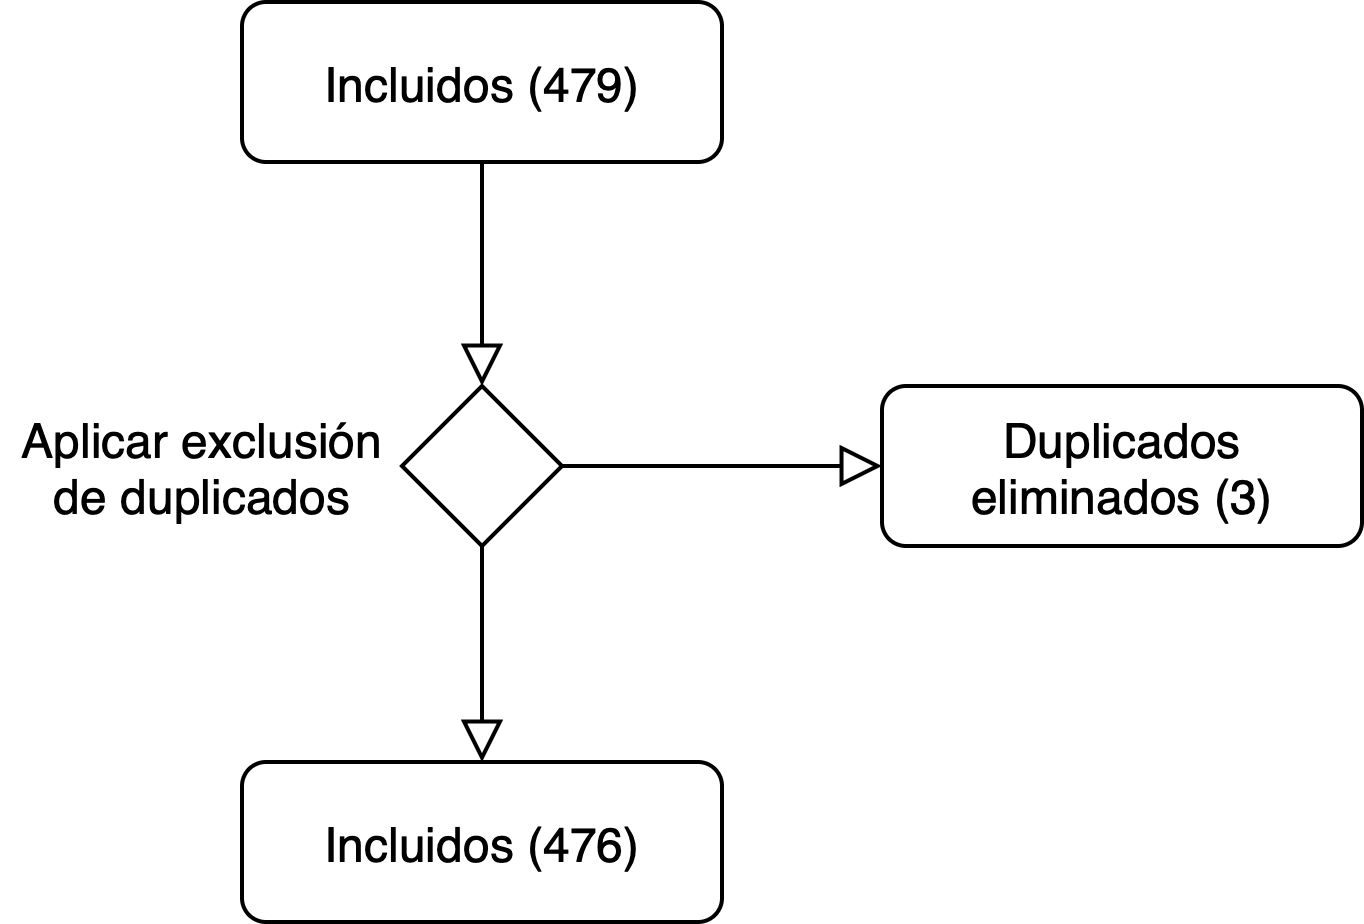
\includegraphics[scale=0.25] {tablas-images/sms/eliminacion-duplicados.png}
	\caption{Diagrama del proceso de eliminación de resultados}\label{fig:eliminacion-duplicados}
\end{figure}


\section{Priorización de estudios}\label{sec:priorizacionEstudios}
\noindent


Luego de la selección inicial de los artículos, se procedió a examinar los campos  \textit{title}, \textit{abstract} y \textit{keywords} de cada uno. Como resultado de esta revisión se generaron métricas de calidad para cada artículo, con el fin de priorizar aquellos más relevantes para la investigación. Las métricas utilizadas fueron las siguientes:

\begin{itemize}
	\item \textbf{SCI} \textit{(Science Citation Index)}
	\item \textbf{CVI} \textit{(Core Value Index)}
	\item \textbf{IRRQ} \textit{(Index Relation Research Question)}
\end{itemize}
\noindent

Este proceso inició con un total de 476 artículos, los cuales fueron evaluados según su alineamiento con los objetivos de la investigación. La evaluación temática permitió identificar un total de 99 artículos con una relación directa con el enfoque planteado.

\section{Estrategia de búsqueda usando bola de nieve}\label{sec:bolaDeNieve}
\noindent

En esta etapa, se seleccionó el primer cuartil según el índice \SCI, obteniendo un total de 24 artículos que constituyeron la línea base para el proceso de búsqueda por bola de nieve. A partir de esta base, se aplicó la estrategia de bola de nieve en ambas direcciones: hacia adelante (revisando referencias citadas por los artículos base) y hacia atrás (identificando artículos que citan a los de la base). En la primera iteración se obtuvieron tres artículos mediante la técnica hacia atrás y cuatro mediante la técnica hacia adelante. La segunda iteración produjo tres artículos adicionales con bola de nieve hacia atrás y cinco con bola de nieve hacia adelante. En total, el proceso de bola de nieve generó 15 artículos adicionales. Sumando estos resultados a los 99 artículos previamente filtrados por \SCI, se obtuvo un corpus final de 114 artículos para el análisis.

El resumen de este proceso puede verse en la figura \ref{fig:resumen-snowball}

\begin{figure}[H]
	\begin{center}
		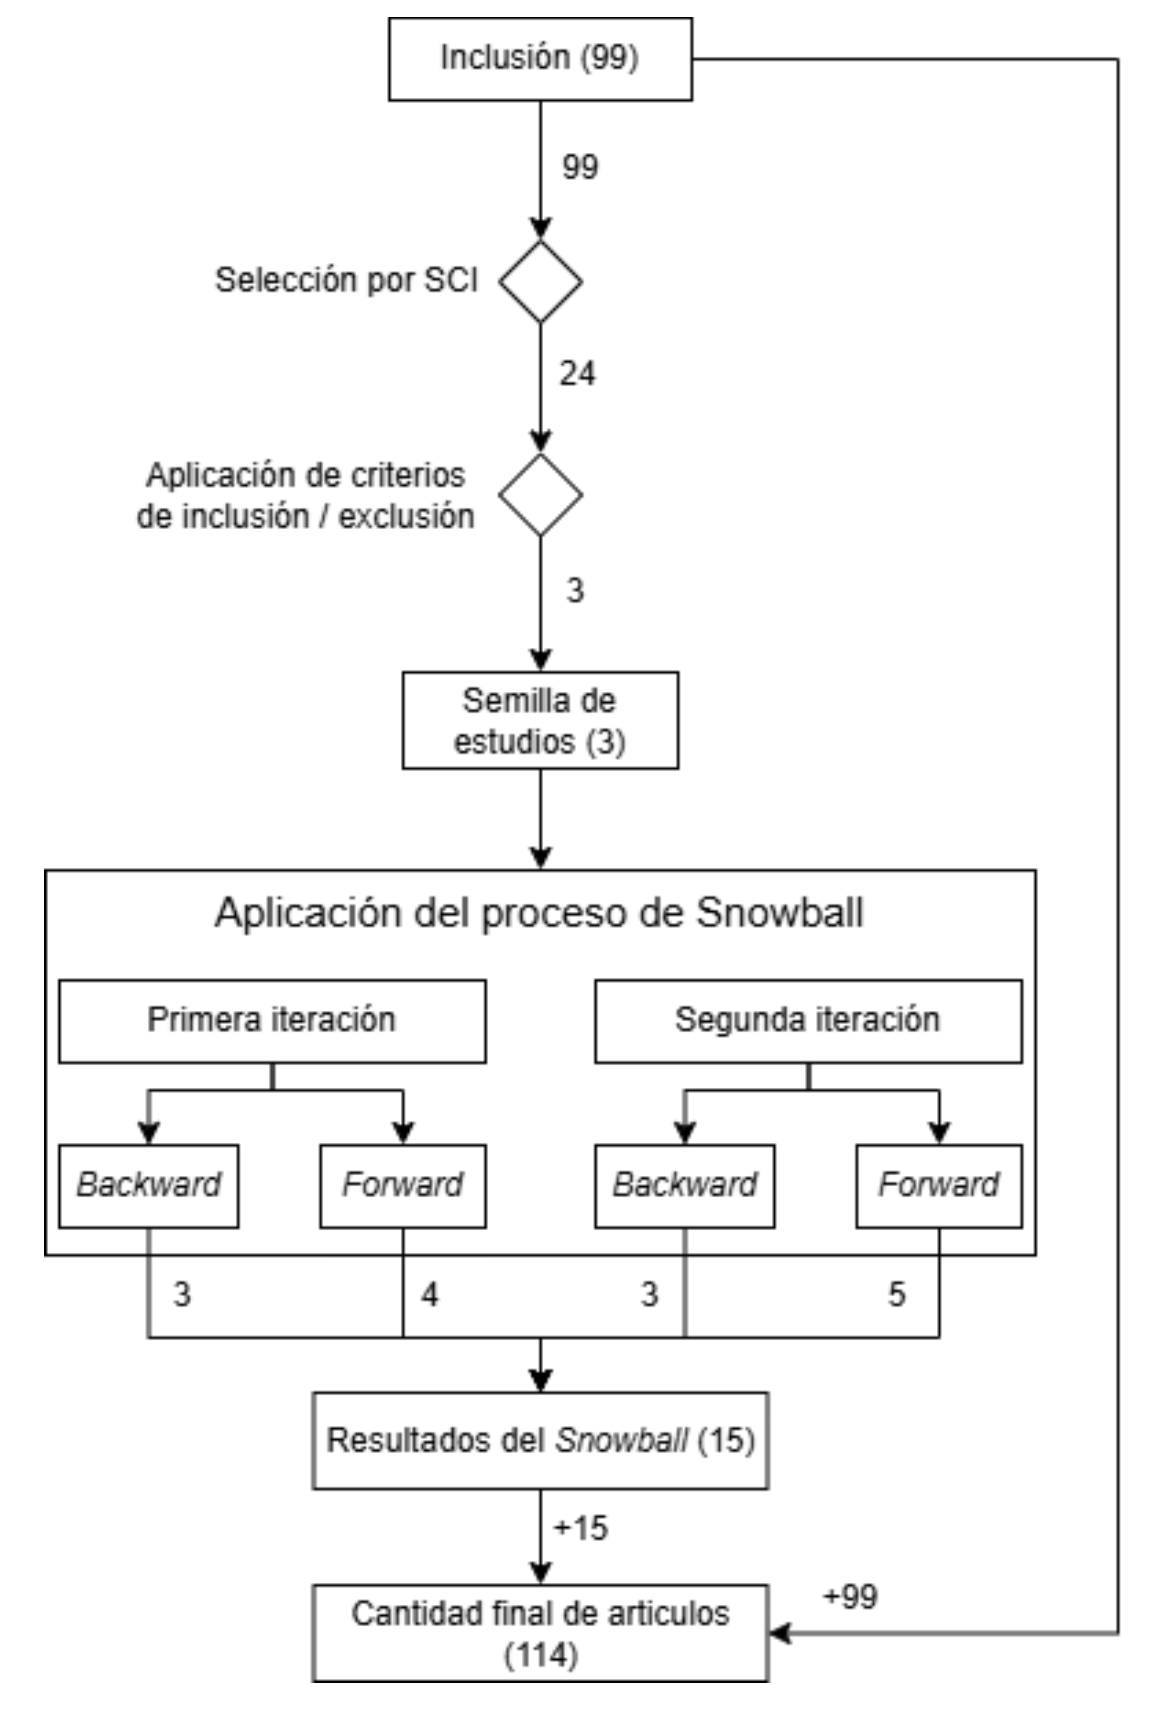
\includegraphics[width=0.6\textwidth]{tablas-images/sms/resumen-snowball.png}
	\end{center}
	\caption{}\label{fig:resumen-snowball}
\end{figure}


\section{Identificación de estudios}

\section{Cuadro de estudios}

Los estudios resultantes del proceso de \SMS se presentan en la tabla \ref{table:selected_primary_studies}.



% -------- Tabla : Estudios Primarios Seleccionados (SPSs) ------------
\begin{table}[H]
	\centering
	\caption{Los 114 estudios primarios seleccionados (SPSs)}
	\label{table:selected_primary_studies}
	\fontsize{8pt}{10pt}\selectfont % Tamaño de fuente 8pt
	\renewcommand{\arraystretch}{1.2}
	\begin{tabular*}{\textwidth}{l @{\extracolsep{\fill}} r l @{\extracolsep{\fill}} r l @{\extracolsep{\fill}} r l @{\extracolsep{\fill}} r l @{\extracolsep{\fill}} r}
		\toprule
		\textbf{ID} & \textbf{Ref}                        & \textbf{ID} & \textbf{Ref}                        & \textbf{ID} & \textbf{Ref}                      & \textbf{ID} & \textbf{Ref}                        & \textbf{ID} & \textbf{Ref}                       \\
		\midrule
		SPS001      & \spsone                             & SPS002      & \spstwo                             & SPS003      & \spsthree                         & SPS004      & \spsfour                            & SPS005      & \spsfive                           \\
		SPS006      & \spssix                             & SPS007      & \spsseven                           & SPS008      & \spseight                         & SPS009      & \spsnine                            & SPS010      & \spsten                            \\
		SPS011      & \spseleven                          & SPS012      & \spstwelve                          & SPS013      & \spsthirteen                      & SPS014      & \spsfourteen                        & SPS015      & \spsfifteen                        \\
		SPS016      & \spssixteen                         & SPS017      & \spsseventeen                       & SPS018      & \spseighteen                      & SPS019      & \spsnineteen                        & SPS020      & \spstwenty                         \\
		SPS021      & \spstwentyone                       & SPS022      & \spstwentytwo                       & SPS023      & \spstwentythree                   & SPS024      & \spstwentyfour                      & SPS025      & \spstwentyfive                     \\
		SPS026      & \spstwentysix                       & SPS027      & \spstwentyseven                     & SPS028      & \spstwentyeight                   & SPS029      & \spstwentynine                      & SPS030      & \spsthirty                         \\
		SPS031      & \spsthirtyone                       & SPS032      & \spsthirtytwo                       & SPS033      & \spsthirtythree                   & SPS034      & \spsthirtyfour                      & SPS035      & \spsthirtyfive                     \\
		SPS036      & \spsthirtysix                       & SPS037      & \spsthirtyseven                     & SPS038      & \spsthirtyeight                   & SPS039      & \spsthirtynine                      & SPS040      & \spsforty                          \\
		SPS041      & \spsfortyone                        & SPS042      & \spsfortytwo                        & SPS043      & \spsfortythree                    & SPS044      & \spsfortyfour                       & SPS045      & \spsfortyfive                      \\
		SPS046      & \spsfortysix                        & SPS047      & \spsfortyseven                      & SPS048      & \spsfortyeight                    & SPS049      & \spsfortynine                       & SPS050      & \spsfifty                          \\
		SPS051      & \spsfiftyone                        & SPS052      & \spsfiftytwo                        & SPS053      & \spsfiftythree                    & SPS054      & \spsfiftyfour                       & SPS055      & \spsfiftyfive                      \\
		SPS056      & \spsfiftysix                        & SPS057      & \spsfiftyseven                      & SPS058      & \spsfiftyeight                    & SPS059      & \spsfiftynine                       & SPS060      & \spssixty                          \\
		SPS061      & \spssixtyone                        & SPS062      & \spssixtytwo                        & SPS063      & \spssixtythree                    & SPS064      & \spssixtyfour                       & SPS065      & \spssixtyfive                      \\
		SPS066      & \spssixtysix                        & SPS067      & \spssixtyseven                      & SPS068      & \spsixtyeight                     & SPS069      & \spssixtynine                       & SPS070      & \spsseventy                        \\
		SPS071      & \spsseventyone                      & SPS072      & \spsseventytwo                      & SPS073      & \spsseventythree                  & SPS074      & \spsseventyfour                     & SPS075      & \spsseventyfive                    \\
		SPS076      & \spsseventysix                      & SPS077      & \spsseventyseven                    & SPS078      & \spsseventyeight                  & SPS079      & \spsseventynine                     & SPS080      & \spseighty                         \\
		SPS081      & \spseightyone                       & SPS082      & \spseightytwo                       & SPS083      & \spseightythree                   & SPS084      & \spseightyfour                      & SPS085      & \spseightyfive                     \\
		SPS086      & \spseightysix                       & SPS087      & \spseightyseven                     & SPS088      & \spseightyeight                   & SPS089      & \spseightynine                      & SPS090      & \spsninety                         \\
		SPS091      & \spsninetyone                       & SPS092      & \spsninetytwo                       & SPS093      & \spsninetythree                   & SPS094      & \spsninetyfour                      & SPS095      & \spsninetyfive                     \\
		SPS096      & \spsninetysix                       & SPS097      & \spsninetyseven                     & SPS098      & \spsnineyeight                    & SPS099      & \spsninetynine                      & SPS100      & \spsonehundred                     \\
		SPS101      & \spsonehundredone                   & SPS102      & \spsonehundredtwo                   & SPS103      & \spsonehundredthree               & SPS104      & \spsonehundredfour                  & SPS105      & \spsonehundredfive                 \\
		SPS106      & \spsonehundredsix                   & SPS107      & \spsonehundredseven                 & SPS108      & \spsonehundredeight               & SPS109      & \spsonehundrednine                  & SPS110      & \spsonehundredten                  \\
		SPS111      & \spsonehundredeleven                & SPS112      & \spsonehundredtwelve                & SPS113      & \spsonehundredthirteen            & SPS114      & \spsonehundredfourteen              &             &                                    \\
		\bottomrule
	\end{tabular*}
	\vspace{5pt}
\end{table}

%  --------------------------------------------------------------


\subsection{Artículos por año y métricas}
\noindent
A continuación se presentan las gráficas de los resultados de la búsqueda. En la figura \ref{fig:plot-anios-vs-indices-calidad} se muestra la relación entre la cantidad de estudios por año y las métricas definidas en las sección \ref{sec:priorizacionEstudios}

\begin{figure}[H]
	\begin{center}
		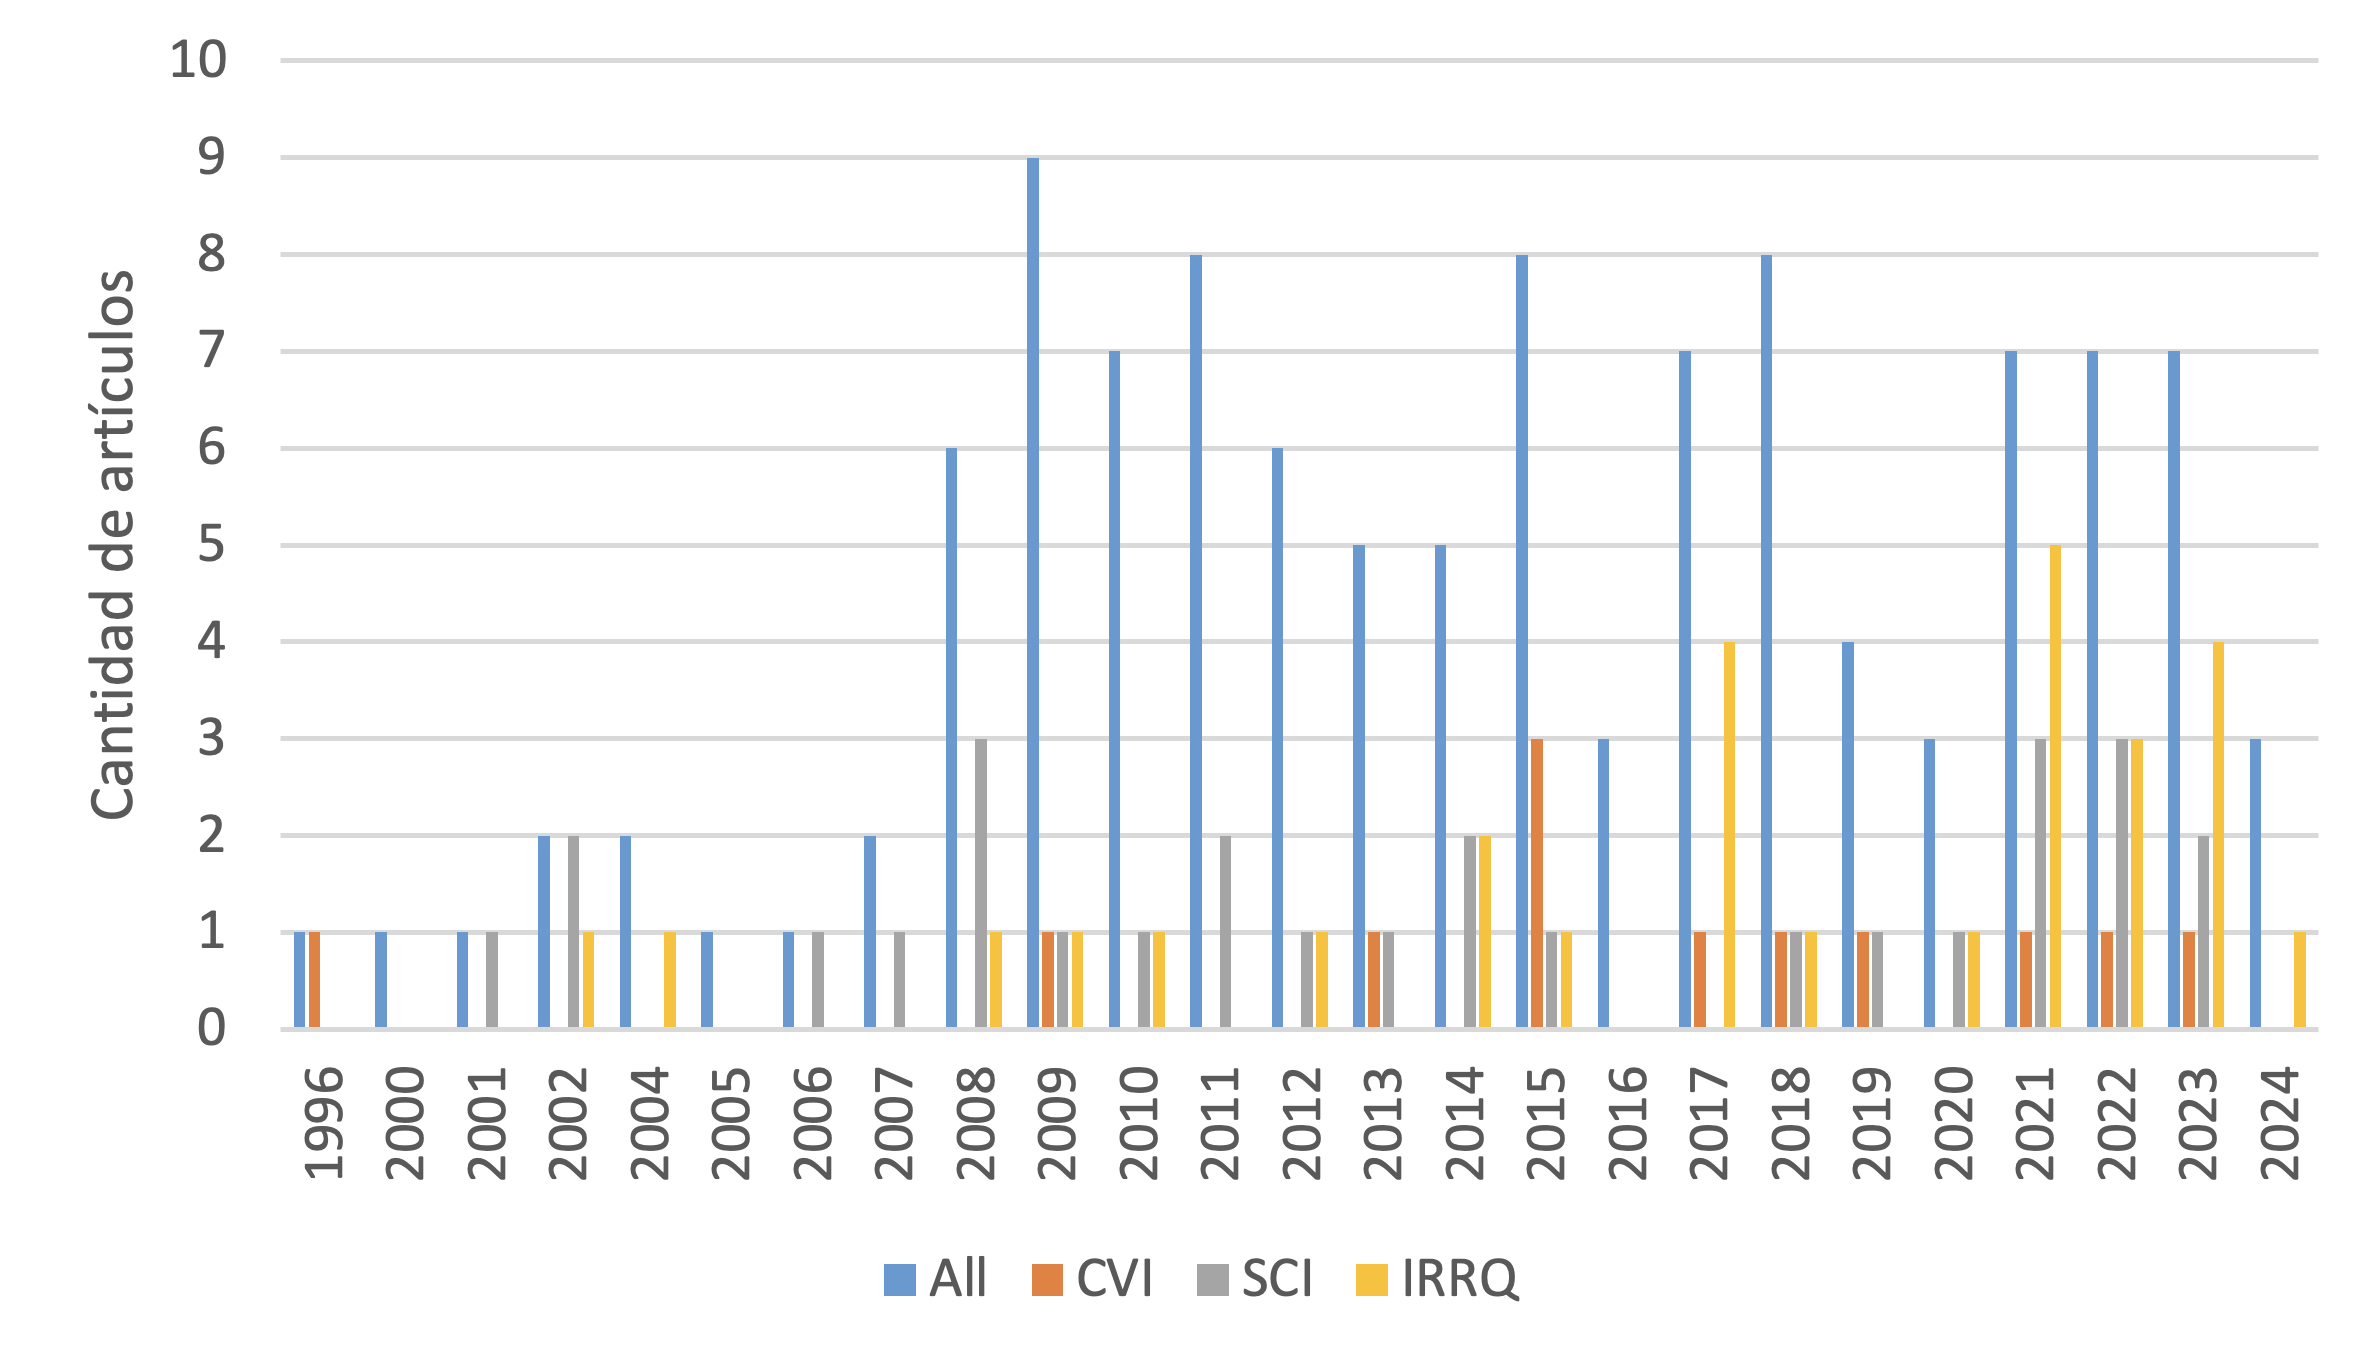
\includegraphics[width=0.95\textwidth]{tablas-images/sms/plot-freq-indices.png}
	\end{center}
	\caption{Cantidad de artículos en conformodidad con las métricas de calidad definidas en \ref{sec:priorizacionEstudios}}
	\label{fig:plot-anios-vs-indices-calidad}
\end{figure}



\subsection{Diferencias entre estrategias}

En la figura \ref{fig:plot-estrategia_vs_articulos} se pude apreciar la cantidad de artículos obtenido por cada

\begin{figure}[H]
	\centering
	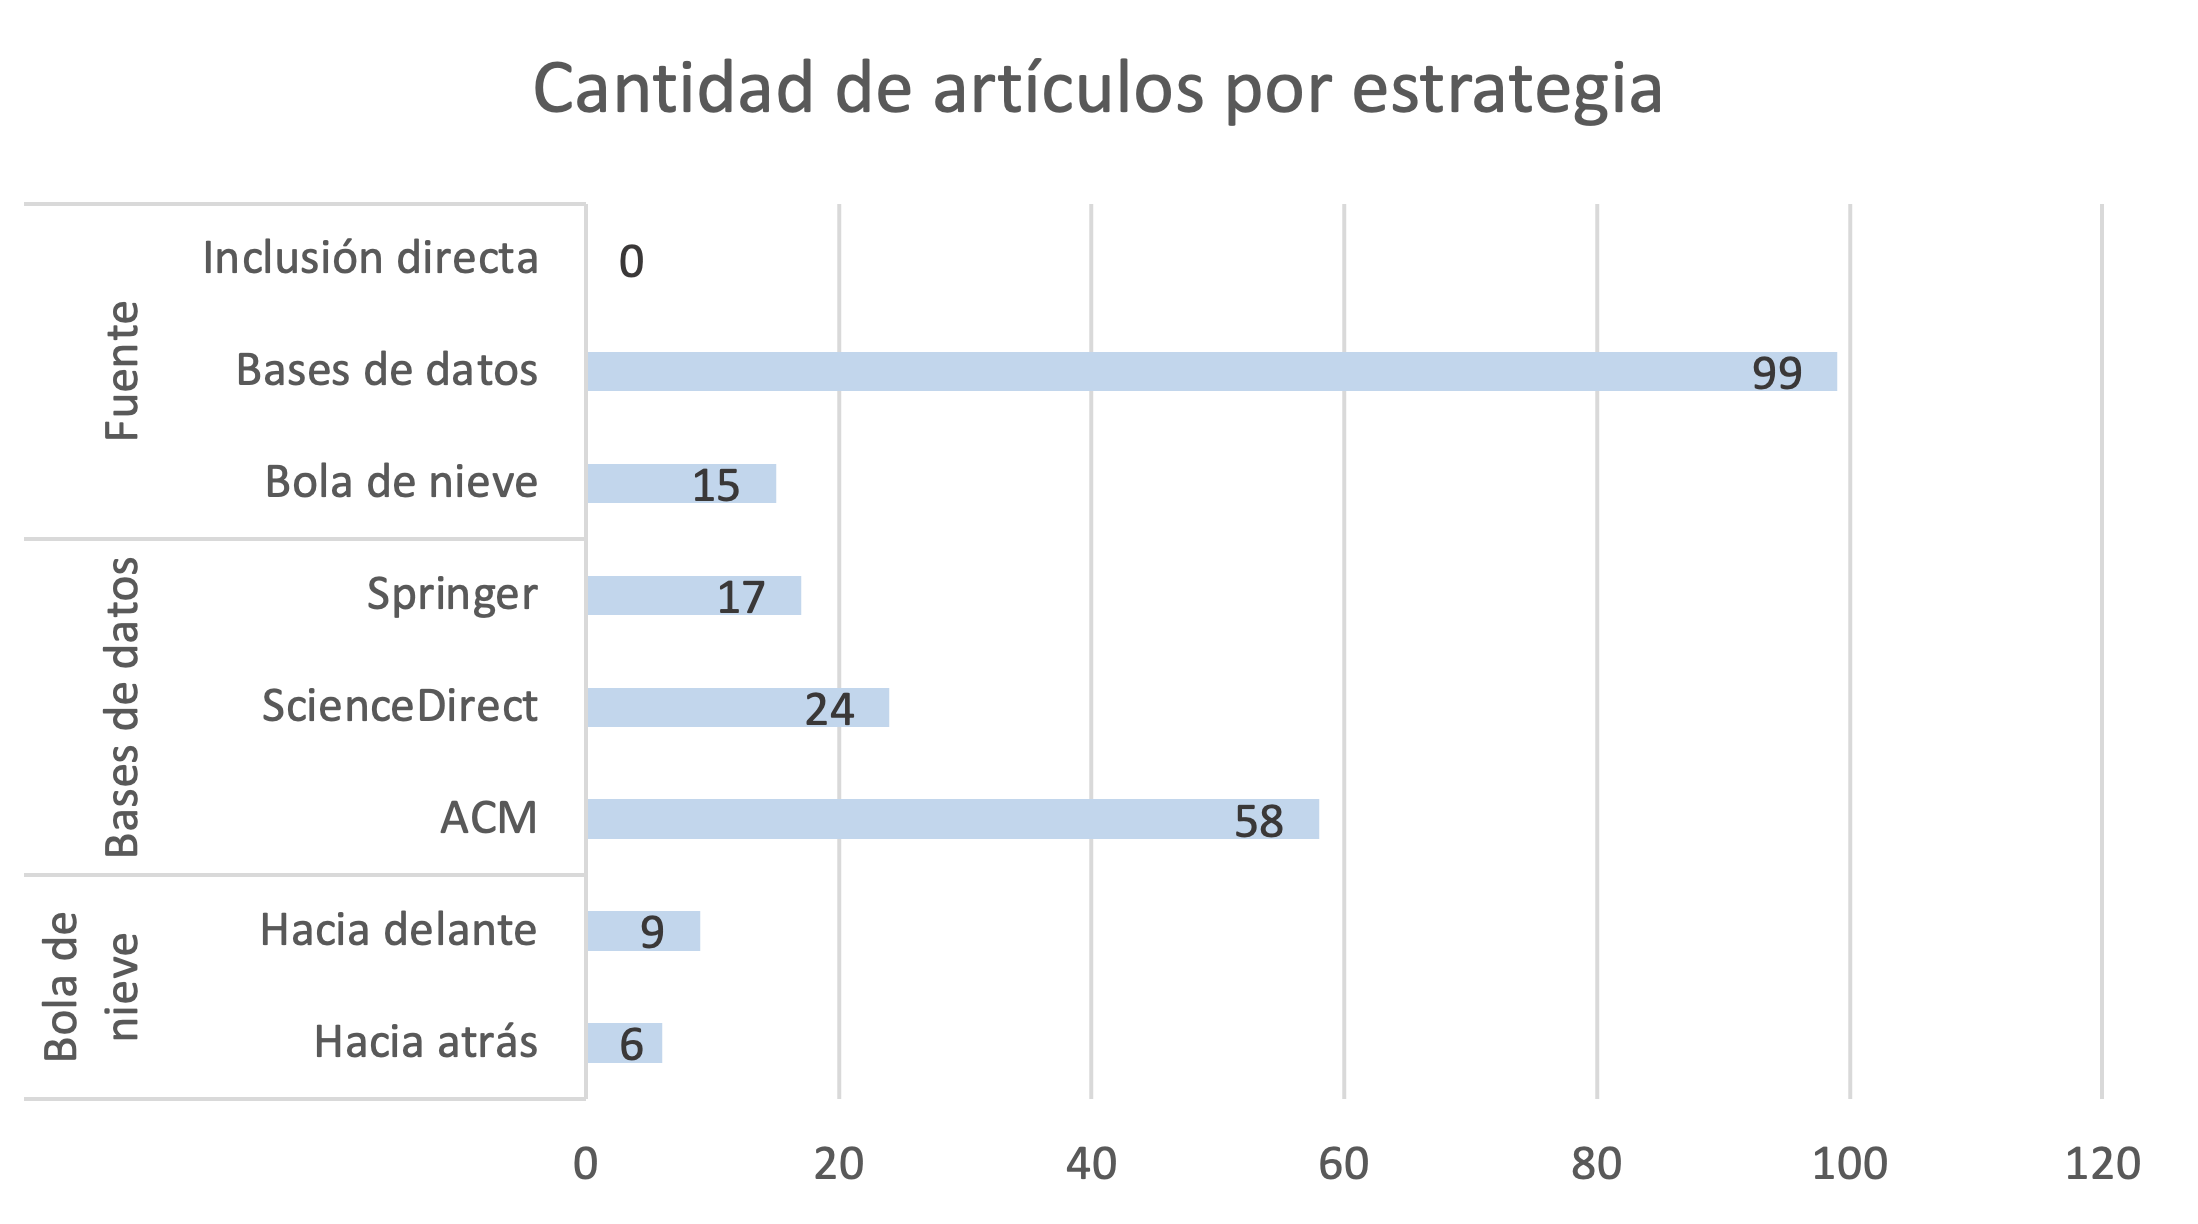
\includegraphics[scale=0.3] {tablas-images/sms/plot-estrategia_vs_articulos.png}
	\caption{Diagrama del proceso de eliminación de resultados}\label{fig:plot-estrategia_vs_articulos}
\end{figure}

\subsection{Tópicos frecuentes en los estudios}
\noindent

Del conjunto de 114 estudios analizados, se identificaron tópicos recurrentes mediante el análisis sistemático de los~\textit{abstracts} y~\textit{keywords} de cada publicación. Esta categorización temática reveló las áreas de investigación predominantes en el campo de estudio. Como se ilustra en la figura~\ref{fig:plot-topicos}, los tópicos más frecuentes incluyen \textbf{Grid Computing, \HPC, Cloud Computing, \HTC, y Parallel}, los cuales representan las tendencias principales en la literatura analizada.

\begin{figure}[H]
	\centering
	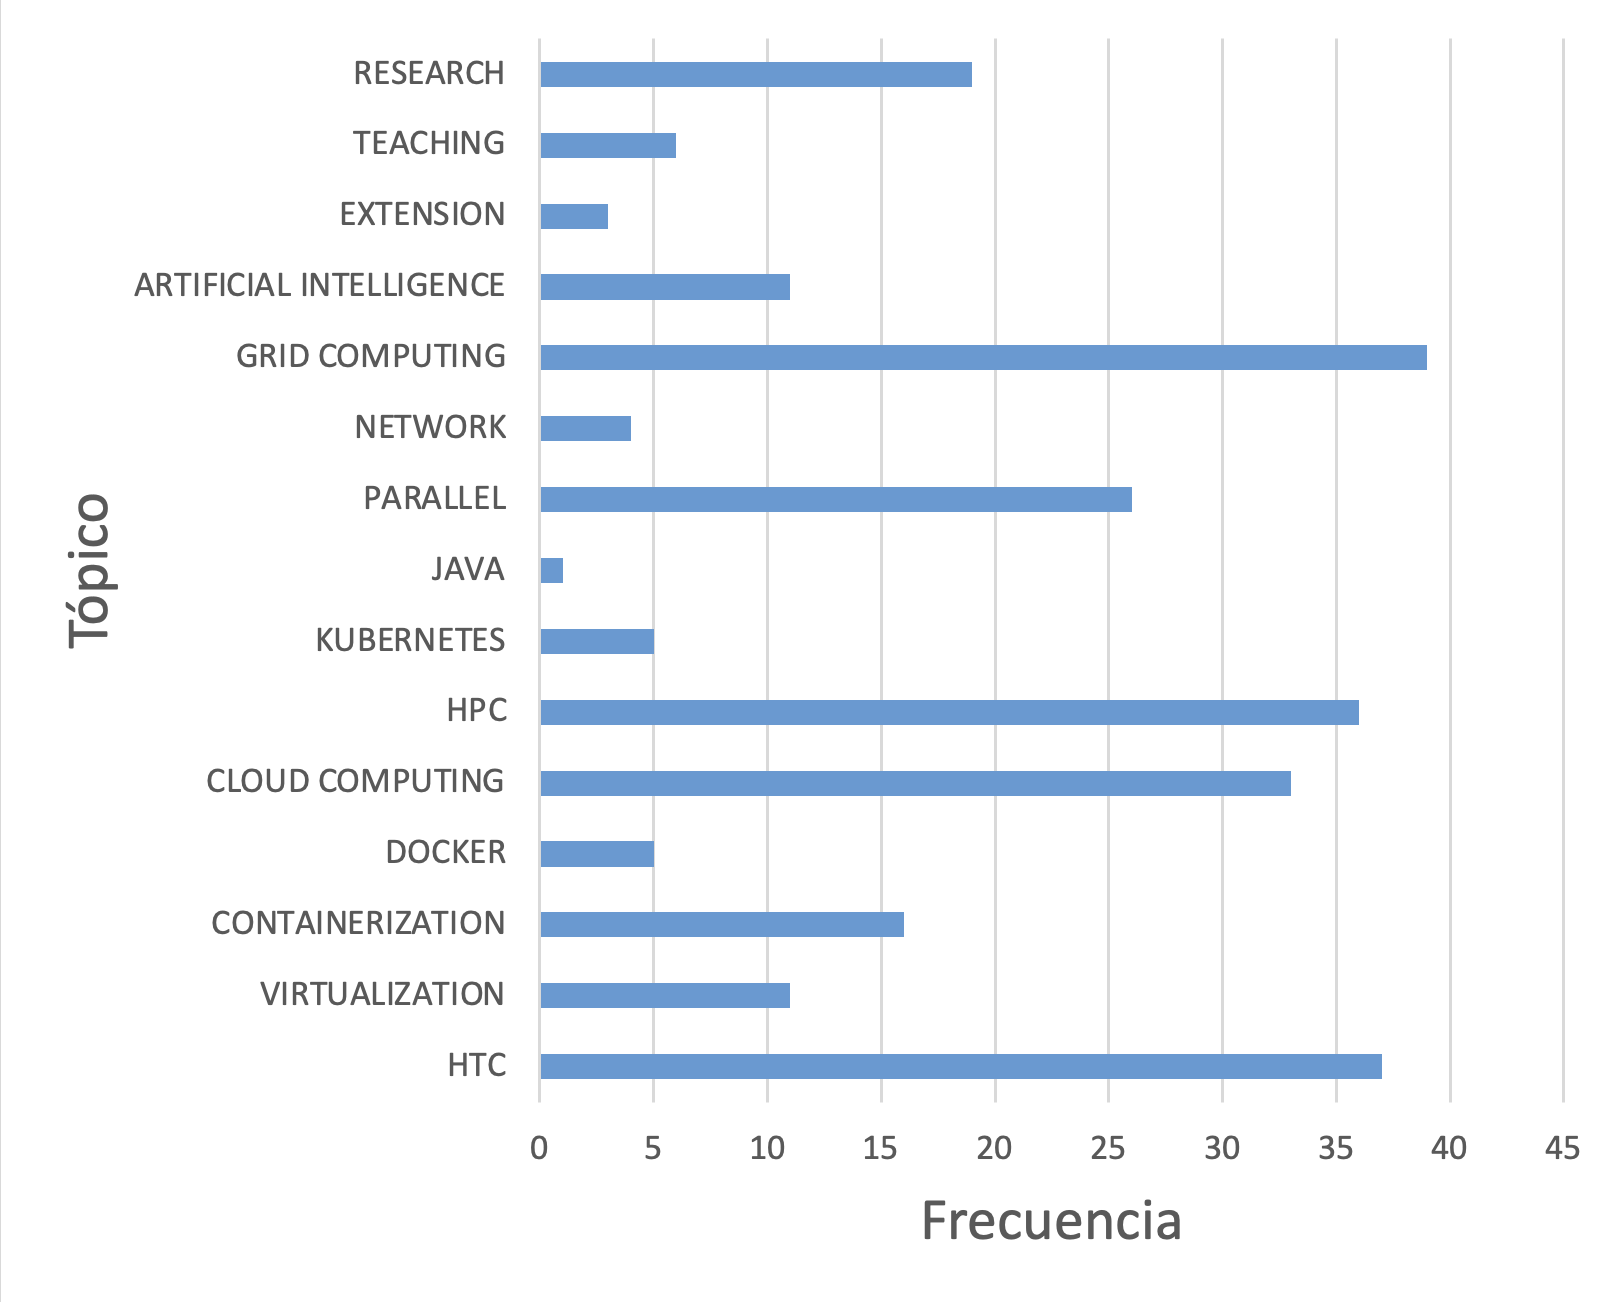
\includegraphics[scale=0.3] {tablas-images/sms/plot-topicos.png}
	\caption{Diagrama del proceso de eliminación de resultados}\label{fig:plot-topicos}
\end{figure}


\subsection{Conformidad con las preguntas de investigación}
Respecto al Cumplimiento con las preguntas de investigación (RQ) planteadas en la sección \ref{subsubsec:RQ-def}, todos los 114 estudios cumplían con la \textbf{RQ1}, mientras que únicamente 28 de estos cumplían con la \textbf{RQ2}. Ver figura \ref{fig:plot-venn-RQs}

\begin{figure}[H]
	\centering
	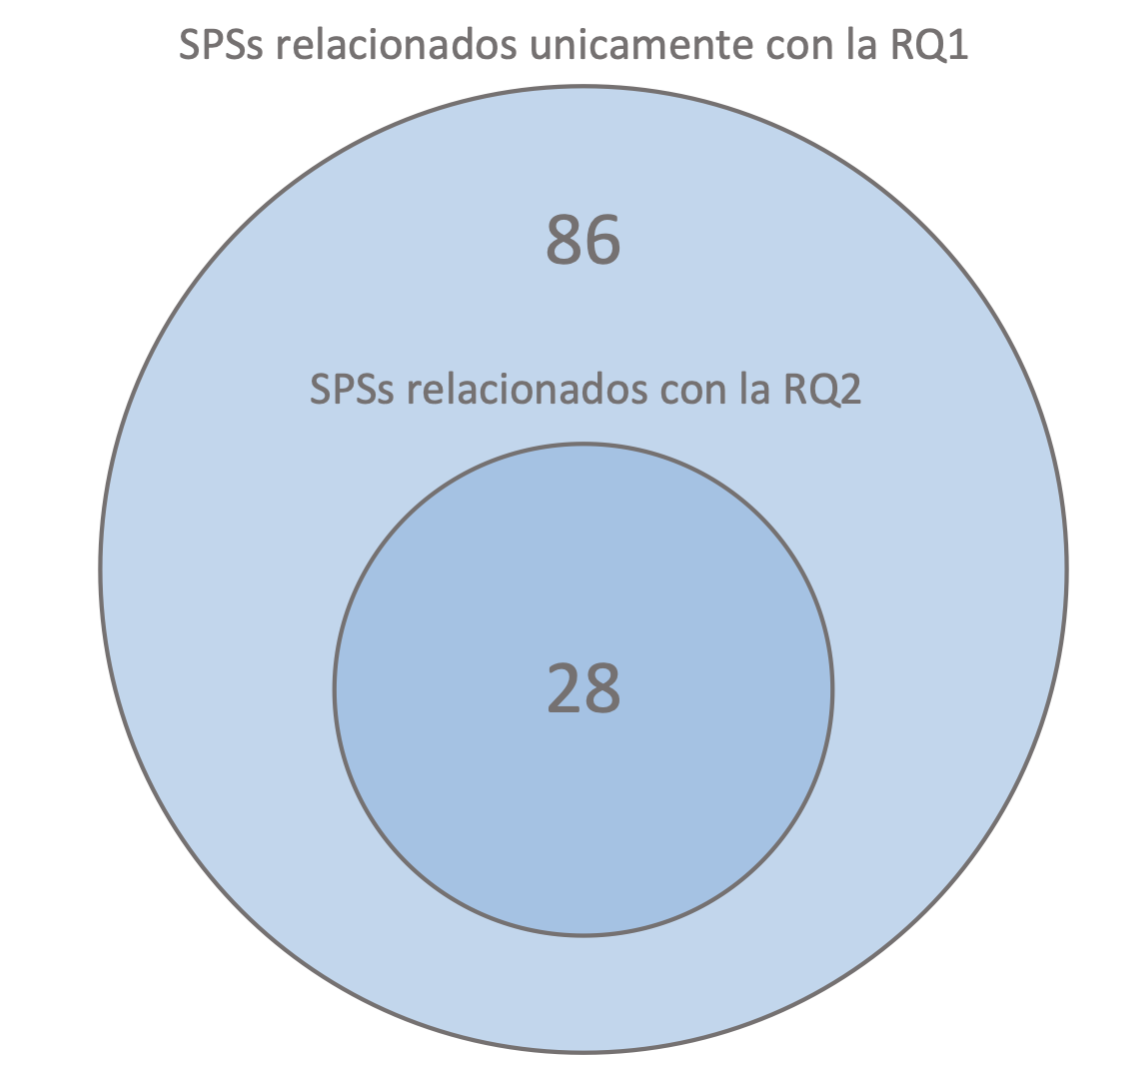
\includegraphics[scale=0.3] {tablas-images/sms/plot-venn-RQs.png}
	\caption{Diagrama del proceso de eliminación de resultados}\label{fig:plot-venn-RQs}
\end{figure}



\section{Información de la herramienta}

\noindent
La herramienta utilizada para este proceso de revisión de la literatura fue \textbf{SMS-BUILDER}, desarrollada por el Dr. Christian Andres Candela Uribe la cual se encuentra disponible en \textit{Docker Hub}. La imagen puede consultarse en el siguiente enlace:

\begin{center}
	\href{https://hub.docker.com/r/griduq/sms-builder}{\texttt{https://hub.docker.com/r/griduq/sms-builder}}
\end{center}



\section{Reproducibilidad del método}
\noindent
Con el fin de fomentar la reproducibilidad del método de revisión, se proporcionan dos mecanismos de verificación que permiten a los revisores y lectores acceder de forma transparente a la información utilizada, generada mediante la herramienta SMS-Builder de~\cite{SMSBuilder2020}
\begin{itemize}
	\item Un enlace de acceso público a la instancia de SMS-Builder que contiene todos los datos del proceso de revisión sistemática: \href{https://sms-htcondor.iti.grid.uniquindio.edu.co}{link}. Las credenciales de acceso son ``invitado'' tanto para el nombre de usuario como para la contraseña.
	\item Una imagen de Docker de acceso público que integra toda la documentación necesaria para crear un contenedor con los datos del proceso: \href{https://hub.docker.com/r/parritap/sms-htcondor-universes}{link}.
\end{itemize}

\noindent
Adicionalmente, se implementaron procesos de respaldo como medida de seguridad. Estos \textit{backups} fueron almacenados en ubicaciones diferentes, siguiendo la estrategia de respaldo \textbf{3--2--1}.



\section{Conclusiones de la revisión sistemática de la literatura}
\noindent
Esta revisión sistemática de la literatura sobre universos de HTCondor y tecnologías de computación distribuida de alto rendimiento logró identificar y analizar 114 estudios relevantes de un total inicial de 847 documentos recuperados de cinco bases de datos académicas principales. El proceso metodológico incluyó la aplicación de criterios de inclusión y exclusión que redujeron el corpus inicial en un 43.44\%, seguido de la eliminación de duplicados y la aplicación de estrategias complementarias como la búsqueda por bola de nieve. Los resultados revelan que la base de datos ACM fue la fuente más productiva con el 61.16\% de los artículos iniciales, mientras que IEEE y Taylor \& Francis no proporcionaron contribuciones significativas con las cadenas de búsqueda empleadas. El análisis temático identificó como tópicos predominantes \textbf{Grid Computing, HPC, Cloud Computing, HTC y Parallel}, evidenciando una concentración de la investigación en estas áreas específicas. Respecto al cumplimiento de las preguntas de investigación, todos los 114 estudios seleccionados respondieron a RQ1 (trabajos relacionados con universos de HTCondor en diversos dominios computacionales), mientras que solo 28 estudios (24.6\%) abordaron RQ2 (aplicaciones en funciones universitarias esenciales), lo que sugiere una brecha significativa en la literatura sobre la aplicación de estas tecnologías en contextos educativos y de extensión universitaria. La distribución temporal de las publicaciones y la diversidad de métricas de calidad aplicadas confirman la relevancia y actualidad del tema de investigación, proporcionando una base sólida para el desarrollo de taxonomías y marcos de trabajo en el dominio de HTCondor y computación distribuida.

\ChapterImageStar[cap:caracterizacionGRID]{Caracterización del GRID}{./images/fondo.png}\label{cap:caracterizacionGRID}
\mbox{}\\
\noindent
El Grupo de Investigación en Redes, Información y Distribución (\GRID) de la Universidad del Quindío se enmarca en los objetivos misionales de la institución: educación, investigación y extensión. Uno del los intereses particulares del \GRID es ofrecer servicios tecnológicos avanzados a la comunidad académica, con énfasis en los estudiantes de Ingeniería de Sistemas y Computación, quienes encuentran en este grupo un espacio de formación e innovación en temas de infraestructura, ingeniería de software y tecnologías emergentes.\\
La caracterización del \GRID\ resulta esencial para comprender su estructura, capacidades y necesidades en relación con la expansión de un nuevo universo HTCondor. A continuación, se presenta un análisis de los diferentes aspectos que definen el contexto institucional y tecnológico del grupo.

\section{Análisis de stakeholders del GRID}
\noindent
Con el fin de identificar los actores internos y externos que influyen en el desarrollo de las actividades del grupo, se realizó un análisis de \textit{stakeholders}. Este ejercicio permitió reconocer los diferentes intereses, roles y niveles de influencia que cada actor tiene en relación con la expansión de un nuevo universo HTCondor. Los principales \textit{stakeholders} identificados incluyen: investigadores del grupo, estudiantes de pregrado y posgrado, docentes de la Facultad de Ingeniería, y en un nivel más amplio, la comunidad académica de la Universidad del Quindío.
\\
\noindent
La tablaef{tab:stakeholders} presenta el análisis de los principales interesados en la expansión de los universos HTCondor dentro del contexto institucional. Se identifican actores internos y externos, especificando su rol, el tipo de relación con el proyecto, el nivel de impacto esperado, así como su poder de influencia, interés y compromiso frente a la iniciativa.

El análisis de interesados revela una estructura compleja de actores con distintos niveles de influencia y compromiso frente al proyecto. El Grupo de Investigación GRID emerge como el interesado crítico, concentrando simultáneamente el mayor impacto, poder de influencia, interés y compromiso. Esta posición central le otorga un rol determinante como beneficiario principal y tomador de decisiones, lo que subraya la necesidad de mantener una comunicación estrecha y continua con este grupo para asegurar la alineación del proyecto con sus expectativas estratégicas y operativas.

Los docentes de Ingeniería de Sistemas y los investigadores locales y externos constituyen el segundo nivel de importancia, caracterizándose por un alto interés en la solución y un potencial significativo como usuarios finales. Aunque su poder de decisión es limitado, su adopción efectiva de la tecnología será fundamental para validar el éxito del proyecto. Este segmento requiere especial atención en términos de usabilidad, documentación y capacitación, dado que su compromiso está condicionado a la utilidad práctica y los beneficios tangibles que puedan obtener. La diferencia principal entre ambos grupos radica en que los investigadores externos representarían el segmento de usuarios más activo e intensivo de la infraestructura.

El Programa de Ingeniería de Sistemas y Computación desempeña un rol estratégico como facilitador institucional con alto poder de influencia, particularmente en la provisión de recursos y la posibilidad de escalar la solución hacia otros programas académicos. Sin embargo, su compromiso relativamente bajo sugiere que será necesario demostrar claramente el valor estratégico e institucional del proyecto para asegurar su respaldo sostenido. Por otro lado, los estudiantes de pregrado presentan bajo impacto, poder e interés debido a la naturaleza especializada de la computación distribuida en el contexto académico de pregrado, lo que los posiciona como beneficiarios secundarios que validarán la solución más por uso ocasional que por dependencia operativa.

Finalmente, la comunidad HTCondor y los investigadores en HTC y HPC representan un interesado externo con una relación simbiótica particular: aunque no tienen poder de decisión sobre el proyecto y su compromiso es bajo, su rol como proveedores de conocimiento técnico es de alto impacto. La documentación y experiencias generadas por el proyecto podrían contribuir al fortalecimiento del ecosistema HTCondor, creando un valor agregado que trasciende los objetivos locales del proyecto. Esta relación sugiere la conveniencia de establecer canales de comunicación con esta comunidad para compartir hallazgos y mejores prácticas.

\begin{table}[H]
	\centering
	\fontsize{7}{7}\selectfont % Cambia el primer número (9) al tamaño deseado, el segundo es el interlineado
	\setlength{\tabcolsep}{3pt} % reduce el espacio horizontal entre columnas
	\renewcommand{\arraystretch}{1.4} % espacio entre filas
	\begin{tabularx}{\textwidth}{%
		>{\raggedright\arraybackslash}p{1.7cm}  % Columna 1: Interesado
		>{\raggedright\arraybackslash}p{1.5cm}    % Columna 2: Rol
		>{\raggedright\arraybackslash}p{2.3cm}  % Columna 3: Relación
		>{\raggedright\arraybackslash}p{1.4cm}  % Columna 4: Impacto
		>{\raggedright\arraybackslash}p{2.0cm}  % Columna 5: Poder de influencia
		>{\raggedright\arraybackslash}p{2.5cm}    % Columna 6: Interés
		>{\raggedright\arraybackslash}p{2.0cm}} % Columna 7: Compromiso
		\toprule
		\textbf{Interesado}                              & \textbf{Rol}                               & \textbf{Relación}                                                                                                                                      & \textbf{Impacto} & \textbf{Poder de influencia}                                                                                            & \textbf{Interés}                                                                                                                          & \textbf{Compromiso}                                                                                \\
		\midrule
		Docentes de Ingeniería de Sistemas               & Usuarios clave                             & Utilizarán los entregables del proyecto en actividades de enseñanza e investigación                                                                    & Medio-Alto       & Medio, pueden proponer mejoras pero no tienen poder de decisión sobre la implementación                                 & Medio-Alto, requieren soliuciones tecnológicas para integrarlas en procesos académicos e investigativos                                   & Medio, condicionado a la utilidad práctica y aplicabilidad de la solución                          \\
		\midrule
		Estudiantes de Ingeniería de Sistemas            & Beneficiarios potenciales                  & Podrían utilizar la infraestructura en proyectos académicos y acceder a información sobre el estudio                                                   & Bajo             & Bajo, carecen de poder de decisión aunque su adopción validará la efectividad de la solución                            & Bajo, dado que la computación distribuida es un área especializada con uso poco frecuente en el contexto académico general                & Bajo                                                                                               \\
		\midrule
		Grupo de Investigación GRID                      & Beneficiario principal                     & Proporciona la infraestructura base, evalúa la solución propuesta y mide su impacto                                                                    & Alto             & Alto, tiene autoridad para decidir la adopción e implementación de la tecnología                                        & Alto, busca optimizar sus servicios y fortalecer su posicionamiento en el ámbito de la investigación y la colaboración interuniversitaria & Alto, la solución potenciará directamente sus capacidades de infraestructura                       \\
		\midrule
		Grupos de Investigación Locales y Externos       & Beneficiarios principales                  & Identificarían oportunidades significativas para potenciar sus líneas de investigación                                                                 & Medio            & Medio-Bajo, pueden influir mediante solicitudes específicas de funcionalidades o mejoras                                & Alto, la solución podría reducir significativamente los tiempos de procesamiento y obtención de resultados en sus proyectos               & Medio-Alto, conformarían uno de los segmentos principales de usuarios finales                      \\
		\midrule
		Programa de Ingeniería de Sistemas y Computación & Facilitador institucional                  & Puede proveer respaldo institucional, recursos y normativas que faciliten la adopción                                                                  & Alto             & Alto, posee autoridad para aprobar asignación de recursos e invitar a otros programas académicos a utilizar la solución & Medio, su interés se centra en aspectos institucionales y estratégicos más que operativos                                                 & Bajo-Medio, especialmente si la solución no impacta directamente sus procesos de gestión académica \\
		\midrule
		Comunidad HTCondor e investigadores en HTC y HPC & Proveedores y consumidores de conocimiento & Suministran documentación técnica esencial para la implementación y se benefician de la documentación generada a partir de la experiencia del proyecto & Alto             & Bajo, no participan en decisiones sobre el proyecto                                                                     & Bajo-Medio, la implementación exitosa fortalecería la adopción de HTCondor y ampliaría el impacto de la tecnología                        & Bajo, sujeto a la alineación de resultados con sus objetivos comunitarios                          \\
		\bottomrule
	\end{tabularx}
	\caption{Análisis de stakeholders}\label{tab:stakeholders}
\end{table}


\section{Priorización de stakeholders}
Una vez realizada la identificación de los \textit{stakeholders}, se emprendió un proceso de priorización para determinar cuáles poseen mayor impacto y poder de decisión en el proyecto. Esta clasificación resulta crucial para establecer estrategias de comunicación, gestión de expectativas y participación activa en la definición de requerimientos. De esta manera, se busca que los actores más influyentes en la toma de decisiones y en la adopción tecnológica sean atendidos de forma prioritaria, aumentando las probabilidades de éxito en la implementación.

\begin{figure}[H]
    \centering
    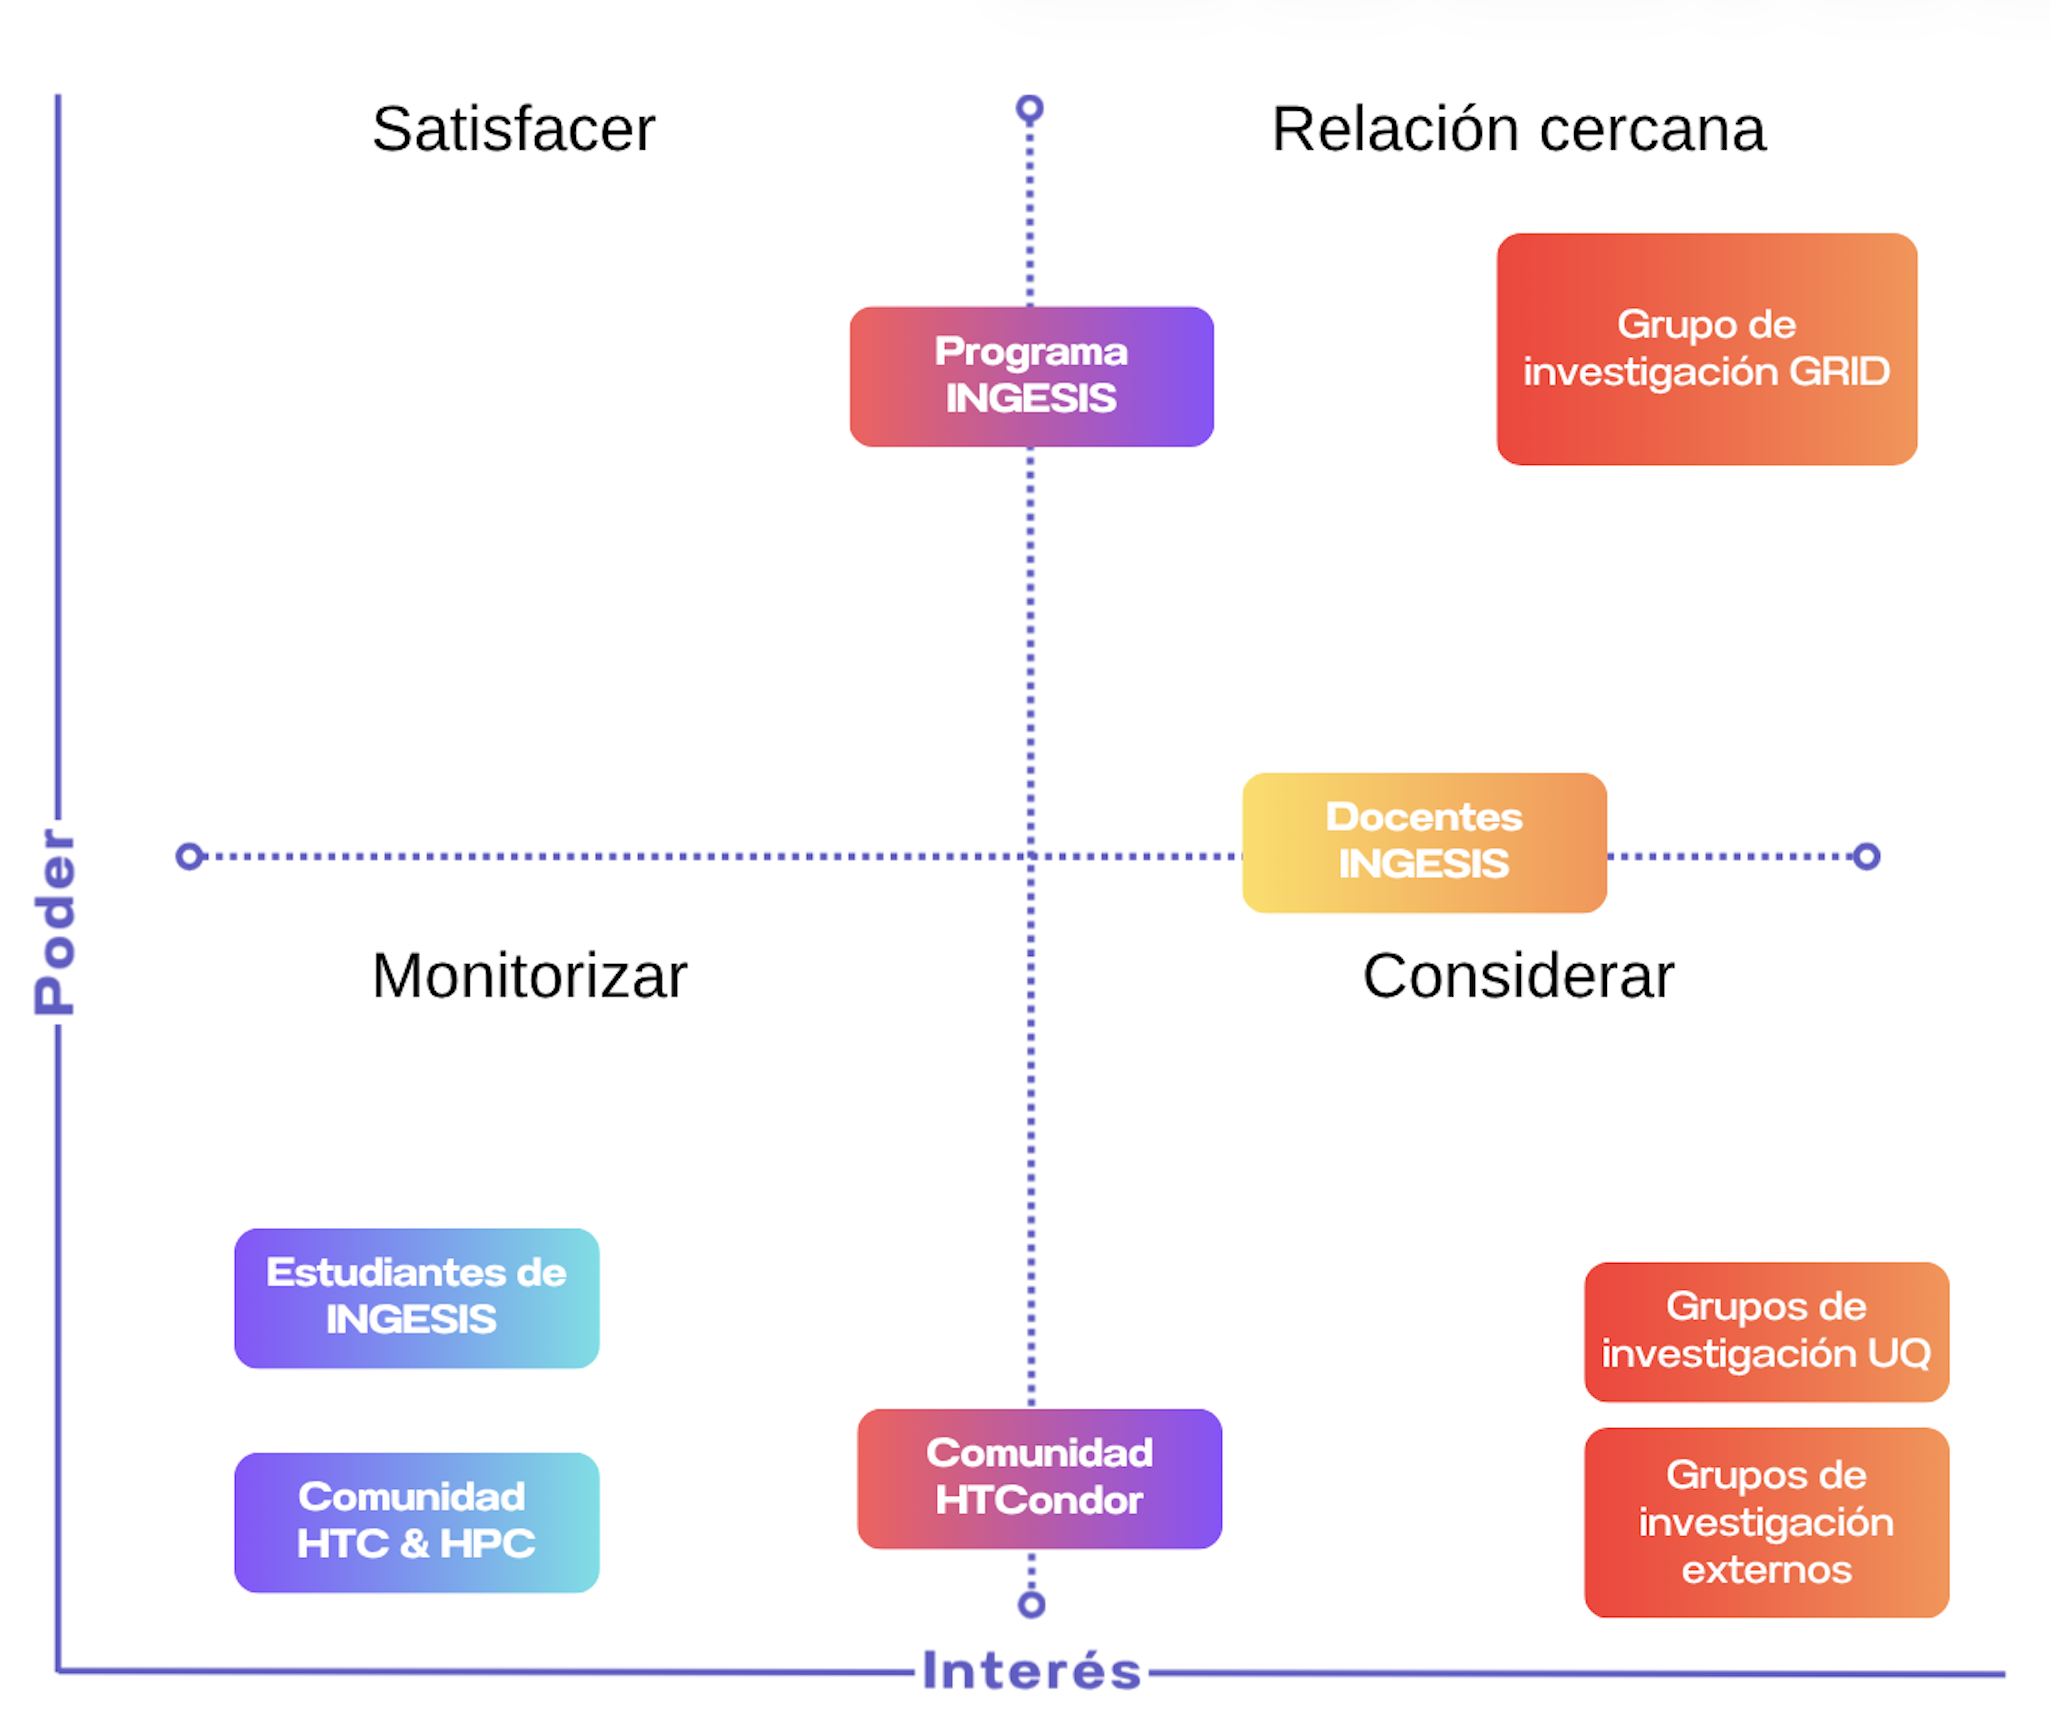
\includegraphics[width=\textwidth] {tablas-images/cp1/priorizacionStakeholders.png}
    \caption{Priorización de stakeholders del proyecto}\label{fig:tabla-priorizacion-stakeholders}
\end{figure}

\section{Integrantes y áreas de trabajo del GRID}
El \GRID\ está conformado por un equipo multidisciplinario de investigadores y profesionales que, desde sus diferentes áreas de experticia, contribuyen al avance en campos como computación de alto rendimiento, \textit{big data}, inteligencia artificial, redes de computadoras y desarrollo de software. A continuación, se presenta una lista de los integrantes actuales del grupo, junto con sus respectivas líneas de trabajo y áreas de especialización:
\begin{itemize}
	\item \href{https://scienti.minciencias.gov.co/cvlac/visualizador/generarCurriculoCv.do?cod_rh=0000210897}{\underline{{\textbf{Christian Andrés Candela Uribe}}}}: Microservicios, desarrollo de software, minería de datos, infraestructura TI.\@
	\item \href{https://scienti.minciencias.gov.co/cvlac/visualizador/generarCurriculoCv.do?cod_rh=0001383939}{\underline{{\textbf{Luis Eduardo Sepúlveda Rodríguez}}}}: Infraestructura de TI, HPC, computación paralela.
	\item \href{https://scienti.minciencias.gov.co/cvlac/visualizador/generarCurriculoCv.do?cod_rh=0001638854}{\underline{{\textbf{Carlos Andrés Flórez Villarraga}}}}: Programación y algoritmia, inteligencia artificial.
	\item \href{https://scienti.minciencias.gov.co/cvlac/visualizador/generarCurriculoCv.do?cod_rh=0001343801}{\underline{{\textbf{Carlos Eduardo Gómez Montoya}}}}: Redes, ingeniería de software, cloud computing.
	\item \href{https://scienti.minciencias.gov.co/cvlac/visualizador/generarCurriculoCv.do?cod_rh=0001398775}{\underline{{\textbf{Sergio Augusto Cardona Torres}}}}: Big data y análisis de datos, ingeniería de software, sistemas adaptativos, informática educativa.
	\item \href{https://scienti.minciencias.gov.co/cvlac/visualizador/generarCurriculoCv.do?cod_rh=0000193550}{\underline{{\textbf{Sonia Jaramillo Valbuena}}}}: Big data, electroquímica, inteligencia artificial.
	\item \href{https://scienti.minciencias.gov.co/cvlac/visualizador/generarCurriculoCv.do?cod_rh=0000283495}{\underline{{\textbf{Julián Esteban Gutiérrez Posada}}}}: Microservicios, desarrollo de software, minería de datos, infraestructura TI, HPC, computación paralela, redes, ingeniería de software.
\end{itemize}

La diversidad de líneas de trabajo de los integrantes fortalece la capacidad del grupo para abordar proyectos de carácter transversal y multidisciplinario, lo cual resulta particularmente relevante para el diseño e implementación de soluciones arquitectónicas soportadas en tecnologías de virtualización.

\section{Misión del GRID}
La misión del GRID es heredada de la Universidad del Quindío. A continuación se presenta la misión del GRID:\@

\begin{quote}
	\textit{La Universidad del Quindío contribuye a la transformación de la sociedad, mediante la formación integral desde el ser, el saber y el hacer, de líderes reflexivos y gestores del cambio; con estándares de calidad, a través de una oferta de formación en diferentes metodologías, que responda a una sociedad basada en el conocimiento; una investigación pertinente, que aporte a la solución de las problemáticas del desarrollo e integrada con la extensión y proyección social; educando en tiempos del posconflicto y de la consolidación de la paz, apoyada en una gestión creativa y con estándares de calidad.}
\end{quote}

A partir de esta misión, se identifican los siguientes pilares fundamentales:

\begin{itemize}
	\item \textbf{Docencia:} La Universidad del Quindío contribuye a la transformación de la sociedad, mediante la formación integral desde el ser, el saber y el hacer, de líderes reflexivos y gestores del cambio; con estándares de calidad, a través de una oferta de formación en diferentes metodologías, que responda a una sociedad basada en el conocimiento.

	\item \textbf{Investigación:} Una investigación pertinente, que aporte a la solución de las problemáticas del desarrollo e integrada con la extensión y proyección social.

	\item \textbf{Extensión y Desarrollo Social:} Apoyada en una gestión creativa y con estándares de calidad.

	\item \textbf{Responsabilidad Social:} Educando en tiempos del posconflicto y de la consolidación de la paz.
\end{itemize}

\section{Visión del GRID}
La misión de la Universidad del Quindío se complementa con su visión institucional, la cual también es adoptada por el \GRID. A continuación se presenta la visión del \GRID:\@

\begin{quote}
	\textit{En el año 2025, la Universidad del Quindío estará consolidada como una institución \textit{Pertinente --- Creativa --- Integradora}, acreditada de alta calidad, con reconocimiento nacional e internacional en sus procesos de formación a través de diferentes metodologías, de investigación, extensión, proyección y responsabilidad social.}
\end{quote}

A partir de esta visión, se destacan los siguientes enfoques estratégicos:

\begin{itemize}
	\item \textbf{Gestión:} La Universidad del Quindío estará consolidada como una institución \textit{Pertinente --- Creativa --- Integradora}.

	\item \textbf{Docencia:} Acreditada de alta calidad en sus procesos de formación a través de diferentes metodologías.

	\item \textbf{Investigación:} Consolidada como pertinente y de alta calidad en sus procesos de investigación.

	\item \textbf{Extensión y Desarrollo Social:} Procesos creativos e integradores en proyección social.

	\item \textbf{Responsabilidad Social:} Reconocimientos en sus procesos de responsabilidad social.
\end{itemize}

\section{Impacto del proyecto en el GRID}
La ampliación de la infraestructura HTCondor mediante la incorporación de un nuevo universo representa un impacto estratégico multidimensional para el Grupo de Investigación GRID. Este proyecto constituye un avance decisivo en la consolidación de una infraestructura de computación distribuida más amplia y capaz, lo que incrementa la competitividad del \GRID en el ámbito de la computación distribuida y de alta productividad. Además, esta expansión podría ayudar a fortalecer el posicionamiento del grupo como referente regional en tecnologías HTC y potenciar su capacidad para establecer colaboraciones interuniversitarias tanto a nivel nacional como internacional.


%%%%% ##############################################################################################################################
%%%%% ##############################################################################################################################
%%%%% ##############################################################################################################################
%%%%% #############################################################################################################################


\section{Caracterización de la infraestructura de computación distribuida del GRID}
\noindent
En la presente sección se especificarán las características técnicas actuales de la infraestructura de computación distribuida HTCondor del grupo \GRID.


% !TODO Verificar el conteo real de la máquinas.
\subsection{Clúster de máquinas Raspberry-Pi}
\noindent

Actualmente, el grupo \GRID cuenta con un clúster compuesto por computadoras Raspberry Pi, distribuidas en nueve torres identificadas como \textbf{Torre 1} a \textbf{Torre 9}. Cada torre contiene siete equipos, con excepción de la Torre 1, que posee únicamente dos: uno opera como nodo maestro y el otro como nodo de envío de tareas. Los equipos restantes de las demás torres funcionan como nodos ejecutores.
\\
Si bien el \GRID posee nueve torres de equipos Raspberry-Pi, la torre novena se encuentra en funcionamiento. \\
%# Tablas de caracterización del GRID 

\begin{table}[h]
	\centering
	\begin{tabular}{|p{6cm}|p{8cm}|}
		\hline
		\multicolumn{2}{|c|}{\textbf{Características las máquinas Raspberry Pi del clúster HTCondor}} \\
		\hline
		Modelo                   & Raspberry Pi 3 Modelo B                                            \\
		\hline
		Versión                  & 1.2                                                                \\
		\hline
		CPU                      & ARMv7 de 1.2GHz                                                    \\
		\hline
		RAM                      & 1 GB                                                               \\
		\hline
		Cantidad de Procesadores & 4                                                                  \\
		\hline
		Sistema Operativo        & Raspbian GNU/Linux 9.1 (stretch) armv7l                            \\
		\hline
		Ubicación                & Oficina tercer piso                                                \\
		\hline
	\end{tabular}
	\caption{Especificaciones de la computadoras Raspberry Pi de GRID}
	\label{table:raspberries-pi-specs}
\end{table}





% Tabla con especificacioens de técnicas de las Raspberry-Pi
En la tabla \ref{table:raspberries-pi-specs} se pueden evidenciar las especificaciones técnicas de las máquinas disponibles para la infraestructura HTCondor del \GRID.
\\


%%#################################  FOTOS TORRES  #########################################
%Image de las Raspberry-Pi
\begin{figure}[H]
	\centering
	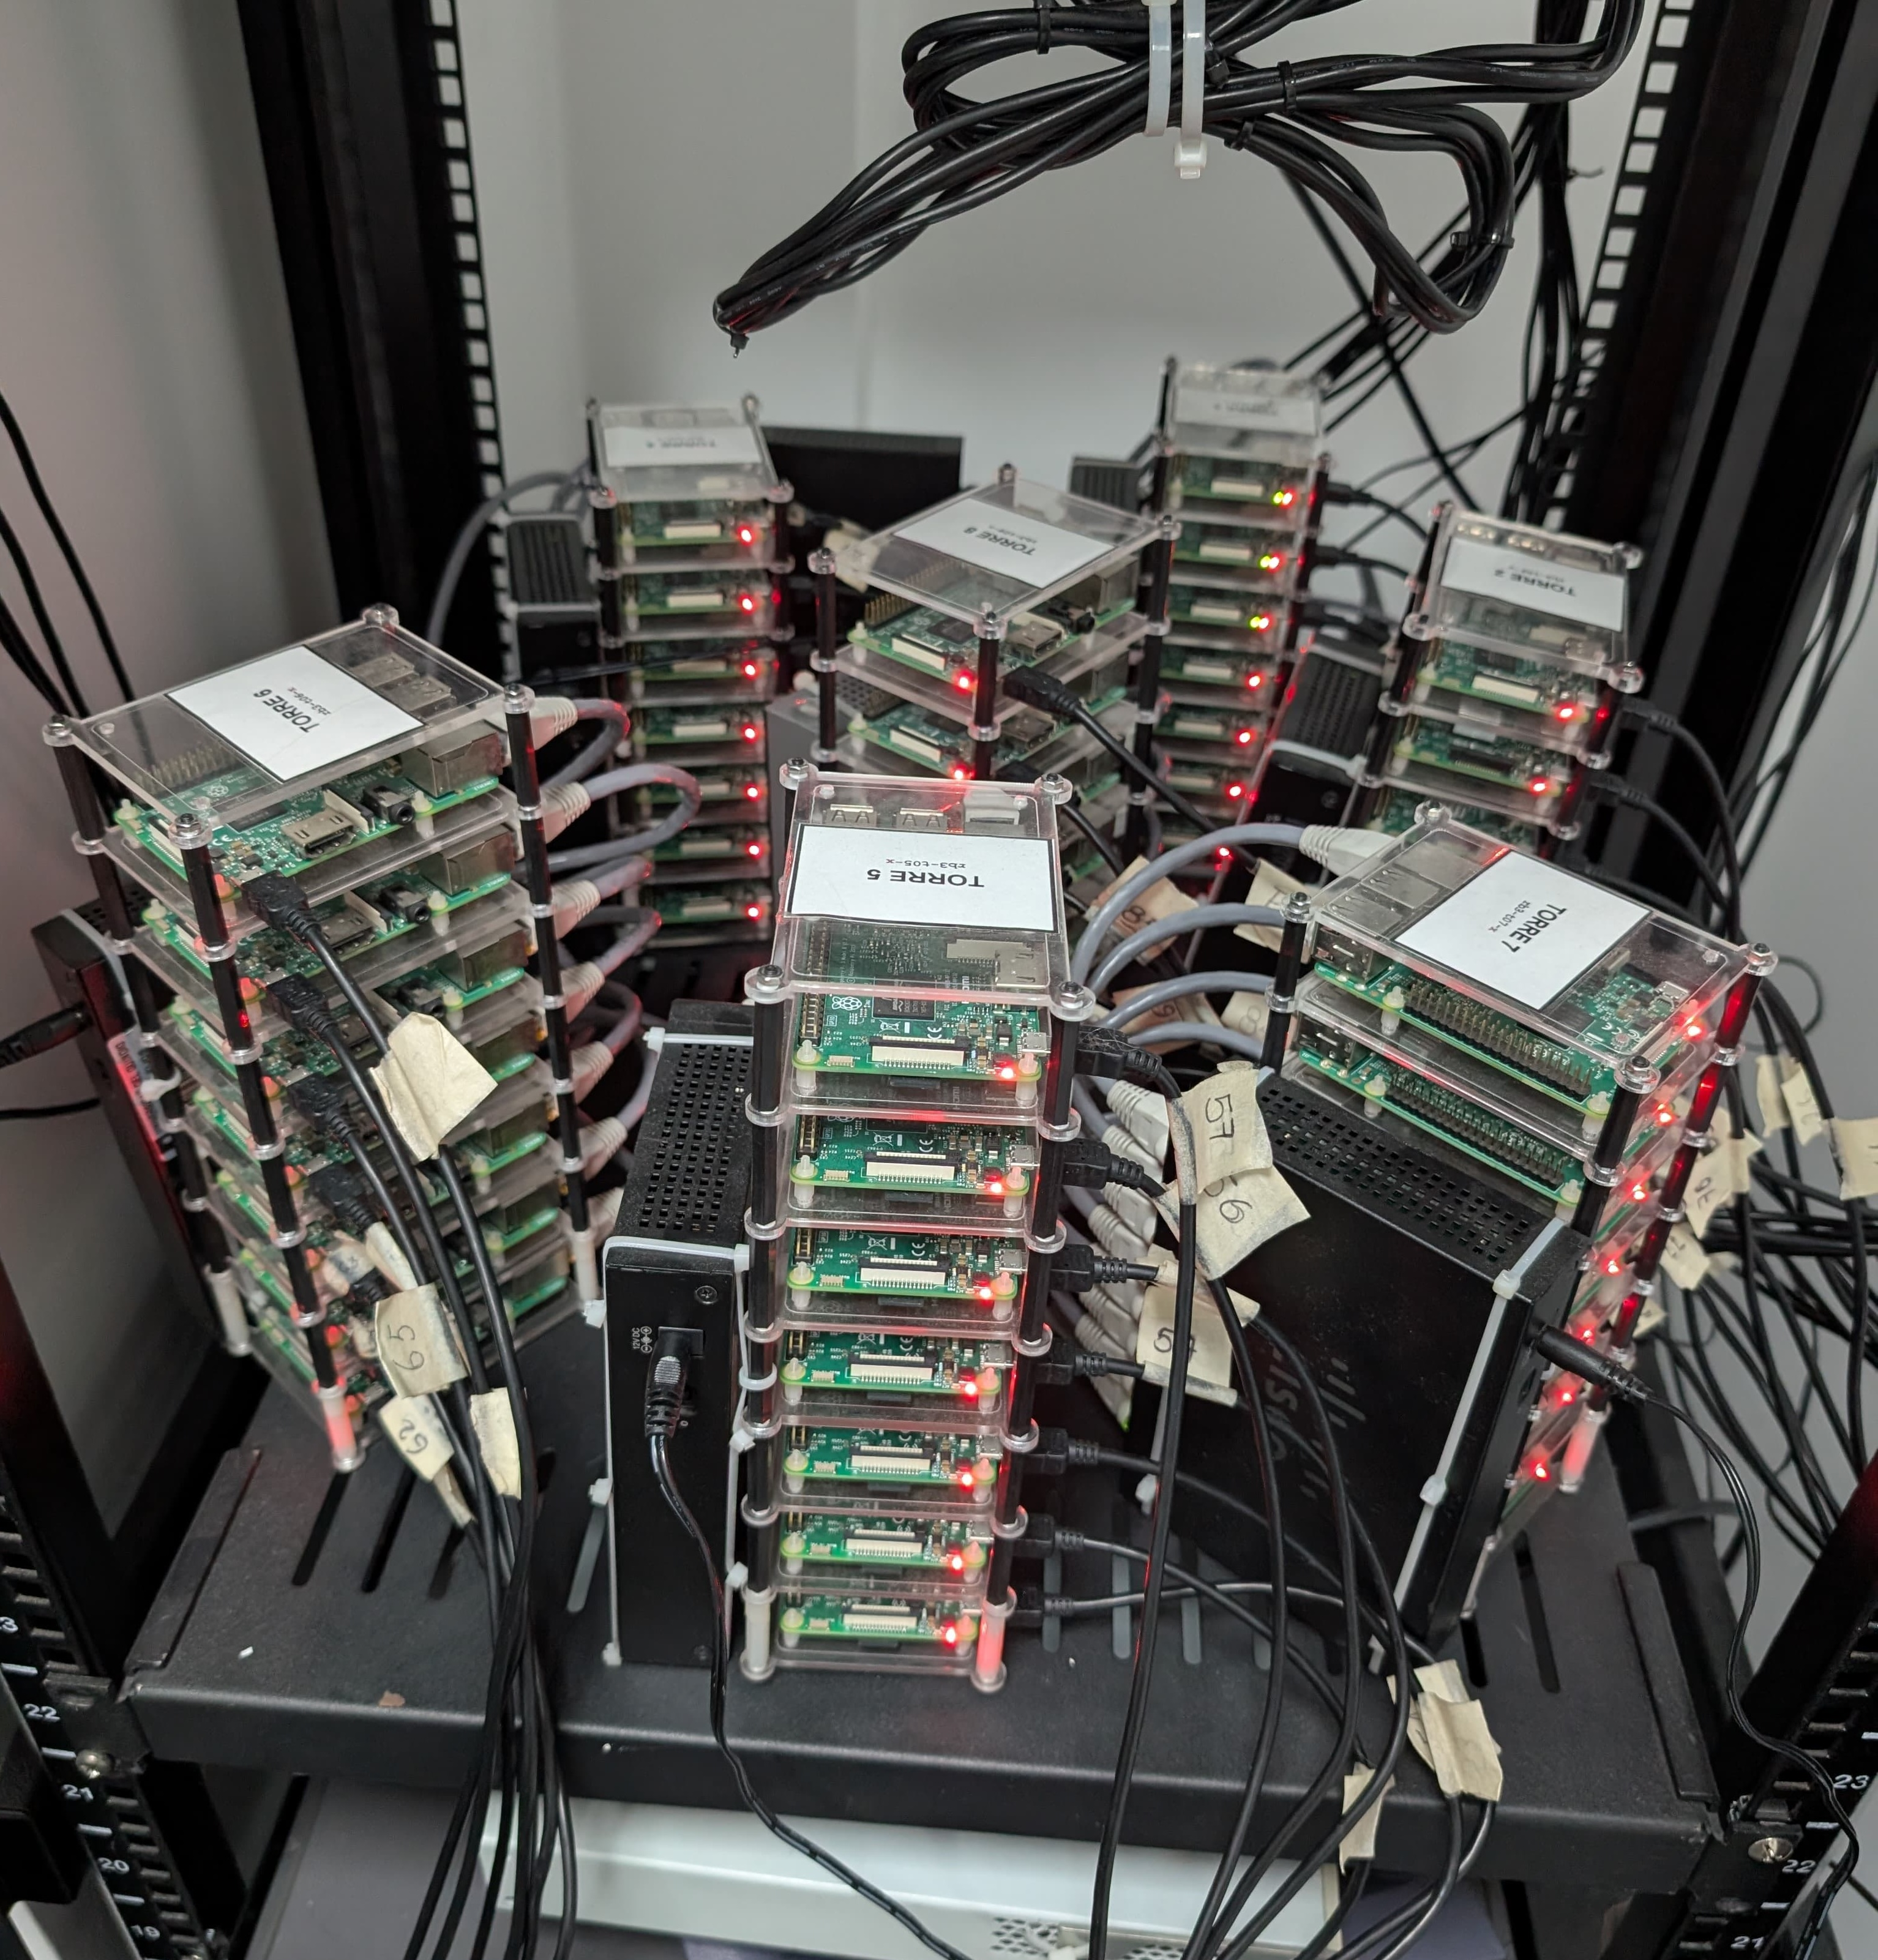
\includegraphics[scale=0.07]{tablas-images/raspberries/torres-raspberries.jpg}
	\caption{Vista general de las maquinas Raspberry-Pi}
	\label{fig:foto-torres-rasp}
\end{figure}


\noindent
En la figura \ref{fig:foto-torres-rasp} se muestra la imagen de las siete torres de Raspberry-Pi localizadas en la oficina del tercer piso de ingeniería. A continuación se muestran las demás torres individualmente.


%Torre BINARIA
\begin{figure}[H]
	\centering
	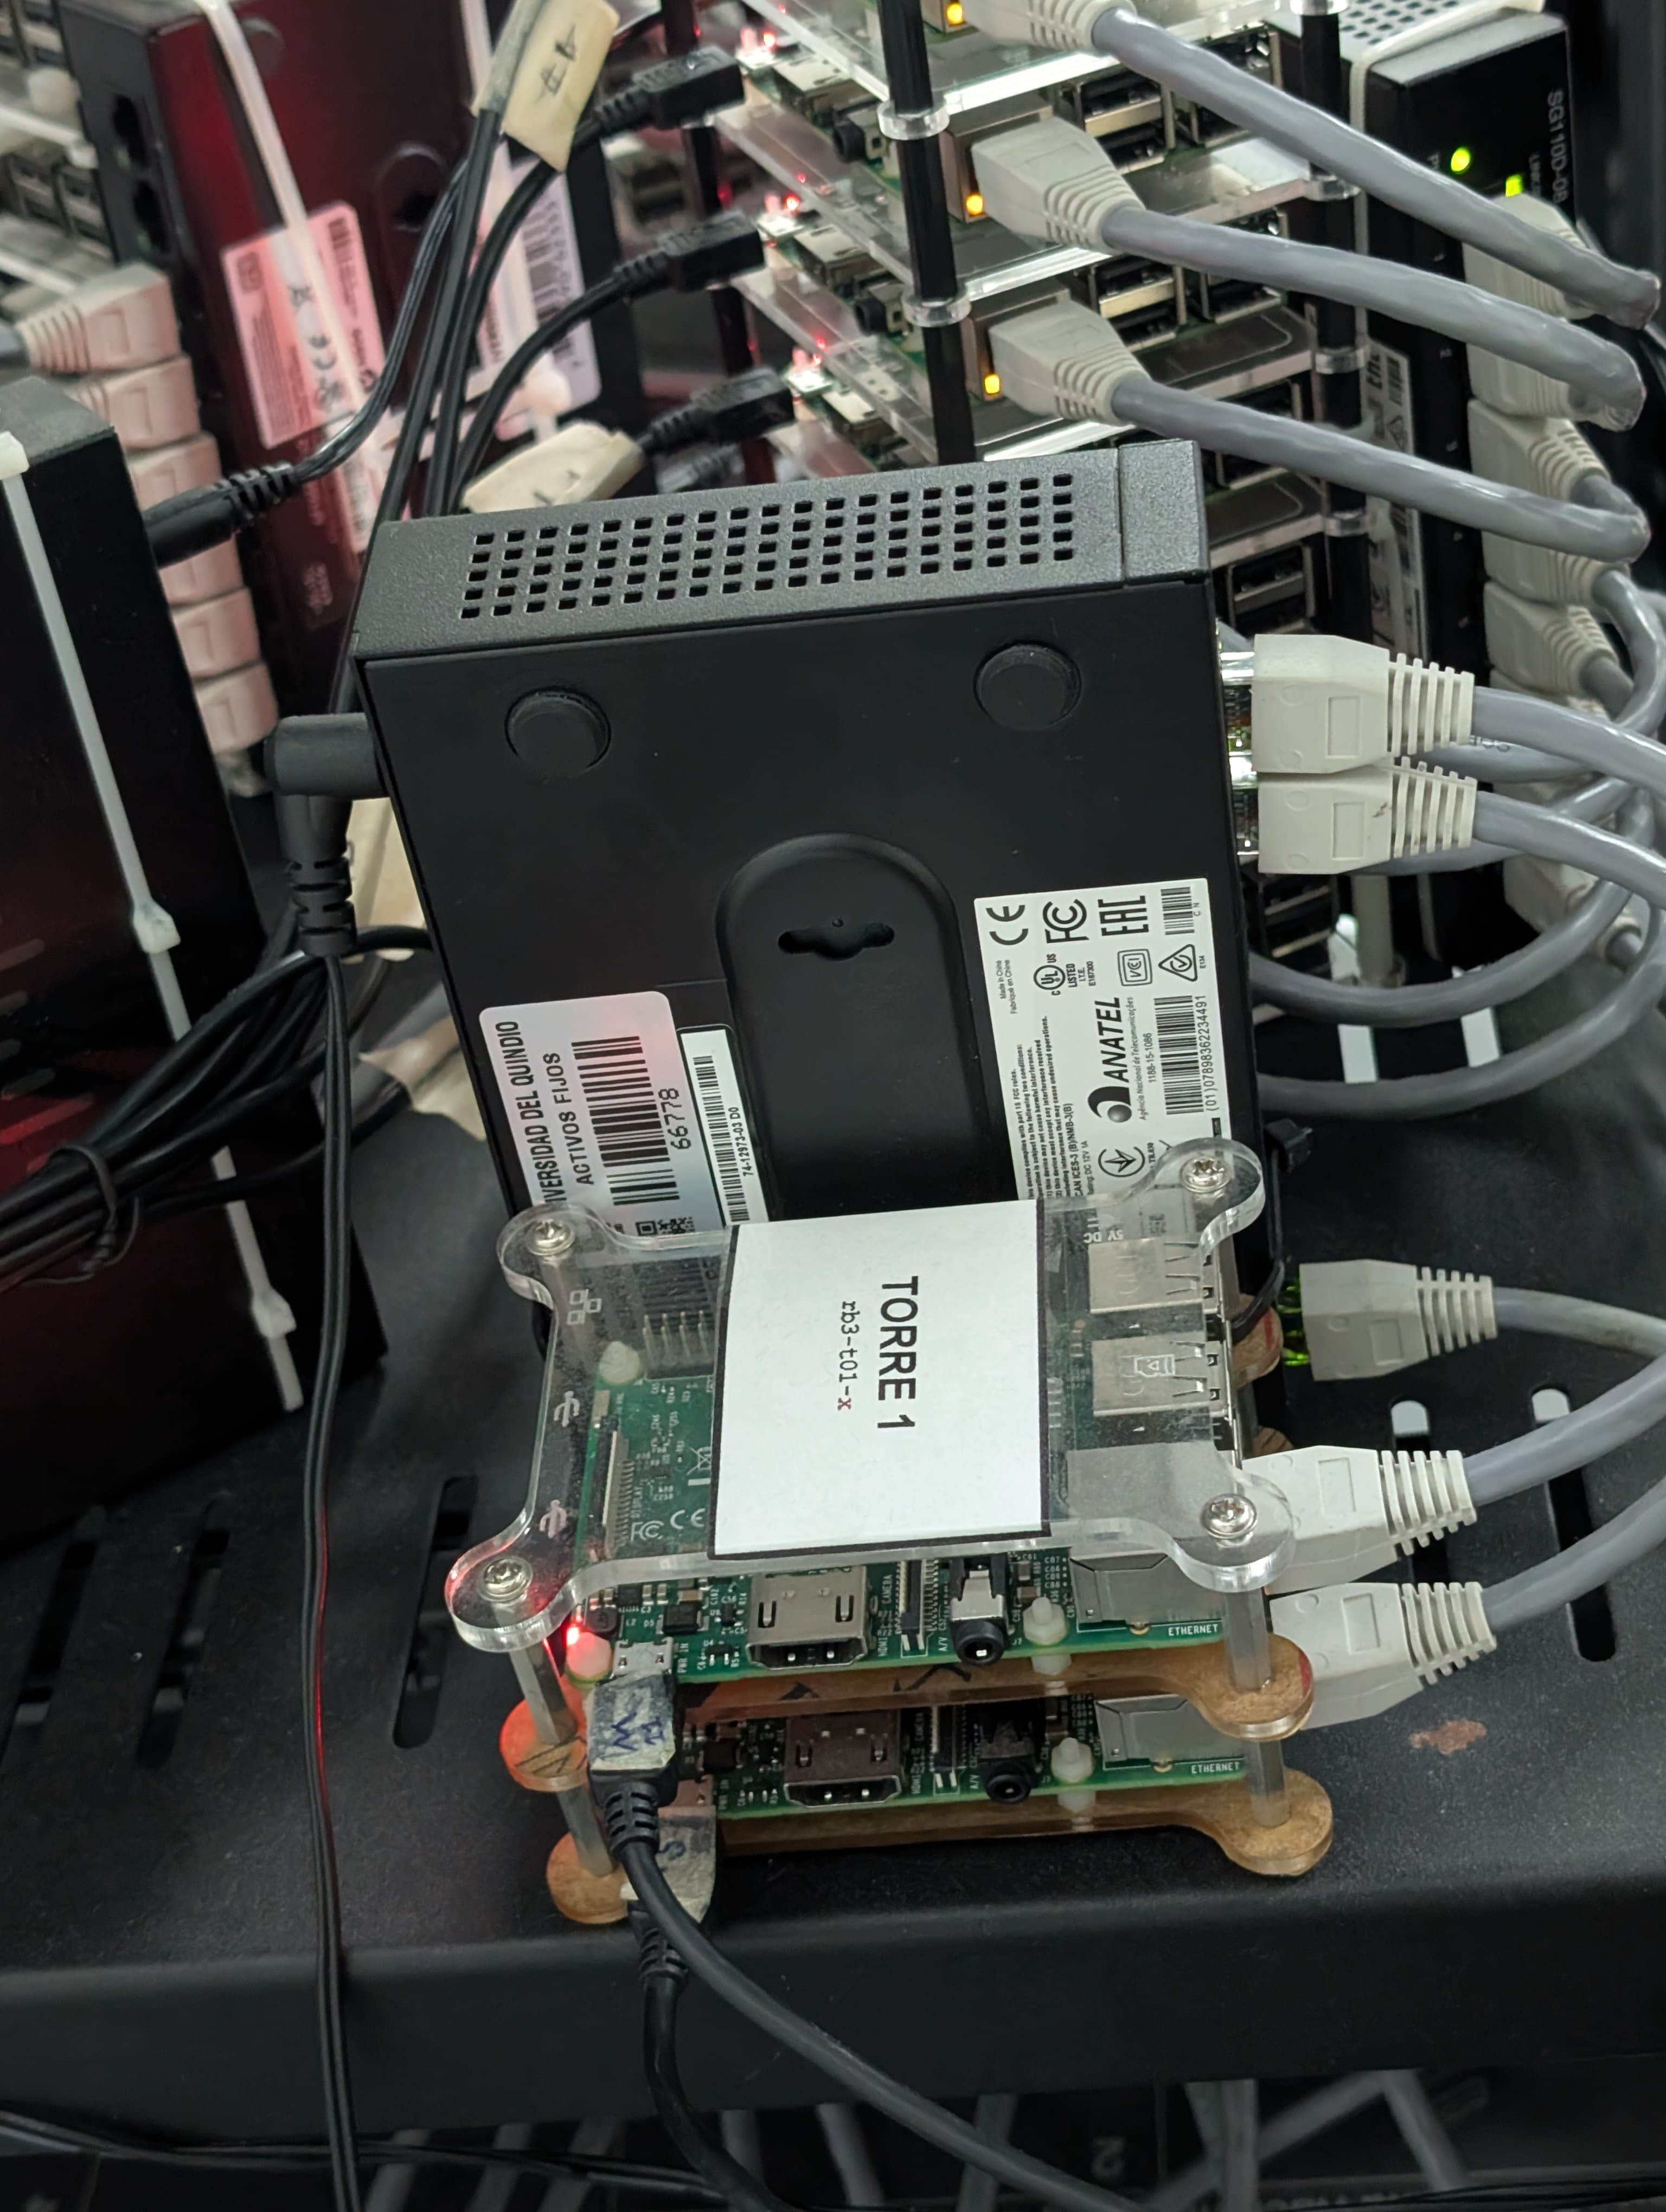
\includegraphics[scale=0.065]{tablas-images/raspberries/torre-binaria.jpeg}
	\caption{Vista general de las máquinas submit y master}
	\label{fig:foto-torre-binaria}
\end{figure}


% ####################################################################################################

\noindent
En la figura \ref{fig:foto-torre-binaria} se muestran las máquinas submit y master de clúster HTCondor.

\noindent
Como se puede evidenciar en las figuras \ref{fig:foto-torres-rasp} y \ref{fig:foto-torre-binaria}, cada máquina perteneciente a una torre está conectada a un switch. Las especificiones de dicho switch se mencionan en la tabla \ref{table:mini-switch}

% filepath: /Users/esteban/git-repos/ht-latex/tablas-images/raspberries/mini-switch.tex
%% Caracteristicas del switch al que están conectadas todas las maquinas HTCondor. 

\begin{table}[H]
	\centering
	\sffamily\scriptsize
	\setlength{\tabcolsep}{4pt}
	\renewcommand{\arraystretch}{1.3}
	\caption{Ficha técnica --- Switch Cisco SF100D-08}\label{table:mini-switch}
	\begin{tabular}{|p{0.25\textwidth}|p{0.6\textwidth}|p{0.12\textwidth}|}
		\hline
		\rowcolor{gray!15} \multicolumn{3}{|c|}{\textbf{DESCRIPCIÓN FÍSICA:} Switch de ocho puertos}                                                                                 \\ \hline

		\textbf{TIPO DE RECURSO:}                    & Switch       & \multirow{3}{*}{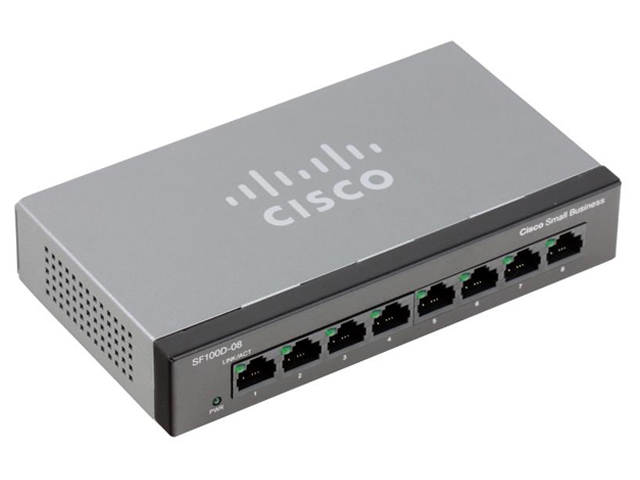
\includegraphics[width=\linewidth,keepaspectratio]{tablas-images/raspberries/mini-switch.jpg}} \\ \cline{1-2}
		\textbf{MODELO:}                             & SF100D-08 V2 &                                                                                                                \\ \cline{1-2}
		\textbf{MARCA:}                              & Cisco        &                                                                                                                \\ \hline

		\rowcolor{gray!15} \multicolumn{3}{|c|}{\textbf{ESPECIFICACIONES TÉCNICAS}}                                                                                                  \\ \hline

		\textbf{Rendimiento}                         &
		\begin{minipage}[t]{\linewidth}
			\vspace{2pt}
			• Capacidad de Conmutación: 1.6 Gbps \\
			• Capacidad de Reenvío: 1.4 mpps \\
			• Prevención de bloqueo HOL \\
			• Jumbo Frames: 9216 bytes
			\vspace{2pt}
		\end{minipage}      &                                                                                                                                         \\ \hline

		\textbf{Interfaces}                          &
		\begin{minipage}[t]{\linewidth}
			\vspace{2pt}
			• 8 puertos RJ-45 10BASE-T/100BASE-TX \\
			• Auto-negociación 10/100 Mbps \\
			• 4 colas de hardware (niveles de prioridad)
			\vspace{2pt}
		\end{minipage} &                                                                                                                                  \\ \hline

		\textbf{Estándares}                          &
		\begin{minipage}[t]{\linewidth}
			\vspace{2pt}
			• 802.3 10BASE-T Ethernet \\
			• 802.3u 100BASE-TX Fast Ethernet \\
			• 802.3x control de flujo \\
			• 802.1p prioridad \\
			• 802.3az Energy Efficient Ethernet
			\vspace{2pt}
		\end{minipage}         &                                                                                                                                           \\ \hline

		\textbf{Características Físicas}             &
		\begin{minipage}[t]{\linewidth}
			\vspace{2pt}
			• Alimentación: DC 12V, 500mA \\
			• Dimensiones: 140 × 33.35 × 140 mm \\
			• Peso: 0.38 kg \\
			• Montaje: Escritorio
			\vspace{2pt}
		\end{minipage}       &                                                                                                                                          \\ \hline

		\textbf{Certificaciones}                     &
		\begin{minipage}[t]{\linewidth}
			\vspace{2pt}
			UL (UL 60950), CSA (CSA 22.2), \\
			CE mark, FCC Part 15 Class A
			\vspace{2pt}
		\end{minipage}            &                                                                                                                                               \\ \hline

		\rowcolor{gray!15} \multicolumn{3}{|l|}{\textbf{PROPÓSITO:} Conexión de red para equipos del cluster HTCondor}                                                               \\ \hline
		\rowcolor{gray!15} \multicolumn{3}{|l|}{\textbf{OPORTUNIDAD DE USO:} Proyectos del \GRID}                                                                                    \\ \hline
		\multicolumn{3}{|p{0.97\textwidth}|}{\textbf{OBSERVACIONES:} Equipo de conectividad que proporciona comunicación entre todos los nodos del cluster HTCondor.}                \\ \hline
	\end{tabular}
\end{table}

\noindent
A su vez, los switch anteriores van conectados a otro switch. Este switch es el Cisco SG200-26. Sus especificaciones pueden verse en la tablas \ref{table:big-switch}

%% Características del switch principal del GRID

\begin{table}[H]
	\centering
	\sffamily\scriptsize
	\setlength{\tabcolsep}{4pt}
	\renewcommand{\arraystretch}{1.3}
	\caption{Ficha técnica --- Switch Cisco SG200-26}
	\label{table:big-switch}
	\begin{tabular}{|p{0.25\textwidth}|p{0.6\textwidth}|p{0.12\textwidth}|}
		\hline
		\rowcolor{gray!15} \multicolumn{3}{|c|}{\textbf{DESCRIPCIÓN FÍSICA:} Switch administrable de 26 puertos}                                                                                                                                 \\ \hline

		\textbf{TIPO DE RECURSO:}                     & Switch Gigabit administrable & \multirow{3}{*}{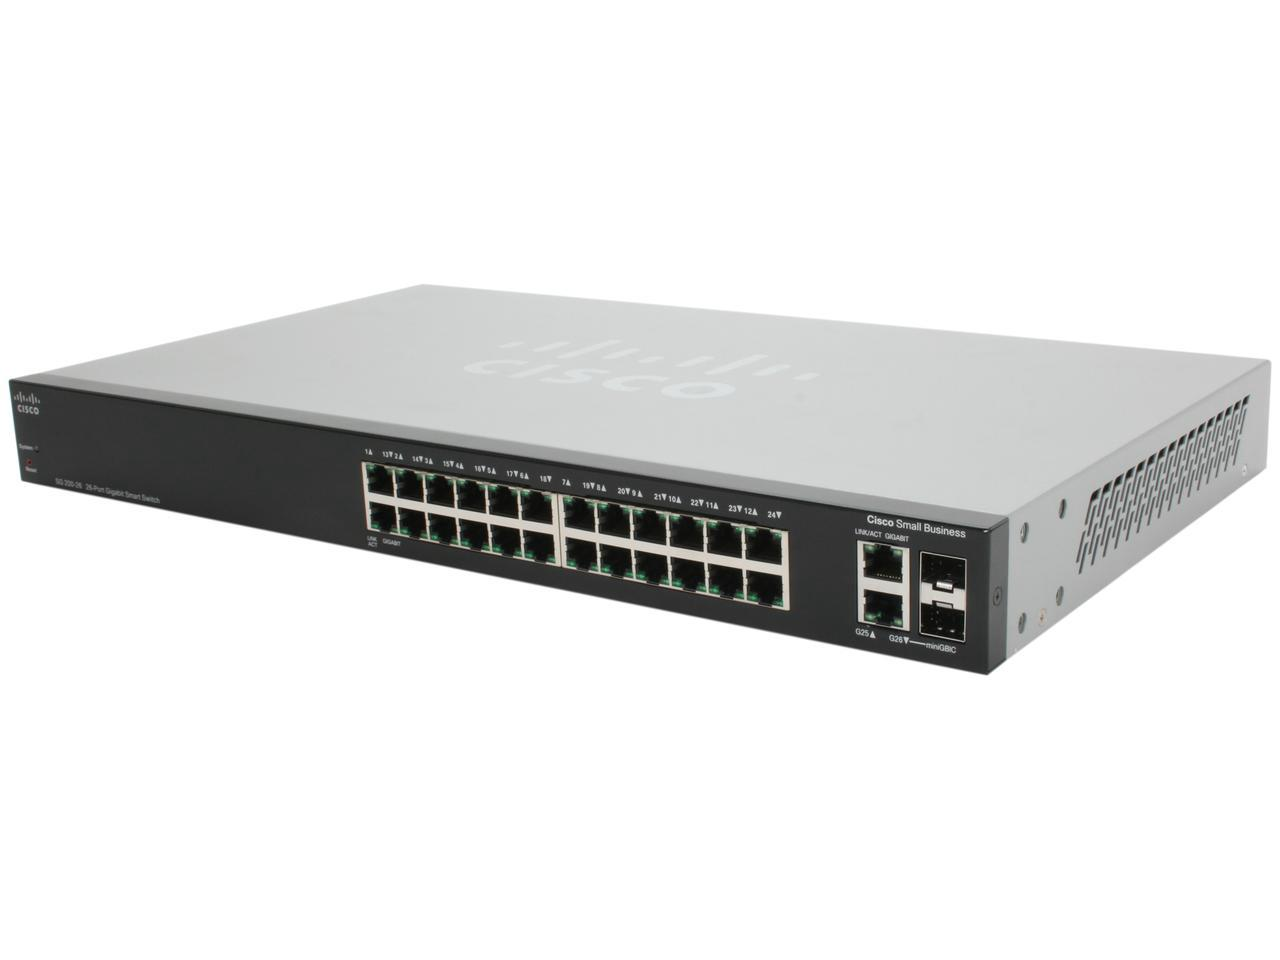
\includegraphics[width=\linewidth,keepaspectratio]{tablas-images/raspberries/big-switch.jpg}}                                             \\ \cline{1-2}
		\textbf{MODELO:}                              & SG200-26                     &                                                                                                                                                           \\ \cline{1-2}
		\textbf{MARCA:}                               & Cisco                        &                                                                                                                                                           \\ \hline

		\rowcolor{gray!15} \multicolumn{3}{|c|}{\textbf{ESPECIFICACIONES TÉCNICAS}}                                                                                                                                                              \\ \hline

		\textbf{Rendimiento}                          &
		\begin{minipage}[t]{\linewidth}
			\vspace{2pt}
			• Capacidad de Conmutación: 52 Gbps \\
			• Capacidad de Reenvío: 38.69 Mpps \\
			• Tabla de direcciones MAC: 8,000 entradas \\
			• Jumbo Frames: Soportado
			\vspace{2pt}
		\end{minipage} &                                                                                                                                                                                               \\ \hline

		\textbf{Interfaces}                           &
		\begin{minipage}[t]{\linewidth}
			\vspace{2pt}
			• 24 puertos RJ-45 10/100/1000 Mbps \\
			• 2 puertos combo Gigabit SFP \\
			• Auto-negociación y auto-MDI/MDIX \\
			• Soporte IEEE 802.3ad (Link Aggregation)
			\vspace{2pt}
		\end{minipage}     &                                                                                                                                                                                                 \\ \hline

		\textbf{Administración}                       &
		\begin{minipage}[t]{\linewidth}
			\vspace{2pt}
			• Interfaz web de administración \\
			• SNMP, RMON, HTTP, TFTP \\
			• Cisco Discovery Protocol \\
			• Auto SmartPorts \\
			• Soporte DHCP y BOOTP
			\vspace{2pt}
		\end{minipage}           &                                                                                                                                                                                                         \\ \hline

		\textbf{Características Avanzadas}            &
		\begin{minipage}[t]{\linewidth}
			\vspace{2pt}
			• VLAN support (IEEE 802.1Q) \\
			• Quality of Service (QoS) \\
			• IGMP/MLD Snooping \\
			• Spanning Tree (STP/RSTP) \\
			• IEEE 802.1x Authentication \\
			• Storm Control (Broadcast/Multicast/Unicast)
			\vspace{2pt}
		\end{minipage} &                                                                                                                                                                                             \\ \hline

		\textbf{Características Físicas}              &
		\begin{minipage}[t]{\linewidth}
			\vspace{2pt}
			• Alimentación: 100-240V AC, 50-60 Hz \\
			• Dimensiones: 439 × 257 × 43 mm \\
			• Peso: 3.3 kg (7.2 lbs) \\
			• Montaje: Rack 1U \\
			• Diseño sin ventiladores
			\vspace{2pt}
		\end{minipage}      &                                                                                                                                                                                                    \\ \hline

		\textbf{Memoria y Estándares}                 &
		\begin{minipage}[t]{\linewidth}
			\vspace{2pt}
			• Flash: 16 MB, RAM: 128 MB \\
			• IEEE 802.3/802.3u/802.3z/802.3ab \\
			• Certificaciones: UL 60950, FCC Part 15A \\
			• MTBF: 194,278 horas
			\vspace{2pt}
		\end{minipage}  &                                                                                                                                                                                                \\ \hline

		\rowcolor{gray!15} \multicolumn{3}{|l|}{\textbf{PROPÓSITO:} Switch principal para interconexión de infraestructura GRID}                                                                                                                 \\ \hline
		\rowcolor{gray!15} \multicolumn{3}{|l|}{\textbf{OPORTUNIDAD DE USO:} Backbone de red para servicios del \GRID}                                                                                                                           \\ \hline
		\multicolumn{3}{|p{0.97\textwidth}|}{\textbf{OBSERVACIONES:} Switch administrable de nivel empresarial que proporciona conectividad Gigabit con funciones avanzadas de gestión, VLAN, QoS y seguridad para la infraestructura del GRID.} \\ \hline
	\end{tabular}
\end{table}


\subsection{Ambientes de ejecución de la infraestructura HTCondor del \GRID}
\noindent{}
De acuerdo con la documentación oficial de HTCondor \citep{HTCondor-choosing-universe}, un universo se define como el ambiente de ejecución en el cual se lleva a cabo un trabajo. Al momento del desarrollo de la presente investigación, HTCondor contempla nueve universos disponibles: \textit{vanilla, grid, java, scheduler, local, parallel, vm, container} y \textit{docker}. Cada trabajo demanda, en función de sus características particulares, condiciones específicas de ejecución. A modo de ejemplo, un trabajo constituido por un programa desarrollado en lenguaje Java puede obtener ventajas significativas mediante la utilización del universo Java, lo cual facilita al usuario la configuración del ambiente de ejecución requerido.

Hasta el momento, la configuración de HTCondor del \GRID únicamente incorpora el universo vanilla, el cual está orientado a la ejecución no especializada de programas. En otras palabras, se trata de un universo de propósito general en el que los scripts de Shell han demostrado ser particularmente efectivos \citep{HTCondor-choosing-universe}.


\subsection{Servicios actuales de computación distribuida}
\noindent
Los servicios actuales del \GRID se orientan principalmente hacia la provisión de infraestructura de \TI, abarcando máquinas virtuales, soluciones de almacenamiento y configuración de redes. No obstante, la computación distribuida constituye un dominio especializado que demanda competencias técnicas avanzadas por parte de los usuarios. En consecuencia, si bien el grupo ha desarrollado capacidades en esta área, aún no se ha consolidado una oferta formal de servicios de computación distribuida de acceso público para la comunidad académica institucional.

% !TODO PREGUNTA PARA EL PROFE: Aquí hago una declaración temeraria sobre la universidad que neceisto confirmar
% Se han ofrecido servicios de computación identifica en el grupo grid que hayan estado disponibles para otros grupos o para 
% los mismo estudiantes de la universidad? 
%
\subsection{Servicios de computación distribuida esperados}
\noindent
Dado que no se ha establecido previamente un servicio de computación distribuida basado en HTCondor con acceso abierto para la comunidad educativa, resulta necesario identificar los potenciales beneficiarios que podrían aprovechar esta tecnología. Como señalan \cite{Wilson2016}, la computación se ha consolidado como un componente crítico del proceso científico en prácticamente todas las disciplinas, independientemente de su orientación hacia la experimentación o la simulación computacional. En este contexto, los usuarios que obtendrían mayor beneficio de la implementación de un servicio de computación distribuida serían aquellos cuyas actividades académicas o investigativas demanden capacidades de procesamiento intensivo para la obtención de resultados científicos. Por consiguiente, se estima que los principales beneficiarios de esta infraestructura serían tanto los estudiantes, quienes podrían fortalecer significativamente su proceso formativo mediante el acceso a una ambiente de computación distribuida, como los grupos de investigación institucionales, que verían ampliadas sus capacidades para desarrollar proyectos de mayor envergadura computacional. En la tabla \ref{table:servicio-htcondor} se especifica cómo podría verse un servicio de computación de alta productividad basado en HTCondor.

\begin{table}[H]
	\centering
	\sffamily\scriptsize
	\setlength{\tabcolsep}{4pt}
	\renewcommand{\arraystretch}{1.3}
	\caption{Caracterización del servicio de computación distribuida HTCondor esperado para el GRID}
	\label{table:servicio-htcondor}
	\begin{tabular}{|p{0.28\textwidth}|p{0.67\textwidth}|}
		\hline
		\rowcolor{gray!15} \multicolumn{2}{|c|}{\textbf{DESCRIPCIÓN GENERAL DEL SERVICIO}}                                                                                                                                                                                            \\ \hline

		\textbf{NOMBRE DEL SERVICIO}       & Servicio de Computación Distribuida HTCondor                                                                                                                                                                                             \\ \hline
		\textbf{TIPO DE SERVICIO}          & Servicio de educación, investigación y extensión universitaria                                                                                                                                                                           \\ \hline
		\textbf{HORARIO DE DISPONIBILIDAD} & 24/7 (Disponibilidad continua)                                                                                                                                                                                                           \\ \hline

		\rowcolor{gray!15} \multicolumn{2}{|c|}{\textbf{OBJETIVOS Y ALCANCE}}                                                                                                                                                                                                         \\ \hline

		\textbf{PROPÓSITO}                 &
		\begin{minipage}[t]{\linewidth}
			\vspace{2pt}
			Proveer infraestructura de computación de alta productividad (\HTC) para la ejecución de tareas computacionales intensivas y paralelas, facilitando el procesamiento distribuido de cargas de trabajo científicas y académicas
			\vspace{2pt}
		\end{minipage}                                                 \\ \hline

		\textbf{USUARIOS OBJETIVO}         &
		\begin{minipage}[t]{\linewidth}
			\vspace{2pt}
			• Estudiantes de pregrado y posgrado \\
			• Grupos de investigación institucionales \\
			• Docentes investigadores \\
			• Comunidad académica UQ
			\vspace{2pt}
		\end{minipage}                                                                                                                                                                                                                                     \\ \hline

		\rowcolor{gray!15} \multicolumn{2}{|c|}{\textbf{ESPECIFICACIONES TÉCNICAS}}                                                                                                                                                                                                   \\ \hline

		\textbf{RECURSOS DE HARDWARE}      &
		\begin{minipage}[t]{\linewidth}
			\vspace{2pt}
			• Clúster de máquinas Raspberry Pi \\
			• Máquinas virtuales especializadas \\
			• Infraestructura de red dedicada
			\vspace{2pt}
		\end{minipage}                                                                                                                                                                                                                                           \\ \hline

		\textbf{TECNOLOGÍAS}               &
		\begin{minipage}[t]{\linewidth}
			\vspace{2pt}
			• HTCondor (High Throughput Computing) \\
			• Sistemas de virtualización \\
			\vspace{2pt}
		\end{minipage}                                                                                                                                                                                                                                        \\ \hline

		\textbf{CAPACIDADES}               &
		\begin{minipage}[t]{\linewidth}
			\vspace{2pt}
			• Procesamiento paralelo de tareas independientes \\
			• Gestión automática de recursos \\
			• Balanceo de carga dinámico \\
			• Tolerancia a fallos
			\vspace{2pt}
		\end{minipage}                                                                                                                                                                                                                             \\ \hline

		\rowcolor{gray!15} \multicolumn{2}{|c|}{\textbf{APLICACIONES Y BENEFICIOS}}                                                                                                                                                                                                   \\ \hline

		\textbf{CASOS DE USO}              &
		\begin{minipage}[t]{\linewidth}
			\vspace{2pt}
			• Simulaciones científicas y modelado matemático \\
			• Procesamiento de datos masivos (Big Data) \\
			• Renderización de video y gráficos \\
			• Análisis bioinformático y genómico \\
			\vspace{2pt}
		\end{minipage}                                                                                                                                                                                                                              \\ \hline

		\textbf{IMPACTO ESPERADO}          &
		\begin{minipage}[t]{\linewidth}
			\vspace{2pt}
			• Fortalecimiento de capacidades investigativas \\
			• Democratización del acceso a recursos HTC \\
			• Apoyo a formación en computación distribuida \\
			• Incremento en productividad científica \\
			• Posicionamiento institucional en \HTC
			\vspace{2pt}
		\end{minipage}                                                                                                                                                                                                                               \\ \hline

		\rowcolor{gray!15} \multicolumn{2}{|l|}{\textbf{CONTRIBUCIÓN:} Expansión de universos HTCondor para mayor versatilidad}                                                                                                                                                       \\ \hline
		\multicolumn{2}{|p{0.95\textwidth}|}{\textbf{OBSERVACIONES:} Servicio orientado a democratizar el acceso a recursos de computación de alto rendimiento para la comunidad académica, fortaleciendo las capacidades investigativas y formativas de la Universidad del Quindío.} \\ \hline
	\end{tabular}
\end{table}
\section{Descripción de la oportunidad}
\noindent
La implementación de un nuevo universo HTCondor en la infraestructura del grupo GRID representa una oportunidad estratégica de considerable valor tanto para la comunidad académica de la Universidad del Quindío como para los grupos de investigación locales y externos. En primer lugar, esta ampliación abrirá el paso para que diversos grupos de investigación de la institución accedan a capacidades computacionales especializadas más diversas, democratizando así el uso de tecnologías de computación distribuida para disciplinas que requieren procesamiento intensivo de datos, tales como la bioinformática, el análisis de big data, el aprendizaje profundo y la simulación científica. En segundo lugar, desde una perspectiva formativa, la incorporación de este nuevo universo constituye una oportunidad invaluable para que los estudiantes de pregrado y posgrado adquieran competencias prácticas en computación de alto rendimiento (\HTC), un campo con limitada documentación y experiencias de implementación documentadas en el contexto colombiano. Adicionalmente, esta iniciativa ayudaría al posicionamiento del \GRID como un referente en computación distribuida a nivel nacional, facilitando la colaboración interinstitucional y el desarrollo de proyectos conjuntos con otras universidades e instituciones de investigación. Finalmente, la consolidación de una infraestructura HTCondor más robusta y versátil contribuye directamente a la competitividad investigativa de la Universidad del Quindío, optimizando el aprovechamiento de recursos computacionales disponibles y generando capacidades técnicas diferenciadas que pueden traducirse en publicaciones científicas, proyectos de mayor envergadura y fortalecimiento de las líneas de investigación institucionales.


\section{Resumen de la entrevista con el cliente}

Para comprender mejor las necesidades y expectativas del \GRID\, se realizó una entrevista con el cliente.

%!TODO  Entrevista
\begin{itemize}
	\item \textbf{Entrevistado:} Luis Eduardo Sepúlveda Rodríguez
	\item \textbf{Fecha:} XXXXXXXXX
	\item \textbf{Duración:} XXXXXXXXXXX
	\item \textbf{Link:} \href{https://drive.google.com}{click aquí}
	\item \textbf{Asistentes:} Juan Esteban Castaño Osma, Juan Esteban Parra Parra
\end{itemize}

\ChapterImageStar[cap:caracterizacion-universos]{Caracterización de los Universos HTCondor}{./images/fondo.png}\label{cap:caracterizacion-universos}
\mbox{}\\

En esta sección se presenta una descripción detallada de los distintos universos que conforman HTCondor. Cada universo representa un entorno de ejecución específico, diseñado para satisfacer diferentes necesidades computacionales y facilitar la integración de diversas aplicaciones científicas y técnicas. Se analizan sus principales características, ventajas y limitaciones, proporcionando una visión integral que permita seleccionar el universo más adecuado según los requerimientos de cada proyecto.



\section{Universos disponibles}

Como se ha mencionado anteriormente, HTCondor es un sofisticado sistema de software diseñado para la \textbf{Computación de Alto Rendimiento} (\HTC) que gestiona vastos recursos computacionales al emparejar a los propietarios de recursos con los consumidores de recursos \citep{HTCondor}. Un concepto fundamental dentro de este software es el de los \textit{Universos}, los cuales definen el entorno de ejecución específico, las reglas de gestión de recursos y la semántica de fallos.

La selección del universo se define en el archivo de descripción de envío (también conocido como \textit{submit file}) y determina principalmente la forma en que el trabajo interactúa con el pool de recursos computacionales. Esta elección especifica aspectos como por ejemplo si la ejecución será local o remota, tal y como ocurre en el universo \textit{Grid}, o si se debe buscar algún binario específico para la ejecución, como en el caso del universo \textit{java}. Hasta la fecha de redacción de este documento, los principales universos soportados son los siguientes \citep{HTCondor-choosing-universe}:

\begin{itemize}
	\item \textbf{\textit{Vanilla}}
	\item \textbf{Grid}
	\item \textbf{Java}
	\item \textbf{\textit{Scheduler}}
	\item \textbf{Local}
	\item \textbf{Parallel}
	\item \textbf{VM}
	\item \textbf{Container}
	\item \textbf{Docker}
\end{itemize}

\subsection{\textit{Vanilla}}

El universo \textit{Vanilla} sirve como el entorno de ejecución \textbf{predeterminado} y más ampliamente utilizado en HTCondor. Está destinado específicamente a la gran mayoría de los programas de usuario, ofreciendo las menores restricciones y el más alto nivel de compatibilidad general. Si un administrador o usuario no especifica explícitamente un universo en el archivo \textit{submit}, se asume automáticamente que el universo escogido es el \textit{Vanilla} \citep{CERNBatchDocs}.



La flexibilidad inherente del universo \textit{Vanilla} significa que, para cargas de trabajo nuevas o especializadas, los administradores y desarrolladores frecuentemente priorizan adaptarlas para que se ejecuten dentro de este entorno. Por ejemplo, algunos trabajos requieren de envolver aplicaciones paralelas o pilas de dependencias complejas dentro de contenedores (\textit{Docker o Singularity}) y lanzarlas como un simple \textit{wrapper} ejecutable bajo el universo \textit{Vanilla}, estableciendo efectivamente el universo \textit{Vanilla} como la capa de compatibilidad universal para los flujos de trabajo modernos de alto rendimiento \citep{Emilio_DockerHTCondor, HTCondor_Parallel}.


\subsection{Local}

El universo \textit{Local} es aquel con el cual es posible ejecutar trabajos en la máquina \textit{submit}.

Los trabajos en el universo local presentan las siguientes características \citep{HTCondor-choosing-universe}:

\begin{itemize}
	\item Se ejecutan \textbf{inmediatamente} tras el envío
	\item No entran en el ciclo de negociación
	\item Omiten el proceso típico de emparejamiento
\end{itemize}


\subsection{\textit{Scheduler}}

Según la documentación oficial de \cite{HTCondor-choosing-universe}, el universo \textit{Scheduler} es esencialmente el mismo que el universo \textit{Local}, sin embargo, a diferencia de este último, el universo \textit{Scheduler} no utiliza un demonio \texttt{condor\_starter} para gestionar el trabajo y por lo tanto, ofrece funciones y soporte de políticas limitados.

\section{Universos con entornos de ejecución especializados}

Estos universos están diseñados para cargas de trabajo que requieren entornos de tiempo de ejecución de programación específicos o esquemas complejos de asignación de recursos que involucran múltiples máquinas concurrentes.

\subsection{Universo Java}

El universo Java está ajustado para trabajos escritos en este lenguaje, diseñados para ejecutarse en la Máquina Virtual de Java (JVM). Aunque es posible ejecutar aplicaciones Java en el universo \textit{Vanilla}, el universo Java incluye características especializadas que simplifican y facilitan su ejecución. Por ejemplo, como señalan \cite{Thain2002}, anteriormente los usuarios debían enviar el binario de la JVM bajo el universo \textit{standard} (un universo antiguo de HTCondor que ha sido reemplazado por el universo \textit{Vanilla}) para ejecutar programas Java. Actualmente, basta con enviar el archivo \texttt{.class} en el archivo \textit{submit}, permitiendo que el trabajo se ejecute directamente en los nodos ejecutores que cumplen con los requisitos necesarios para ejecutar un trabajo Java.

\subsection{Parallel}

El universo \textit{Parallel} está diseñado para dar soporte a trabajos que requieren ejecución síncrona en múltiples máquinas de ejecución dedicadas. Es esencial para aplicaciones estrechamente acopladas, más comúnmente aquellas que utilizan el paradigma \textbf{\textit{Message Passing Interface} (MPI)}, y reemplaza al universo \textbf{mpi} más antiguo \citep{HTCondor-env-services}.


Según la documentación oficial de \citep{HTCondor-env-services} en el universo \textit{Parallel}:

\begin{itemize}
	\item El envío del trabajo especifica el número total de \textit{slots} (o nodos ejecutores) requeridos usando \texttt{machine\_count}
	\item El demonio negociador de HTCondor asegura que todos los recursos necesarios se reclamen \textbf{concurrentemente} antes de que la ejecución pueda comenzar.
	\item HTCondor designa uno de los nodos como ``\textbf{nodo 0}'', que típicamente ejecuta el proceso maestro.
\end{itemize}

HTCondor gestiona la configuración de la comunicación, incluida la generación y copia de claves SSH a través de los nodos asignados para permitir la comunicación sin contraseña necesaria para iniciar la aplicación paralela. También requiere una configuración específica del comportamiento de terminación del trabajo a través de atributos como \texttt{+ParallelShutdownPolicy}~\citep{HTCondor-env-services}.




\section{Entornos de Alto Aislamiento: Contenedores y Máquinas Virtuales}

La necesidad de entornos de ejecución que encapsulen las dependencias de la aplicación, aseguren la reproducibilidad y proporcionen distintos niveles de aislamiento de seguridad ha llevado al desarrollo de universos dedicados para contenedores y virtualización.

\subsection{Docker}

El universo \textit{Docker} permite que un trabajo HTCondor se ejecute directamente dentro de un contenedor Docker. Este universo proporciona aislamiento de procesos a nivel de sistema operativo, utilizando la funcionalidad estándar de Docker para ejecutar imágenes definidas por el usuario.

\subsubsection{Requisitos e Integración}

La ejecución en el universo \textit{Docker} requiere:

\begin{itemize}
	\item El servicio Docker debe estar preinstalado y configurado en los nodos ejecutores.
	\item El envío del trabajo debe especificar el nombre de la imagen del contenedor usando \texttt{docker\_image}.
\end{itemize}


\subsection{Container}

El universo \textit{Container} ofrece un enfoque más flexible que el universo Docker, abstrayendo la tecnología de contenerización subyacente para dar soporte a sistemas como Singularity (ahora Apptainer). Esencialmente, lo que el universo \textit{Container} procura es ofrecer una sintaxis que no dé privilegio a un \textit{runtime} específico (como sí ocurre en el universo \textit{Docker}), de manera que cualquier máquina con un \textit{runtime} compatible con la imagen especificada por el usuario pueda ser usada \citep{HTCondor-env-services}.


\subsection{VM}

El universo \textit{VM} facilita la ejecución de una imagen de disco de máquina virtual como un trabajo HTCondor.
\subsubsection{Mecanismo e Integración con el Hipervisor}

En este universo:

\begin{itemize}
	\item El trabajo ya no es un simple ejecutable, sino una \textbf{imagen de disco completa}
	\item HTCondor soporta la integración con hipervisores como Xen, KVM y VMware \citep{HTCondor_vm_universe_wiki}
\end{itemize}

\section{Universos Distribuidos y Federados}

Estos universos abordan la necesidad de integrar y gestionar recursos computacionales que residen fuera de los límites inmediatos del clúster HTCondor, soportando la federación de recursos externos  \citep{Padmanabhan2011}.

\subsection{Grid}

El universo \textit{Grid} permite a los usuarios de HTCondor enviar trabajos a sistemas de gestión remotos, actuando como un puente hacia sistemas de lotes externos como Slurm, LSF u otros \textit{pools} de HTCondor a través del demonio \texttt{condor\_gridmanager}. La gestión de trabajos se realiza mediante protocolos de comunicación especializados \citep{HTCondor-Grid-universe}, lo que permite a las organizaciones utilizar recursos distribuidos a través de dominios administrativos dispares. Esta capacidad facilita colaboraciones científicas a gran escala y la federación de clústeres universitarios o nacionales \citep{Padmanabhan2011}.

%\ChapterImageStar[cap:dar]{Análisis de Decisiones y Resolución}{./images/fondo.png}\label{cap:dar}
\mbox{}\\


\section{Metodología de evaluación}

La metodología de evaluación aplicada para la elección de la tecnología del nuevo universo HTCondor fue \textit{Decision Analysis and Resolution} (\DAR) de \CMMI \citep{CMMIInstitute2010}. Esta metodología permitió evaluar las necesidades del grupo \GRID\ mediante un proceso estructurado que consideró múltiples alternativas, criterios de evaluación bien definidos y un análisis comparativo riguroso. Los criterios evaluados incluyeron el nivel de acoplamiento de trabajos (entendido como la capacidad de un universo para sincronizar múltiples trabajos entre sí), la capacidad de interrupción de trabajos como mecanismo para mejorar la calidad de servicio, la popularidad y adopción en el contexto académico, y la disponibilidad y calidad de documentación técnica del universo. El uso de \DAR\ no solo aporta transparencia y trazabilidad al proceso de selección, sino que también garantiza objetividad y justificación técnica sólida para la decisión arquitectónica de incorporar un nuevo universo HTCondor.

\subsection{Lista de criterios}
A continuación se describen los criterios seleccionados para la evaluación.

\subsubsection{Capacidad de paralelismo puro}
\textbf{Código:} PARALLEL

\textbf{Descripción:} Este criterio evalúa la capacidad de los diferentes universos para ejecutar computación paralela pura por medio de la comunicación entre procesos a través de algún mecanismo de \MPI como OpenMPI.

\textbf{Justificación:} En el contexto de la Universidad del Quindío es deseable para el
grupo \GRID desarrollar capacidades paralelas puras en su clúster de HTCondor por
diferentes razones tales como la ejecución sincronizada y simultánea de trabajos o
la comunicación entre procesos, algunos usos de estas capacidades paralelas
pueden ser la ejecución de simulaciones distribuidas en las que la sincronización de
los trabajos es crítica debido a la ganancia temporal fruto de la comunicación en
tiempo real de los procesos, el entrenamiento paralelo de redes neuronales en el
que los pesos se actualizan de forma dinámica con la información enviada por cada
proceso paralelo, entro otros. Los casos descritos anteriormente son algunos de los
muchos en los que el soporte para trabajos paralelos puede ser deseable para el
grupo de investigación \GRID, por lo que su inclusión como criterio en la toma de
decisión se considera adecuada, no como una necesidad infalible sino como un
valor adicional. Si esta fuese una necesidad infalible, entonces aquellos Universos
que no cumpliesen con capacidad para paralelismo quedarían descartados
automáticamente.

\subsubsection{Soporte para checkpointing}
\textbf{Código:} CHECKPOINTING

\textbf{Descripción:}Este criterio se refiere a la capacidad de un Universo para soportar o
no el \textit{checkpointing}. Con este término nos referimos a la capacidad de un trabajo
para ser retomado o reanudado después de su interrupción, persistiendo los valores
calculados por el proceso interrumpido hasta ese momento. Este criterio se
considera binario, ya que un Universo puede tener o no esta capacidad, cabe aclarar
que HTCondor define ciertos mecanismos de \textit{checkpointing} en su documentación
mas no aclara muy bien en cuáles Universos pueden o no ser usados, sin embargo,
es posible programar estas capacidades en capa de aplicación, lo cual se toma en
cuenta para este criterio. El único caso especial es aquel del Universo Parallel, en
el cual, según se explica en la documentación encontrada, no es posible
implementar \textit{checkpointing} debido a la naturaleza de ejecución de sus trabajos. En
los demás universos los trabajos se ejecutan de manera atómica (excepto
posiblemente el Universo Grid), es decir, de manera independiente en cada nodo,
sin embargo, la capa adicional que ofrece el \MPI en el Universo Parallel hace que
el estado actual de un trabajo no se encuentre en uno solo, sino que se encuentre
simultáneamente en todos los nodos, así como también en aquellos mensajes que
aún se encuentren en la red.


\textbf{Justificación:} La continuidad de servicio es una característica deseable para la
mayoría de las organizaciones de la industria 4.0 y el grupo \GRID no es la
excepción. En este tipo de computación un nodo podría eventualmente presentar
indisponibilidad a mitad de la ejecución de un trabajo HTCondor, en este sentido el
\textit{checkpointing} se presenta como un mecanismo para evitar la pérdida de trabajo en
caso de que esto ocurra. Así pues, la capacidad para \textit{checkpointing} se considera
importante para que el grupo \GRID pueda llegar a ofrecer servicios de computación
tolerantes a la variación en el estrés computacional de su infraestructura distribuida
a través de HTCondor.



\subsubsection{Popularidad}
\textbf{Código:} POPULARITY

\textbf{Descripción:} Se refiere a la cantidad de artículos, fruto del mapeo sistemático
hecho con antelación, que mencionan o indican de una u otra forma el uso o
preferencia hacia el uso de un Universo, para el problema que se aborda en los
casos de estudio propuestos por dichos artículos, para la extracción de este
criterio se realizó un proceso riguroso de estudio de mapeo sistemático en el que
se analizó parte de la literatura y se encontró la tendencia de uso de cada
Universo, al ser una medida numérica se dividió en 3 cuantiles (intervalos) de igual
tamaño y se calificó con base en qué intervalo se ubicaba cada número.


\textbf{Justificación:}Las tendencias en el uso de cada Universo en el ámbito académico
es un indicador importante de la utilidad y uso de cada Universo en ciertos casos
de estudio, a pesar de no replicar exactamente el Universo de un caso de estudio
similar, se toman casos de estudios que giran en torno a los Universos de
HTCondor, así se extraen métricas que permiten determinarlos Universos más
usados en la literatura consultada.


\subsubsection{Cantidad de documentación académica}
\textbf{Código:} DOC

\textbf{Descripción:} Se refiere a la documentación académica encontrada en torno a
este Universo, específicamente en el motor de búsqueda “Google Scholar”. Este
criterio difiere de la popularidad, ya que se usa un método menos exhaustivo para
su medición, además, en el criterio popularidad solo se toman en cuenta los casos
de estudio en bases de datos específicas, por el contrario, en este caso se hace
una medición general en un motor de búsqueda ampliamente usado. Esta medida
toma relevancia cuando se considera el hecho de que pueden haber Universos
muy populares pero poco documentados, y en tal caso, dichos universos podrían
no ser idóneos para la implementación en la infraestructura HTCondor del \GRID.


\textbf{Justificación:} La cantidad de documentación disponible respecto a cierto
Universo hace más sencilla la correcta documentación de la arquitectura
propuesta para la infraestructura del \GRID, esto cobra relevancia cuando
consideramos que la poca documentación es uno de los problemas hallados en
el diagrama de Ishikawa realizado en torno a las debilidades y problemáticas que
existen alrededor de la infraestructura HTCondor de \GRID y debe ser mitigado
para que ayude a la mitigación del efecto general.

El proceso de categorización de popularidad consistió en realizar búsquedas sistemáticas en Google Scholar para cada universo evaluado, utilizando este motor de búsqueda académico para obtener métricas cuantitativas sobre la frecuencia de aparición en la literatura científica disponible. Los resultados obtenidos se categorizaron en tres cuantiles establecidos en función del universo con mayor número de apariciones, tal como se detalla en la tabla~\ref{tab:popularidad_universos}.


% TABLA Popularidad según Google Scholar.
\begin{table}[H]
	\centering
	\renewcommand{\arraystretch}{1.4} % Espaciado reducido
	\fontsize{9pt}{8pt}\selectfont % Tamaño de fuente 9pt
	\caption{Resultados de búsqueda de popularidad por universo.}
	\label{tab:popularidad_universos}
	\begin{tabular}{|>{\centering\arraybackslash}p{2.0cm}|>{\centering\arraybackslash}p{6.5cm}|>{\centering\arraybackslash}p{2.5cm}|>{\centering\arraybackslash}p{2.0cm}|}
		\hline
		{\textbf{Universo}} & {\textbf{Cadena de búsqueda}}                           & {\textbf{Cantidad de resultados}} & {\textbf{Cuantil [1..3]}} \\
		\hline
		Container           & (``htcondor'' OR ``condor'') AND ``container universe'' & 0                                 & 1                         \\
		\hline
		Docker              & (``htcondor'' OR ``condor'') AND ``docker universe''    & 14                                & 1                         \\
		\hline
		VM                  & (``htcondor'' OR ``condor'') AND ``vm universe''        & 33                                & 1                         \\
		\hline
		Scheduler           & (``htcondor'' OR ``condor'') AND ``scheduler universe'' & 34                                & 1                         \\
		\hline
		Grid                & (``htcondor'' OR ``condor'') AND ``grid universe''      & 60                                & 2                         \\
		\hline
		Local               & (``htcondor'' OR ``condor'') AND ``local universe''     & 74                                & 2                         \\
		\hline
		Java                & (``htcondor'' OR ``condor'') AND ``java universe''      & 79                                & 2                         \\
		\hline
		Vanilla             & (``htcondor'' OR ``condor'') AND ``vanilla universe''   & 163                               & 3                         \\
		\hline
		Parallel            & (``htcondor'' OR ``condor'') AND ``parallel universe''  & 177                               & 3                         \\
		\hline
	\end{tabular}
	\vspace{5pt}
\end{table}


\subsubsection{División de roles}
\textbf{Código:} ROLE DIV

\textbf{Descripción:} Este criterio toma en cuenta la división de roles por máquina.
Esencialmente, los clústeres HTCondor convencionales tienen tres roles: Central
Manager, Submit Node y Execute. En un entorno ideal estos roles deben estar
separados en diferentes máquinas, sin embargo, existen Universos en los que
estos roles no se dividen en varias máquinas y son ejecutados por un solo nodo
de cómputo, lo que no se alinea con las causas que se quieren mitigar.

\textbf{Justificación:} La división de trabajos es una situación deseable para la
infraestructura HTCondor del \GRID, ya que así cada nodo de cómputo tendrá una
única responsabilidad y se evitará sobrecargar un equipo con múltiples funciones
lo que propende por una administración atómica al mismo tiempo que aumenta la
facilidad e implementación mecanismos de recuperación y redundancia a cada
rol.



\subsection{Lista de Universos de HTCondor}
Tras definir los criterios, se identificaron los Universos disponibles en la tecnología HTCondor \citep{HTCondor-choosing-universe}:
\begin{itemize}
	\item vanilla
	\item grid
	\item java
	\item scheduler
	\item local
	\item parallel
	\item vm
	\item container
	\item docker
\end{itemize}

\subsection{Medición de la popularidad}
El criterio de ``popularidad'' se definió como el volumen de uso de un Universo en artículos científicos, por lo que se requirió un proceso metódico para su medición. Para ello, se procedió con un estudio de mapeo sistemático \SMS (ver sección \ref{cap:revisionLiteratura}). El SMS es un método definido para analizar literatura existente, extrayendo recursos de varias fuentes y seleccionándolos con criterios rigurosos. El resultado final es una taxonomía que permite contar las apariciones de cada Universo en la literatura seleccionada.

El proceso completo es robusto e incluye múltiples etapas; sin embargo, para fines de este documento, lo más relevante es el diagrama del proceso (Figura \ref{fig:sms}) y los resultados obtenidos (Tabla \ref{tab:aparicion_universos}).


\begin{figure}[H]
	\centering
	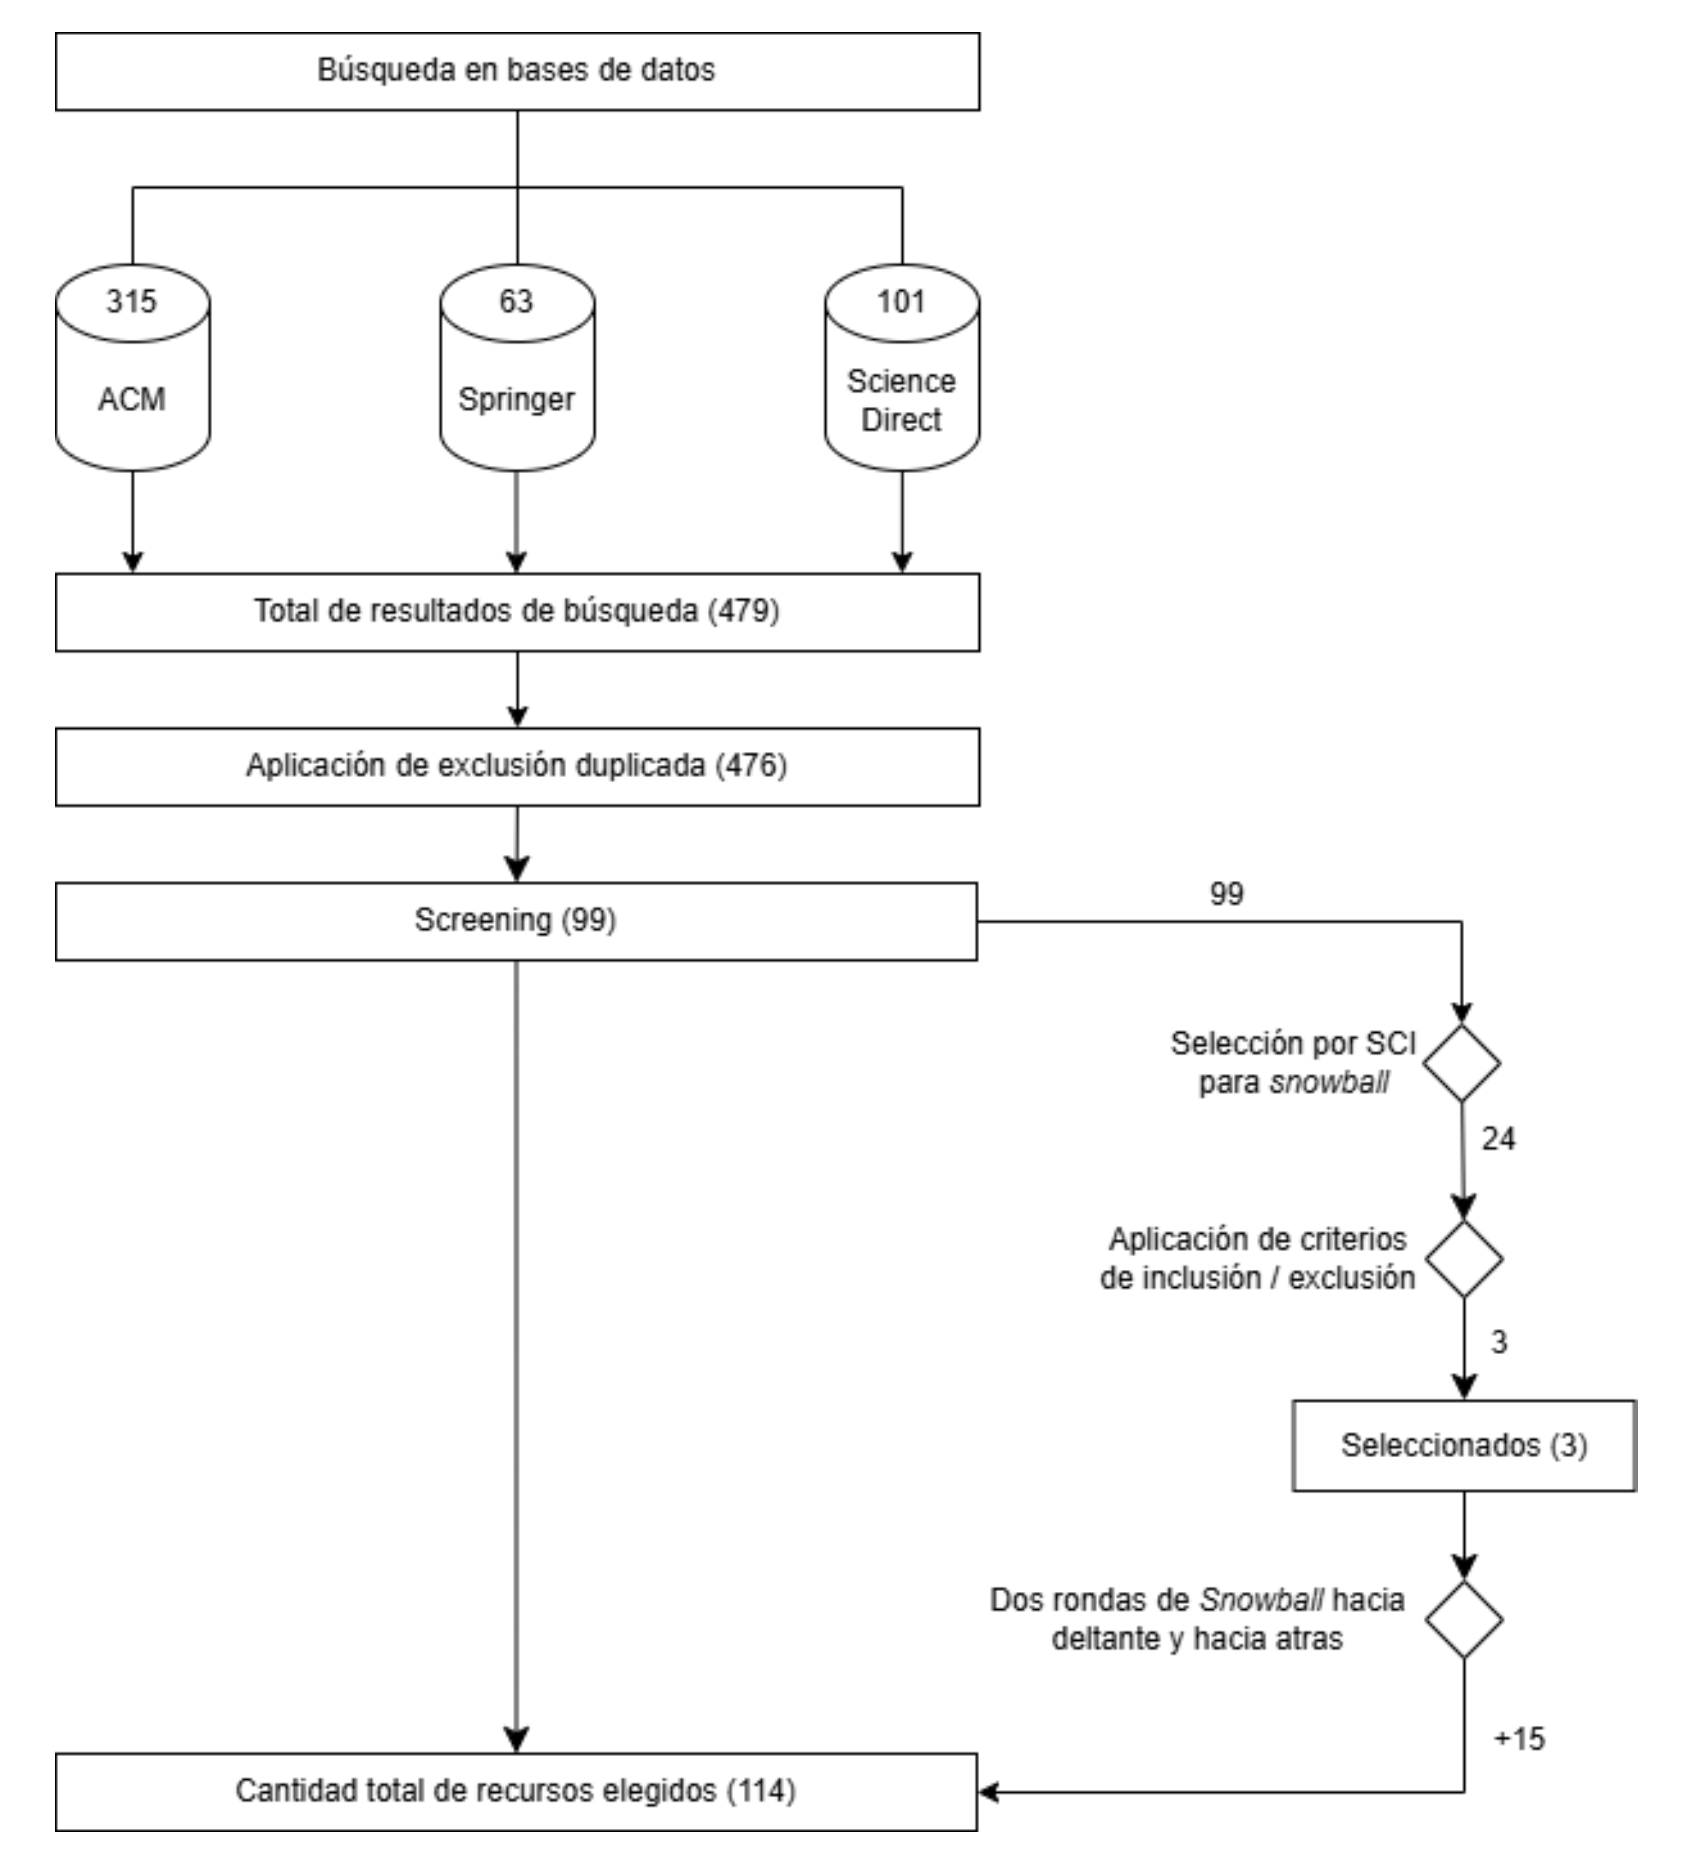
\includegraphics[scale=0.4]{tablas-images/dar/resumen-mapeo.png}
	\caption{Estudio de mapeo sistemático (\SMS).}
	\label{fig:sms}
\end{figure}

La Tabla \ref{tab:aparicion_universos} muestra los resultados del mapeo, donde la primera columna indica el universo, la segunda los códigos de los artículos relacionados con dicho universo, y la tercera el conteo total de artículos por Universo.

\begin{table}[H]
	\centering
	\renewcommand{\arraystretch}{1.2} % Espaciado reducido
	\fontsize{9pt}{10pt}\selectfont % Tamaño de fuente 8pt
	\caption{Aparición de universos en la literatura.}
	\label{tab:aparicion_universos}
	\begin{tabular}{|l|p{8cm}|c|}
		\hline
		\textbf{Universo} & \textbf{SPS ID (Estudios)}                                                                                                                                                                                                                                                                                                                                                                       & \textbf{Suma por Universo} \\
		\hline
		Parallel          & \tiny{SPS006 SPS007 SPS009 SPS010 SPS013 SPS017 SPS021 SPS024 SPS025 SPS026 SPS032 SPS034 SPS035 SPS037 SPS038 SPS041 SPS042 SPS043 SPS044 SPS045 SPS046 SPS049 SPS050 SPS054 SPS061 SPS065 SPS066 SPS068 SPS070 SPS071 SPS072 SPS073 SPS074 SPS075 SPS077 SPS079 SPS080 SPS082 SPS083 SPS084 SPS085 SPS092 SPS093 SPS094 SPS096 SPS101 SPS103 SPS104 SPS105 SPS106 SPS109 SPS110 SPS111 SPS112} & 54                         \\
		\hline
		Vanilla           & \tiny{SPS016 SPS017 SPS018 SPS020 SPS027 SPS028 SPS029 SPS031 SPS032 SPS033 SPS039 SPS044 SPS045 SPS047 SPS049 SPS050 SPS058 SPS063 SPS067 SPS070 SPS076 SPS078 SPS080 SPS086 SPS087 SPS088 SPS089 SPS090 SPS095 SPS097 SPS099 SPS102 SPS108 SPS109 SPS111 SPS113 SPS103}                                                                                                                        & 37                         \\
		\hline
		Container         & \tiny{SPS004 SPS011 SPS019 SPS025 SPS026 SPS034 SPS035 SPS037 SPS038 SPS044 SPS053 SPS080 SPS081 SPS084 SPS085 SPS108}                                                                                                                                                                                                                                                                           & 16                         \\
		\hline
		Grid              & \tiny{SPS001 SPS002 SPS003 SPS005 SPS006 SPS008 SPS009 SPS014 SPS015 SPS017 SPS018 SPS028 SPS029 SPS040 SPS046 SPS048 SPS052 SPS053 SPS055 SPS057 SPS060 SPS061 SPS062 SPS064 SPS065 SPS066 SPS069 SPS074 SPS075 SPS087 SPS089 SPS090 SPS091 SPS092 SPS098 SPS100 SPS107 SPS112 SPS114}                                                                                                          & 39                         \\
		\hline
		Docker            & \tiny{SPS004 SPS019 SPS036 SPS053 SPS085}                                                                                                                                                                                                                                                                                                                                                        & 5                          \\
		\hline
		Java              & \tiny{SPS043}                                                                                                                                                                                                                                                                                                                                                                                    & 1                          \\
		\hline
	\end{tabular}
\end{table}

\subsection{Análisis DAR}
Con los criterios definidos y la medición de popularidad completada, se procedió a realizar el análisis DAR, cuyos resultados se presentan en la Tabla \ref{tab:analisis_dar}.

\begin{table}[H]
	\centering
	\renewcommand{\arraystretch}{1.2} % Espaciado reducido
	\fontsize{9pt}{10pt}\selectfont % Tamaño de fuente 8pt
	\caption{Análisis DAR.}
	\label{tab:analisis_dar}
	\begin{tabular}{|>{\centering\arraybackslash}p{1.8cm}|>{\centering\arraybackslash}p{1.8cm}|>{\centering\arraybackslash}p{2.5cm}|>{\centering\arraybackslash}p{2.2cm}|>{\centering\arraybackslash}p{0.7cm}|>{\centering\arraybackslash}p{1.4cm}|>{\centering\arraybackslash}p{1.5cm}|}
		\hline
		{\scriptsize\textbf{Criterio}}                         & {\tiny\textbf{PARALLEL}}                                                   & {\tiny\textbf{CHECKPOINTING}}                          & {\tiny\textbf{POPULARITY}} & {\tiny\textbf{DOC}} & {\tiny\textbf{ROLE DIV}} & {\tiny\textbf{}}            \\
		\hline
		{\cellcolor[HTML]{E6E6E6}\scriptsize\textbf{Universo}} & \multicolumn{5}{c|}{\cellcolor[HTML]{E6E6E6}{\scriptsize\textbf{Puntaje}}} & \cellcolor[HTML]{E6E6E6}{\scriptsize\textbf{Promedio}}                                                                                                             \\
		\hline
		Vanilla                                                & 1                                                                          & 3                                                      & 3                          & 3                   & 3                        & \cellcolor[HTML]{DBF7FF}2,6 \\
		\hline
		Grid                                                   & 2                                                                          & 3                                                      & 3                          & 2                   & 3                        & \cellcolor[HTML]{FFCCC2}2,6 \\
		\hline
		Java                                                   & 1                                                                          & 3                                                      & 1                          & 1                   & 3                        & 1,8                         \\
		\hline
		Scheduler                                              & 1                                                                          & 3                                                      & 1                          & 1                   & 3                        & 1,8                         \\
		\hline
		Local                                                  & 1                                                                          & 3                                                      & 1                          & 1                   & 1                        & 1,4                         \\
		\hline
		Parallel                                               & 3                                                                          & 1                                                      & 3                          & 3                   & 3                        & \cellcolor[HTML]{FFCCC2}2,6 \\
		\hline
		VM                                                     & 1                                                                          & 3                                                      & 3                          & 1                   & 3                        & 2,2                         \\
		\hline
		Container                                              & 1                                                                          & 3                                                      & 1                          & 1                   & 3                        & 1,8                         \\
		\hline
		Docker                                                 & 1                                                                          & 3                                                      & 1                          & 1                   & 3                        & 1,8                         \\
		\hline
	\end{tabular}
	\vspace{5pt}
\end{table}

\section{Resultados}

\subsection{Resumen del análisis}
El proceso ejecutado tuvo como fin tomar una decisión informada sobre el Universo a implementar en la infraestructura HTCondor del \GRID. Considerando el resultado descrito en la Tabla \ref{tab:analisis_dar}, hubo un empate en los Universos ganadores \textbf{Grid } y \textbf{Parallel}. Teniendo en cuenta esta situación que no se tenía en cuenta desde el principio, se tomó la decisión de continuar con las demás etapas del proyecto con ambos Universos, ya que no hay motivos, razones ni evidencia para orientarse o preferir uno sobre otro.

Grosso modo, el Universo Grid funciona como un middleware o intermediario que hace de puente para enviar trabajos computacionales desde un nodo submit hacia un pool HTCondor de recursos externos. Por su parte, el Universo Parallel ejecuta programas que hacen usos de alguna implementación de \MPI como OpenMPI para lograr así una ejecución sincronizada y ordenada con el fin de permitir la comunicación entre los nodos.

\subsection{Próximos pasos}
Se procederá con el diseño de las arquitecturas de la solución con cada Universo y su posterior implementación a través de un prototipo funcional.
 % TODO
\ChapterImageStar[cap:disenio]{Diseño de la solución}{./images/fondo.png}\label{cap:disenio}
\mbox{}\\

El presente capítulo tiene como objetivo fundamental traducir la decisión estratégica —la implementación de los Universos Grid y Parallel— en un diseño técnico y estratégico concreto y ejecutable. Aquí se especifica la arquitectura de la solución, detallando los componentes de HTCondor que serán configurados o modificados, los flujos de trabajo establecidos para cada universo y los criterios de interoperabilidad con el Universo Vanilla preexistente. Este diseño busca establecer las bases técnicas y metodológicas para la fase de implementación, propendiendo por la robustez, escalabilidad e integridad de la infraestructura de computación distribuida resultante. Además, busca ayudar al Grupo \GRID con el cumplimiento de sus objetivos estratégicos y el cierre de la brecha identificada en la caracterización.

\section{Definición de estrategia}
La definición de la estrategia de diseño se fundamenta en una filosofía de desarrollo guiado por pruebas (\TDD), que es una disciplina de diseño y programación donde cada línea de código está escrita en respuesta a una prueba que el programador escribe justo antes de escribir el código \citep{4163024}. Antes de especificar los componentes arquitectónicos, se establece un conjunto de casos de prueba estructurados que definen de manera formal y verificable el comportamiento esperado de los Universos \textit{Grid} y \textit{Parallel}. Estos casos, que funcionan como criterios de aceptación guiarán de manera iterativa el diseño de la solución, asegurando que cada decisión de implementación esté directamente alineada con la validación funcional del sistema.

Por último, se considera necesario establecer un nombre para el sistema. Esto con el fin de dar mayor claridad al lector y hacer más visibles los momentos en los que se habla del sistema resultado de este proyecto. Se opta por el "Grid App" haciendo referencia al Grupo \GRID, que es el sujeto nuclear de este proyecto; al Universo Grid, que es uno de los Universos que se decidió implementar para este proyecto de aplicación después de la toma de decisiones estructurada mediante el análisis \DAR y el modelo computacional Grid que es básicamente una infraestructura que provee gran capacidad computacional a un sistema distribuido haciendo uso de recursos geográficamente distribuidos \citep{8974490}.

\section{Casos de prueba}

\subsection{Definición de requisitos}
\noindent
Para iniciar con la definición de casos de prueba, se establecen los requisitos que debe cumplir \textit{Grid App} que están fundamentados en el análisis preliminar hecho anteriormente, principalmente en la descripción de la oportunidad para el Grupo \GRID.

\subsubsection{Requisitos funcionales}
\noindent
Según \cite{159342} un requisito funcional especifica una función que el sistema o que un componente del sistema es capaz de hacer. A continuación se definen los requisitos funcionales para \textit{Grid App}.
\begin{table}[H]
	\centering
	\sffamily\scriptsize
	\setlength{\tabcolsep}{4pt}
	\renewcommand{\arraystretch}{1.3}
	\caption{Requisitos funcionales para \textit{Grid App}}
	\label{table:requisitosFuncionales}
	\begin{tabular}{|p{0.1\textwidth}|p{0.2\textwidth}|p{0.7\textwidth}|}
		\toprule
		\textbf{ID}                              & \textbf{Título}                               & \textbf{Descripción} \\
		\midrule
		RF1 & Soporte para Universos adicionales & El sistema debe permitir la ejecución de trabajos en al menos dos Universos adicionales a Vanilla (Grid y Parallel) \\
		\midrule
		RF2 & Orquestación de múltiples clústeres & El sistema debe permitir enviar trabajos hacia diferentes clústeres (Parallel, Vanilla) a través del Universo Grid. \\
		\midrule
		RF3 & Selección de destino & El sistema debe permitir que el usuario especifique el clúster de destino. \\
		\midrule
		RF4 & Monitoreo de trabajos & El sistema debe permitir el monitoreo de los trabajos enviados a los clústeres, mostrando su estado al usuario. \\
		\midrule
		RF5 & Ejecución MPI en Parallel & Un clúster debe soportar ejecución de trabajos basados en MPI en múltiples nodos (≥ N nodos configurados). \\
		\midrule
		RF6 & Redirección Grid-Parallel & El Grid Manager debe aceptar trabajos enviados al Universo Grid y, si la naturaleza del trabajo es paralelo, redirigirlos correctamente al Universo Parallel. \\
        \midrule
		RF7 & Redirección Grid-Vanilla & El Grid Manager debe aceptar trabajos enviados al Universo Grid y, si la naturaleza del trabajo es distribuido, redirigirlos correctamente al Universo Vanilla. \\
        \midrule
		RF8 & Registro centralizado de errores & El Grid Manager debe centralizar \textit{logs} de fallos de ejecución provenientes de cada clúster. \\
		\bottomrule
	\end{tabular}
\end{table}

\subsubsection{Requisitos no-funcionales}
\noindent
Según \cite{4384163} un requisito no-funcional es un atributo o una restricción de un sistema. A continuación se definen los requisitos no-funcionales para \textit{Grid App}.
\begin{table}[H]
	\centering
	\sffamily\scriptsize
	\setlength{\tabcolsep}{4pt}
	\renewcommand{\arraystretch}{1.3}
	\caption{Requisitos no-funcionales para \textit{Grid App}}
	\label{table:requisitosNoFuncionales}
	\begin{tabular}{|p{0.1\textwidth}|p{0.2\textwidth}|p{0.7\textwidth}|}
		\toprule
		\textbf{ID}                              & \textbf{Título}                               & \textbf{Descripción} \\
		\midrule
		RNF1 & Transparencia de uso & El usuario no debe preocuparse por las configuraciones internas de cada clúster; el Grid Manager abstrae el destino mediante una interfaz más amigable. \\
		\midrule
		RNF2 & Usabilidad & La configuración de los nuevos Universos debe estar documentada y ser accesible mediante manual de despliegue para los usuarios del Grupo GRID. \\
		\midrule
		RNF3 & Disponibilidad & En caso de que un clúster esté inactivo, el Grid Manager debe registrar el error y permitir redirección a otro clúster disponible si el Universo es compatible. \\
		\bottomrule
	\end{tabular}
\end{table}

\subsection{Pruebas}
\noindent
Para esta sección, se definen las pruebas y los pasos para ejecutar cada prueba.
\begin{table}[H]
	\centering
	\renewcommand{\arraystretch}{1.2} % Espaciado reducido
	\fontsize{9pt}{10pt}\selectfont % Tamaño de fuente 8pt
	\begin{tabular}{|p{2cm}|p{4cm}|p{2.5cm}|p{4.7cm}|} % Total: 14cm
		\hline
		\textbf{ID del escenario de pruebas}    & ESC-01                                                                              & \textbf{ID de requisito}        & RF1, RF2, RF3, RF4, RF7, RF8, RNF1, RNF2, RNF3                      \\
		\textbf{Título de la prueba}            & Ejecución de trabajos en Universo Grid con repeticiones de iguales parámetros       & \textbf{Prerrequisitos}         & Grid Manager configurado con al menos un clúster soportando Vanilla \\
		\textbf{Descripción del caso de prueba} & Validar que el sistema soporta ejecución en Universo Grid hacia el Universo Vanilla & \textbf{Prioridad de la prueba} & Alta                                                                \\
		\hline
		\multicolumn{4}{|c|}{\textbf{Pasos de ejecución de las pruebas}}                                                                                                                                                                      \\
		\hline
		\textbf{ID de paso}                     & \textbf{Acción}                                                                     & \textbf{Datos de prueba}        & \textbf{Resultado esperado}                                         \\
		1                                       & Ingresar a la página                                                                & Link de la aplicación           & Página principal de la aplicación mostrada                          \\
		2                                       & Subir binario a través del selector de archivos                                     & Binario de ejecución            & Binario almacenado en el sistema de envío                           \\
		3                                       & Escribir argumentos adicionales (Opcional)                                          & Argumentos adicionales          & Argumentos seteados en el submit file dinámico                      \\
		4                                       & Seleccionar la naturaleza del trabajo (Distribuido)                                 & Naturalezas permitidas          & Universo seteado en el submit file dinámico                         \\
		5                                       & Seleccionar la información de distribución (Repeticiones con mismos parámetros)     & Distribuciones permitidas       & Agregada estructura necesaria al Submit file                        \\
		6                                       & Seleccionar cantidad de repeticiones                                                & Repeticiones necesarias         & Ciclo de envío en el archivo de shell creado                        \\
		7                                       & Seleccionar clúster más favorable                                                   & Métricas de clústeres           & Recurso remoto del grid en el submit file establecido               \\
		8                                       & Enviar trabajo                                                                      & Submit file generado            & Shell de envío y submit file ejecutado                              \\
		9                                       & Ver resultados a medida que van terminando                                          & Resultados de trabajos          & Salida de cada ejecución mostrada de forma organizada               \\
		\hline
	\end{tabular}
	\caption{Información ESC-01}
	\label{table:esc-01}
\end{table}

\begin{table}[H]
	\centering
	\renewcommand{\arraystretch}{1.2} % Espaciado reducido
	\fontsize{9pt}{10pt}\selectfont % Tamaño de fuente 8pt
	\begin{tabular}{|p{2cm}|p{4cm}|p{2.5cm}|p{4.7cm}|} % Total: 14cm
		\hline
		\textbf{ID del escenario de pruebas}    & ESC-02                                                                              & \textbf{ID de requisito}        & RF1, RF2, RF3, RF4, RF7, RF8, RNF1, RNF2, RNF3                      \\
		\textbf{Título de la prueba}            & Ejecución de trabajos en Universo Grid con variables parametrizables                & \textbf{Prerrequisitos}         & Grid Manager configurado con al menos un clúster soportando Vanilla \\
		\textbf{Descripción del caso de prueba} & Validar que el sistema soporta ejecución en Universo Grid hacia el Universo Vanilla & \textbf{Prioridad de la prueba} & Alta                                                                \\
		\hline
		\multicolumn{4}{|c|}{\textbf{Pasos de ejecución de las pruebas}}                                                                                                                                                                      \\
		\hline
		\textbf{ID de paso}                     & \textbf{Acción}                                                                     & \textbf{Datos de prueba}        & \textbf{Resultado esperado}                                         \\
		1                                       & Ingresar a la página                                                                & Link de la aplicación           & Página principal de la aplicación mostrada                          \\
		2                                       & Subir binario a través del selector de archivos                                     & Binario de ejecución            & Binario almacenado en el sistema de envío                           \\
		3                                       & Escribir argumentos adicionales (Opcional)                                          & Argumentos adicionales          & Argumentos seteados en el submit file dinámico                      \\
		4                                       & Seleccionar la naturaleza del trabajo (Distribuido)                                 & Naturalezas permitidas          & Universo seteado en el submit file dinámico                         \\
		5                                       & Seleccionar la información de distribución (Repeticiones con mismos parámetros)     & Distribuciones permitidas       & Agregada estructura necesaria al Submit file                        \\
		6                                       & Seleccionar variable parametrizable (De los argumentos adicionales)                 & Variables parametrizables       & Ciclo de envío en el archivo de shell creado                        \\
		7                                       & Establecer valor inicial                                                            & Valor inicial                   & Valor inicial del ciclo establecido                                 \\
		8                                       & Establecer valor final                                                              & Valor final                     & Valor final del ciclo establecido                                   \\
		9                                       & Establecer incremento                                                               & Incremento                      & Incremento del ciclo establecido                                    \\
		10                                      & Ver cantidad de repeticiones                                                        & Repeticiones necesarias         & Cantidad de repeticiones calculadas                                 \\
		11                                      & Seleccionar clúster más favorable                                                   & Métricas de clústeres           & Recurso remoto del grid en el submit file establecido               \\
		12                                      & Enviar trabajo                                                                      & Submit file generado            & Shell de envío y submit file ejecutado                              \\
		13                                      & Ver resultados a medida que van terminando                                          & Resultados de trabajos          & Salida de cada ejecución mostrada de forma organizada               \\
		\hline
	\end{tabular}
	\caption{Información ESC-02}
	\label{table:esc-02}
\end{table}

\begin{table}[H]
	\centering
	\renewcommand{\arraystretch}{1.2} % Espaciado reducido
	\fontsize{9pt}{10pt}\selectfont % Tamaño de fuente 9pt
	\begin{tabular}{|p{2cm}|p{4cm}|p{2.5cm}|p{4.7cm}|} % Total: 14cm
		\hline
		\textbf{ID del escenario de pruebas}    & ESC-03                                                        & \textbf{ID de requisito}        & RF1, RF2, RF3, RF4, RF5, RF6, RF8, RNF1, RNF2, RNF3                        \\
		\textbf{Título de la prueba}            & Ejecución de trabajos en Universo Parallel                    & \textbf{Prerrequisitos}         & Grid Manager configurado con al menos un clúster soportando Parallel       \\
		\textbf{Descripción del caso de prueba} & Validar que el sistema soporta ejecución en Universo Parallel & \textbf{Prioridad de la prueba} & Alta                                                                       \\
		\hline
		\multicolumn{4}{|c|}{\textbf{Pasos de ejecución de las pruebas}}                                                                                                                                                       \\
		\hline
		\textbf{ID de paso}                     & \textbf{Acción}                                               & \textbf{Datos de prueba}        & \textbf{Resultado esperado}                                                \\
		\hline
		1                                       & Ingresar a la página                                          & Link de la aplicación           & Página principal de la aplicación mostrada                                 \\
		2                                       & Subir binario a través del selector de archivos               & Binario de ejecución            & Binario almacenado en el sistema de envío                                  \\
		3                                       & Escribir argumentos adicionales (Opcional)                    & Argumentos adicionales          & Argumentos establecidos en el \textit{submit file} dinámico                \\
		4                                       & Seleccionar la naturaleza del trabajo (Paralelo)              & Naturalezas permitidas          & Universo establecido en el \textit{submit file} dinámico                   \\
		5                                       & Escribir cantidad de máquinas requeridas                      & Máquinas requeridas             & Parámetro ``\textit{machine\_count}'' del \textit{submit file} establecido \\
		6                                       & Escribir cantidad de núcleos solicitados por máquina          & Núcleos requeridos              & Parámetro ``\textit{required\_cpus}'' del \textit{submit file} establecido \\
		7                                       & Seleccionar clúster más favorable                             & Métricas de clústeres           & Recurso remoto establecido                                                 \\
		8                                       & Enviar trabajo                                                & \textit{Submit file} generado   & \textit{Script} de envío y \textit{submit file} ejecutado                  \\
		9                                       & Ver resultados a medida que van terminando                    & Resultados de trabajos          & Salida de cada ejecución mostrada de forma organizada                      \\
		\hline
	\end{tabular}
	\caption{Información ESC-03}
	\label{table:esc-03}
\end{table}


\subsection{Casos de uso}
\noindent
Luego de tener las pruebas que se van a ejecutar al sistema \textit{Grid App} ya definidas, se procede con la creación de un caso de uso por cada prueba. Esto tiene 3 motivaciones en este trabajo; (1) Mostrar la utilidad del sistema para un usuario ficticio, (2) Limitar el alcance del prototipo a unos casos de uso concretos y (3) Guiar el desarrollo hacia situaciones reales y la utilidad para los \textit{stakeholders}.

A continuación se definen los casos de uso:

\subsubsection{Caso 1: Montecarlo para pi}
\noindent
\begin{itemize}
    \item \textbf{Descripción:} En un laboratorio de investigación financiera, los analistas necesitan valuar instrumentos derivados complejos utilizando métodos Montecarlo que requieren cientos de simulaciones. La infraestructura \HTCondor distribuye estos cálculos estadísticos masivos a través de múltiples nodos, donde cada trabajo ejecuta una porción de las simulaciones para calcular aproximaciones de pi como prototipo, y luego consolida los resultados para obtener una mejor estimación que valide la confiabilidad del sistema en modelos de riesgo financiero.
    \item \textbf{Escenario de prueba relacionado:} ESC-01
\end{itemize}

\subsubsection{Caso 2: Conteo de números primos}
\noindent
\begin{itemize}
    \item \textbf{Descripción:} Un centro de criptografía debe analizar la distribución de números primos en intervalos grandes para evaluar la seguridad de algoritmos de encriptación RSA. \HTCondor divide automáticamente estos rangos numéricos en sub intervalos que distribuye entre nodos heterogéneos, permitiendo el conteo concurrente de primos que demuestra la capacidad del sistema para manejar cargas computacionales intensivas.
    \item \textbf{Escenario de prueba relacionado:} ESC-02
\end{itemize}

\subsubsection{Caso 3: \textit{Quick-sort} Paralelo}
\noindent
\begin{itemize}
    \item \textbf{Descripción:} Un instituto de genómica requiere ordenar cantidades enormes de datos de secuencias de ADN para identificar patrones de mutaciones genéticas. El algoritmo de \textit{quick-sort} paralelo implementado con \MPI aprovechar los recursos agregados de memoria y procesamiento de múltiples máquinas bajo \HTCondor, validando la capacidad de la infraestructura para coordinar trabajos que necesitan comunicación entre procesos (\IPC) en aplicaciones científicas.
    \item \textbf{Escenario de prueba relacionado:} ESC-03
\end{itemize}

\section{Modelado del sistema en Archimate}
ArchiMate es un lenguaje de modelado estándar, abierto e independiente de~\textit{The Open Group} que permite representar de manera estructurada y general las diferentes capas de una arquitectura empresarial: negocio, aplicación y tecnología \citep{josey2016introduction}. Esto permite tener una visión integrada que facilita la comunicación entre los distintos actores de un negocio y que muestre cómo los procesos, los sistemas de información y la infraestructura tecnológica se relacionan entre sí.
A su vez, Archi es un Software que permite realizar diagramas de ArchiMate de forma sencilla y fue el Software elegido por el equipo de este proyecto para modelar las relaciones del proyecto con el negocio y varios elementos más. Archi permite dividir los modelos en vistas, que facilitan la organización y hacen más sencilla la labor de ampliar ciertos elementos o modelos importantes.

Cabe recalcar que algunos de los elementos como la misión y la visión no se muestran de forma completa en las vistas debido a su gran extensión textual. Sin embargo, con el fin de mostrar información completa, se mencionan y describen a continuación.

\begin{itemize}
    \item \textbf{Misión:} El Grupo de Investigación en Redes, Información y Distribución - GRID tiene como objetivo principal la realización de proyectos de investigación en temas relacionados principalmente con soluciones informáticas en Infraestructura Computacional, la Ingeniería de Software, el Análisis de Datos y la Informática Educativa. Hacer investigación en los temas mencionados, así como realizar proyectos interdisciplinarios deberá redundar en conocimientos frescos y la adopción de nuevas tecnologías que contribuyan al desarrollo académico del Programa Ingeniería de Sistemas y Computación, la Maestría en Ingeniería, y la Maestría y el Doctorado en Educación de la Universidad del Quindío. Luego de 10 años de existencia, de haber superado exitosamente los procesos de formación a nivel doctoral y de maestría de nuestros integrantes y de haber logrado la categoría C en el escalafón nacional de Ministerio de Ciencia, Tecnología e Innovación, nuestros esfuerzos estarán centrados en: (1) la formación de estudiantes a nivel de pregrado, maestría y doctorado; (2) fortalecer los lazos de amistad y colaboración con investigadores y grupos de investigación a nivel nacional e internacional; (3) la realización de proyectos de investigación y desarrollo de productos de nuevo conocimiento que busquen dar solución a problemas de la sociedad; y (4) aumentar la visibilidad del grupo y mejorar la categoría en el escalafón de MinCiencias.
    \item \textbf{Visión:} Para el año 2025, el Grupo de Investigación en Redes, Información y Distribución - GRID de la Facultad de Ingeniería de la Universidad del Quindío será un grupo consolidado y reconocido en la más alta categoría del escalafón nacional del Ministerio de Ciencia Tecnología e Innovación, que a través de sus aportes sea tenido en cuenta en la toma de decisiones a nivel regional y nacional; y con reconocimiento internacional mediante la realización de trabajos en colaboración con investigadores de otras universidades nacionales y extranjeras. Misión: Somos un grupo de profesores universitarios dedicados a realizar investigación en áreas tecnológicas orientadas a facilitar procesos y resolver problemas de la comunidad académica, de la sociedad que nos rodea y del sector productivo, mediante la adaptación de tecnologías o el desarrollo de soluciones informáticas en Infraestructura Computacional, la Ingeniería de Software, el Análisis de Datos y la Informática Educativa que constituyan un aporte al desarrollo social, económico y tecnológico de la región y el país.
    \item \textbf{Objetivo estratégico 1:} Realizar proyectos de investigación en los temas relacionados con las áreas de interés del grupo, así como proyectos interdisciplinarios que permitan la adopción de conocimientos y nuevas tecnologías que contribuyan al desarrollo de la región, del país y de la comunidad académica mundial.
    \item \textbf{Objetivo estratégico 2:} Establecer contactos con otros grupos de investigación interesados en temáticas similares, pertenecientes a otras instituciones de educación superior, tanto a nivel nacional como internacional.
    \item \textbf{Objetivo estratégico 3:} Impulsar la investigación dentro de la Universidad del Quindío y la Facultad de Ingeniería, particularmente en el programa Ingeniería de Sistemas y Computación, el programa de Maestría en Ingeniería, y los programas de Maestría y Doctorado en Educación.
    \item \textbf{Objetivo estratégico 4:} Establecer una comunidad académica con la participación de estudiantes de pregrado y posgrado, profesores y jóvenes investigadores.
\end{itemize}

\subsection{Vista de misión, visión y objetivos}
\noindent
En la Figura \ref{fig:archiMVOView} se muestra las relaciones entre la misión, la visión y los objetivos estratégicos del negocio. Además, se muestran los ámbitos clave en los que se enfoca el negocio para cumplir con sus objetivos estratégicos. Esta última información se tomó de conversaciones informales con el representante del negocio para este proyecto, quien manifestó que estos son los enfoques que se le debe dar al proyecto y están dados por la organización a la que está adscrito el negocio, que para nuestro caso específico es el Grupo \GRID.

\begin{figure}[H]
	\centering
	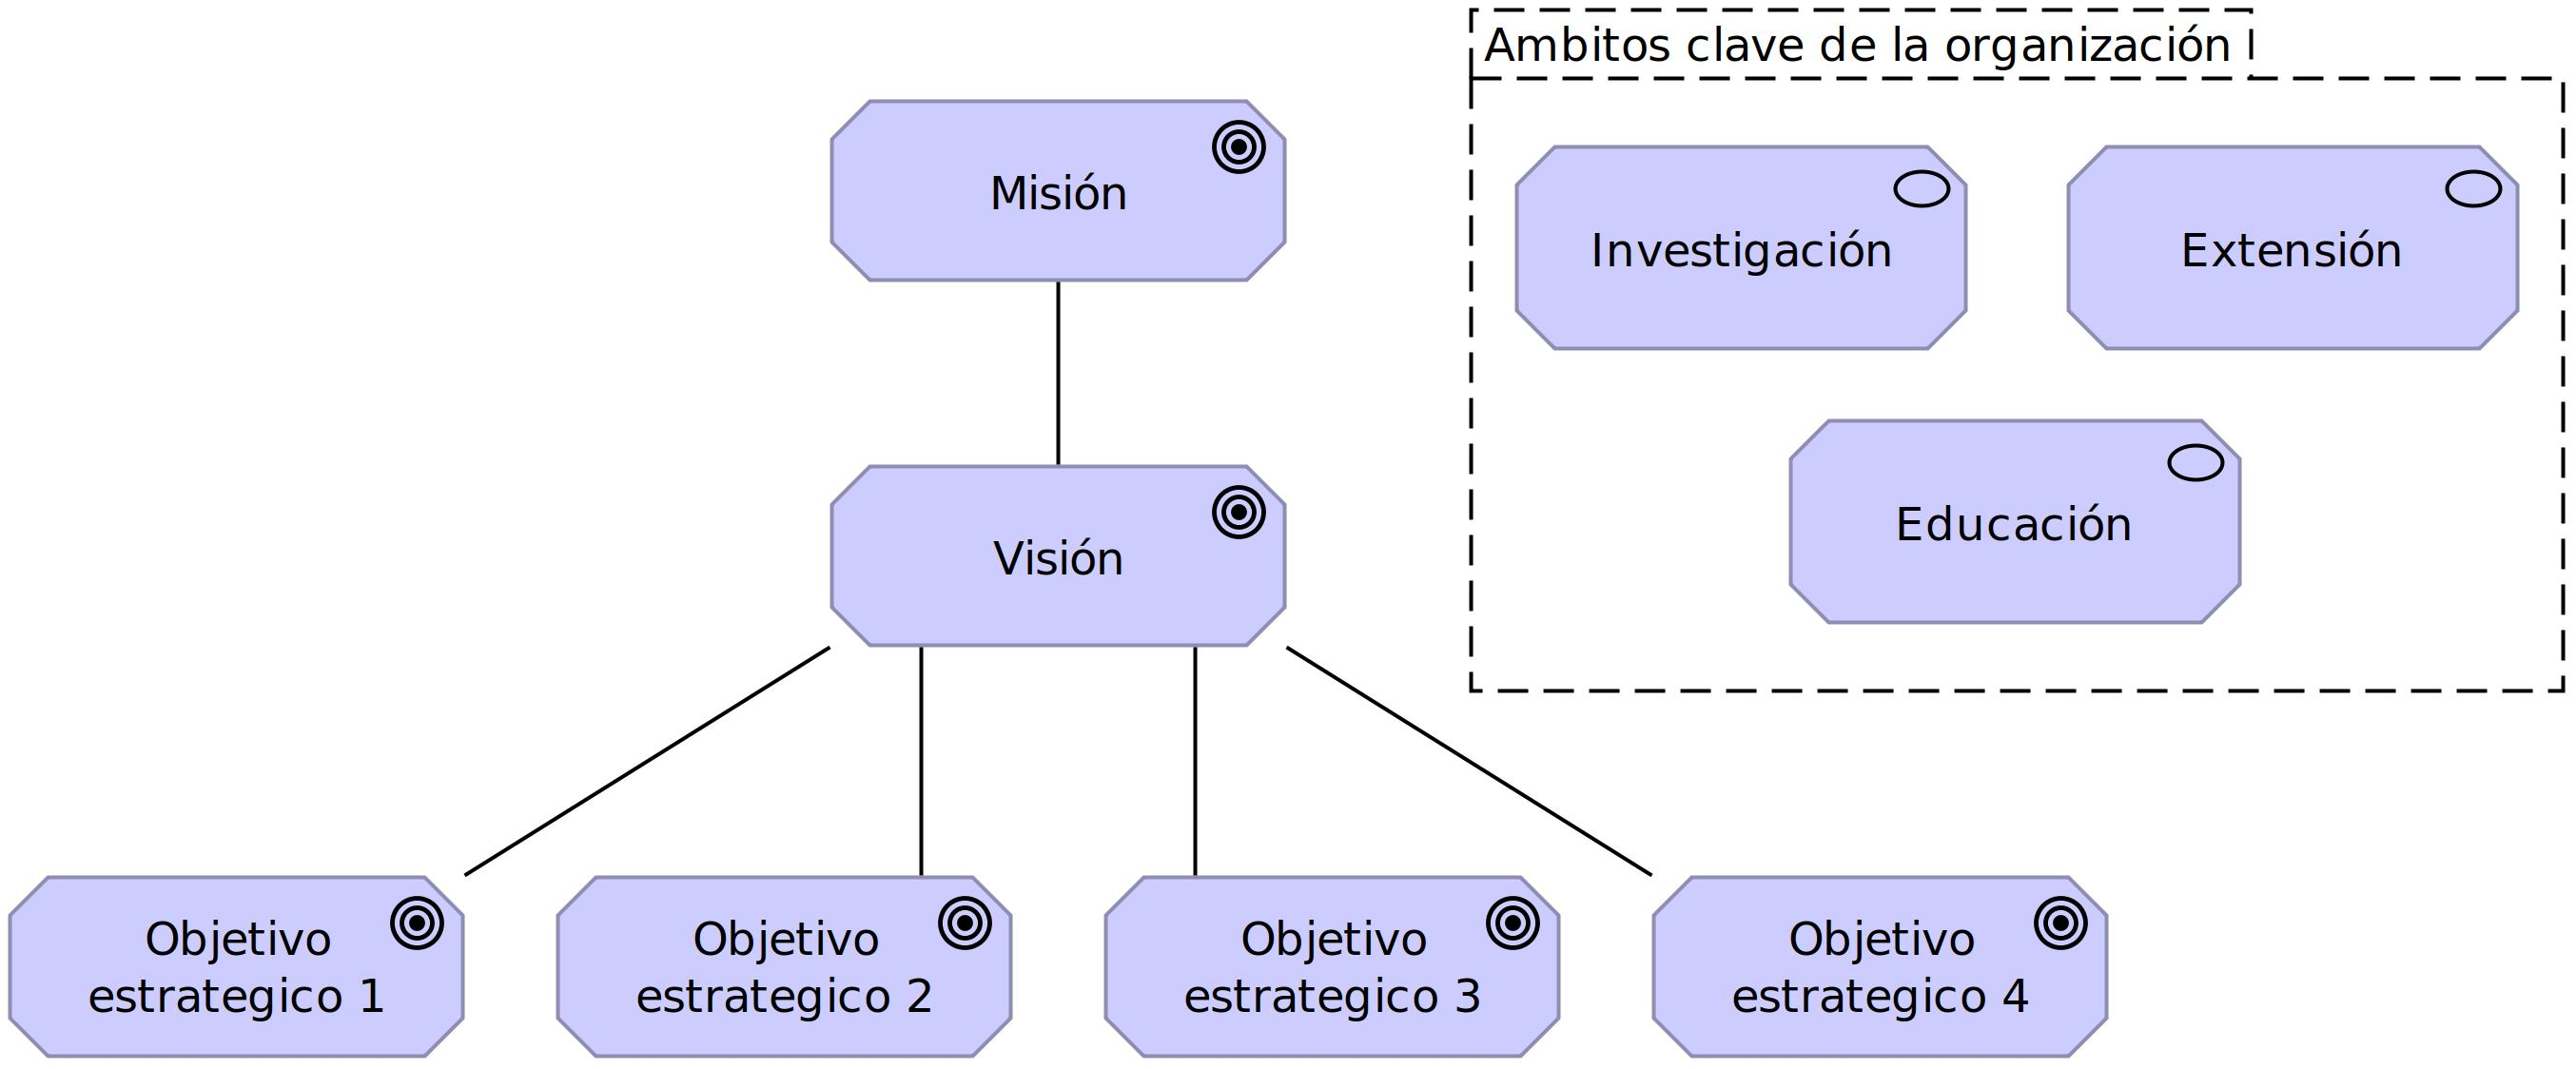
\includegraphics[scale=0.15]{tablas-images/archi/Mission-Values-Vision View.jpg}
	\caption{Vista de misión, visión y objetivos}
    \label{fig:archiMVOView}
\end{figure}

\subsection{Vista de mapa de valor estratégico}
\noindent
En la Figura \ref{fig:archiSVMView} se muestra el valor estratégico del negocio desde distintas perspectivas y su descomposición hacia otros valores más concretos. Todo esto con el fin de conocer que perspectivas son de más interés para el negocio y cuáles valores componen dichas perspectivas. Esto ocurre en capa de motivación, por lo que estos valores estratégicos identificados servirán como los principios orientadores de la estrategia del negocio.

\begin{figure}[H]
	\centering
	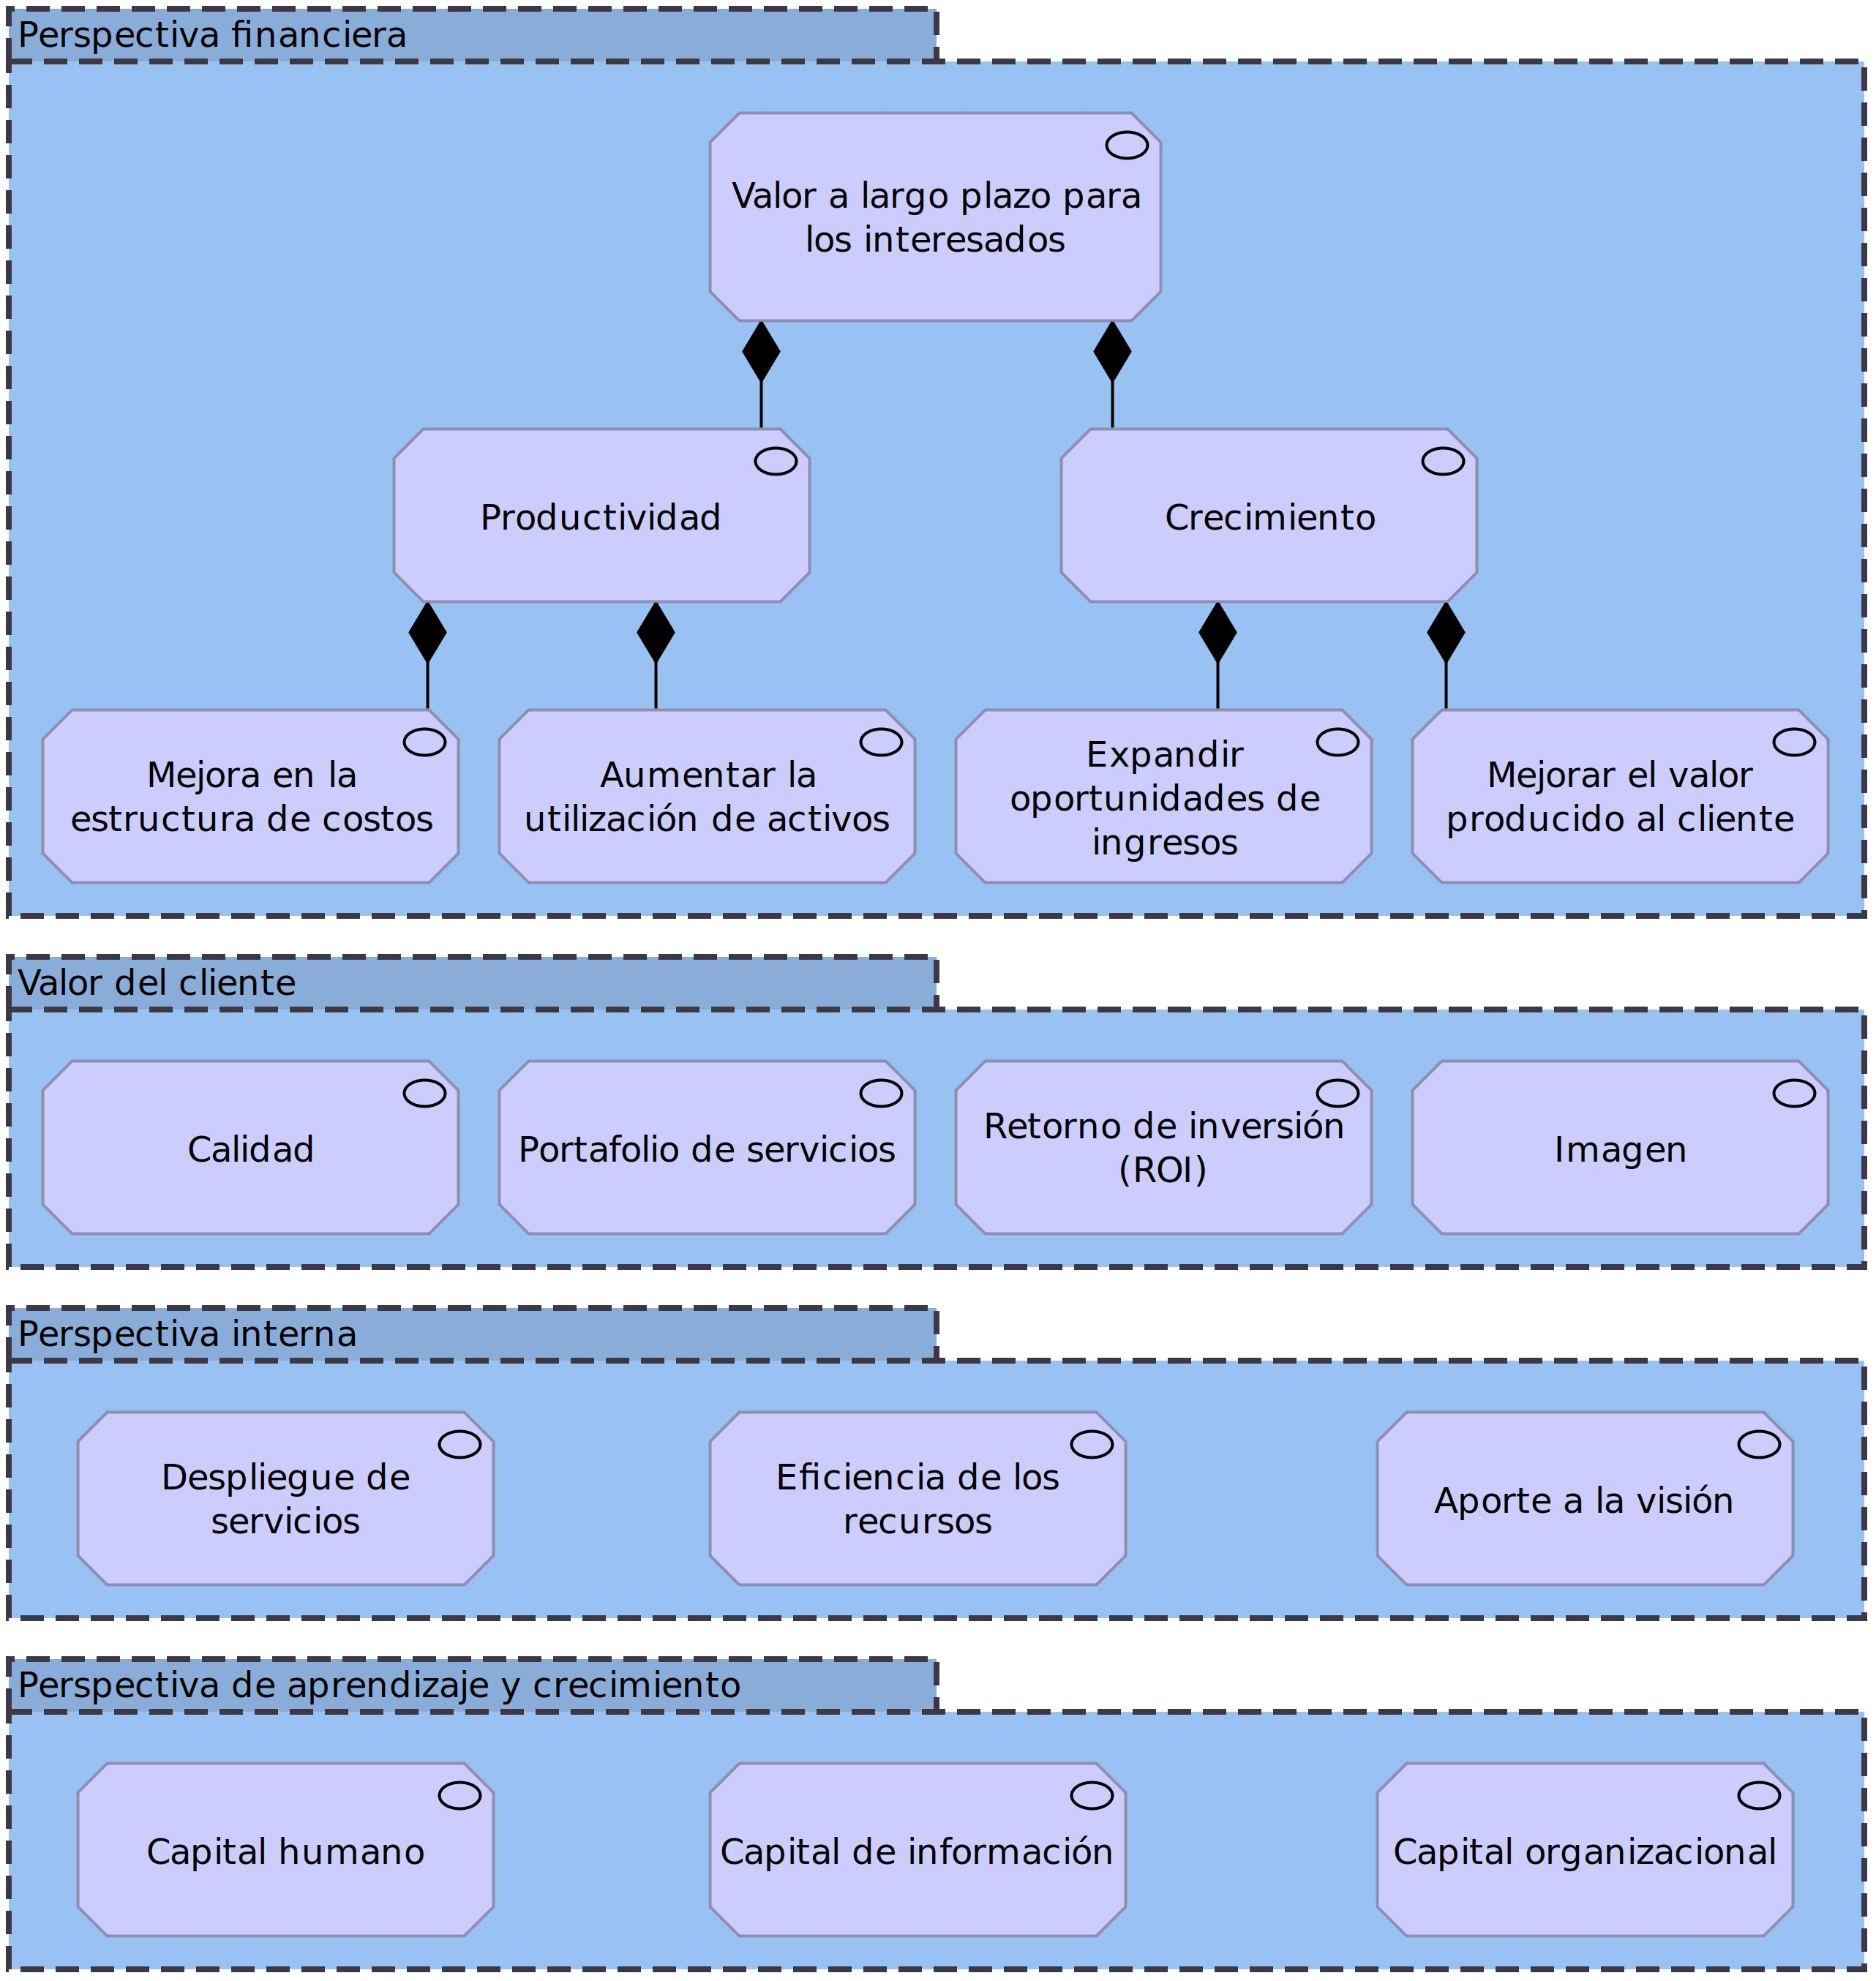
\includegraphics[scale=0.15]{tablas-images/archi/Strategic Value Map View.jpg}
	\caption{Vista de mapa de valor estratégico}
    \label{fig:archiSVMView}
\end{figure}

\subsection{Vista de objetivos}
\noindent
En la Figura \ref{fig:archiGoalsView} se muestra un desglose completo de los objetivos del negocio. Para este fin se usó una variación de una estrategia conocida como 5W, que usa cinco preguntas para obtener información completa sobre un elemento. Estas preguntas son: ¿Quién?, ¿Qué?, ¿Cuándo?, ¿Dónde? Y ¿Por qué? \citep{5WAmitava}. Para el desglose de los objetivos del negocio en esta vista del modelo se hizo necesarias solo cuatro preguntas como se muestra en la Figura \ref{fig:archiGoalsView}. Así, podemos ver como está compuesta la motivación del negocio y los elementos que están en torno a los objetivos estratégicos.

\begin{figure}[H]
	\centering
	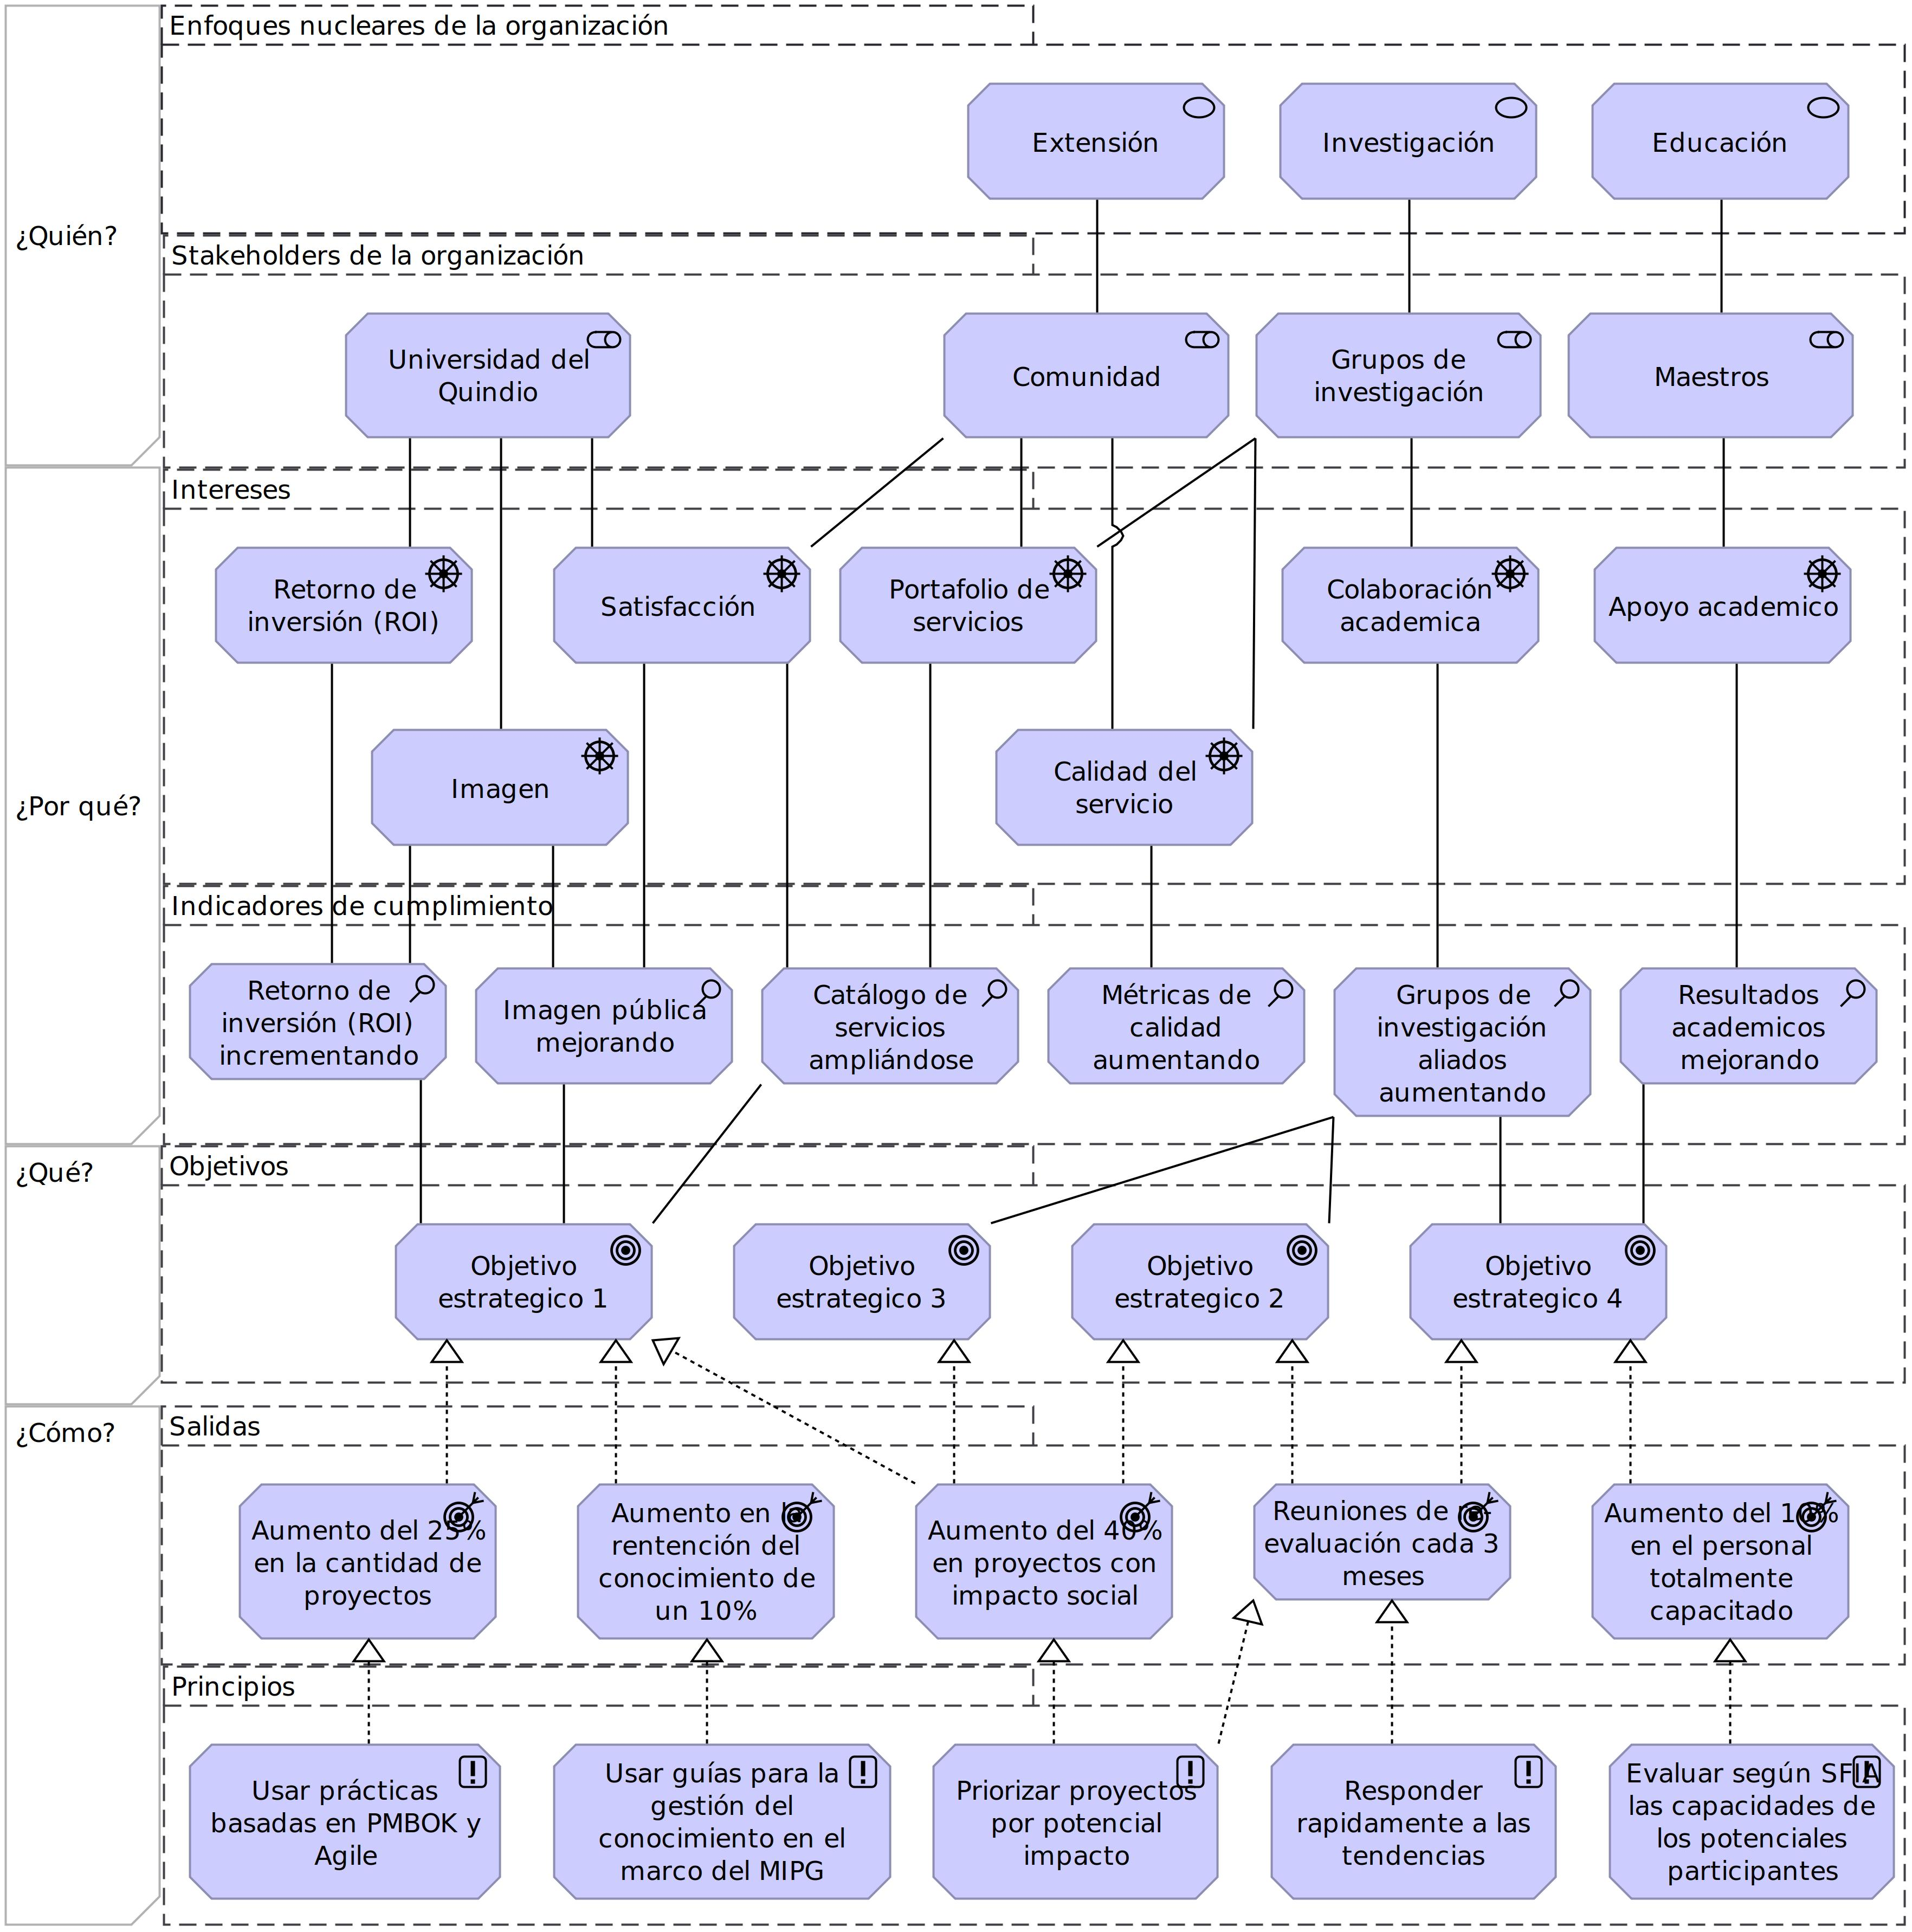
\includegraphics[scale=0.12]{tablas-images/archi/Goals View.jpg}
	\caption{Vista de objetivos}
    \label{fig:archiGoalsView}
\end{figure}

\subsection{Vista de servicio de negocio}
\noindent
En la Figura \ref{fig:archiBSView} se muestra la estructura del servicio de negocio que el proyecto relatado en este documento buscar intervenir, desde los objetivos estratégicos en cuanto a motivación hasta los componentes de aplicación, pasando por los servicios de aplicación y el servicio de negocio con una estructura mínima. Cabe recalcar que los nombres en inglés de algunos componentes corresponden a nombres propios que se le asignaron al componente

\begin{figure}[H]
	\centering
	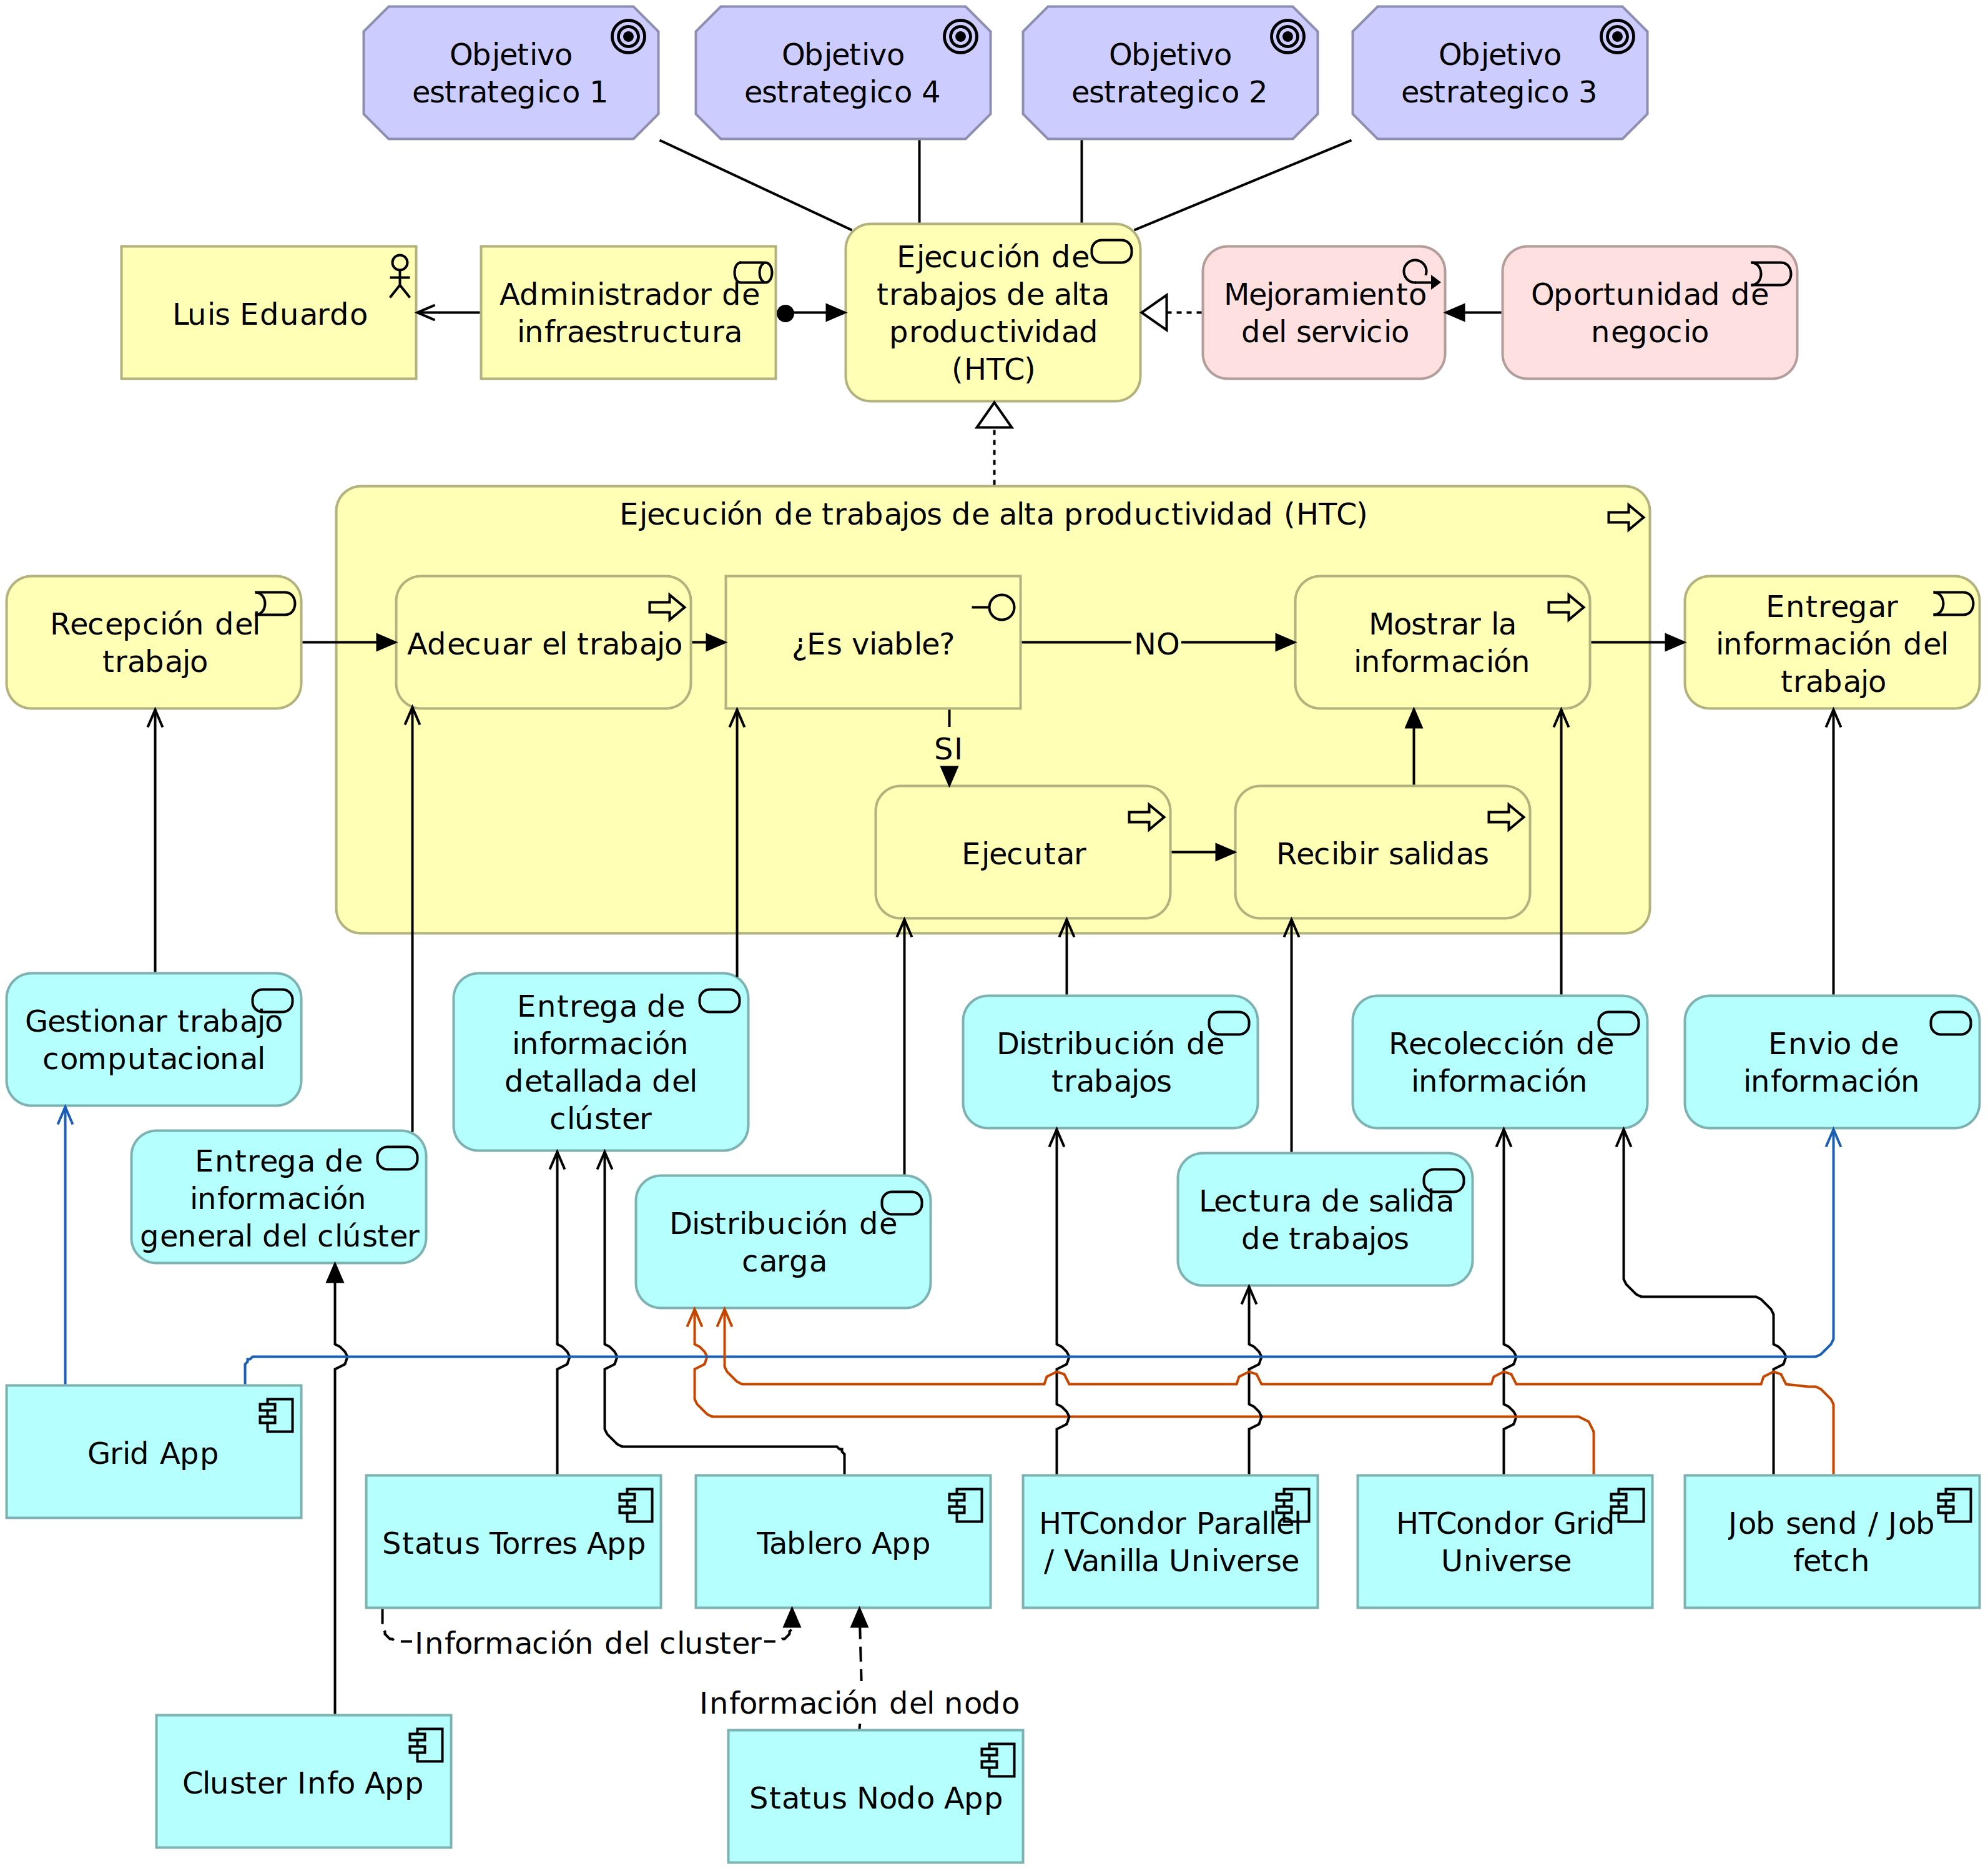
\includegraphics[scale=0.13]{tablas-images/archi/Business Service View.jpg}
	\caption{Vista de servicio de negocio}
    \label{fig:archiBSView}
\end{figure}

\subsection{Vista de aplicación}
\noindent
En la Figura \ref{fig:archiAppView} se muestran de forma general, las características y procesos de las aplicaciones que componen la solución, además de la comunicación entre dichas aplicaciones y la información de intercambio. Sin embargo, la vista que nos ofrece ArchiMate en capa de aplicación puede ser un poco limitada cuando el objetivo es describir a detalle la forma en que funciona cada componente de la aplicación y del sistema en general. Por lo que se decide complementar este modelo con otros diagramas usando otros lenguajes de modelado un poco más adelante.

\begin{figure}[H]
	\centering
	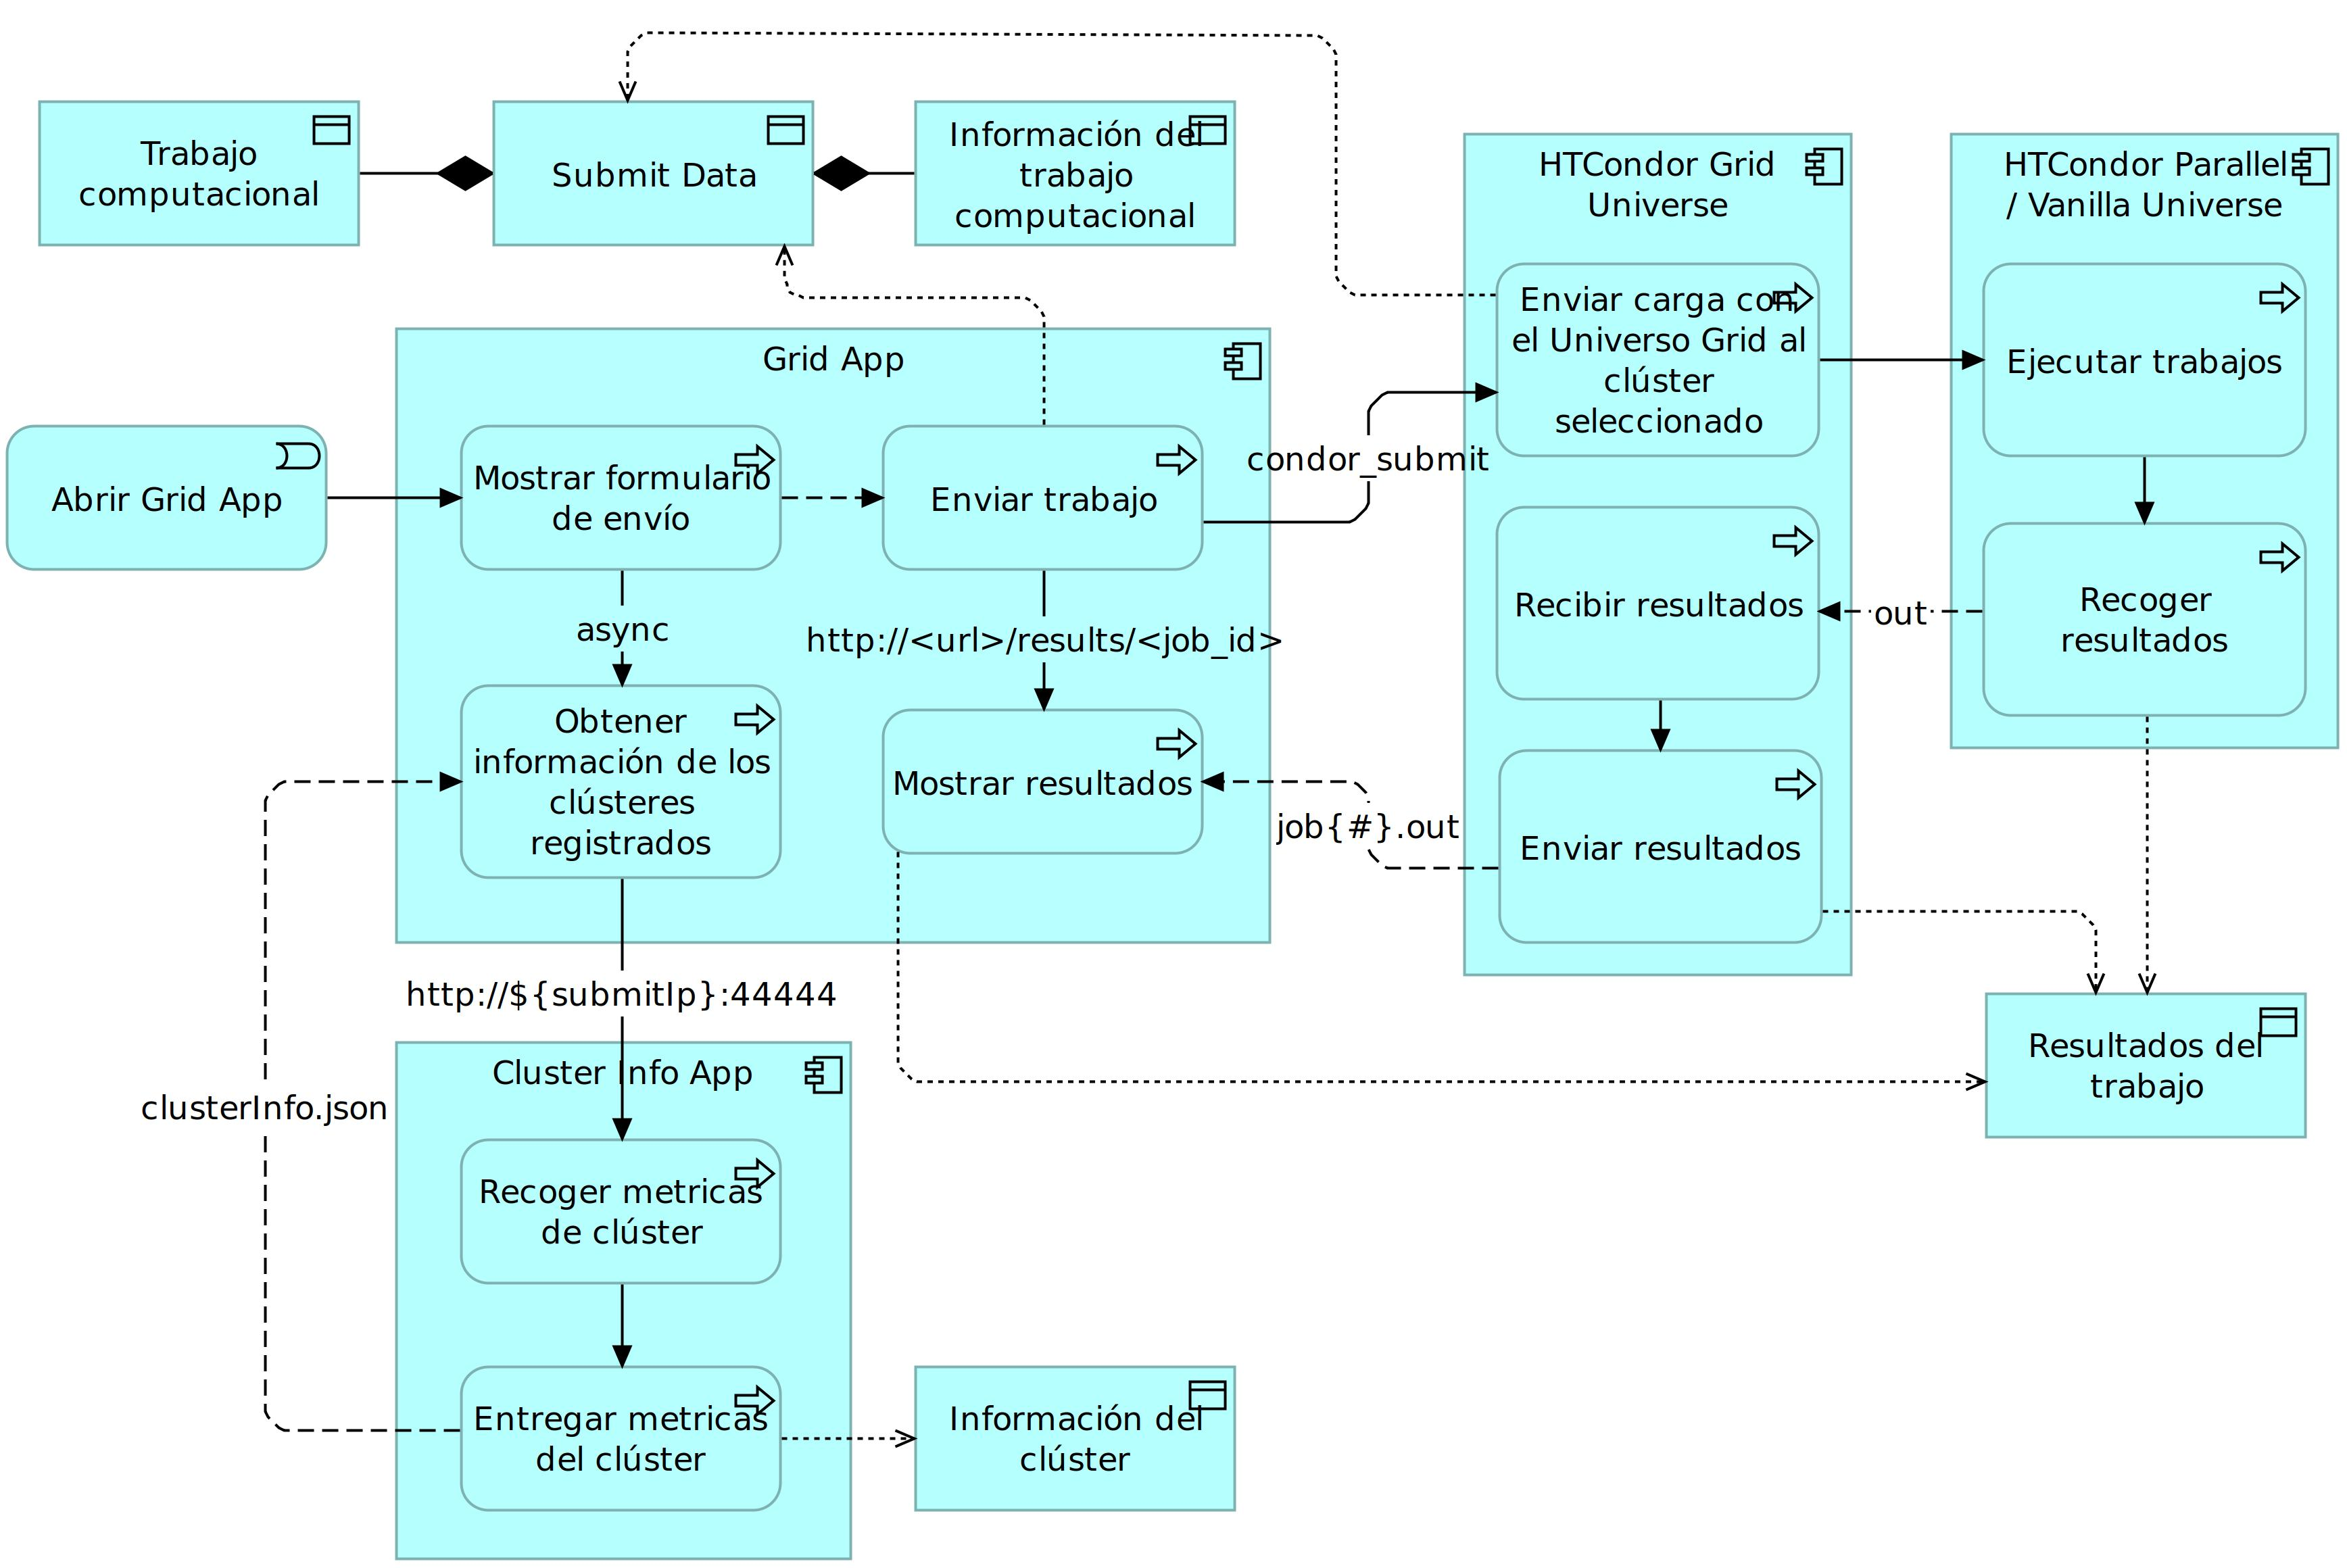
\includegraphics[scale=0.12]{tablas-images/archi/Application View.jpg}
	\caption{Vista de aplicación}
    \label{fig:archiAppView}
\end{figure}

\subsection{Vista de infraestructura}
\noindent
En la Figura \ref{fig:archiInfrastructureView} se muestran de forma general, las características de los nodos de la infraestructura que componen la solución, además de las relaciones entre dichos nodos y su relación con las aplicaciones que corren en ellos. Sin embargo, al igual que pasa en la capa de aplicación, la vista que nos ofrece ArchiMate en capa de infraestructura puede ser un poco limitada cuando el objetivo es describir a detalle la forma en que funciona cada nodo de la infraestructura y su comunicación física. Por lo que se decide complementar este modelo con otros diagramas usando otros lenguajes de modelado un poco más adelante.

\begin{figure}[H]
	\centering
	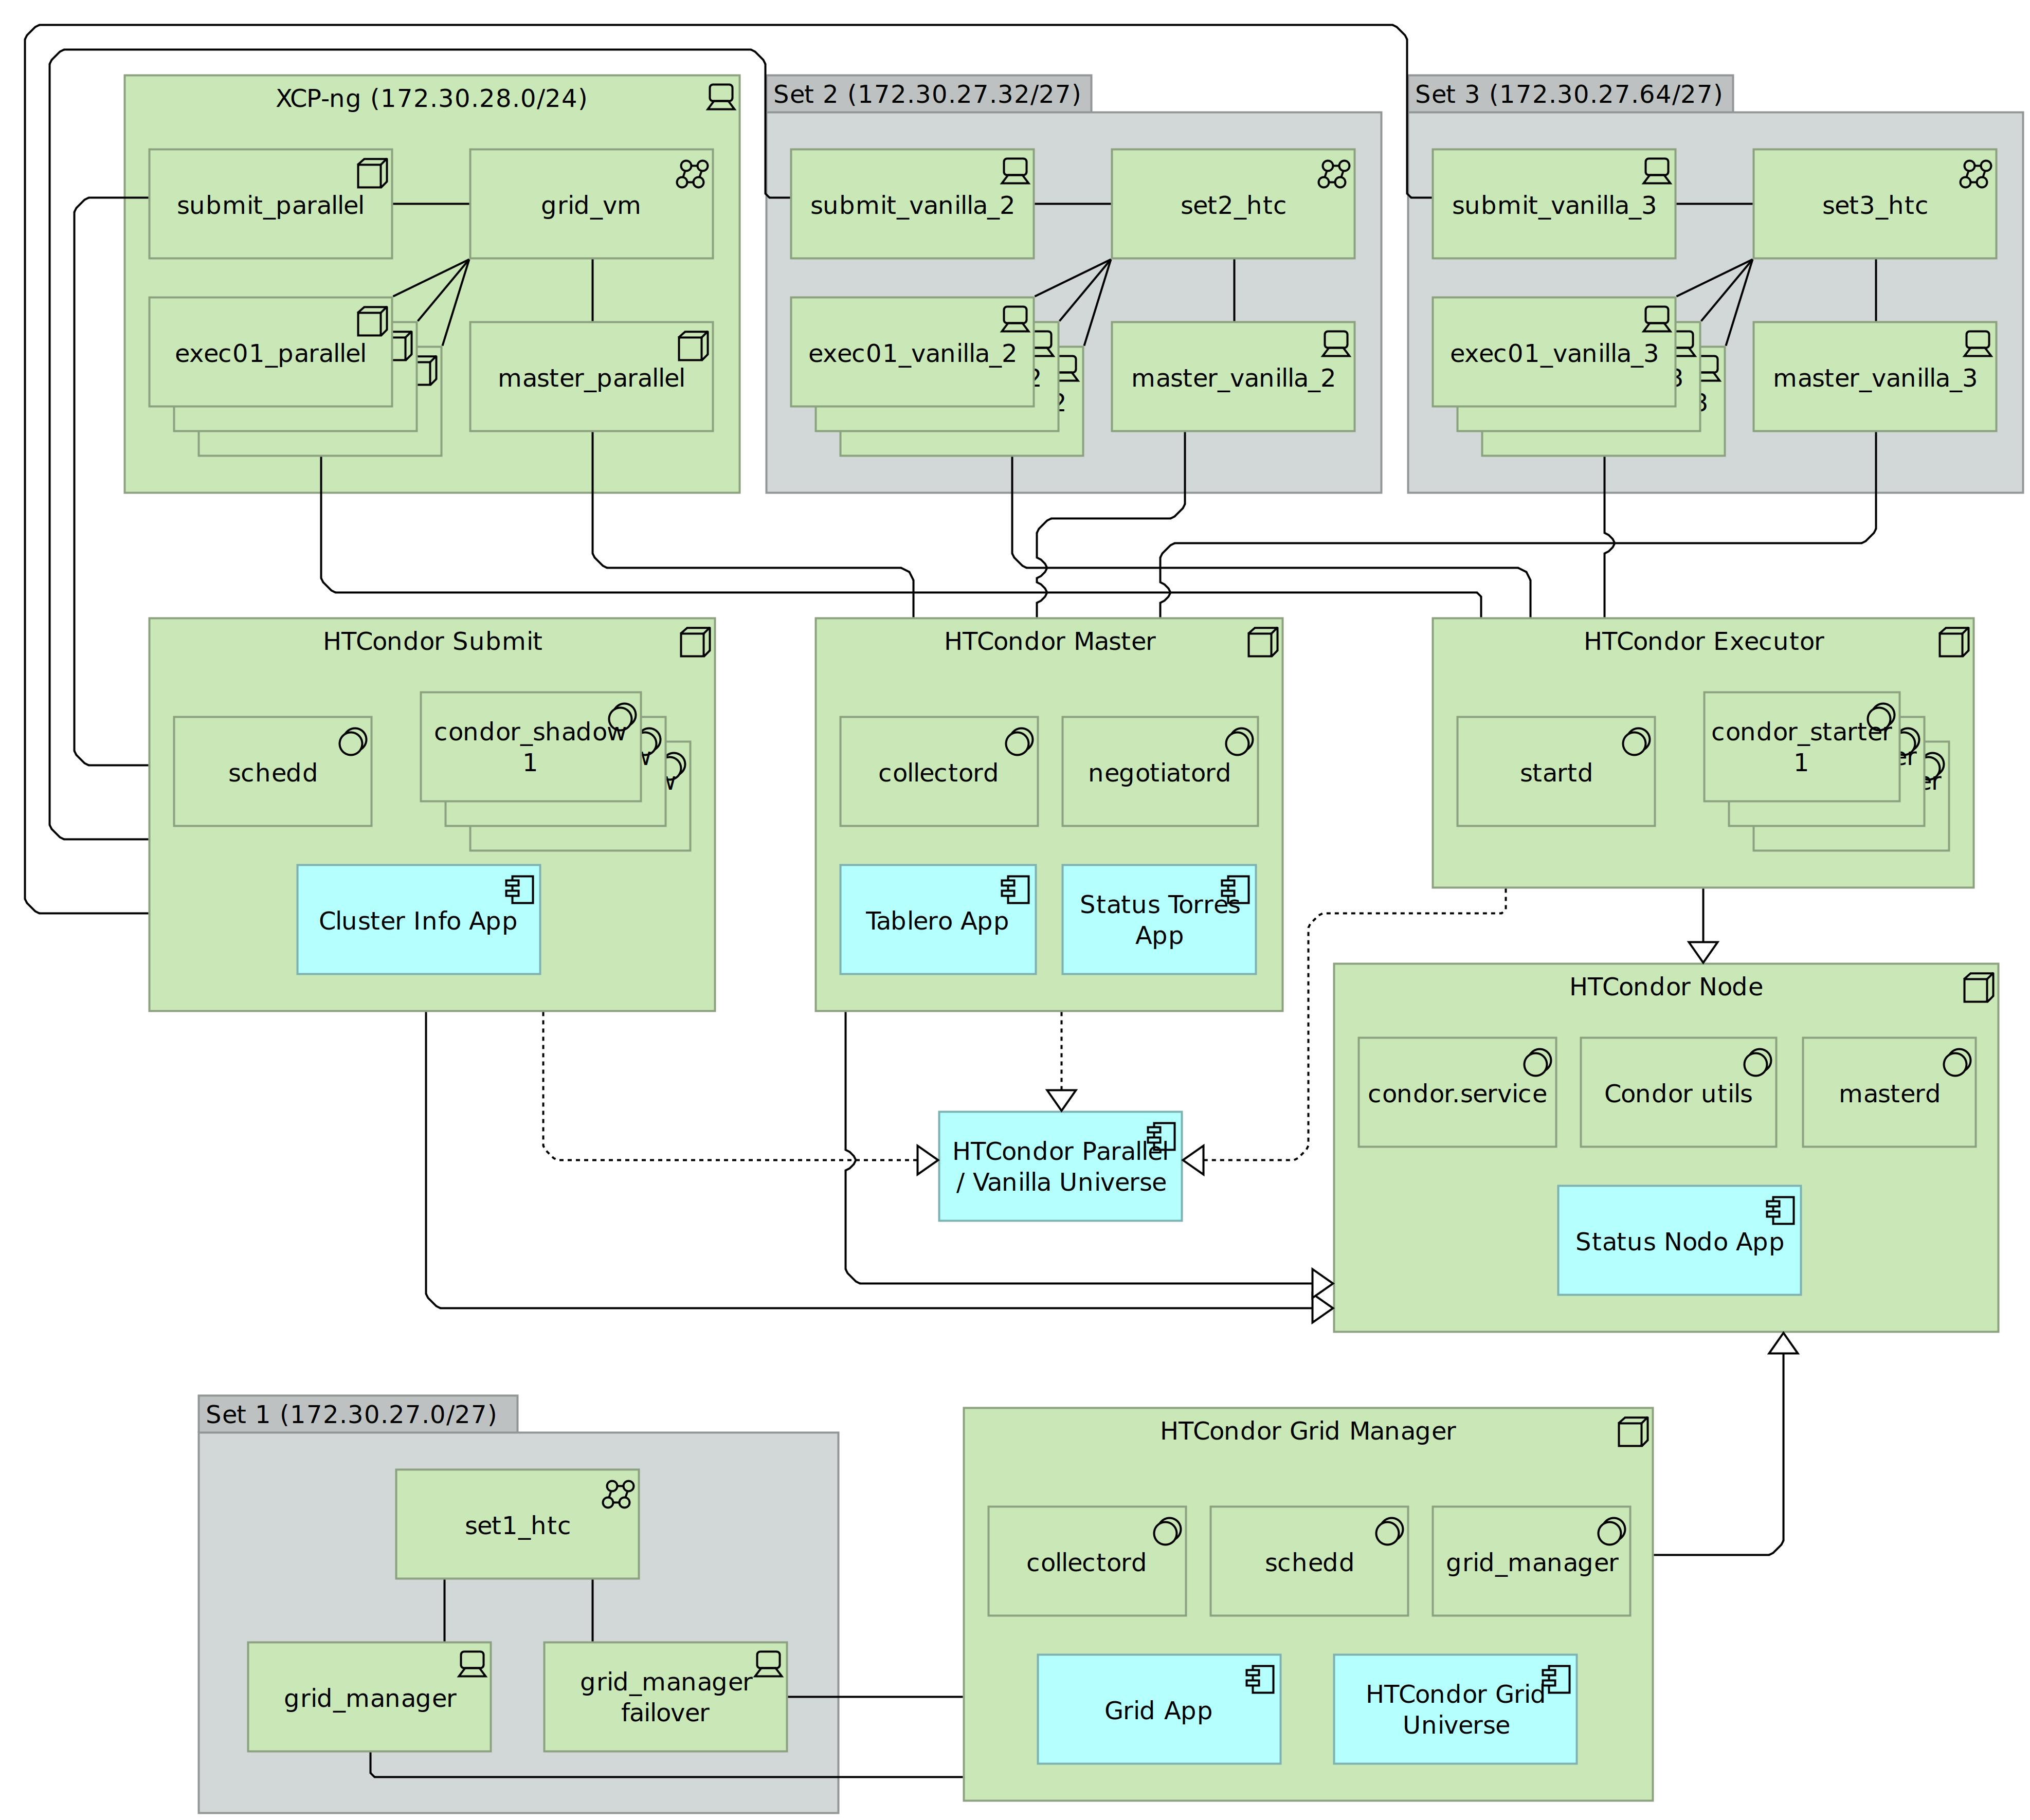
\includegraphics[scale=0.103]{tablas-images/archi/Infrastructure View.jpg}
	\caption{Vista de infraestructura}
    \label{fig:archiInfrastructureView}
\end{figure}

\subsection{Vista por capas}
\noindent
El último modelo de ArchiMate que compone la solución es el mostrado en la Figura \ref{fig:archiLayeredView} en donde se unen de forma general los demás modelos mostrados anteriormente y se muestran sus relaciones a alto nivel. Todo esto con el fin de dar una visión general de las capas que componen la solución y así tener una idea global de la forma en que cada componente se comunica con los demás.

\begin{figure}[H]
	\centering
	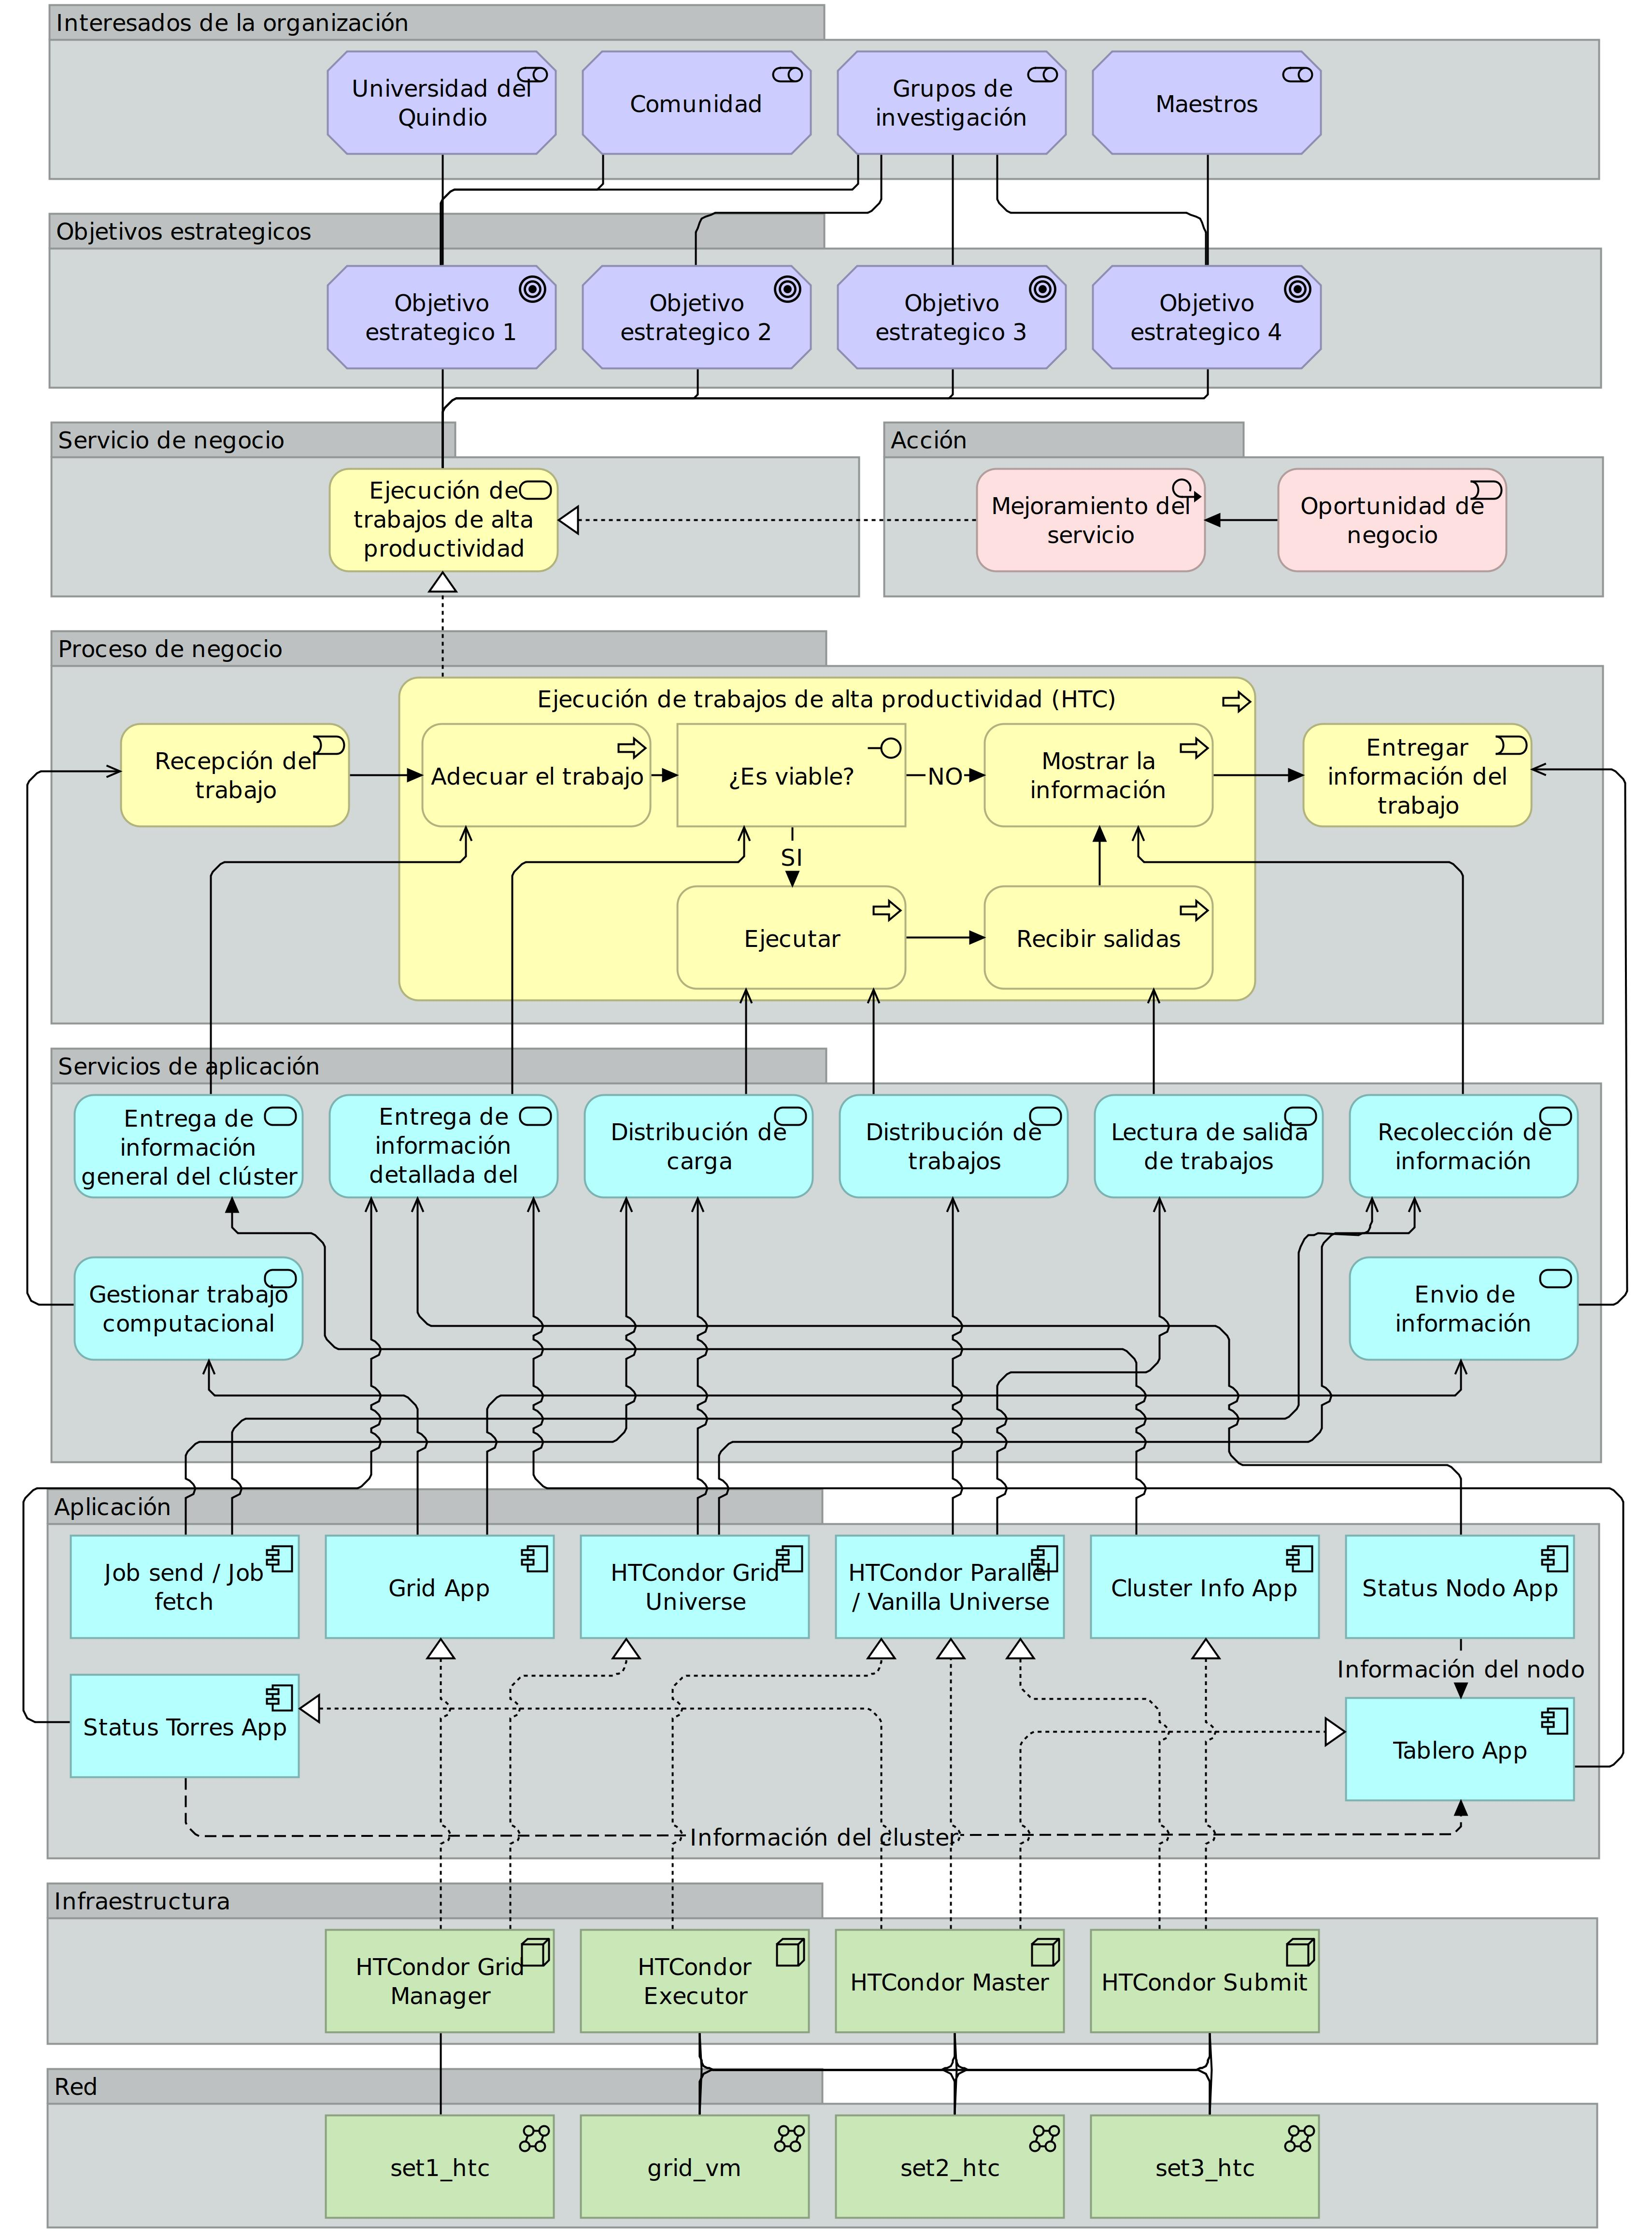
\includegraphics[scale=0.125]{tablas-images/archi/Layered View.jpg}
	\caption{Vista por capas}
    \label{fig:archiLayeredView}
\end{figure}

\section{Modelado del software con el modelo C4}
El modelo C4 es una herramienta que ayuda a los equipos de desarrollo de software a describir y comunicar la arquitectura del software a varios niveles de detalle. De forma general el modelo C4 tiene cuatro niveles, cada una con mayor nivel de detalle que la anterior. Para el caso de uso de este proyecto se optó por usar los tres primeros niveles, ya que se considera que el último nivel no da demasiado detalle visual para representar las interacciones en el ámbito de código, por lo que para este fin se usará otro diagrama presentado más adelante.

\subsection{Nivel 1: Diagrama de contexto del sistema}
\noindent
El diagrama de contexto del sistema muestra de forma muy general y a muy alto nivel la solución que se propone. Lo que permite una visión global y generalizada, útil para comprender rápidamente los elementos de la solución.

En la Figura \ref{fig:C4Nivel1} se muestra los elementos principales de la arquitectura, los nombres de dichos elementos, la interacción entre ellos y la comunicación que realizan con el usuario. Como se puede apreciar en el diagrama, el sistema está compuesto de tres aplicaciones y los tres Universos de \HTCondor que componen la solución. Cabe aclarar que la aplicación denominada "Tablero App" ya estaba implementada en un clúster antes del inicio de este proyecto. Sin embargo, se adiciona a la arquitectura de la solución, ya que se hizo un esfuerzo para adaptar está en todos los clústeres \textit{Vanilla} que componen la solución.

\begin{figure}[H]
	\centering
	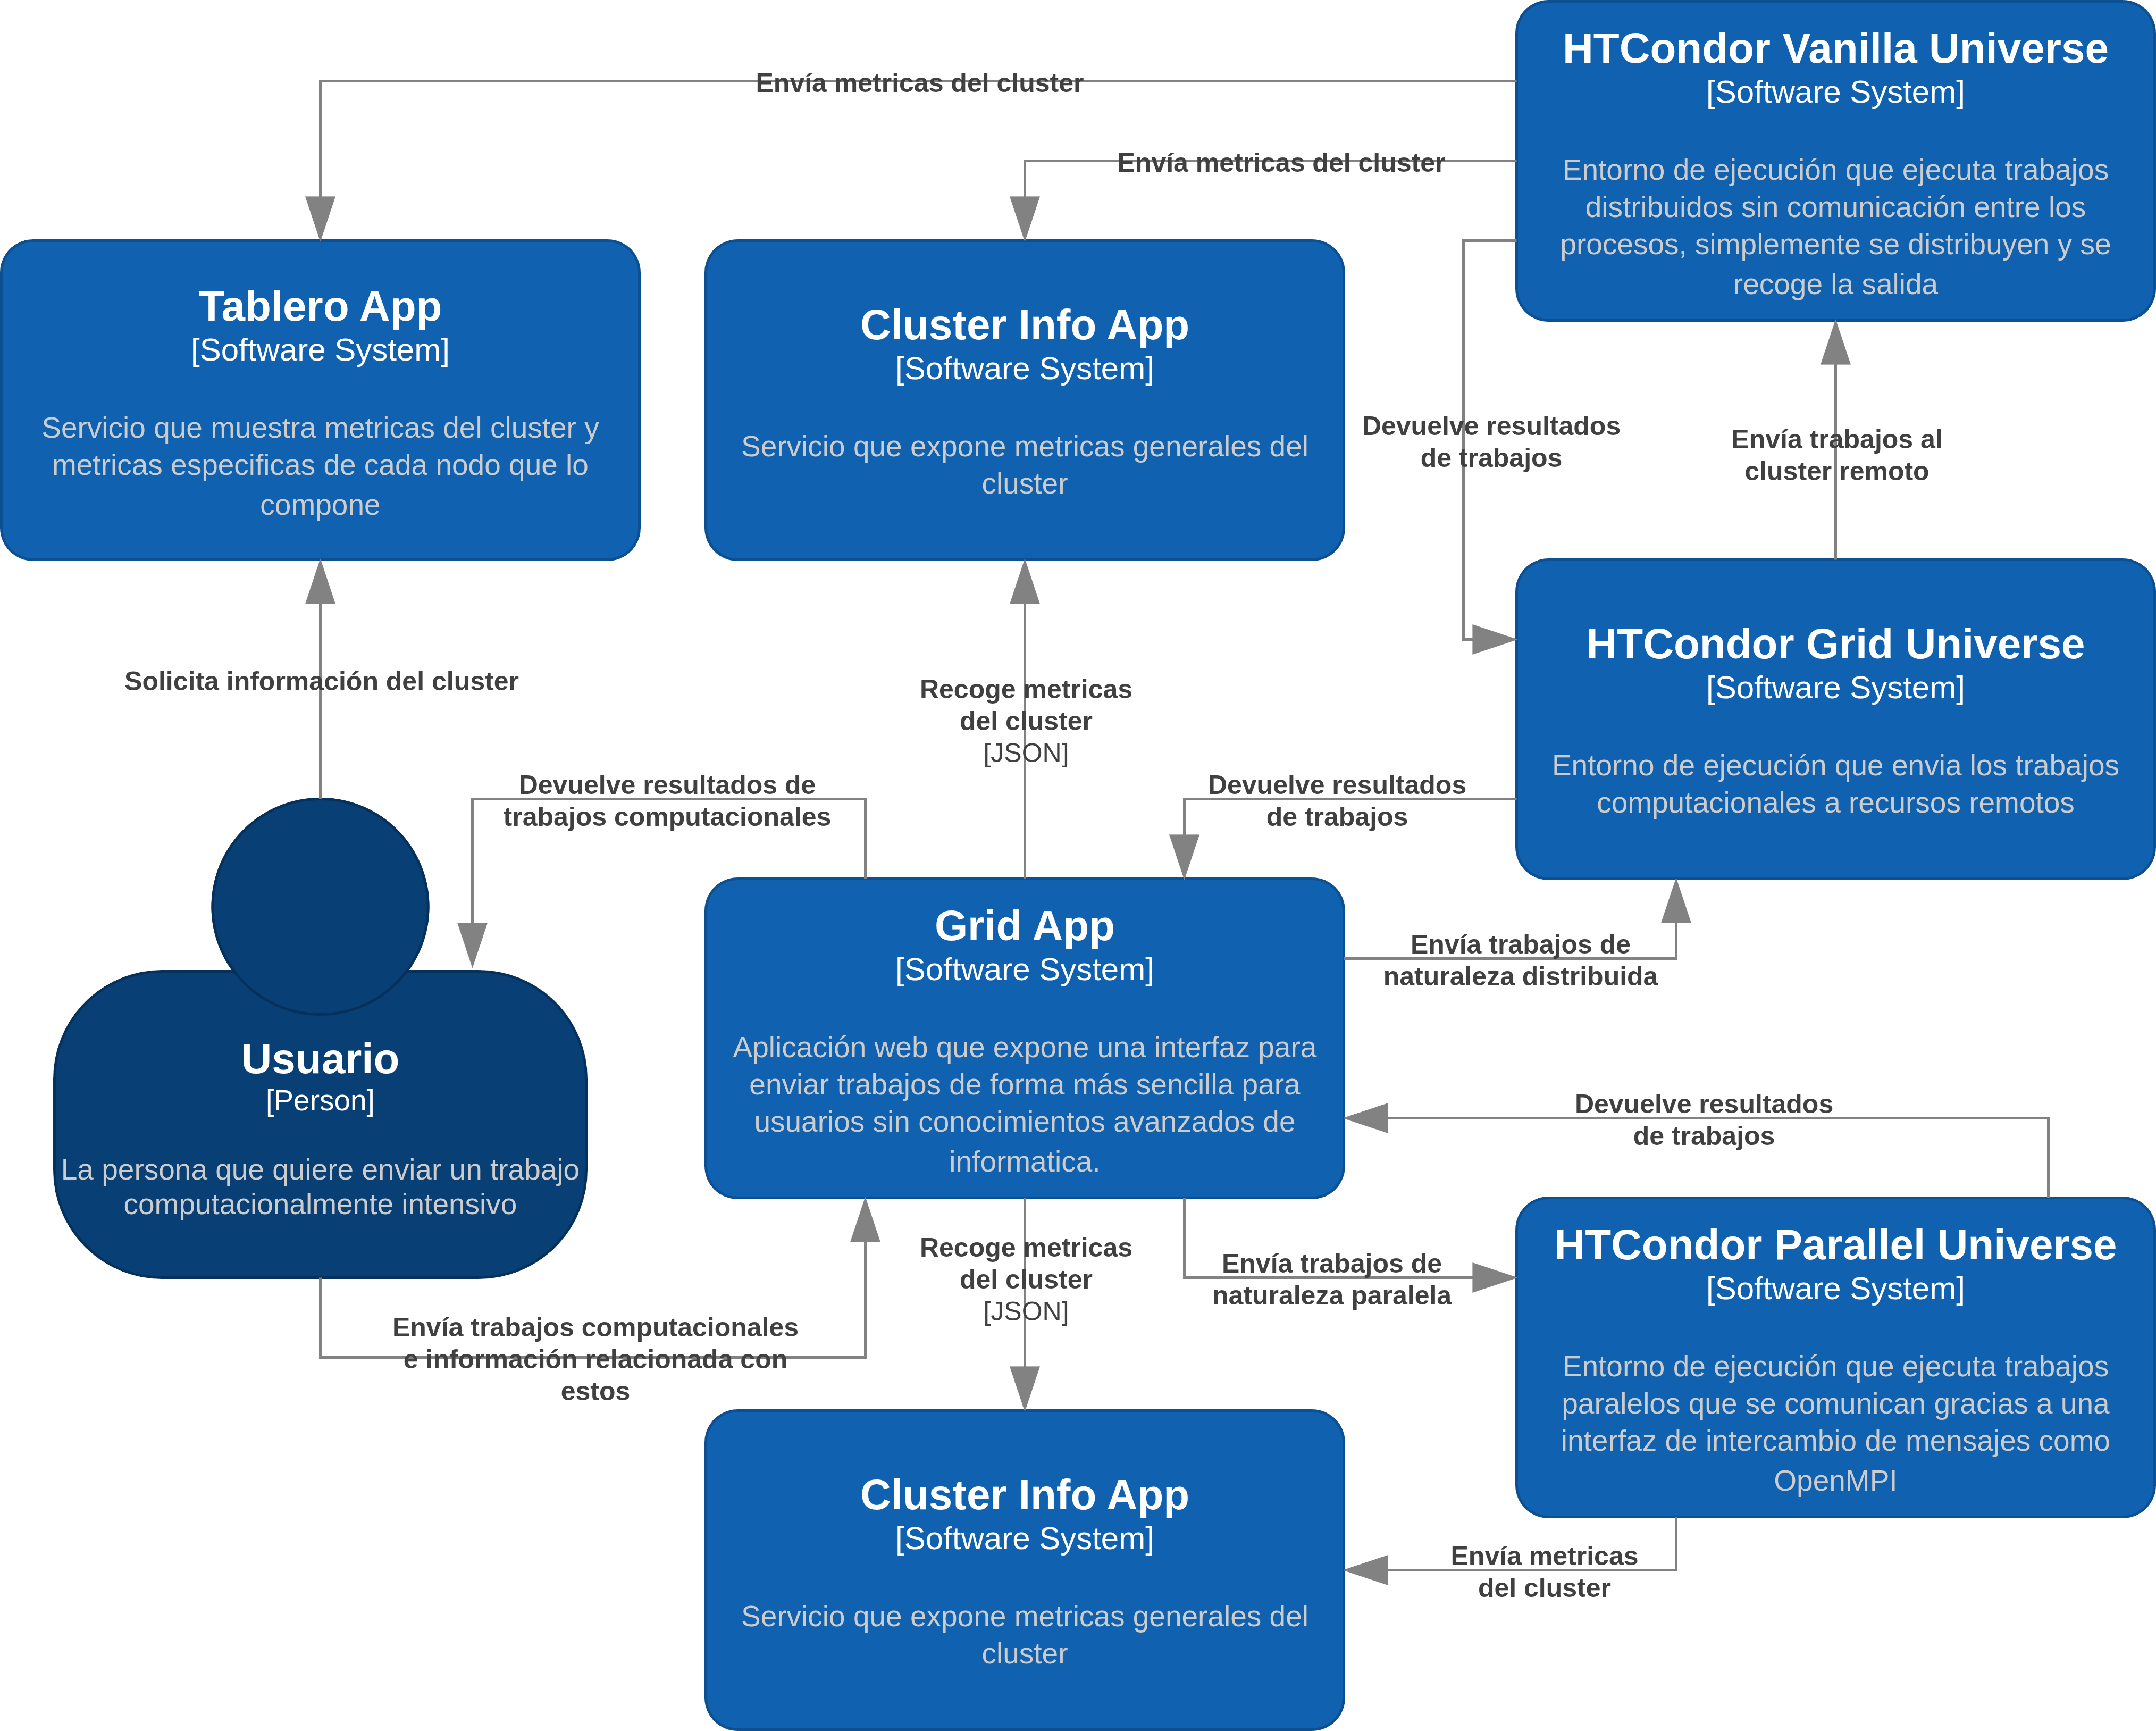
\includegraphics[scale=0.1]{tablas-images/C4/Diagramas HTCondor-Nivel 1.drawio.png}
	\caption{Diagrama de contexto del sistema}
    \label{fig:C4Nivel1}
\end{figure}

\subsection{Nivel 2: Diagrama de contenedores}
\noindent
El diagrama de contenedores muestra los elementos básicos dentro de cada sistema de Software. Lo que permite ir un poco más allá y entender como funciona cada sistema de software por dentro y como interactúa con el resto de contenedores.

En la Figura \ref{fig:C4Nivel2} se muestran los contenedores principales de la arquitectura, los nombres de dichos contenedores, la interacción entre ellos y la comunicación que realizan con el usuario. Como se puede apreciar en el diagrama, el sistema está compuesto por: (1) Un \textit{BackEnd} que cumple dos funciones principales; la primera es renderizar las plantillas que se le van a mostrar al usuario pues estás contienen información dinámica que debe ser consultada y establecida por el servidor, la segunda es realizar toda la lógica de la aplicación como despertar otros procesos o construir los archivos maestros de \HTCondor. Se optó por este enfoque en el diseño para propender por la simplicidad de la aplicación y su fácil portabilidad y despliegue en diferentes tipos de entornos. En el Apéndice XX se muestra el código de los componentes y la estructura de los directorios de este componente. (2) Un directorio dentro del sistema de archivos del equipo que sirve la aplicación \textit{Grid App} en donde se almacenan los resultados de los trabajos. (3) Los Universos de \HTCondor que se propusieron implementar en este proyecto, estos son, \textit{Parallel y Grid}, pues el \textit{Vanilla} ya estaba implementado y (4) una aplicación llamada \textit{Cluster Info App} en cada Clúster de \HTCondor que recoge métricas básicas y las expone en formato \JSON a través de una \API.

\begin{figure}[H]
	\centering
	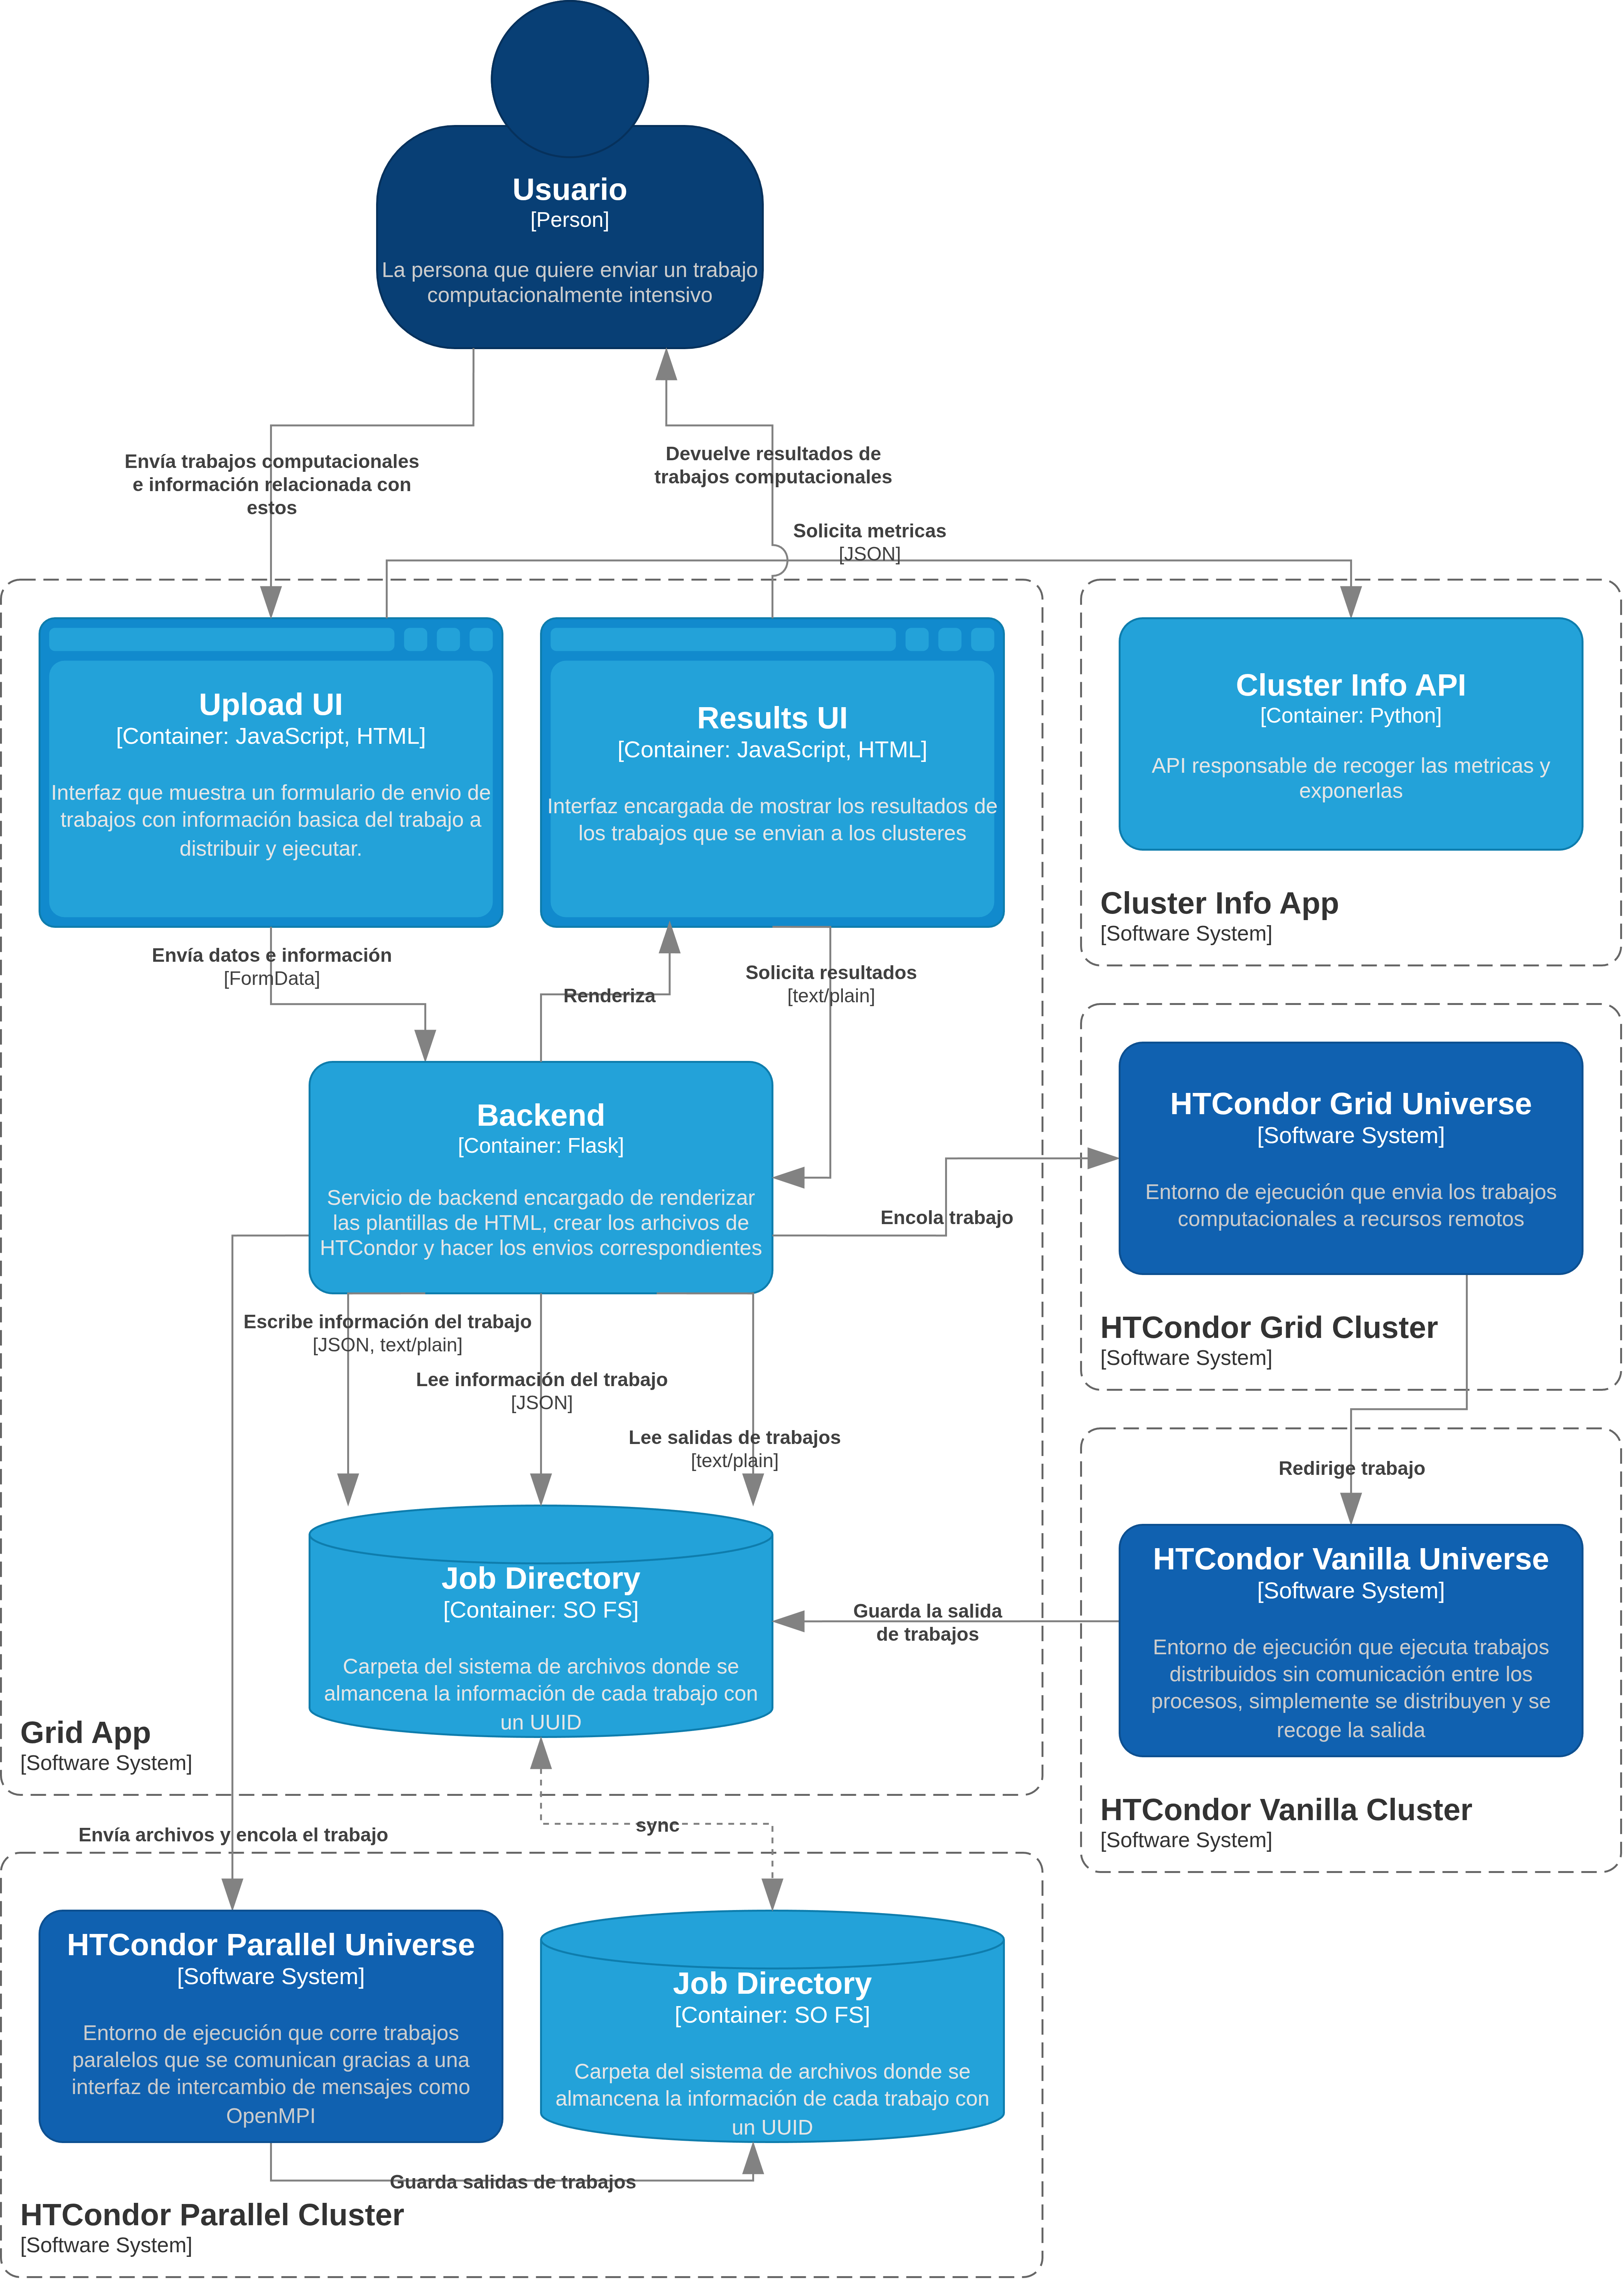
\includegraphics[scale=0.1]{tablas-images/C4/Diagramas HTCondor-Nivel 2.drawio.png}
	\caption{Diagrama de contenedores}
    \label{fig:C4Nivel2}
\end{figure}

\subsection{Nivel 3: Diagrama de componentes}
\noindent
El diagrama de componentes muestra los elementos básicos dentro de cada contenedor. Lo que permite ir aún más allá y entender de forma profunda como están compuestos los elementos del Software y que realizan a nivel interno. Para este nivel de granularidad se decide dividir el diagrama de componentes en distintas partes. Con el fin de hacer más sencilla su lectura y comprensión.

\subsubsection{Universo \textit{Vanilla}}
\noindent
En la Figura \ref{fig:C4Nivel3Vanilla} se muestran los componentes principales de la arquitectura del Universo \textit{Vanilla} en \HTCondor. Además, se pueden apreciar los distintos procesos que sigue un trabajo desde su envío hasta la recepción de sus resultados.

\begin{figure}[H]
	\centering
	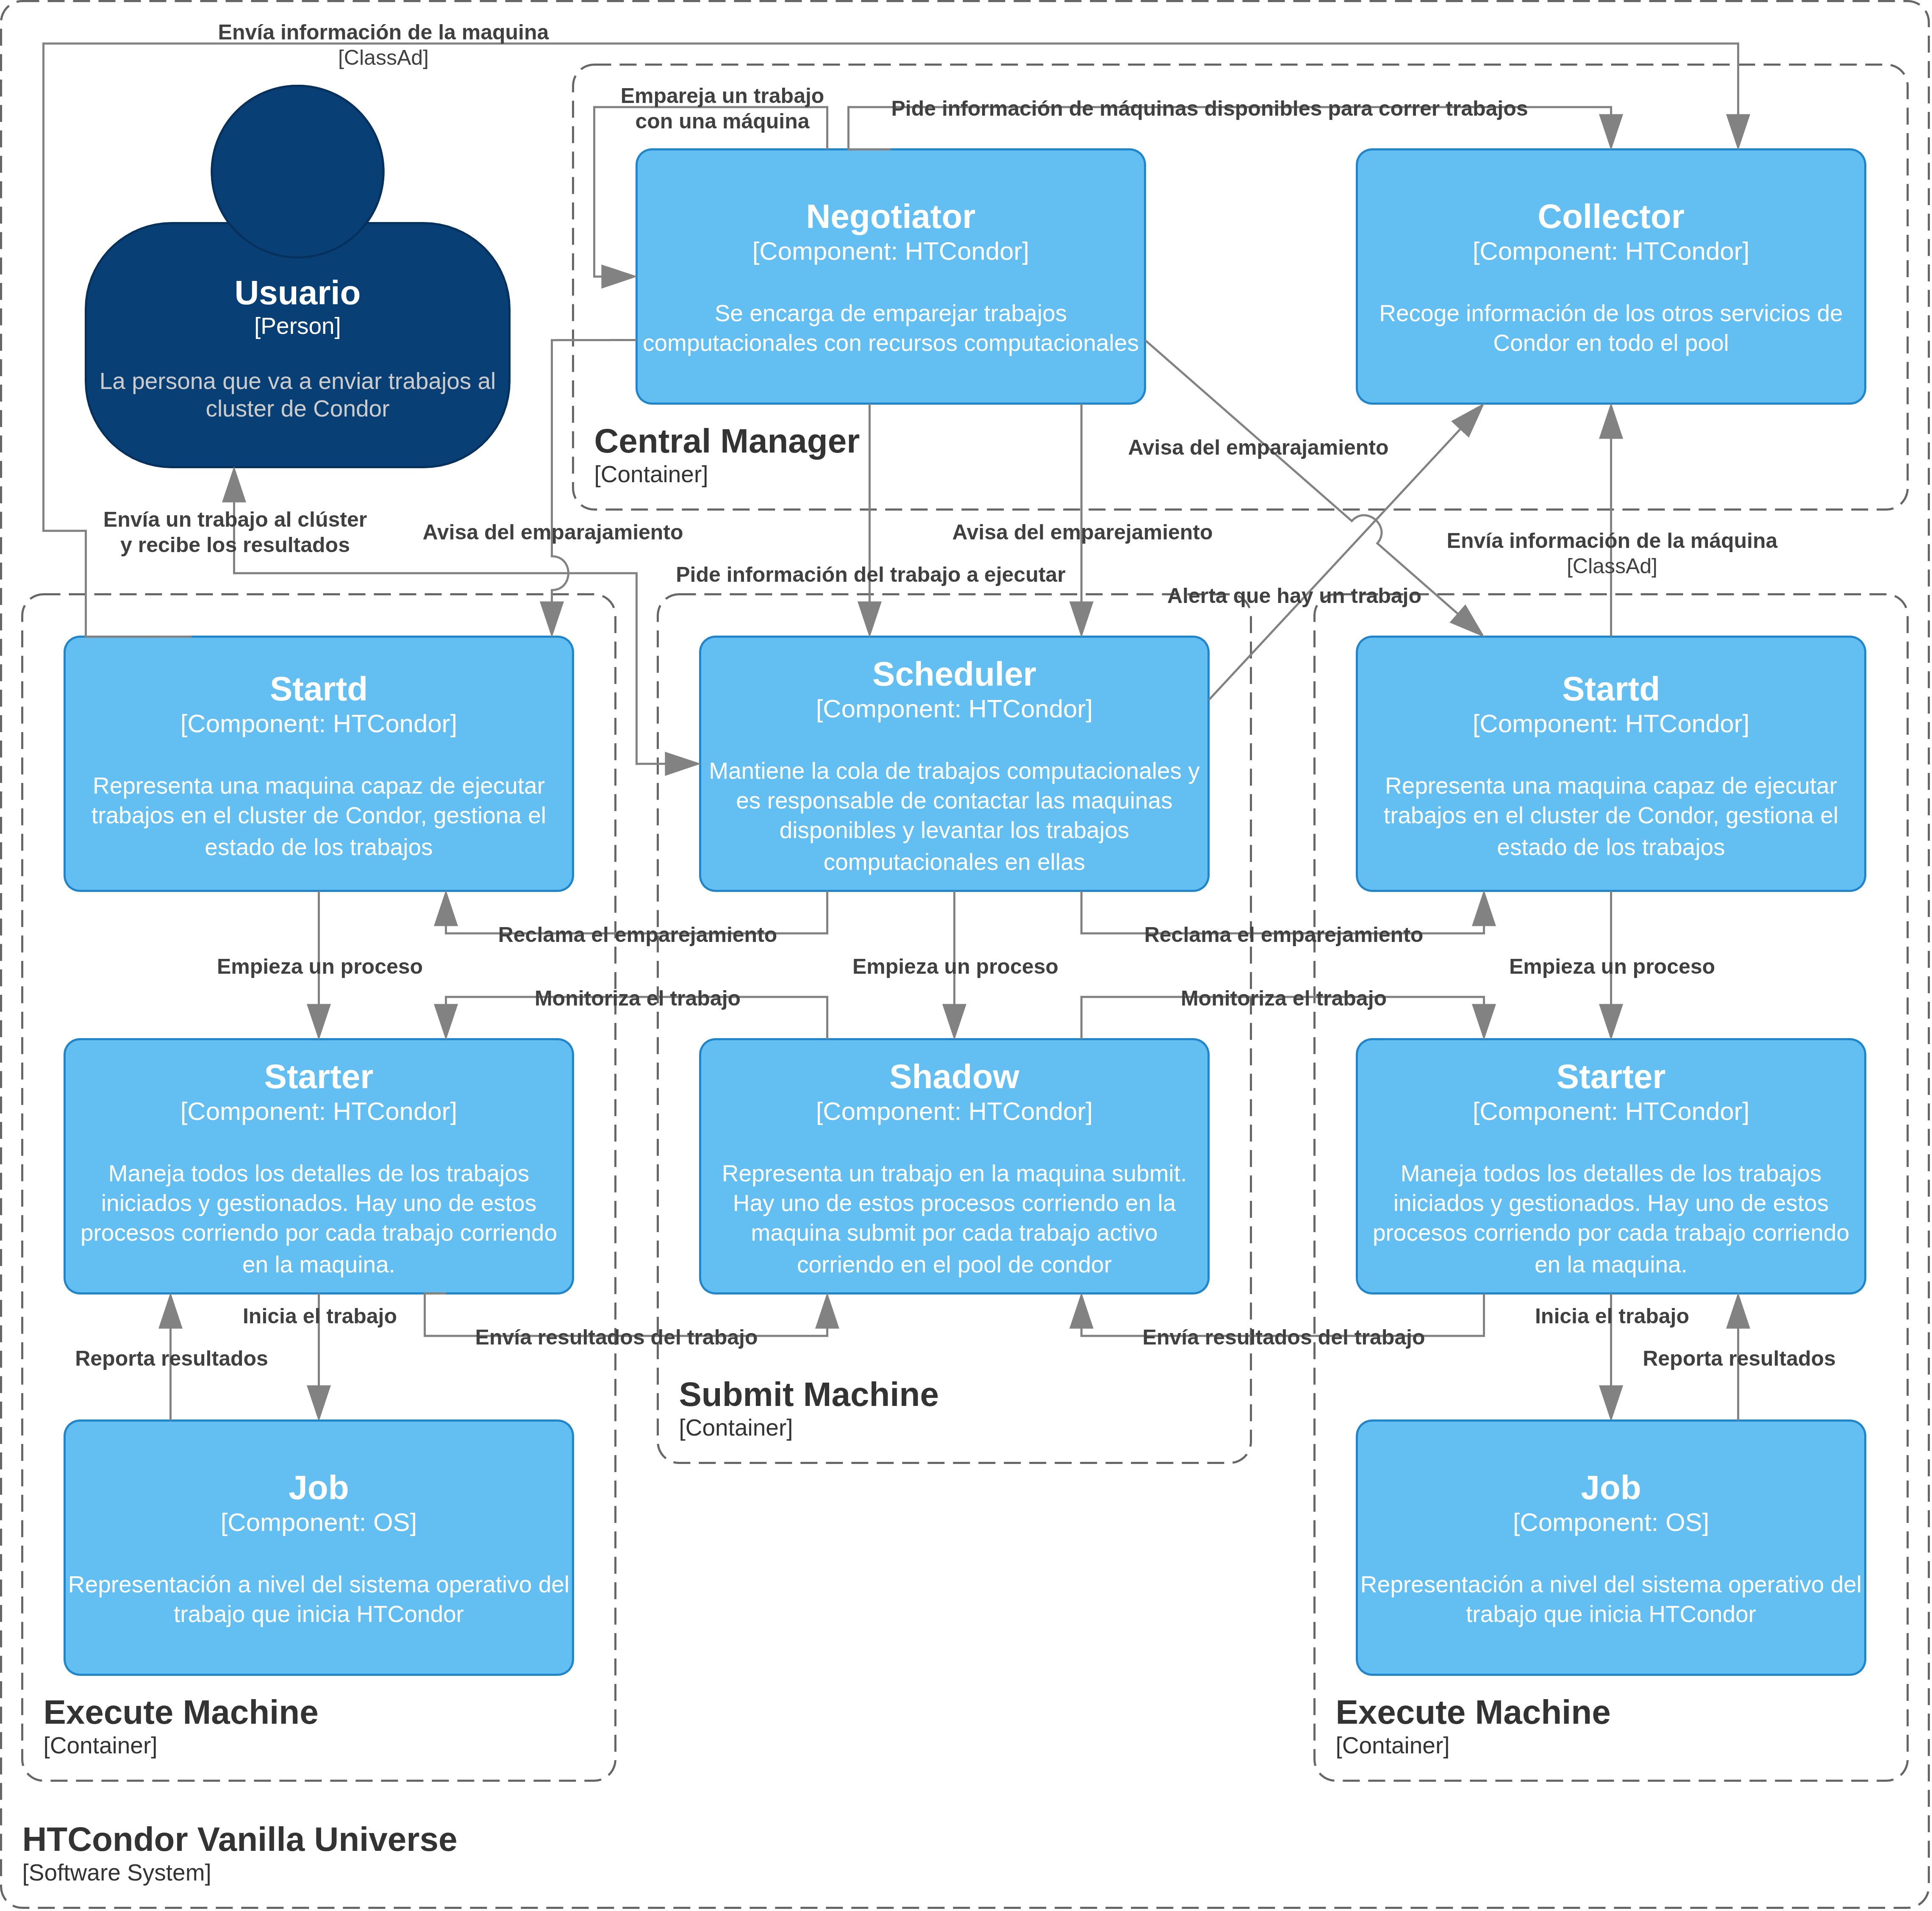
\includegraphics[scale=0.09]{tablas-images/C4/Diagramas HTCondor-Nivel 3 - Vanilla.drawio.png}
	\caption{Diagrama de componentes para el Universo \textit{Vanilla}}
    \label{fig:C4Nivel3Vanilla}
\end{figure}

\subsubsection{Universo \textit{Parallel}}
\noindent
En la Figura \ref{fig:C4Nivel3Parallel} se muestran los componentes principales de la arquitectura del Universo \textit{Parallel} en \HTCondor. Además, se pueden apreciar los distintos procesos que sigue un trabajo desde su envío hasta la recepción de sus resultados. Es importante notar que ls comunicación y los componentes funcionan exactamente de la misma forma que en el Universo \textit{Vanilla}, con la unica diferencia que aquí, los trabajo se comunican a través de \MPI.

\begin{figure}[H]
	\centering
	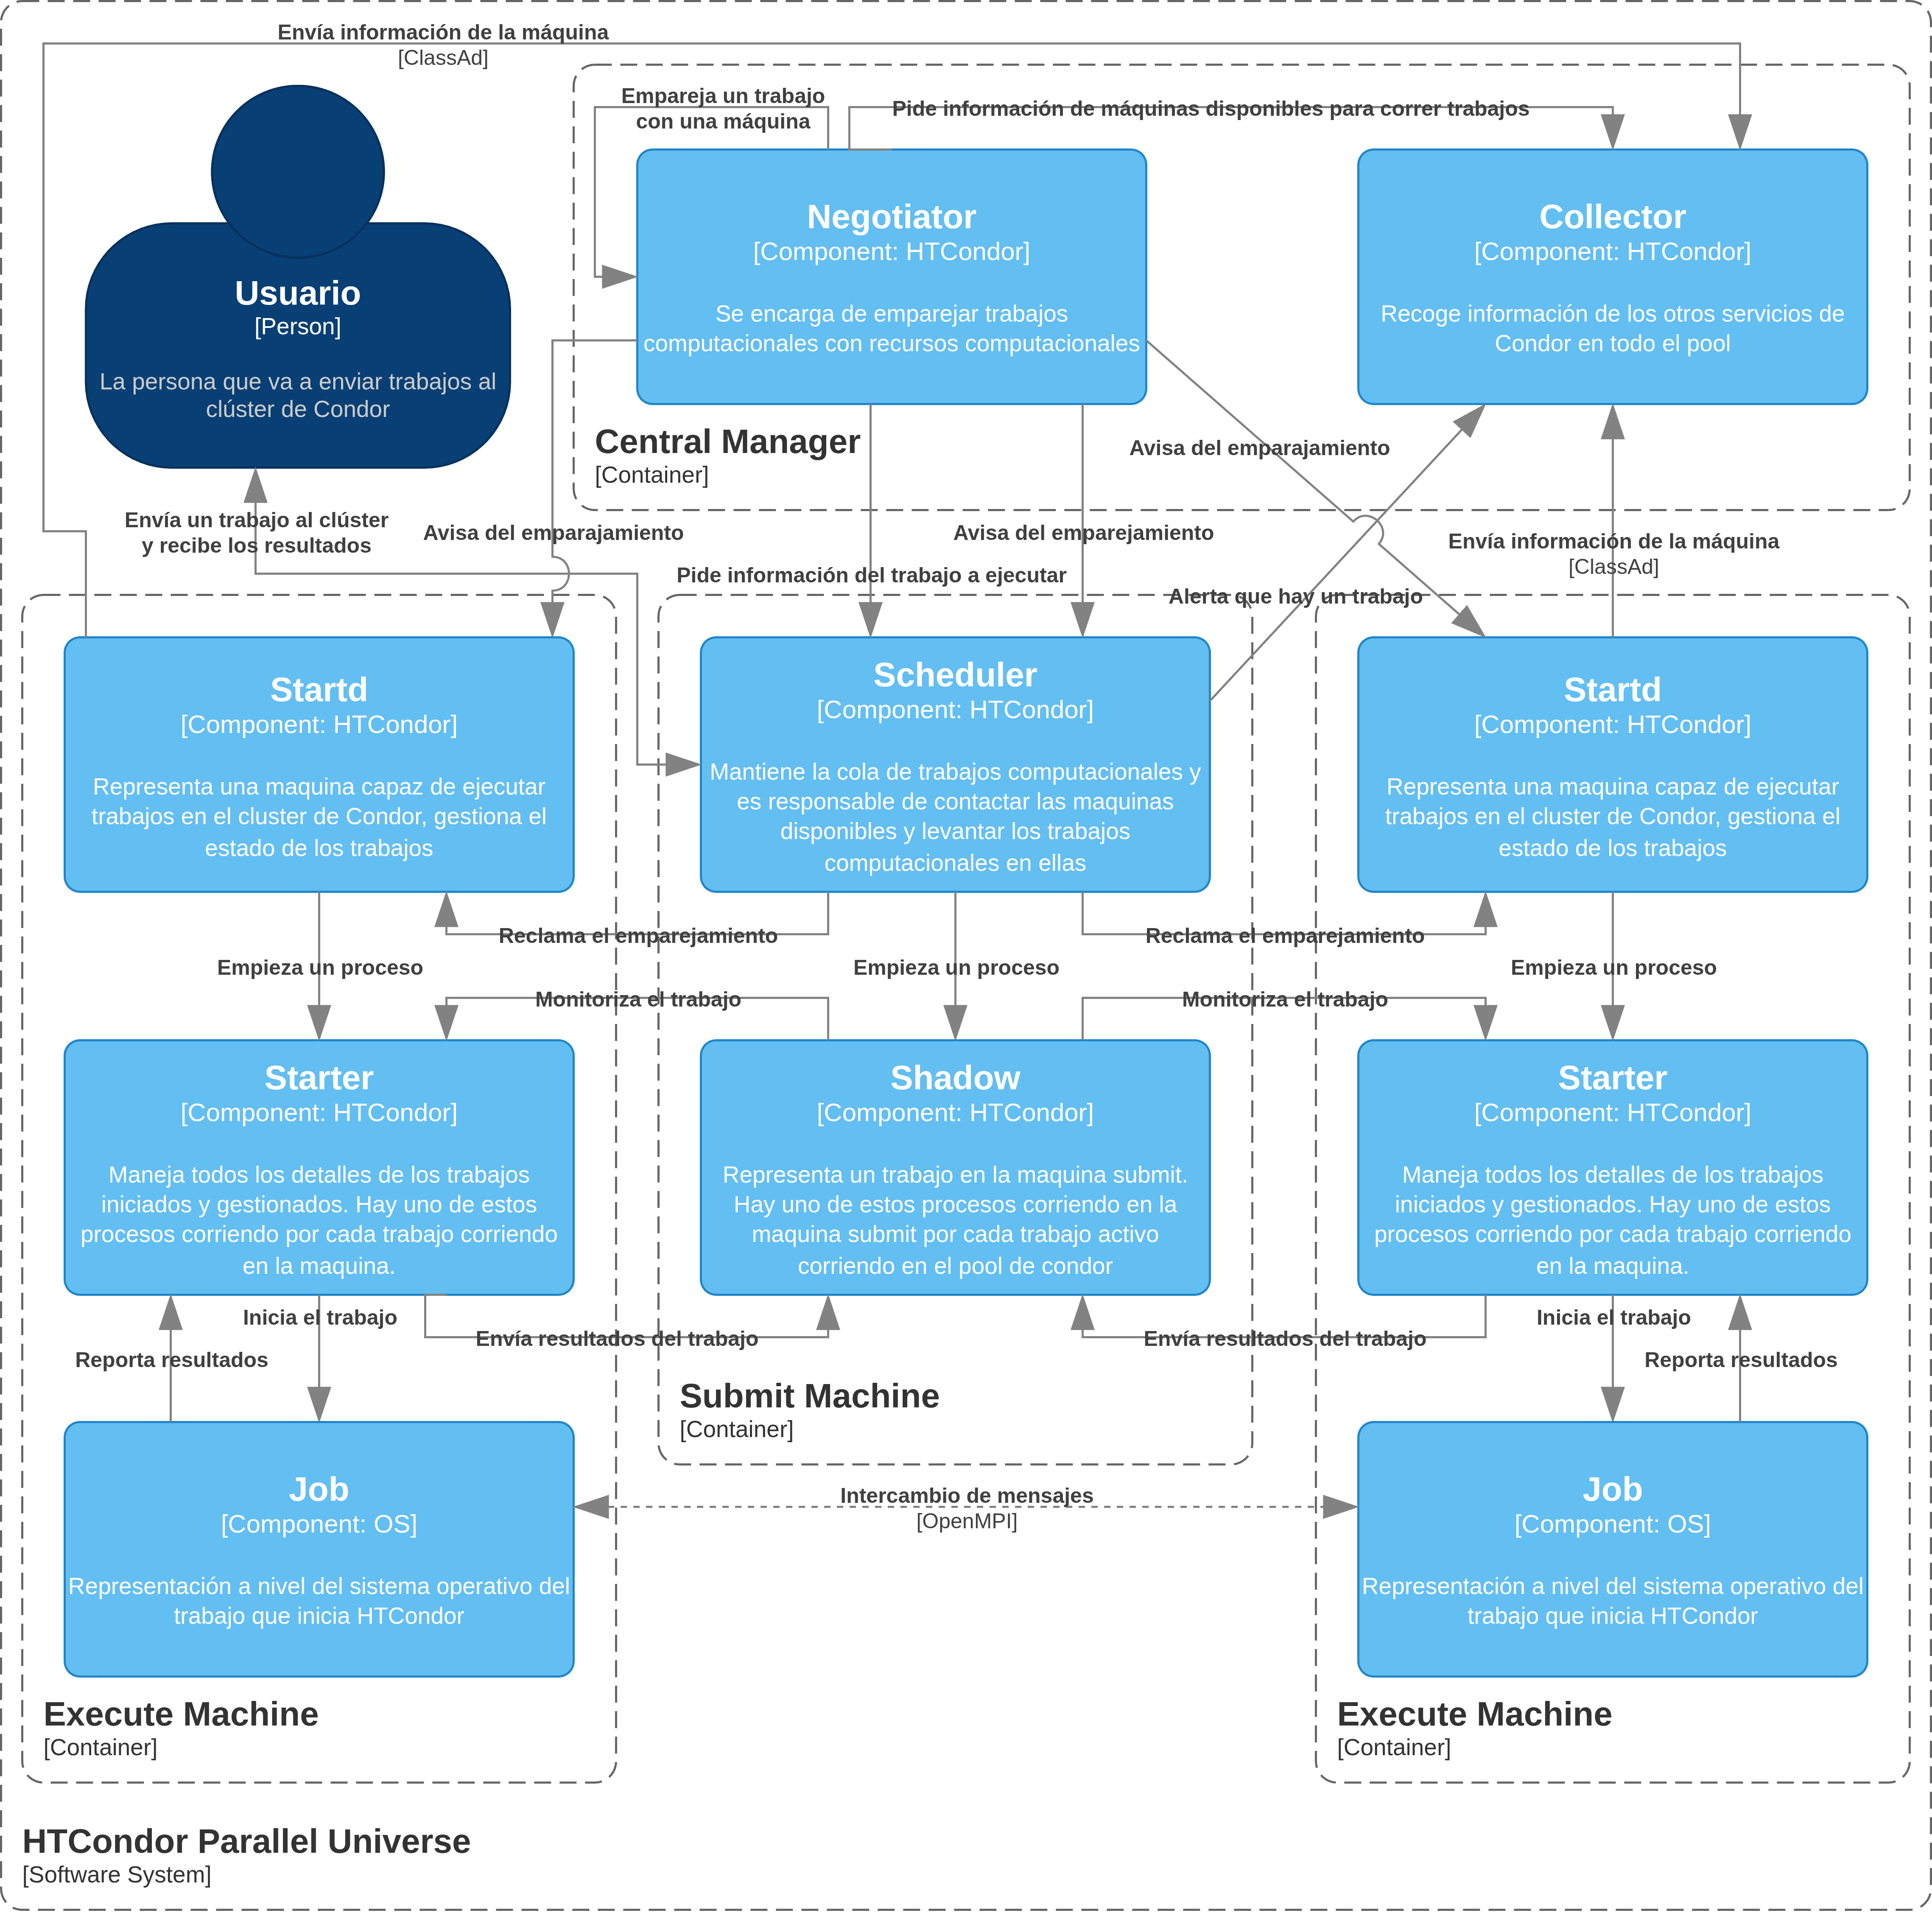
\includegraphics[scale=0.09]{tablas-images/C4/Diagramas HTCondor-Nivel 3 - Parallel.drawio.png}
	\caption{Diagrama de componentes para el Universo \textit{Parallel}}
    \label{fig:C4Nivel3Parallel}
\end{figure}

\subsubsection{Universo \textit{Grid}}
\noindent
En la Figura \ref{fig:C4Nivel3Grid} se muestran los componentes principales de la arquitectura del Universo \textit{Grid} en \HTCondor. Como se puede apreciar en el digrama este Universo actua como un intermediario entre el usuario y el clúster que va a ejecutar su trabajo, permitiendo así interconectar multiples clústeres, donde reside el valor de este Universo.

\begin{figure}[H]
	\centering
	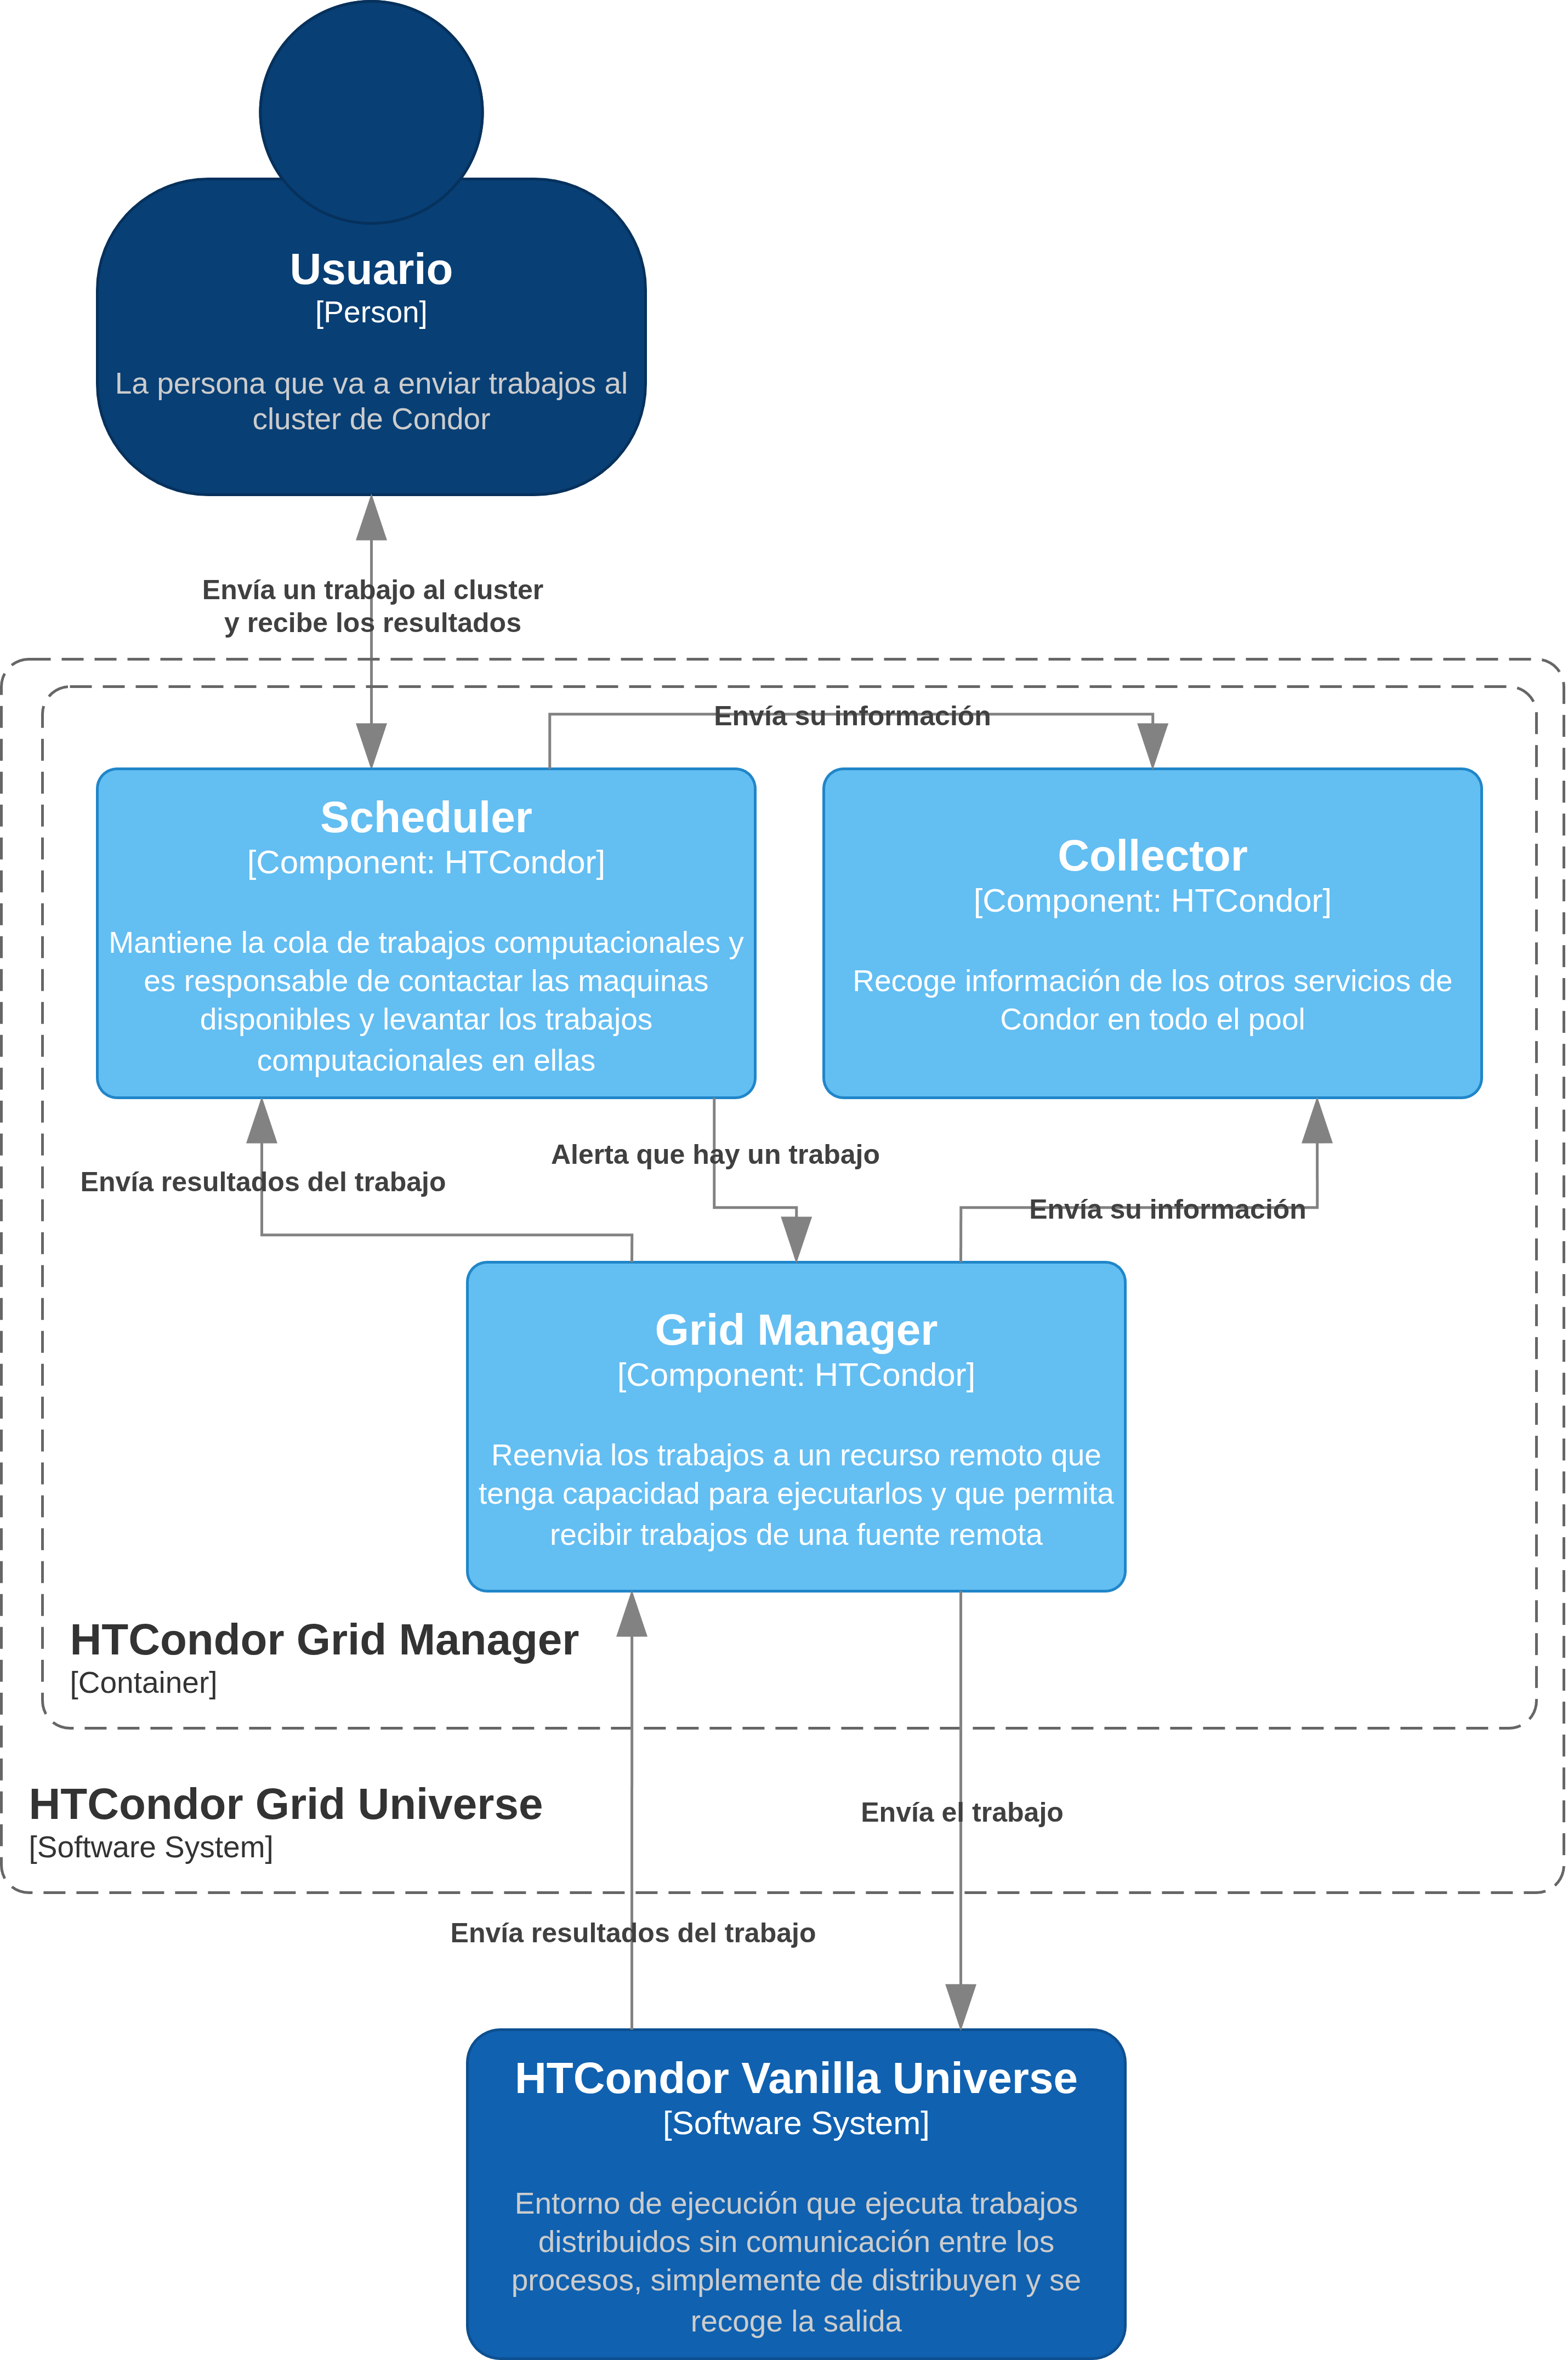
\includegraphics[scale=0.1]{tablas-images/C4/Diagramas HTCondor-Nivel 3 - Grid.drawio.png}
	\caption{Diagrama de componentes para el Universo \textit{Grid}}
    \label{fig:C4Nivel3Grid}
\end{figure}

\subsubsection{Aplicaciones de Software}
\noindent
En la Figura \ref{fig:C4Nivel3Apps} se muestran los componentes principales de las aplicaciones que integran el sistema. Como se puede evidenciar en el diagrama, hay dos aplicaciones principales que conforman este sistema. La primera es la aplicación central \textit{Grid App} que ayuda a abstraer la complejidad de \HTCondor con una interfaz Web más amigable, además, es la encargada de enviar los trabajos y recoger los resultados. La segunda es \textit{Cluster Info App} que ayuda a exponer métricas de cada clúster, permitiendo así a la aplicación central obtener datos reales de cada clúster y permitir al usuario elegir el clúster con métricas más favorables para su caso de uso. Es importante aclarar que la aplicación \textit{Tablero App} también está disponible y funcionando en algunos de los clústeres que componen la solución. Sin embargo, dado que su única labor es mostrar métricas detalladas del clúster, se opta por no agregarlo al diagrama por dos razones: (1) para reducir su complejidad y (2) porque el desarrollo de esta aplicación no es resultado del desarrollo de este proyecto.

\begin{figure}[H]
	\centering
	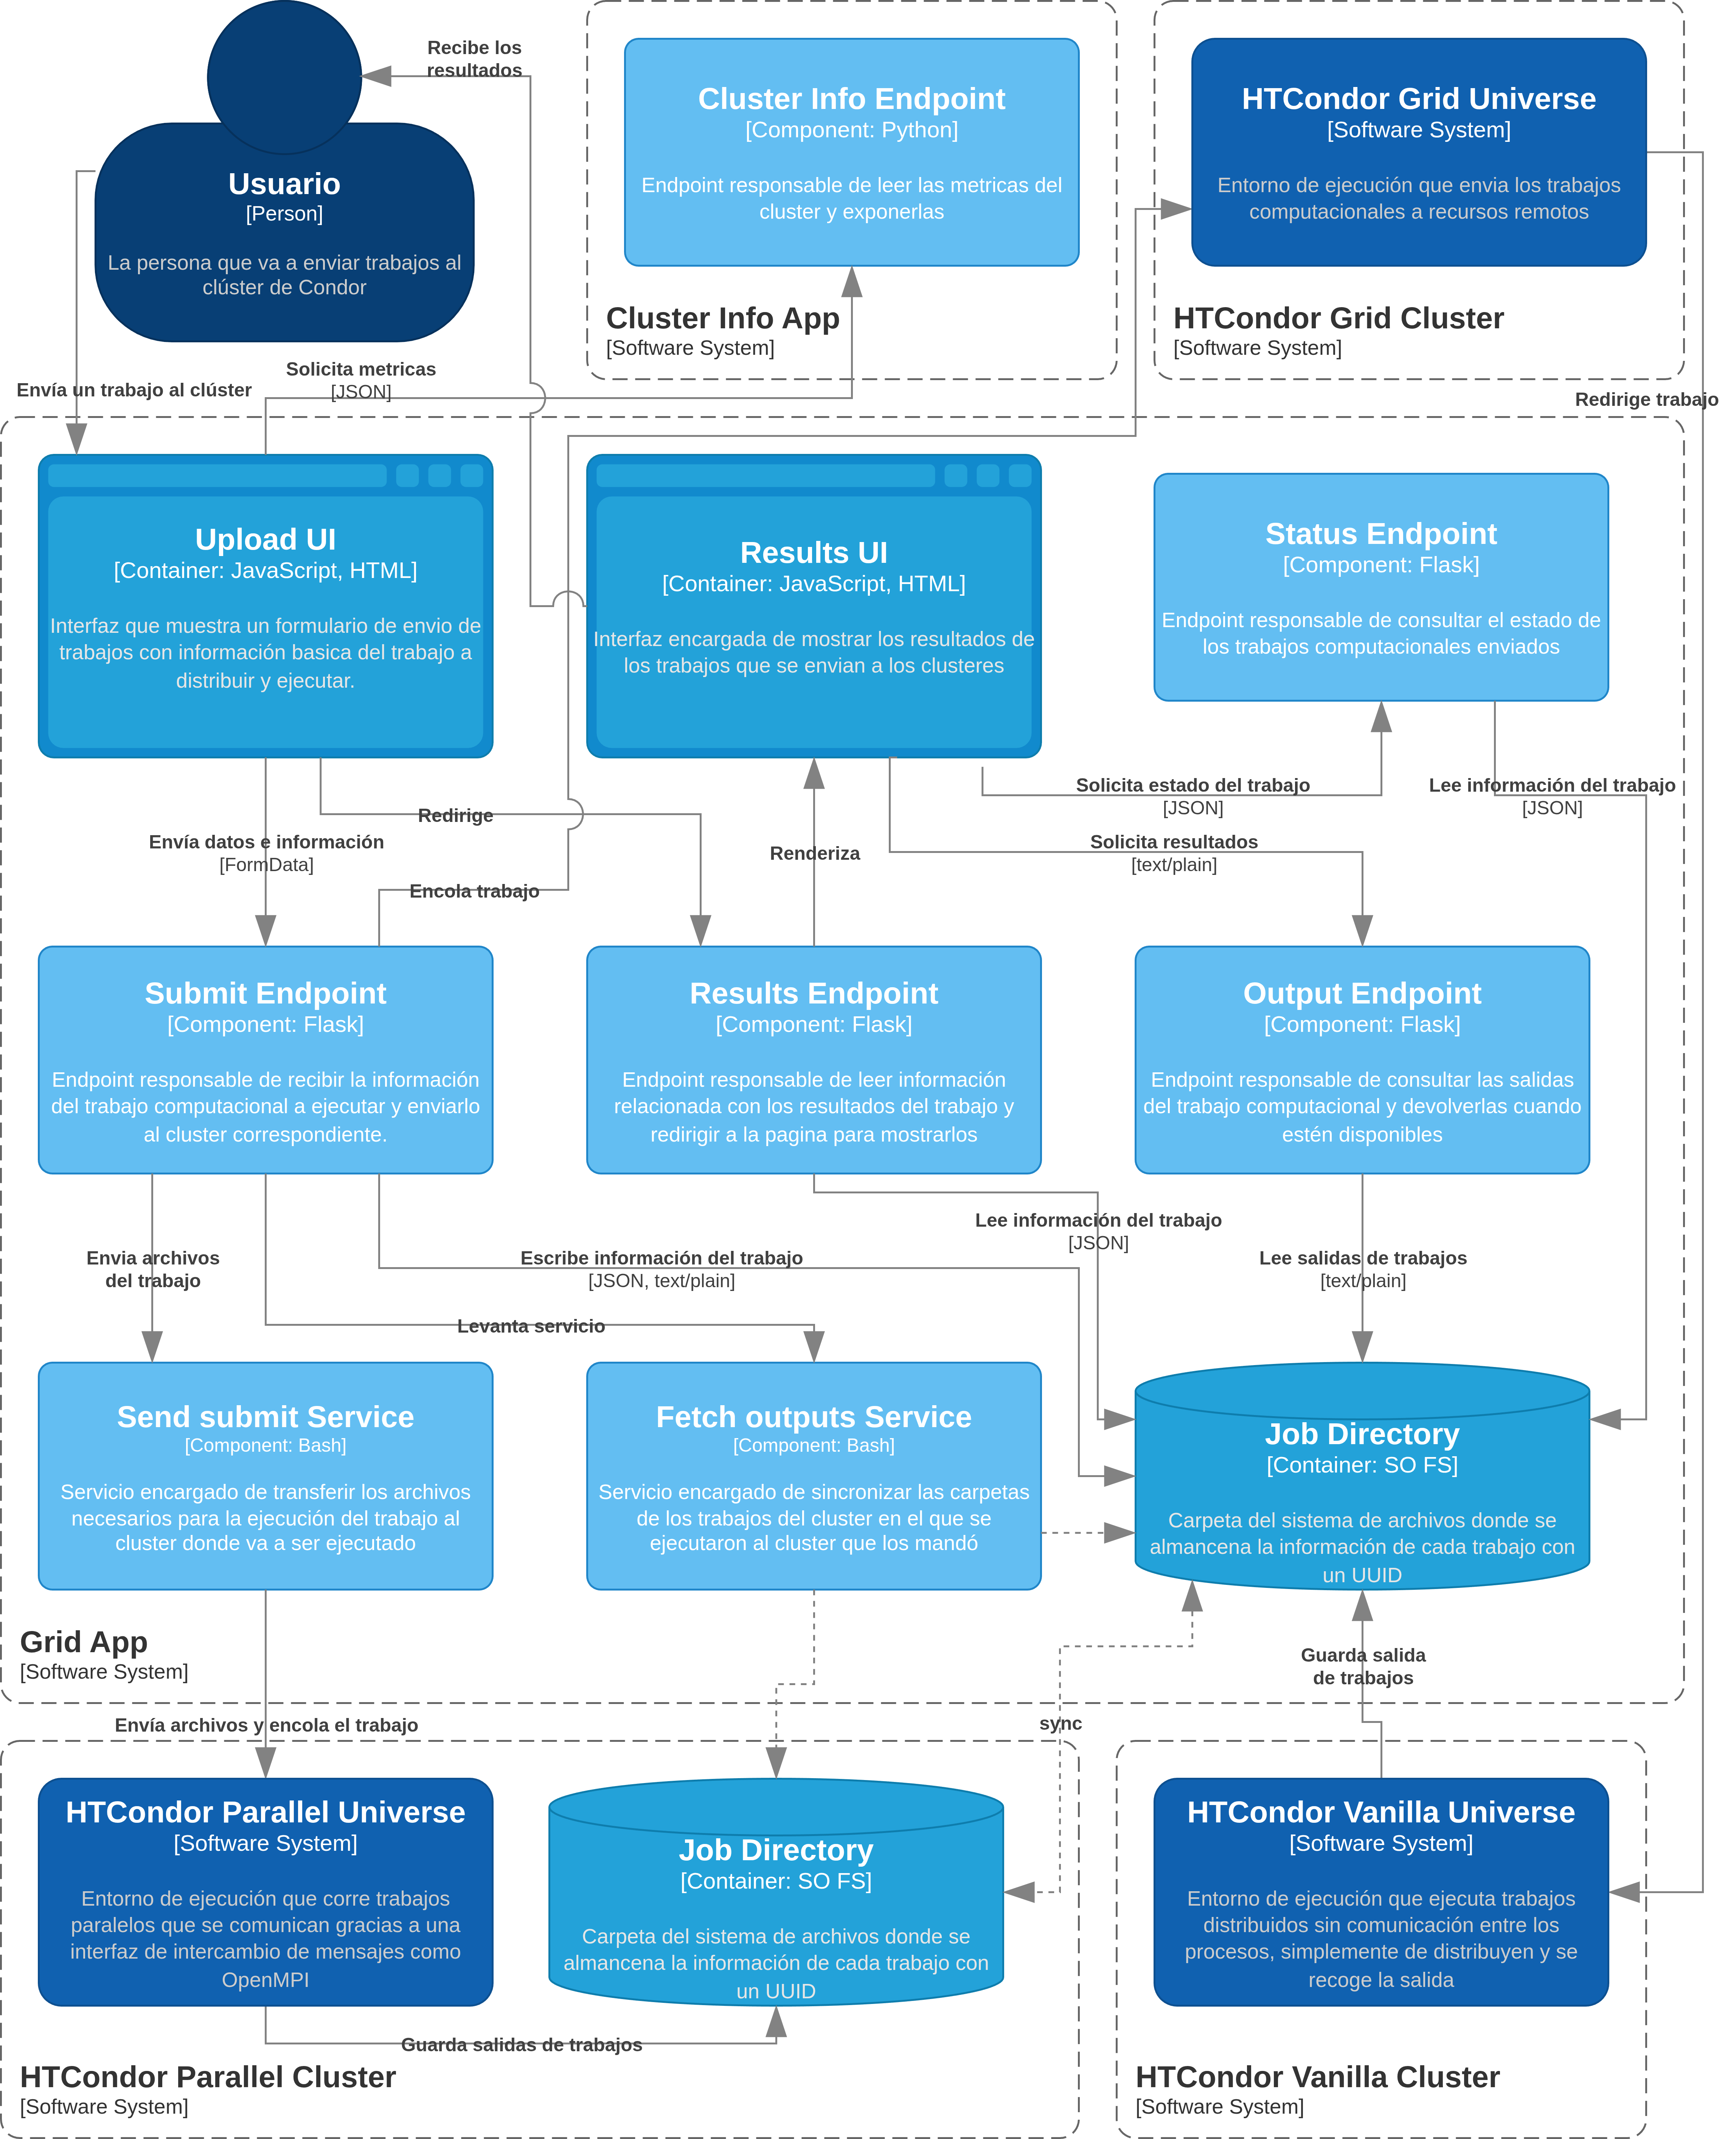
\includegraphics[scale=0.09]{tablas-images/C4/Diagramas HTCondor-Nivel 3 - Apps.drawio.png}
	\caption{Diagrama de componentes para las aplicaciones que componen el sistema}
    \label{fig:C4Nivel3Apps}
\end{figure}

\section{Modelado de secuencia con UML}
\UML es un lenguaje de modelado orientado a múltiples enfoques como la secuencia de eventos y la estructura de las clases \citep{10.1145/1125944.1125949}. Para el caso de este proyecto se usará para describir de forma concreta y estructurada la secuencia que siguen los componentes del Software en cada momento, así como las alternativas que toma el programa con base en la información disponible. De igual forma, se usará este lenguaje para modelar la estructura de las clases que transportan información a través del programa. Cabe aclarar que el sistema no se diseña con una orientación a objetos estricta. Sin embargo su forma principal de intercambio de información es a través de \JSON. Por lo que se hace necesario conocer y describir la forma de los objetos que se intercambian.

\subsection{Diagrama de secuencia}
\noindent
En la Figura \ref{fig:UMLSecuencia} se muestran los procesos y llamados que se ejecutan en cada paso del sistema, desde las rutas que se visitan hasta la información que se transfiere en cada momento. Es importante añadir que la información de transferencia entre cada sistema de software es meramente ilustrativa y para dar mayor profundidad a dicha información, debe complementarse con el diagrama de clases presentado en la sección siguiente y el código de la aplicación presentado en el Apéndice XX.

\begin{figure}[H]
	\centering
	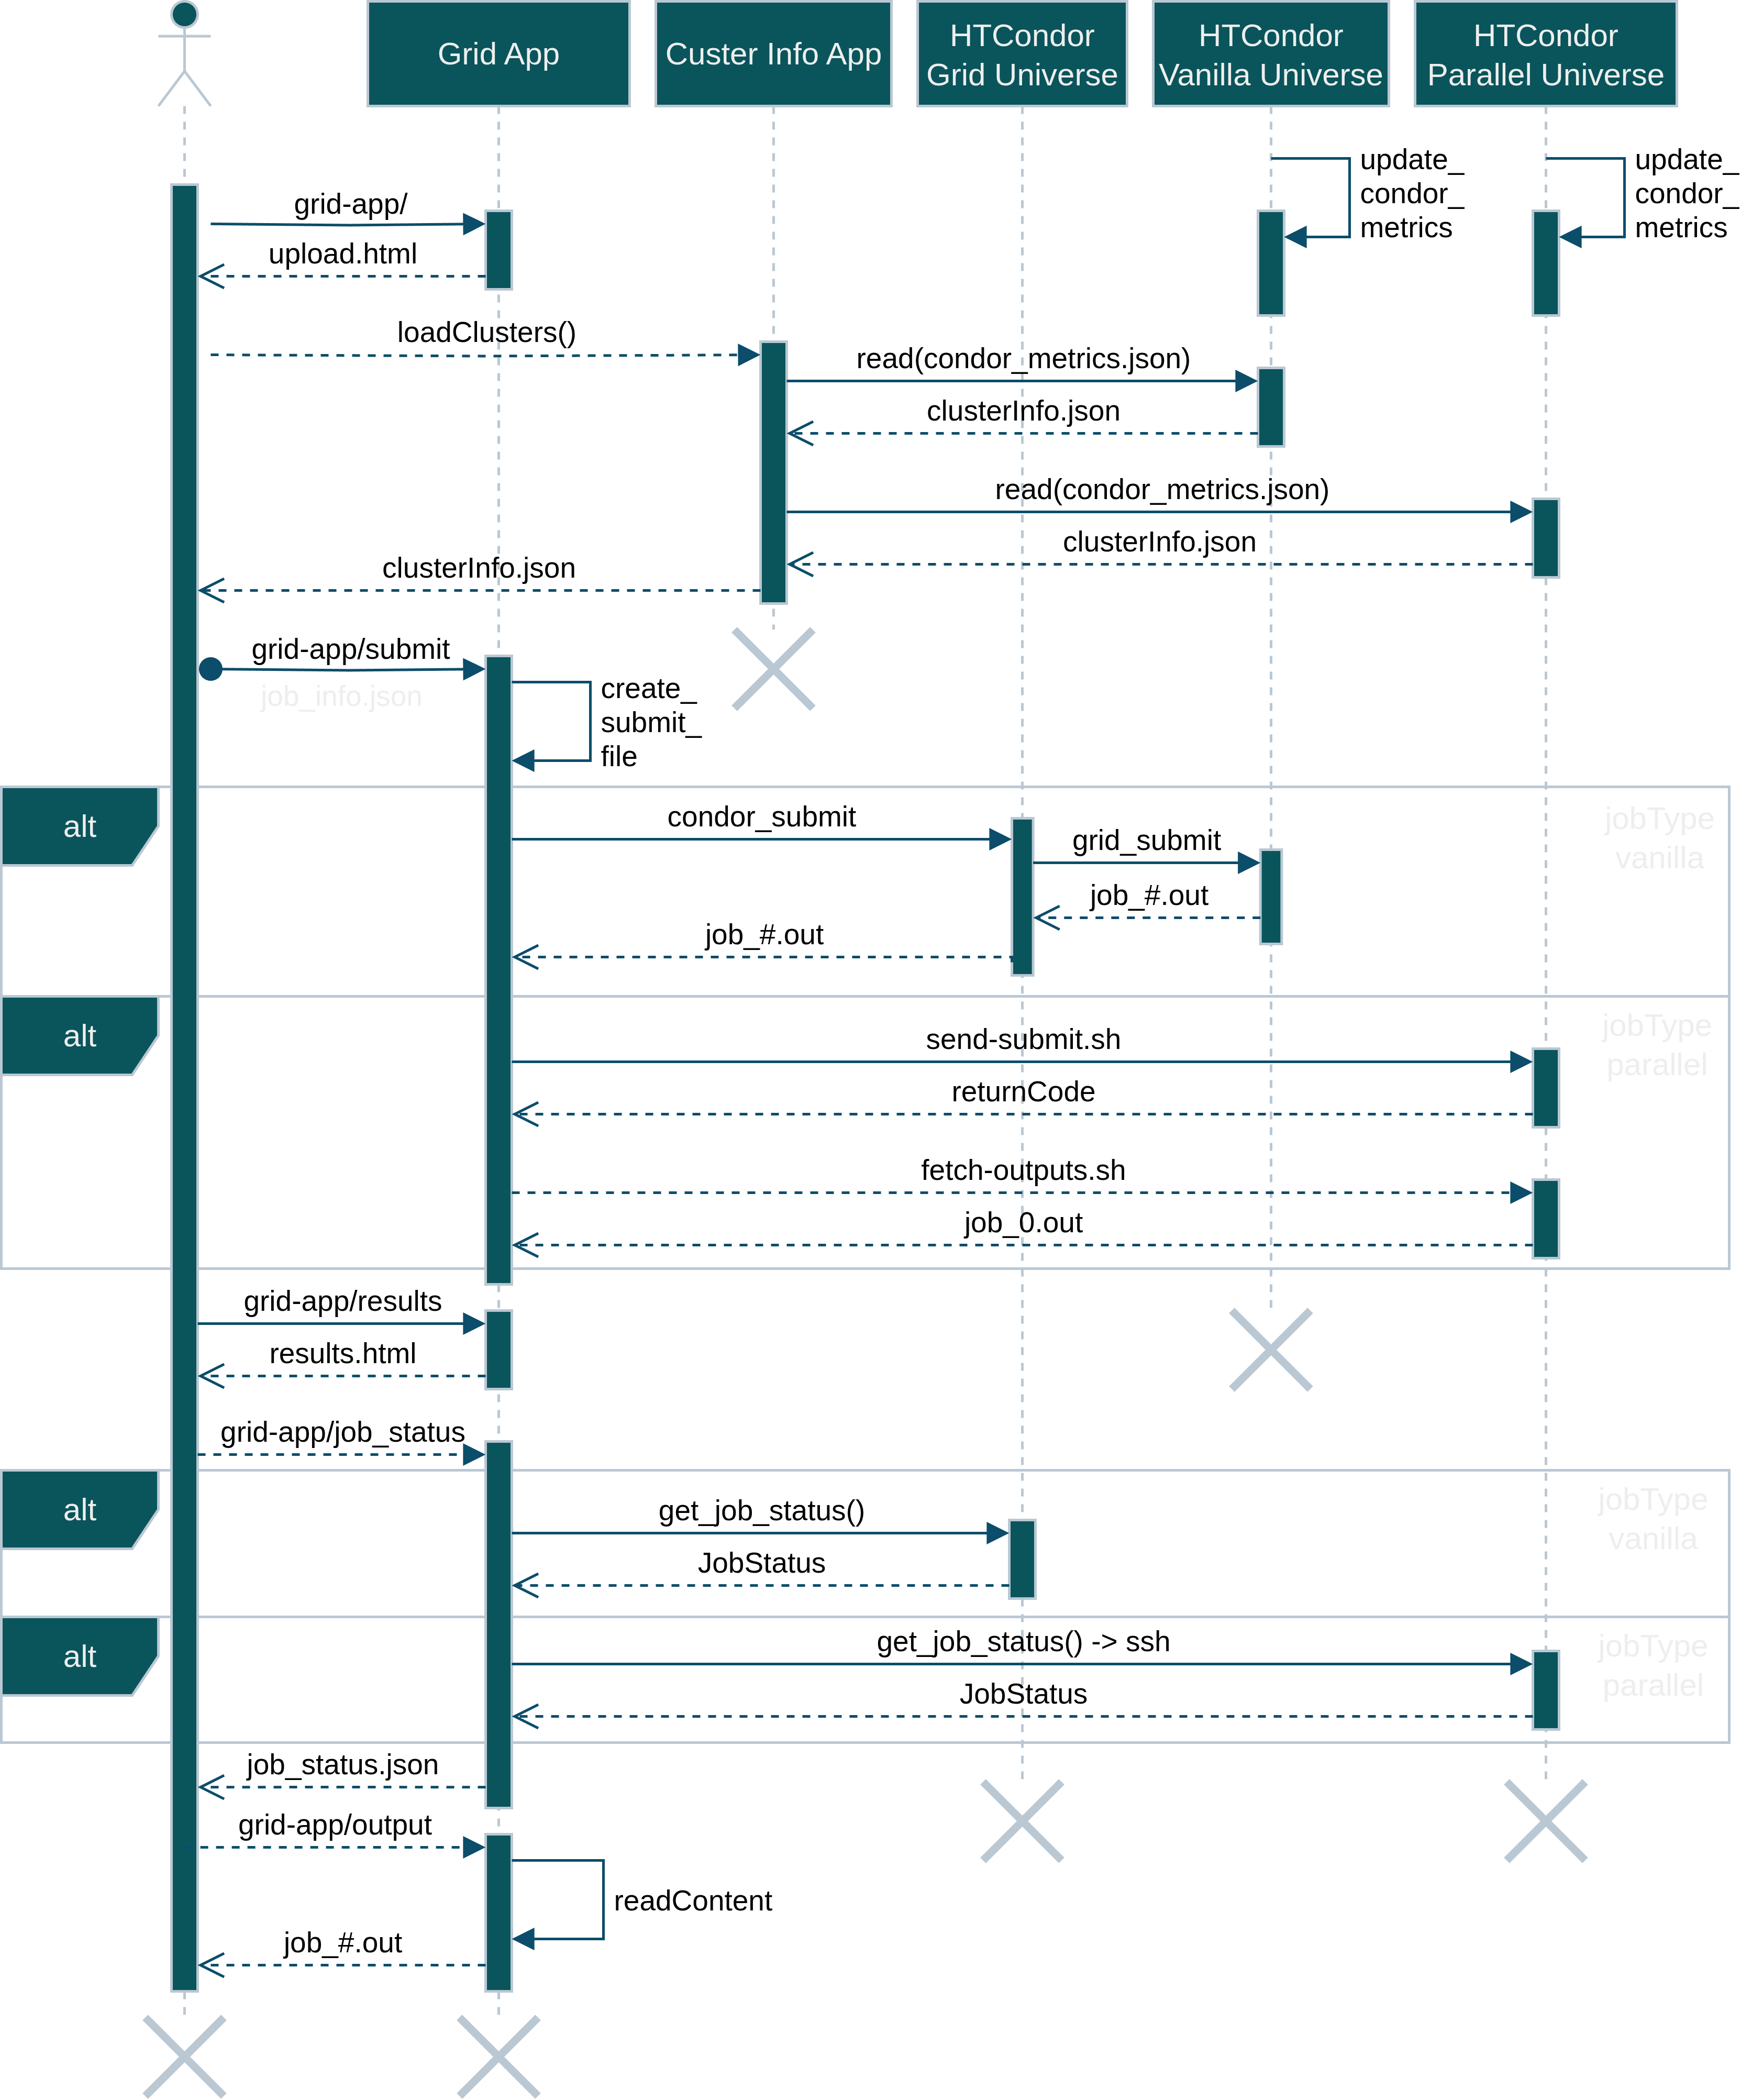
\includegraphics[scale=0.11]{tablas-images/UML/Diagramas HTCondor-Secuencia.drawio.png}
	\caption{Diagrama de secuencia para el sistema}
    \label{fig:UMLSecuencia}
\end{figure}

\subsection{Diagrama de clases}
\noindent
En la Figura \ref{fig:UMLClases} se muestra la composición de las clases en las que se basan los objetos que permiten intercambiar información a través de los sistemas. Debido a que el diseño no fue orientado a objetos, este diagrama solo pretende mostrar los elementos de información que intercambia el sistema y no pretende modelar la arquitectura general de los sistemas de software.

\begin{figure}[H]
	\centering
	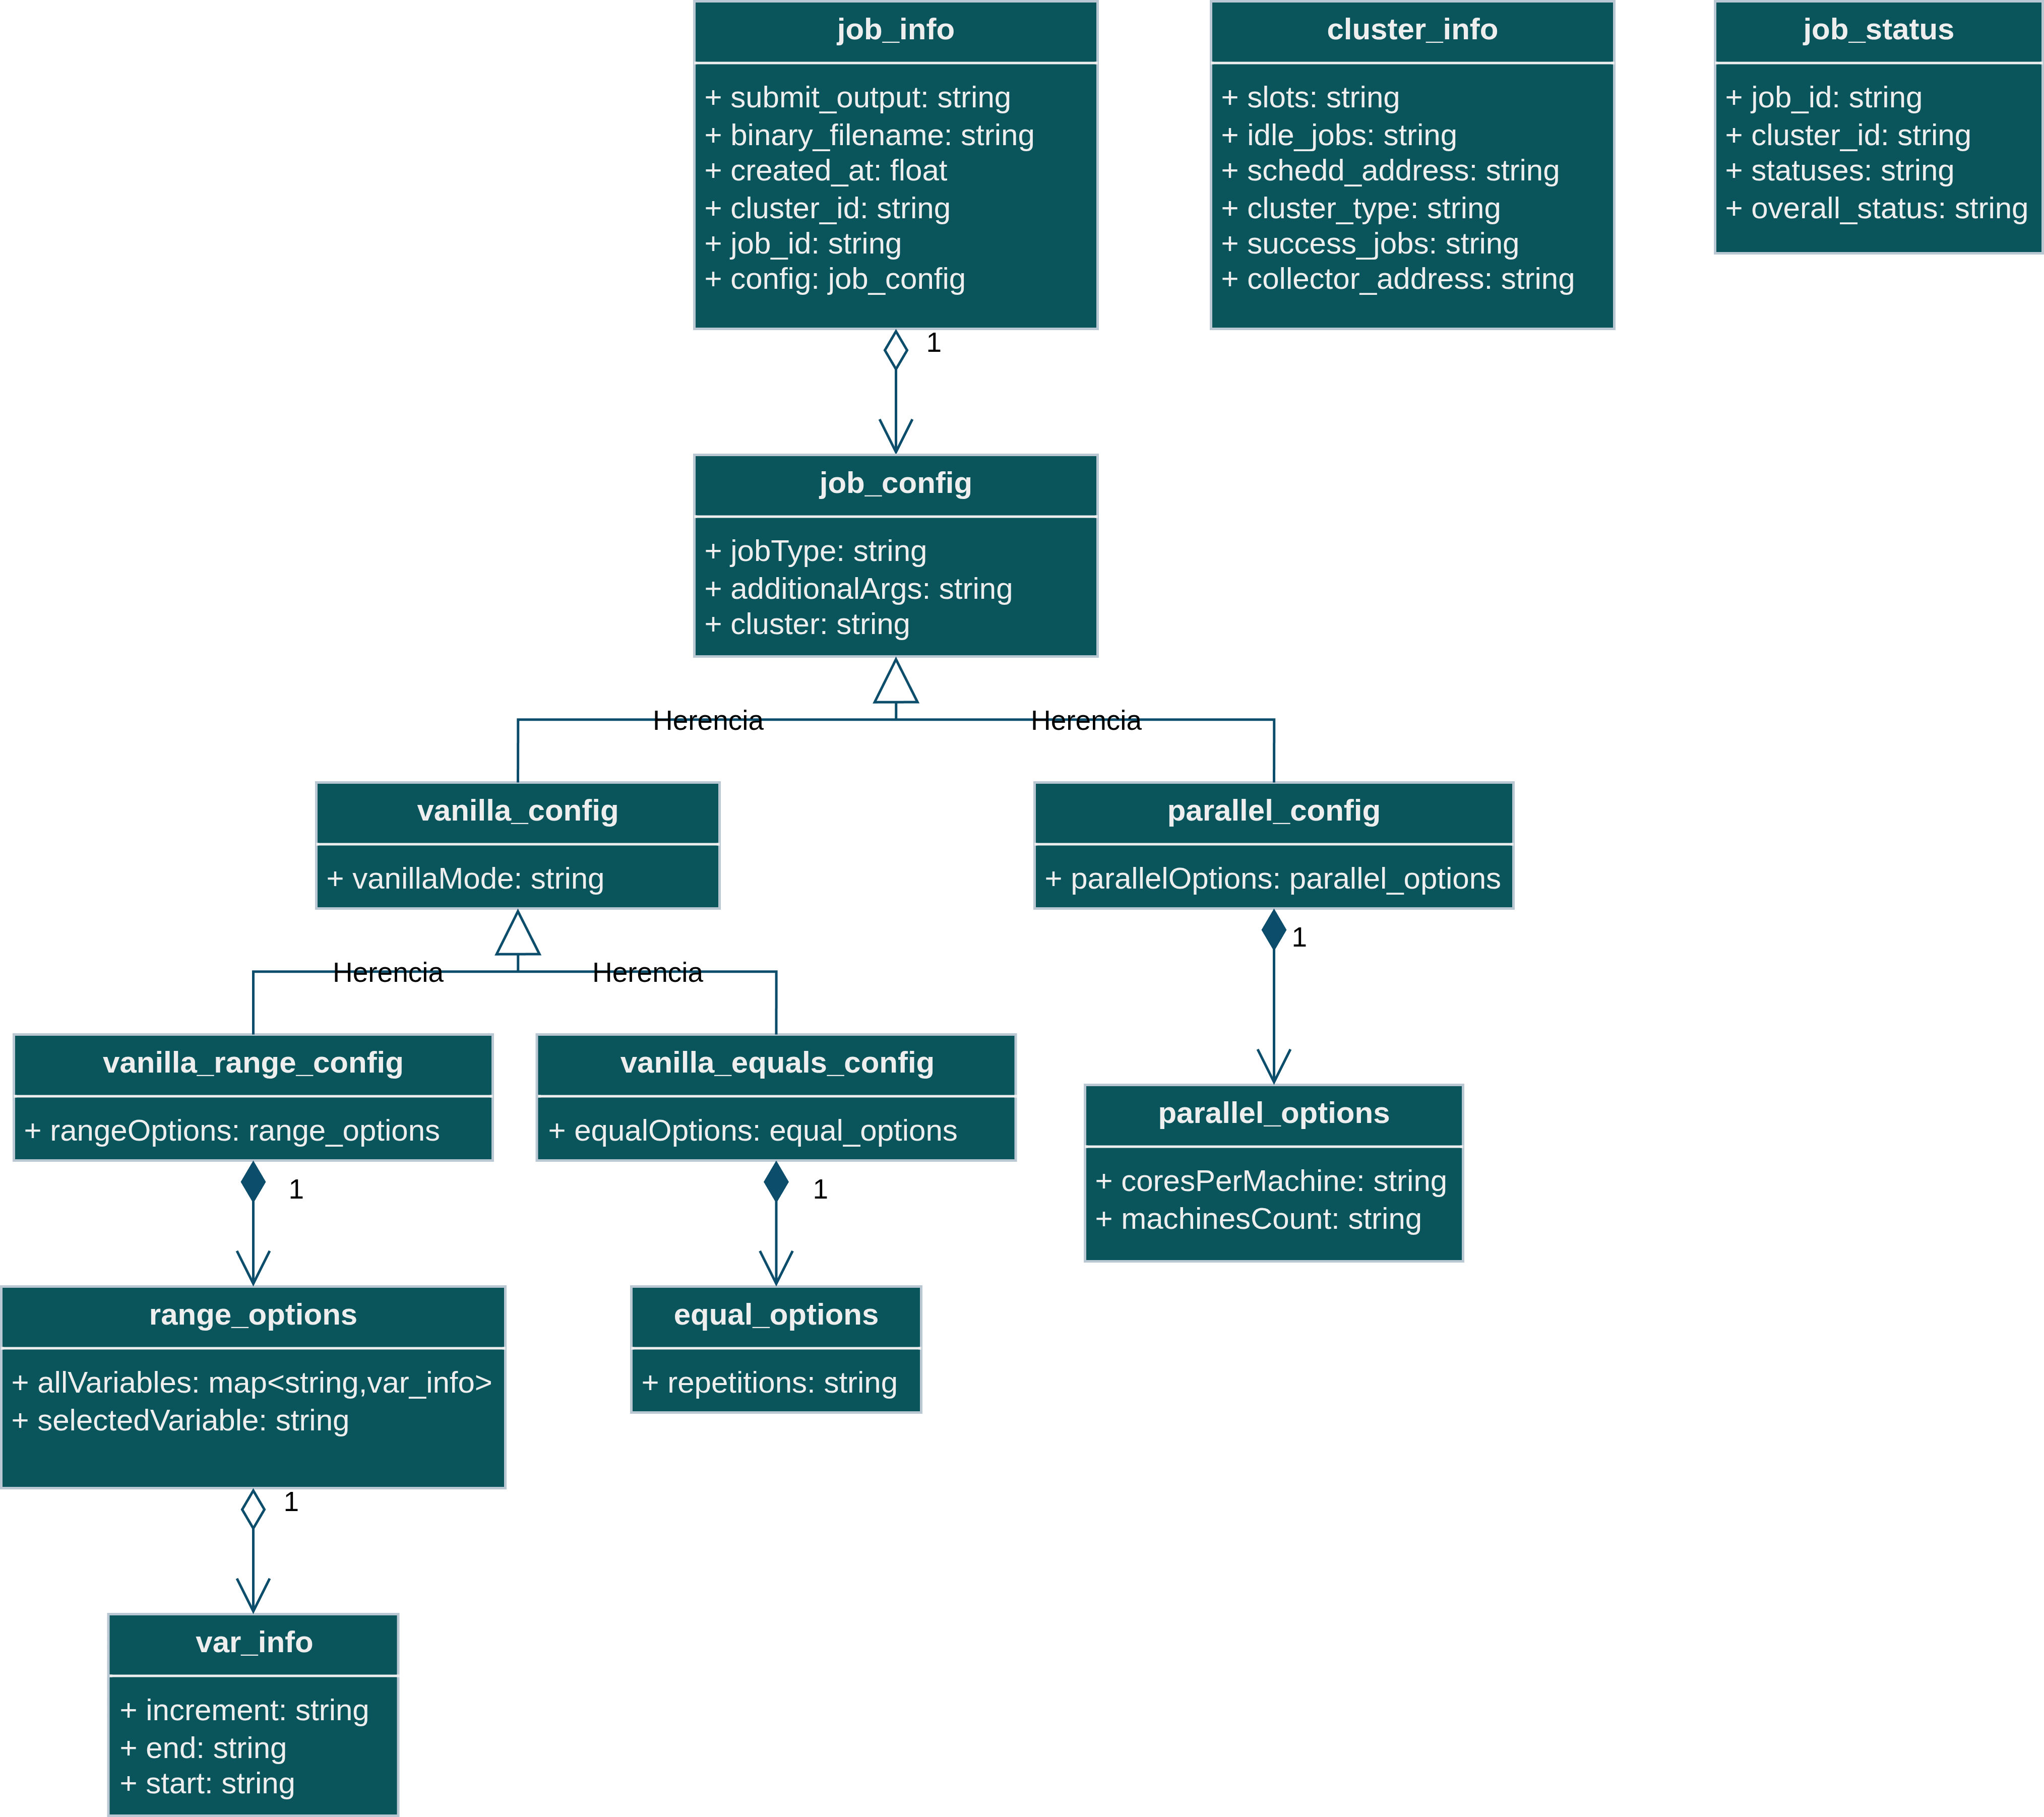
\includegraphics[scale=0.1]{tablas-images/UML/Diagramas HTCondor-Objetos.drawio.png}
	\caption{Diagrama de clases para el sistema}
    \label{fig:UMLClases}
\end{figure}

\section{Modelado de infraestructura con modelos personalizados}
Después de conocer como está compuesto el sistema de forma transversal con ArchiMate y en cuanto a software con C4 y \UML, se hace necesario un modelado más profundo de la infraestructura física y de red que compone la solución. Esto debido a que ArchiMate no da la profundidad necesaria para modelar esta clase de elementos, por lo que se opta por otras opciones con el fin de dar más profundidad al diseño y más claridad al lector sobre los elementos que componen la solución.

A pesar de esto, el equipo del proyecto no halló ningún lenguaje de modelado ni sistema formal que se armonizara con la clase de modelado de infraestructura que se pretende realizar. Por lo que se opta por usar una herramienta de modelado llamada draw.io y figuras genéricas con información complementaria que permiten tener una idea general de la infraestructura que subyace la solución.

\subsection{Modelo de infraestructura física}
\noindent
En la Figura \ref{fig:Fisica} se muestran los componentes de hardware principales que componen la solución. A su vez, se presentan las conexiones eléctricas que tiene cada elemento. Esto con el fin de mostrar la forma en que están conectados a la red eléctrica los componentes, ya que su conexión no es trivial y se hace necesaria documentación especializada que muestre este tipo de elementos.

\begin{figure}[H]
	\centering
	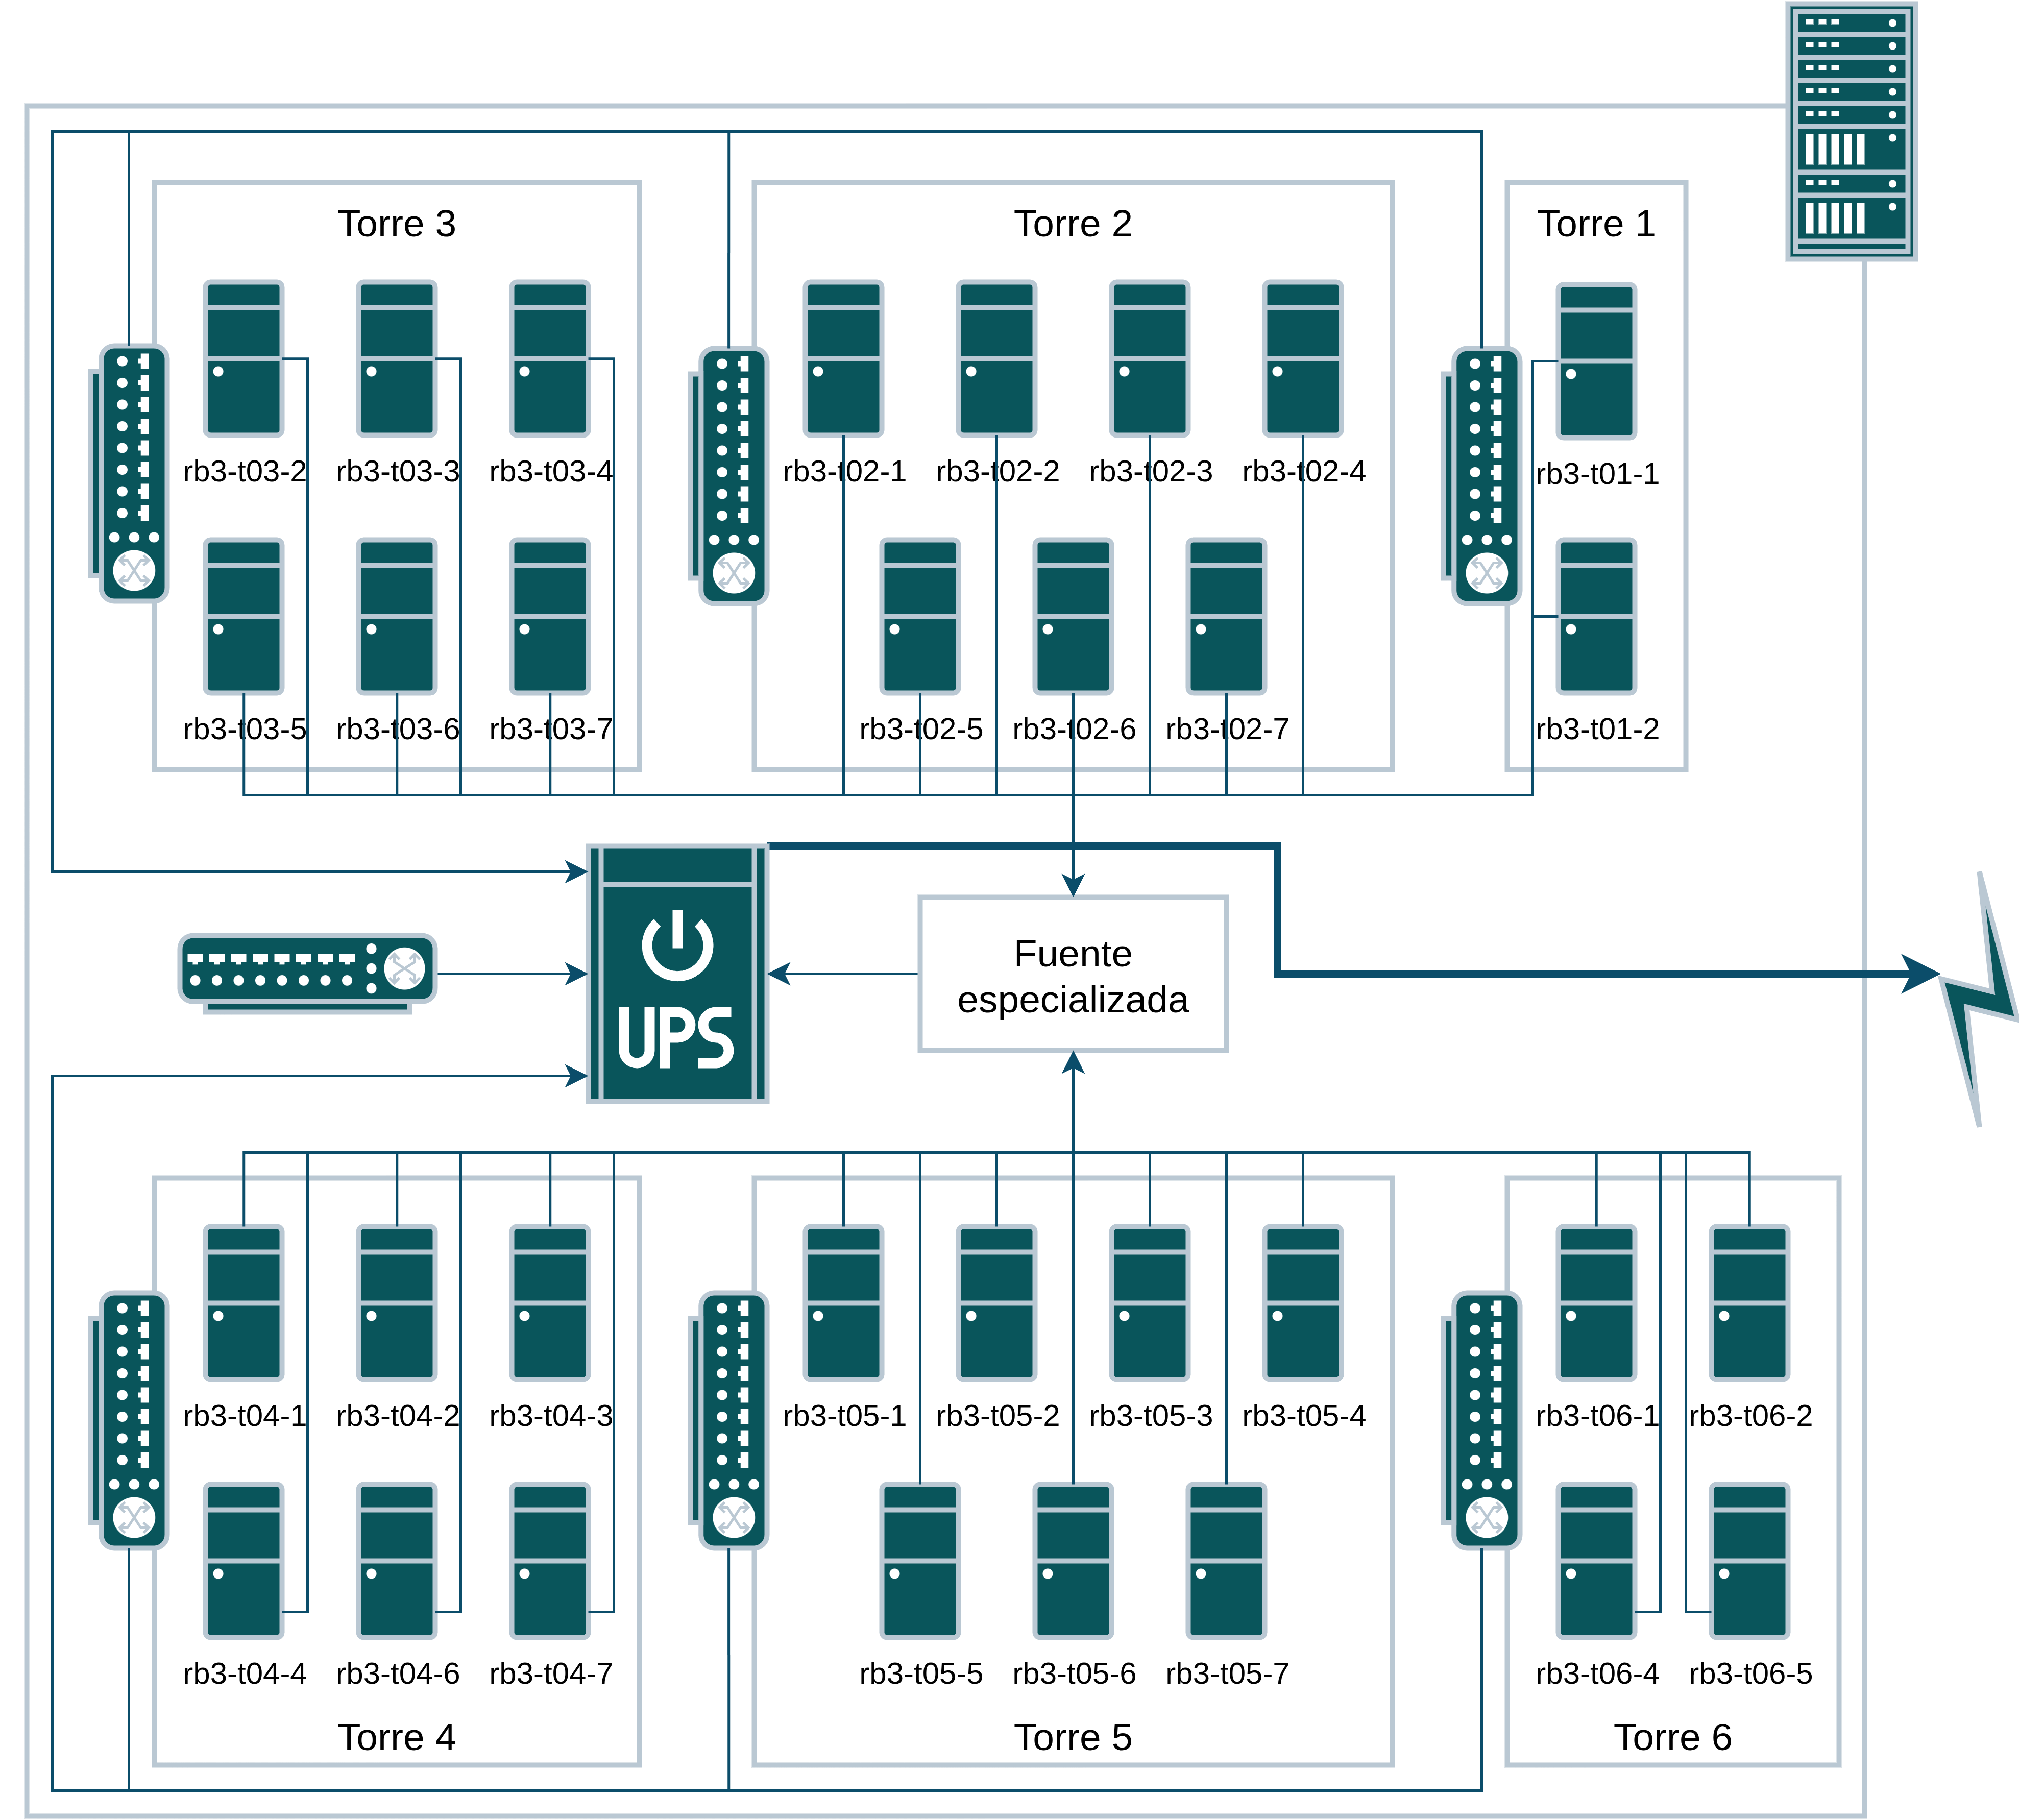
\includegraphics[scale=0.1]{tablas-images/personalizado/Diagramas HTCondor-Fisica.drawio.png}
	\caption{Modelo de infraestructura física}
    \label{fig:Fisica}
\end{figure}

\subsection{Modelo de enlace de datos}
\noindent
En la Figura \ref{fig:Enlace} se muestran las conexiones de red que tiene cada elemento. Esto con el fin de mostrar la forma en que están conectados los componentes a la red y a Internet, ya que su conexión no es trivial y se hace necesaria documentación especializada que muestre estás conexiones.

\begin{figure}[H]
	\centering
	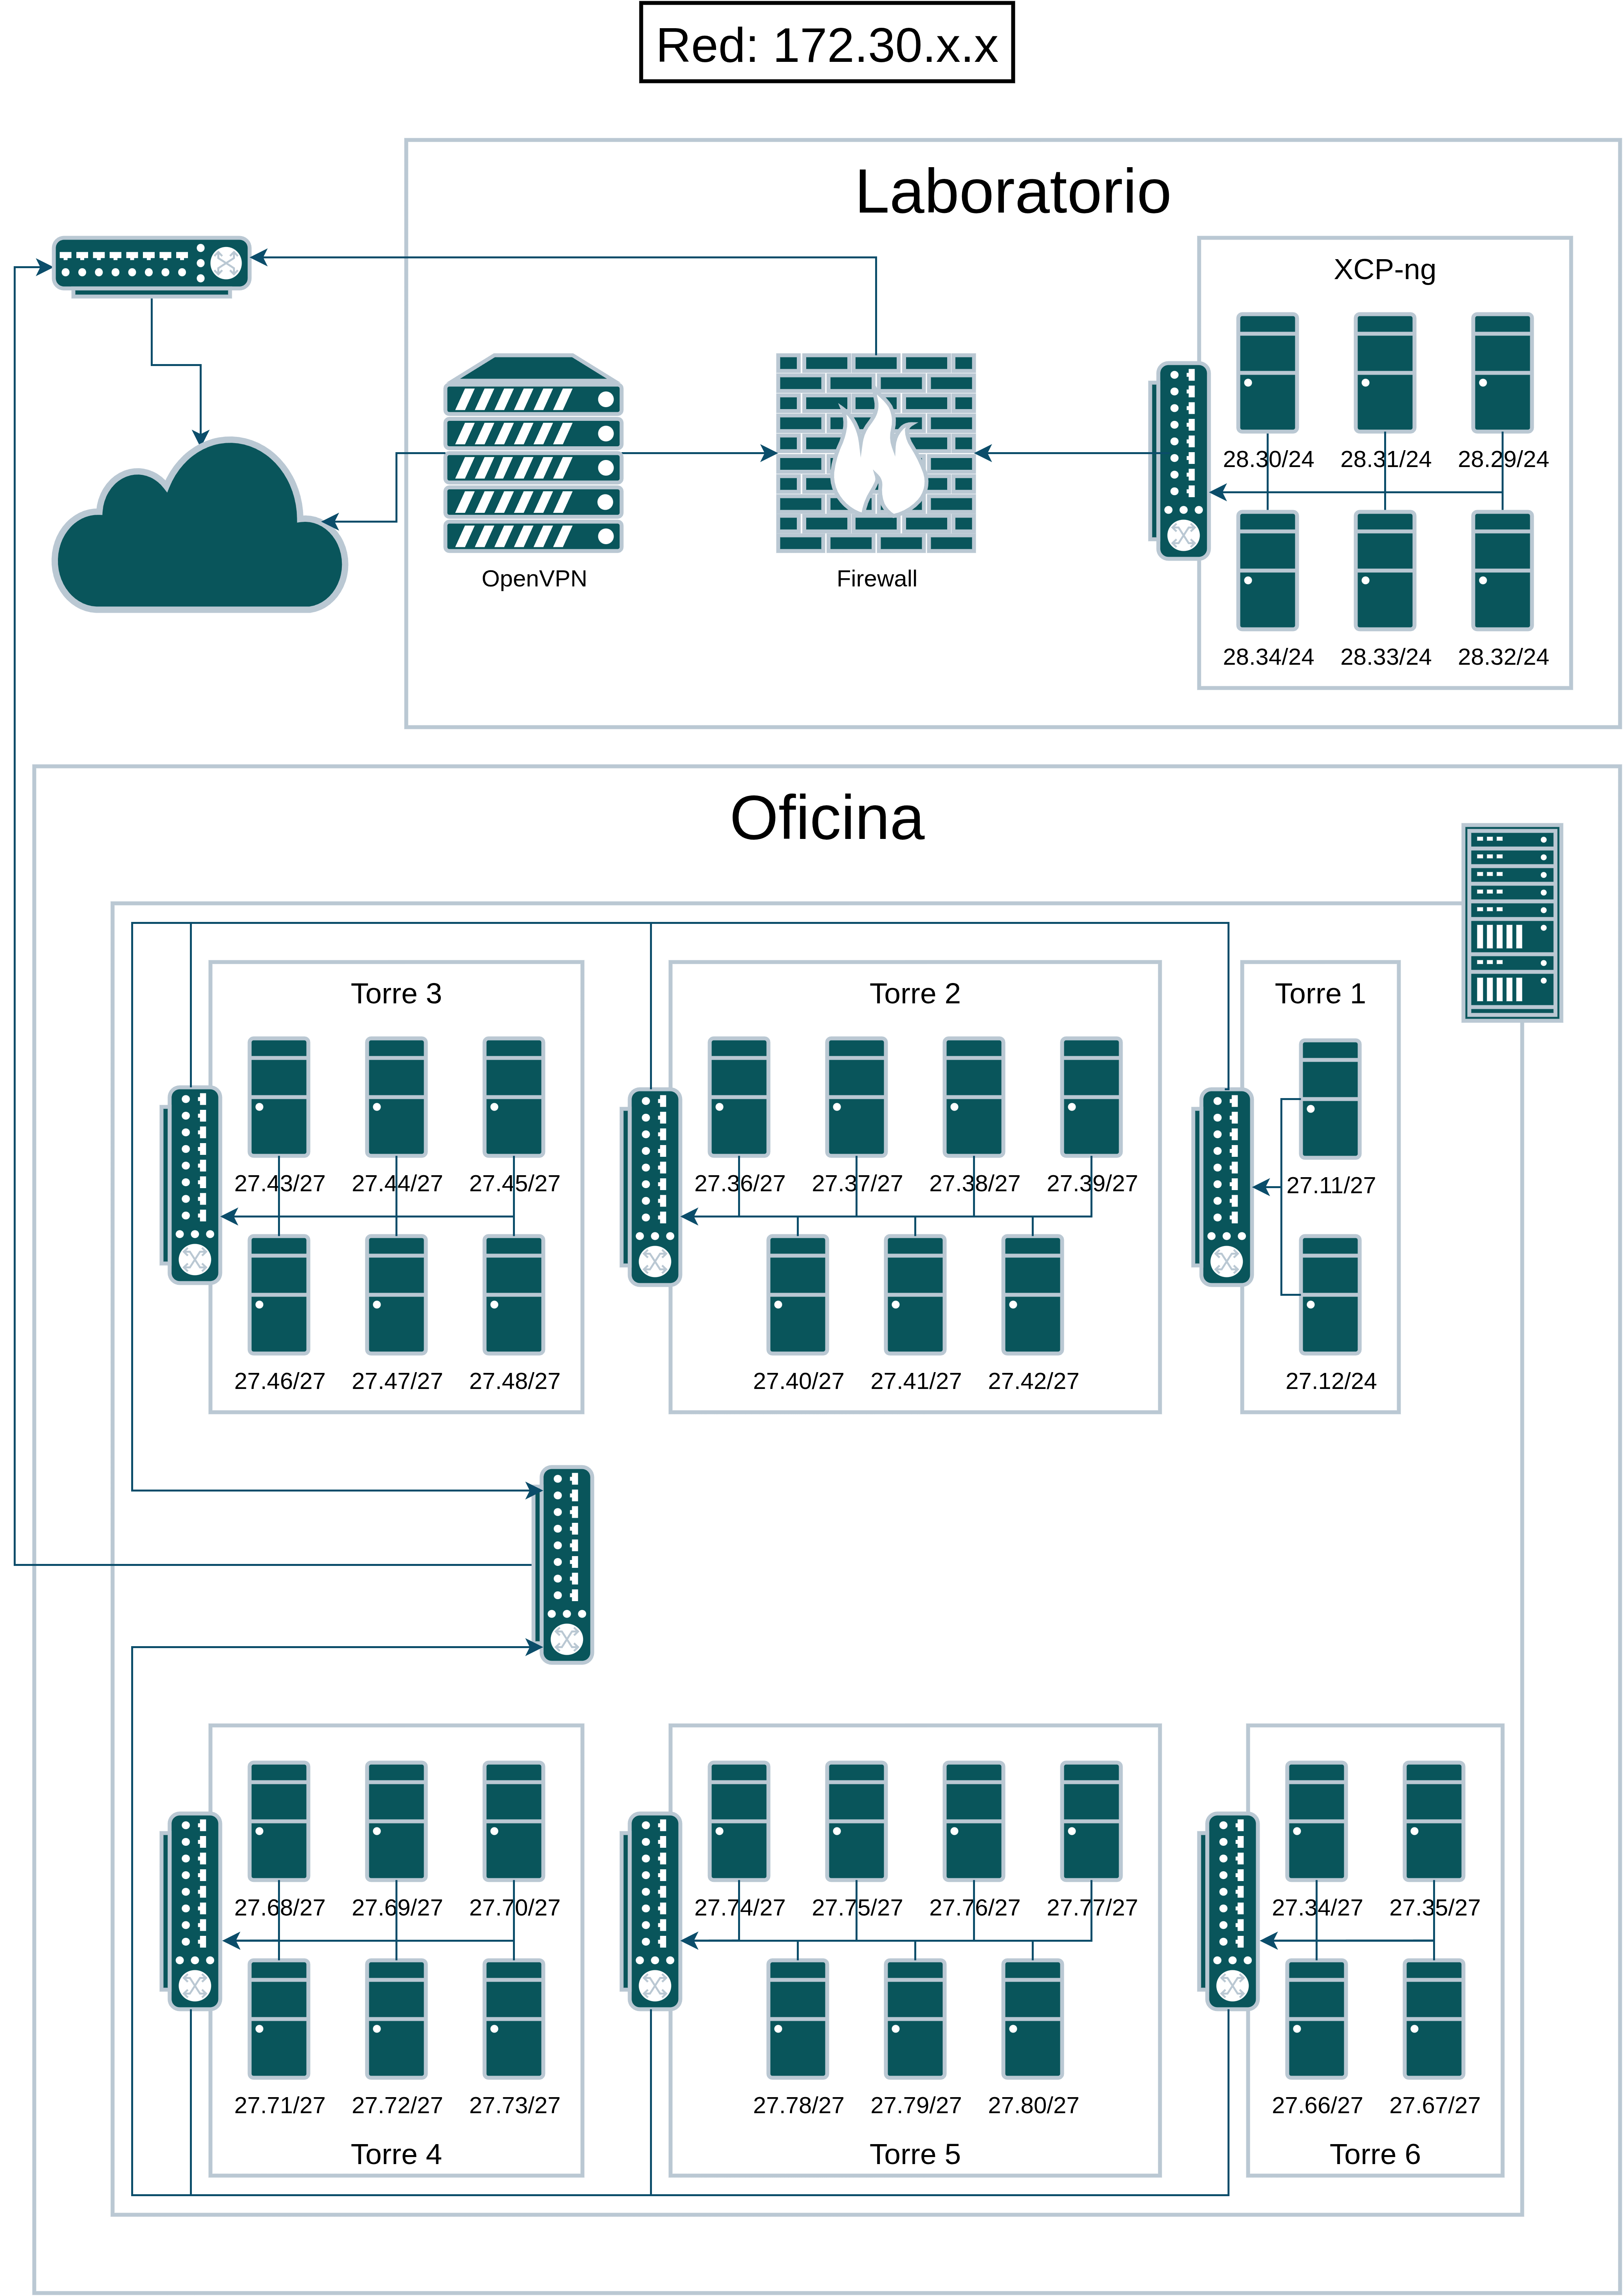
\includegraphics[scale=0.1]{tablas-images/personalizado/Diagramas HTCondor-Enlace.drawio.png}
	\caption{Modelo de enlace de datos}
    \label{fig:Enlace}
\end{figure}

\subsection{Modelo de roles}
\noindent
Después de conocer como están conectados los elementos de infraestructura a nivel eléctrico y de red, se hace necesario plasmar la forma en que están conectados los elementos de forma lógica, que es la forma en que se comunican los elementos en el diseño de la solución. Además, se hace necesario mostrar los roles de \HTCondor que ocupa cada elemento en su clúster. En la Figura \ref{fig:Roles} se plasman estos aspectos.

\begin{figure}[H]
	\centering
	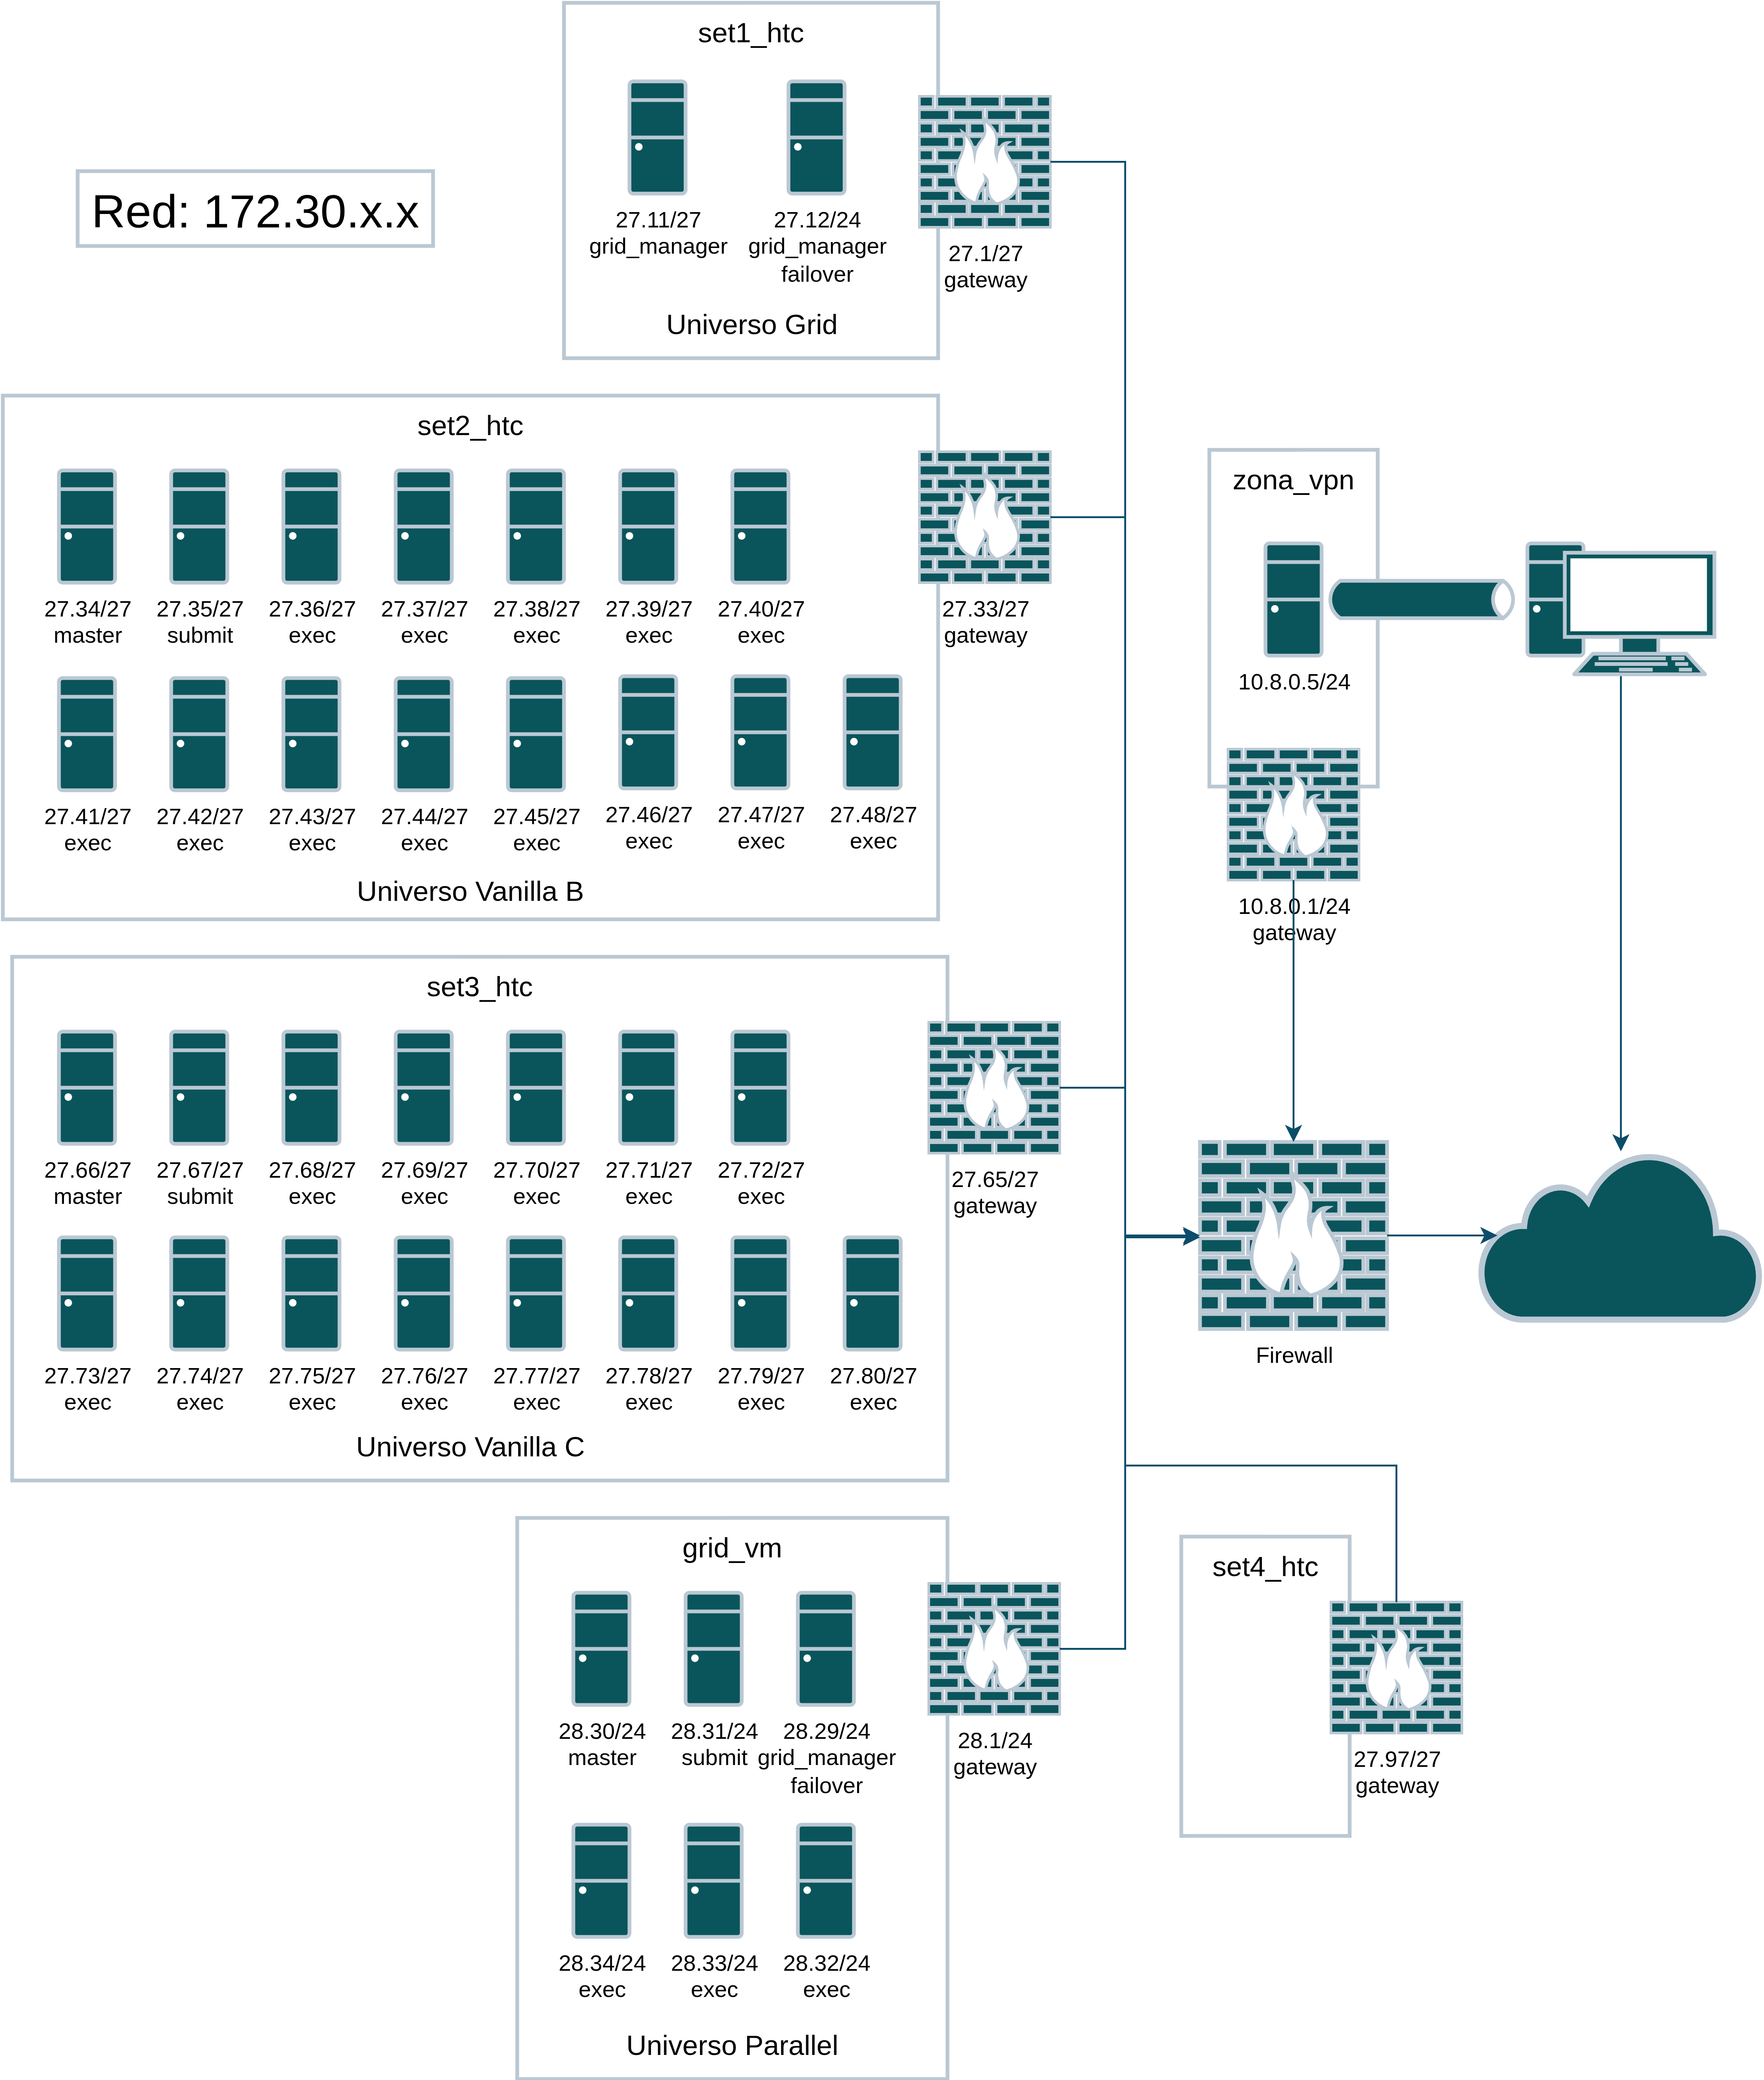
\includegraphics[scale=0.088]{tablas-images/personalizado/Diagramas HTCondor-Roles.drawio.png}
	\caption{Modelo de roles}
    \label{fig:Roles}
\end{figure}
%\ChapterImageStar[cap:pmv]{Producto Mínimo Viable}{./images/fondo.png}\label{cap:pmv}
\mbox{}\\
En este capítulo se implementará el sistema propuesto en la infraestructura HTCondor del Grupo \GRID. Además, se enunciarán las características de cada componente del sistema, su contenido, requisitos y guía de instalación, para hacer un entorno repetible y escalable.

Cabe destacar que para este proyecto se usó Git para el control de versiones, GitHub para gestión de repositorios y se usó un enfoque hacia versionamiento semántico o \textit{SemVer}. Por lo que se mostrarán las aplicaciones y se mencionará la última versión funcional de la aplicación con un \textit{tag}.

\section{\textit{Grid App}}
\noindent
Como se mencionó en el capítulo de diseño de la solución, la aplicación \textit{Grid App} constituye la piedra angular del sistema, funcionando como la interfaz central que permite a los usuarios interactuar con la infraestructura HTCondor distribuida. Esta aplicación web desarrollada en Flask permite cargar trabajos computacionales, configurar parámetros de ejecución específicos para diferentes tipos de universos HTCondor, y visualizar los resultados de manera organizada y accesible.

\subsection{Estructura del proyecto}
\noindent
La aplicación \textit{Grid App} está organizada siguiendo las mejores prácticas de desarrollo web con Flask:

\begin{itemize}
	\item \textbf{app.py}: Archivo principal que contiene la lógica del servidor Flask, incluyendo todos los \textit{endpoints}, manejo de archivos, generación de \textit{submit files} y lógica de interacción con HTCondor.
	
	\item \textbf{templates/}: Directorio que contiene las plantillas \HTML para la interfaz de usuario:
	\begin{itemize}
		\item \texttt{upload.html}: Interfaz principal para la carga y configuración de trabajos.
		\item \texttt{results.html}: Interfaz para visualización de resultados con sistema de pestañas dinámicas.
	\end{itemize}
	
	\item \textbf{static/}: Directorio para archivos estáticos (CSS, JavaScript, imágenes) que proporcionan estilo e interactividad a la aplicación web.
	
	\item \textbf{submits/}: Directorio de trabajo donde se almacenan todos los archivos relacionados con cada trabajo:
	\begin{itemize}
		\item Archivos ejecutables subidos por el usuario.
		\item Archivos de entrada (para trabajos paralelos).
		\item \textit{Submit files} generados automáticamente.
		\item Archivos de salida y \textit{logs} de HTCondor.
		\item Metadatos del trabajo en formato \JSON.
	\end{itemize}
	
	\item \textbf{scripts/}: Directorio que contiene scripts auxiliares de Bash para operaciones específicas:
	\begin{itemize}
		\item \texttt{seno-submit.sh}: Envío de trabajos a clústeres remotos vía SSH.
		\item \texttt{fetch-outputs.sh}: Sincronización de archivos de salida desde clústeres remotos.
	\end{itemize}
\end{itemize}

\begin{figure}[H]
	\centering
	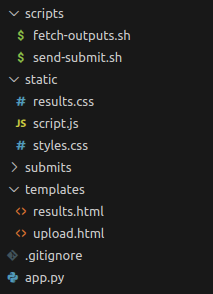
\includegraphics[scale=0.7]{tablas-images/pmv/estructura-proyecto-grid-app.png}
	\caption{Estructura del proyecto \textit{Grid App}}
	\label{fig:estructura-proyecto-grid-app}
\end{figure}

\subsection{Código fuente}
\noindent

% TODO: Actualizar información del repositorio, rama y versión
El código fuente de la aplicación \textit{Grid App} está disponible en el repositorio correspondiente y su implementación se presenta en los apéndices de este documento. La aplicación está desarrollada completamente en Python utilizando el \textit{framework} Flask para el \textit{backend} y HTML/CSS/JavaScript para la interfaz de usuario.

\subsection{Características técnicas y configuración}
\noindent

\subsubsection{Configuración de la aplicación}
\noindent

La aplicación \textit{Grid App} utiliza las siguientes configuraciones globales definidas en \texttt{app.py}:

\begin{itemize}
	\item \textbf{DEFAULT\_PROJECT\_FOLDER}: Directorio base de la aplicación, configurable entre desarrollo y producción.
	\item \textbf{SUBMIT\_FOLDER}: Directorio para almacenamiento de trabajos (\texttt{/submits/}).
	\item \textbf{SCRIPTS\_FOLDER}: Directorio de scripts auxiliares (\texttt{/scripts/}).
	\item \textbf{JOB\_STATUS}: Diccionario global para traducción de códigos de estado HTCondor.
\end{itemize}

\subsubsection{Manejo de archivos y permisos}
\noindent

El sistema implementa un manejo robusto de archivos:

\begin{itemize}
	\item \textbf{Permisos ejecutables}: Los archivos binarios reciben permisos \texttt{0o755} automáticamente.
	\item \textbf{Codificación de archivos}: Lectura de salidas con \texttt{encoding='utf-8', errors='ignore'}.
	\item \textbf{Gestión de directorios}: Creación automática con \texttt{os.makedirs(job\_dir, exist\_ok=True)}.
\end{itemize}

\subsubsection{Concurrencia y \textit{multithreading}}
\noindent

Para trabajos paralelos, la aplicación utiliza \textit{threading} para operaciones no bloqueantes:

\begin{verbatim}
def traer_salidas():
    subprocess.run(['./fetch-outputs.sh', job_dir, submit_ip, job_id], ...)

thread = threading.Thread(target=traer_salidas)
thread.start()
\end{verbatim}

\subsection{Componentes de la interfaz web}
\noindent

\subsubsection{\textit{Upload Interface}}
\noindent
Interfaz principal implementada en \texttt{upload.html}, servida por el \textit{endpoint} raíz. Proporciona un formulario \textit{multipart} para carga de archivos y configuración de parámetros de ejecución específicos por tipo de universo HTCondor.

\begin{figure}[H]
	\centering
	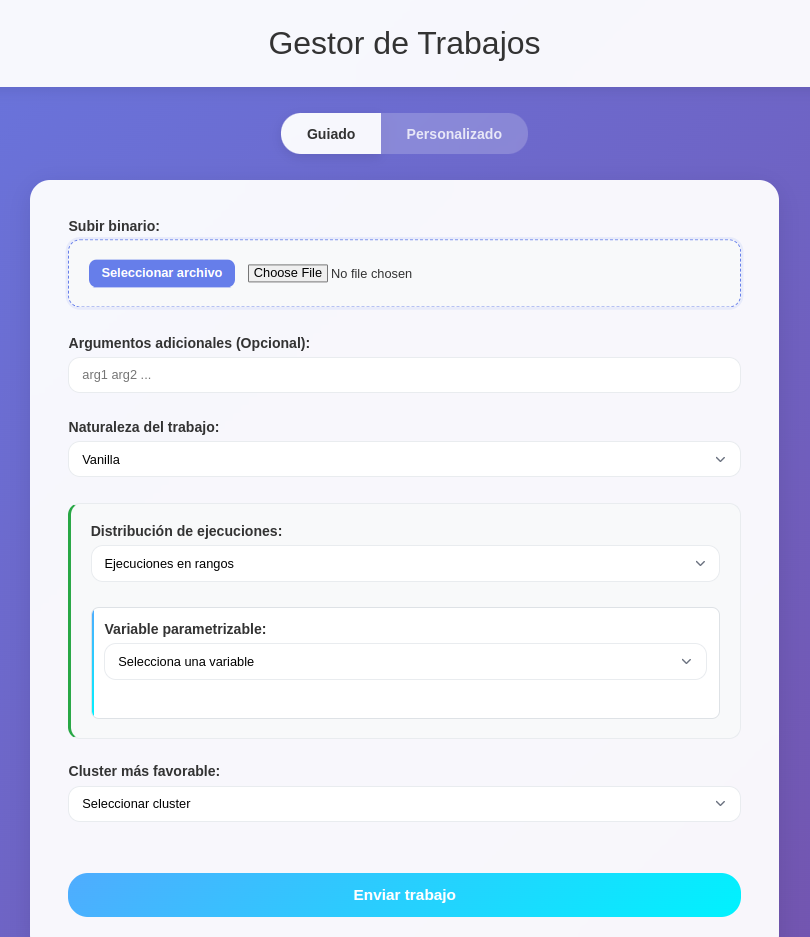
\includegraphics[scale=0.5]{tablas-images/pmv/upload-ui-screenshot.png}
	\caption{Interfaz de carga de trabajos}
	\label{fig:uiCargasTrabajos}
\end{figure}

\subsubsection{\textit{Results Interface}}
\noindent
Interfaz dinámica implementada en \texttt{results.html} que utiliza JavaScript para carga asíncrona de archivos de salida mediante peticiones AJAX al \textit{endpoint} \texttt{/output/<job\_id>/<filename>}. Presenta información completa del trabajo y sistema de pestañas para navegación entre múltiples archivos de salida.

\begin{figure}[H]
	\centering
	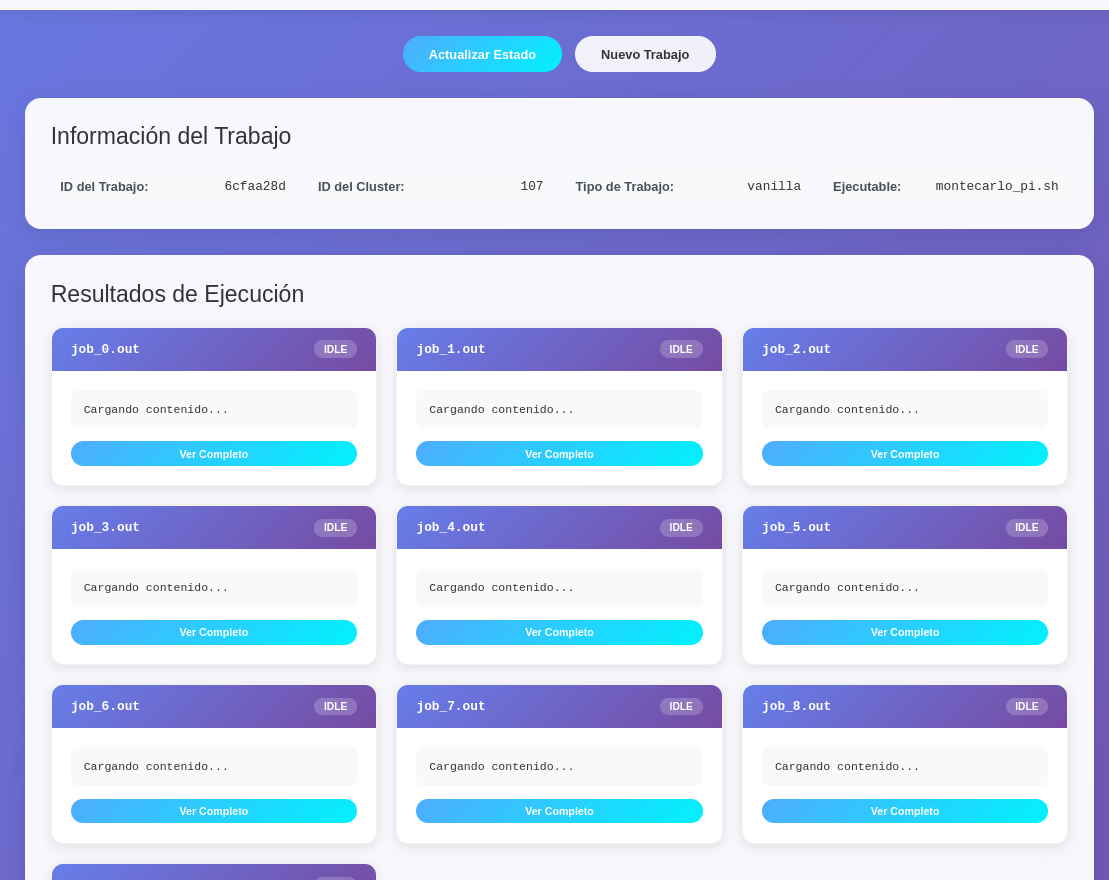
\includegraphics[scale=0.35]{tablas-images/pmv/results-ui-screenshot.png}
	\caption{Interfaz de resultados de trabajos}
	\label{fig:uiResultadosTrabajos}
\end{figure}

\subsection{Componentes \textit{backend} (\textit{endpoints})}
\noindent

La aplicación \textit{Grid App} está implementada como una aplicación Flask que expone múltiples \textit{endpoints} para gestionar el ciclo de vida completo de los trabajos computacionales en HTCondor. El servidor Flask se ejecuta por defecto en el puerto \texttt{5000} y está configurado para aceptar conexiones desde cualquier interfaz de red (\texttt{host='0.0.0.0'}). Los \textit{endpoints} principales del sistema se describen a continuación.

\subsubsection{Root Endpoint (/)}
\noindent

El \textit{Root Endpoint} sirve la página principal de la aplicación. Este \textit{endpoint} está expuesto en la ruta raíz (\texttt{/}) y acepta peticiones de tipo GET.

\textbf{Funcionamiento:}

Renderiza la plantilla HTML \texttt{upload.html} que contiene la interfaz principal para la carga y configuración de trabajos computacionales.

\subsubsection{Submit Endpoint (/submit)}
\noindent

El \textit{Submit Endpoint} es el componente más complejo del sistema, responsable de procesar la información del trabajo computacional y coordinarlo con los diferentes tipos de universos HTCondor. Este \textit{endpoint} está expuesto en la ruta \texttt{/submit} y acepta peticiones de tipo \texttt{POST}.

\textbf{Funcionamiento:}

\begin{enumerate}
	\item \textbf{Generación del identificador único}: Genera un UUID de 8 caracteres utilizando \texttt{str(uuid.uuid4())[:8]} para identificar únicamente cada trabajo.

	\item \textbf{Procesamiento de archivos}: Recibe y procesa hasta tres archivos opcionales del formulario multipart:
	      \begin{itemize}
		      \item \texttt{binary-file}: Ejecutable principal del trabajo.
		      \item \texttt{input-file}: Archivo de entrada (requerido para trabajos parallel).
		      \item \texttt{submit-file}: Submit file personalizado de HTCondor.
	      \end{itemize}

	\item \textbf{Configuración del trabajo}: Parsea la configuración JSON que incluye:
	      \begin{itemize}
		      \item \texttt{jobType}: Especifica el universo (\texttt{'vanilla'} o \texttt{'parallel'}).
		      \item \texttt{cluster}: Dirección del clúster de destino.
		      \item \texttt{additionalArgs}: Argumentos para el ejecutable.
		      \item \texttt{vanillaMode}: Modo de distribución para trabajos vanilla ('range' o 'equal').
		      \item \texttt{rangeOptions}: Configuración de variables y rangos.
		      \item \texttt{parallelOptions}: Configuración de máquinas y núcleos.
	      \end{itemize}

	\item \textbf{Generación automática de submit files}: La función \texttt{create\_submit\_file()} genera diferentes tipos de submit files:

	      \textbf{Para universo Grid (Vanilla):}
	      \begin{itemize}
		      \item Configura \texttt{universe = grid} y \texttt{grid\_resource = condor}.
		      \item Establece requisitos de arquitectura: \texttt{requirements = (Arch == ``armv7l'')}.
		      \item Maneja distribución de trabajos:
		            \begin{itemize}
			            \item \textit{Modo range}: Genera trabajos explícitos con variables iterativas.
			            \item \textit{Modo equal}: Crea trabajos idénticos con \texttt{queue N}.
		            \end{itemize}
	      \end{itemize}

	      \textbf{Para universo Parallel:}
	      \begin{itemize}
		      \item Configura \texttt{universe = parallel}.
		      \item Utiliza \texttt{executable = /usr/share/doc/condor/examples/openmpiscript}.
		      \item Establece \texttt{machine\_count} y \texttt{request\_cpus}.
		      \item Configura variables de entorno OpenMPI.
		      \item Establece política de apagado: \texttt{+ParallelShutdownPolicy = ``WAIT\_FOR\_NODE0''}.
	      \end{itemize}

	\item \textbf{Ejecución de trabajos}:

	      \textbf{Trabajos Vanilla:} Ejecuta \texttt{condor\_submit} directamente en el directorio local del trabajo.

	      \textbf{Trabajos Parallel:} 
	      \begin{itemize}
		      \item Ejecuta el script \texttt{send-submit.sh} para transferir archivos al clúster remoto.
		      \item Inicia un hilo separado con \texttt{threading.Thread} que ejecuta \texttt{fetch-outputs.sh}.
	      \end{itemize}

	\item \textbf{Extracción del cluster ID}: Utiliza la expresión regular \texttt{r``(\\textbackslash{}d+)\\textbackslash{}s+job\\textbackslash{}(s\\textbackslash{})\\textbackslash{}s+submitted to cluster\\textbackslash{}s+(\\textbackslash{}d+)''} para extraer el ID del clúster de la salida de \texttt{condor\_submit}.

	\item \textbf{Persistencia de metadatos}: Guarda \texttt{job\_info.json} con información completa del trabajo, incluyendo configuración, timestamps y salida de HTCondor.
\end{enumerate}

\textbf{Respuesta:}

Retorna un JSON con la estructura:

\begin{verbatim}
{
  "success": true,
  "job_id": "a1b2c3d4", 
  "cluster_id": "123",
  "message": "Trabajo enviado exitosamente"
}
\end{verbatim}

\subsubsection{Job Status Endpoint (/job\_status/<job\_id>)}
\noindent

Este endpoint consulta el estado actual de un trabajo en los sistemas HTCondor correspondientes, manejando tanto trabajos locales (vanilla) como remotos (parallel).

\textbf{Funcionamiento:}

\begin{enumerate}
	\item \textbf{Validación}: Verifica la existencia de \texttt{job\_info.json} y extrae el \texttt{cluster\_id}.

	\item \textbf{Consulta de estado}: Ejecuta comandos específicos según el tipo de trabajo:

	      \textbf{Trabajos Vanilla:}
	      \begin{verbatim}
condor_q {cluster_id} -long | grep -E '^JobStatus'
	      \end{verbatim}

	      \textbf{Trabajos Parallel:}
	      \begin{verbatim}
ssh -i ~/.ssh/parallel alma@{submit_ip} 
  "condor_q {cluster_id} -long | grep -E '^JobStatus'"
	      \end{verbatim}

	\item \textbf{Consulta en historial}: Si no se encuentra en \texttt{condor\_q}, consulta \texttt{condor\_history} con \texttt{-limit 1}.

	\item \textbf{Procesamiento de estados}: Utiliza el diccionario global \texttt{JOB\_STATUS} para traducir códigos numéricos:

	      \begin{table}[H]
		      \centering
		      \begin{tabular}{|c|l|}
			      \hline
			      \textbf{Código} & \textbf{Estado}        \\
			      \hline
			      1               & Idle                   \\
			      2               & Running                \\
			      3               & Removed                \\
			      4               & Completed              \\
			      5               & Held                   \\
			      \hline
		      \end{tabular}
		      \caption{Códigos de estado de HTCondor}
		      \label{tab:job-status-codes}
	      \end{table}

	\item \textbf{Determinación del estado general}:
	      \begin{itemize}
		      \item \texttt{all(s == ``Completed'' for s in statuses)}: Estado ``Completed''.
		      \item \texttt{``Running'' in statuses}: Estado ``Running''.
		      \item \texttt{len(set(statuses)) > 1}: Estado ``Mixed''.
		      \item Caso contrario: Primer estado de la lista.
	      \end{itemize}
\end{enumerate}

\textbf{Respuesta:}

\begin{verbatim}
{
  "job_id": "a1b2c3d4",
  "cluster_id": "123", 
  "statuses": ["Running", "Completed"],
  "overall_status": "Running"
}
\end{verbatim}

\subsubsection{Results Endpoint (/results/<job\_id>)}
\noindent

Este endpoint renderiza la página de visualización de resultados con un sistema dinámico de pestañas para múltiples archivos de salida.

\textbf{Funcionamiento:}

\begin{enumerate}
	\item \textbf{Validación}: Verifica la existencia del directorio del trabajo.

	\item \textbf{Carga de metadatos}: Lee \texttt{job\_info.json} para obtener la configuración del trabajo.

	\item \textbf{Identificación de archivos de salida}:

	      \textbf{Trabajos Vanilla:}
	      \begin{verbatim}
for filename in os.listdir(job_dir):
    if filename.startswith('job_') and filename.endswith('.out'):
        output_files.append(filename)
output_files.sort()
	      \end{verbatim}

	      \textbf{Trabajos Parallel:}
	      \begin{verbatim}
output_files = ['job_0.out']
	      \end{verbatim}

	\item \textbf{Renderizado}: Utiliza \texttt{render\_template('results.html')} con contexto que incluye \texttt{job\_info}, \texttt{output\_files} y \texttt{job\_id}.
\end{enumerate}

\subsubsection{Output Endpoint (/output/<job\_id>/<filename>)}
\noindent

Endpoint auxiliar que sirve el contenido específico de archivos de salida individuales para carga dinámica mediante AJAX.

\textbf{Funcionamiento:}

\begin{enumerate}
	\item \textbf{Construcción de ruta}: \texttt{os.path.join(job\_dir, filename)}

	\item \textbf{Validación}: \texttt{os.path.exists(output\_path)}

	\item \textbf{Lectura robusta}: 
	      \begin{verbatim}
with open(output_path, 'r') as file:
    content = file.read()
	      \end{verbatim}

	\item \textbf{Respuesta}: \texttt{Response(content, mimetype='text/plain')}
\end{enumerate}

\subsubsection{State Endpoint (/state/<id>)}
\noindent

Endpoint simplificado para consulta rápida de estado por clúster ID (funcionalidad adicional).

\textbf{Funcionamiento:}

Ejecuta \texttt{condor\_q \{id\} -long | grep -E '\^{}JobStatus'} y retorna directamente el estado traducido usando el diccionario \texttt{JOB\_STATUS}.

\subsection{Proceso de instalación}
\noindent

\subsubsection{Descripción general del entorno}
\noindent
Requisitos del sistema para el despliegue de \textit{Grid App}:

\begin{itemize}
	\item Sistema operativo: Raspbian GNU/Linux 9 (stretch) o superior.
	\item Python: Versión 3.6 o superior con pip.
	\item Dependencias Python: Flask y módulos estándar (uuid, threading, subprocess).
	\item HTCondor: Instalación completa con universo Grid configurado.
	\item SSH: Configuración de claves para acceso a clústeres remotos (parallel jobs).
	\item Usuario: Permisos para ejecutar comandos HTCondor y escritura en directorios de trabajo.
\end{itemize}

\subsubsection{Pasos de instalación}
\noindent

% TODO: Actualizar URL del repositorio, rama y comandos de instalación específicos
Instalación de la aplicación:

\begin{enumerate}
	\item Clonar el repositorio:
	      \begin{verbatim}
			git clone [URL_REPOSITORIO] /opt/grid-app
		\end{verbatim}
	
	\item Instalar dependencias Python:
	      \begin{verbatim}
			cd /opt/grid-app
			pip3 install flask
		\end{verbatim}
	
	\item Configurar directorios de trabajo:
	      \begin{verbatim}
			mkdir -p /opt/grid-app/submits
			mkdir -p /opt/grid-app/scripts
			chmod 755 /opt/grid-app/scripts/*.sh
		\end{verbatim}
	
	\item Configurar acceso SSH para trabajos parallel:
	      \begin{verbatim}
			ssh-keygen -t rsa -f ~/.ssh/parallel
			# Copiar clave pública a clústeres remotos
		\end{verbatim}
\end{enumerate}

\subsubsection{Configuración del servicio}
\noindent

Para ejecutar la aplicación como servicio del sistema:

% TODO: Crear script de instalación automatizado similar al de Cluster Info App
\begin{enumerate}
	\item Crear archivo de unidad systemd en \texttt{/etc/systemd/system/grid-app.service}.
	\item Configurar el servicio para ejecutarse en el puerto 5000.
	\item Habilitar y iniciar el servicio con systemctl.
\end{enumerate}

\subsubsection{Mantenimiento automático}
\noindent

Configuración de limpieza periódica del directorio de trabajos:

\begin{enumerate}
	\item Agregar al crontab:
	      \begin{verbatim}
			crontab -e
		\end{verbatim}
	
	\item Agregar tarea de limpieza diaria:
	      \begin{verbatim}
			0 2 * * * find /opt/grid-app/submits \
				-type d -mtime +7 -exec rm -rf {} +
		\end{verbatim}
\end{enumerate}

La configuración presentada representa el entorno específico utilizado durante el desarrollo y puede requerir adaptaciones según las características particulares del sistema de destino y los requisitos de la infraestructura HTCondor existente.

\section{\textit{Cluster Info App}}
\noindent

Como se mencionó en el capítulo de diseño de la solución, la aplicación \textit{Cluster Info App} es la encargada de recopilar métricas del clúster y exponerlas a través de una \API. Es importante añadir que esta aplicación debe correr en la máquina \textit{submit} de cada clúster al que se quieran enviar trabajos, pues es a través de esta que el \textit{grid manager} y la aplicación \textit{Grid App} obtienen la información para redirigir los trabajos y ejecutarlos en los recursos remotos.

\subsection{Estructura del proyecto}
\noindent
La aplicación \textit{Cluster Info App} está compuesta por tres archivos principales que trabajan en conjunto para proporcionar métricas del clúster HTCondor:

\begin{itemize}
	\item \textbf{update\_condor\_metrics.sh}: \textit{Script} de \textit{Bash} que recopila métricas del clúster HTCondor ejecutando comandos específicos de HTCondor y generando un archivo JSON con la información.
	\item \textbf{cluster-info.py}: Servidor HTTP ligero implementado en Python que lee las métricas del archivo JSON y las expone a través de una API REST.
	\item \textbf{install.sh}: \textit{Script} de instalación que configura el servicio como un daemon del sistema usando systemd.
\end{itemize}

\begin{figure}[H]
	\centering
	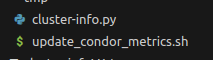
\includegraphics[scale=0.7]{tablas-images/pmv/estructura-proyecto-cluster-info-app.png}
	\caption{Estructura del proyecto \textit{Cluster Info App}}
	\label{fig:estructura-proyecto-cluster-info-app}
\end{figure}

\subsection{Componentes de la aplicación}
\noindent

\subsubsection{Script de recopilación de métricas (update\_condor\_metrics.sh)}
\noindent

Este componente es responsable de ejecutar comandos específicos de HTCondor para recopilar información del estado del clúster y generar un archivo JSON con las métricas. El \textit{script} recopila las siguientes métricas:

\begin{itemize}
	\item \textbf{Slots disponibles}: Utiliza el comando \texttt{condor\_status -avail -total} para obtener el número total de \textit{slots} de CPU disponibles en el clúster.
	
	\item \textbf{Porcentaje de trabajos exitosos}: Calcula el porcentaje de trabajos completados exitosamente mediante el análisis del historial de trabajos con \texttt{condor\_history}.
	
	\item \textbf{Trabajos en cola}: Extrae el número de trabajos inactivos (\textit{idle}) usando \texttt{condor\_q}.
	
	\item \textbf{Direcciones del sistema}: Obtiene las direcciones IP del \textit{collector} y \textit{schedd} mediante consultas a los \textit{daemons} correspondientes.
	
	\item \textbf{Tipo de clúster}: Identifica el tipo de universo soportado por el clúster (en este caso, Vanilla).
\end{itemize}

El resultado se almacena en el archivo \texttt{/tmp/condor\_metrics.json} con el siguiente formato:

\begin{verbatim}
{
  "slots": "8",
  "success_jobs": "95%",
  "idle_jobs": "3",
  "collector_address": "192.168.1.100:9618",
  "schedd_address": "192.168.1.100:9615",
  "cluster_type": "vanilla"
}
\end{verbatim}

\subsubsection{Servidor HTTP (cluster-info.py)}
\noindent

Este componente implementa un servidor HTTP ligero utilizando la librería estándar de Python \texttt{http.server}. El servidor expone las métricas del clúster a través de una API REST simple.

\textbf{Características principales:}

\begin{itemize}
	\item \textbf{Puerto de servicio}: El servidor se ejecuta en el puerto 44444 por defecto.
	
	\item \textbf{Endpoint principal}: Responde a peticiones GET en la ruta raíz (\texttt{/}) devolviendo las métricas en formato JSON.
	
	\item \textbf{Soporte CORS}: Incluye cabeceras CORS para permitir peticiones desde diferentes dominios, facilitando la integración con aplicaciones web.
	
	\item \textbf{Manejo de errores}: Implementa manejo de excepciones devolviendo respuestas HTTP 500 con información del error en formato JSON.
	
	\item \textbf{Soporte para preflight requests}: Maneja peticiones OPTIONS para cumplir con los requisitos de CORS.
\end{itemize}

\textbf{Funcionamiento:}

\begin{enumerate}
	\item El servidor lee el archivo \texttt{/tmp/condor\_metrics.json} generado por el \textit{script} de métricas.
	\item Procesa la información y la devuelve como respuesta JSON.
	\item En caso de error (archivo no encontrado, formato incorrecto, etc.), devuelve un mensaje de error estructurado.
\end{enumerate}

\subsubsection{Script de instalación (install.sh)}
\noindent

Este componente automatiza el proceso de instalación y configuración de la aplicación como un servicio del sistema. El \textit{script} realiza las siguientes operaciones:

\begin{itemize}
	\item \textbf{Verificación de privilegios}: Valida que se ejecute con permisos de superusuario.
	
	\item \textbf{Instalación de dependencias}: Actualiza el sistema e instala Python 3 y pip usando el gestor de paquetes APT.
	
	\item \textbf{Configuración de systemd}: Crea un archivo (\texttt{cluster-info.service}) que define el servicio con las siguientes características:
	\begin{itemize}
		\item Ejecuta bajo el usuario \texttt{pi}.
		\item Configura reinicio automático en caso de falla.
		\item Redirige la salida al journal del sistema.
		\item Se ejecuta después de que la red esté disponible.
	\end{itemize}
	
	\item \textbf{Habilitación del servicio}: Recarga el daemon de systemd, habilita el servicio para inicio automático y lo pone en marcha.
	
	\item \textbf{Verificación}: Muestra el estado del servicio para confirmar que la instalación fue exitosa.
\end{itemize}

\subsection{Código fuente}
\noindent

El código fuente de la aplicación \textit{Cluster Info App} está disponible en el repositorio correspondiente y su implementación se presenta en los apéndices de este documento. La aplicación está diseñada para ser ligera, confiable y fácil de desplegar en diferentes entornos de HTCondor.

\subsection{Proceso de instalación}
\noindent

Con el fin de hacer el proceso repetible se preparó una descripción general del entorno y una serie de pasos para la instalación de la aplicación

\subsubsection{Descripción general del entorno}
\noindent
A continuación se muestran algunas de las condiciones que cumple el entorno en el que se instaló la aplicación para que esta pudiera funcionar

\begin{itemize}
	\item Sistema operativo: Raspbian GNU/Linux 9 (stretch).
	\item Gestor de paquetes: APT.
	\item Usuario: pi.
	\item Grupos: pi, sudo.
	\item Herramientas adicionales: Git, Condor, Python3 y Grid Universe instalado.
\end{itemize}

\subsubsection{Pasos}
\noindent

Instalación de la aplicación:

\begin{enumerate}
	\item Clonar el repositorio:
	      \begin{verbatim}
			git clone \
			https://github.com/JuanEstebanOsma1012/condor_cluster_info_api \
			/opt/cluster-info
		\end{verbatim}
	
	\item Navegar al directorio:
	      \begin{verbatim}
			cd /opt/cluster-info
		\end{verbatim}
	
	\item Ejecutar el script de instalación con privilegios de administrador:
	      \begin{verbatim}
			sudo ./install.sh
		\end{verbatim}
\end{enumerate}

El script de instalación realiza automáticamente los siguientes pasos:

\begin{itemize}
	\item Actualiza el sistema e instala las dependencias necesarias (Python 3).
	\item Crea el archivo de servicio systemd en
	\texttt{/etc/systemd/system/cluster-info.service}.
	\item Configura el servicio para ejecutarse automáticamente al inicio del sistema.
	\item Inicia el servicio y verifica su estado.
\end{itemize}

Configuración del script de métricas:

Para mantener las métricas actualizadas, se debe configurar la ejecución periódica del script \texttt{update\_condor\_metrics.sh}:

\begin{enumerate}
	\item Agregar el script al crontab del usuario:
	      \begin{verbatim}
			crontab -e
		\end{verbatim}
	
	\item Agregar la siguiente línea para ejecutar el script cada minuto:
	      \begin{verbatim}
			* * * * * /opt/cluster-info/update_condor_metrics.sh
		\end{verbatim}
	
	\item Guardar el archivo.
\end{enumerate}

Cabe recalcar que los pasos y los \textit{scripts} de instalación que se presentaron anteriormente no son una guía universal ni se consideran una secuencia de pasos inmutables. Por el contrario, muestra la secuencia de pasos que se usaron para construir y desplegar este servicio en la infraestructura HTCondor del \GRID y su funcionamiento está sujeto a una larga lista de requisitos que representan todas las características del equipo en el que se ejecutó y de la red en general. Por lo que su funcionamiento en un entorno diferente está sujeto a cambios que se hagan con base en las necesidades del entorno.

\section{Universo Parallel de HTCondor}
\noindent

El universo parallel de HTCondor representa una de las funcionalidades más avanzadas del sistema de gestión de trabajos distribuidos, diseñada específicamente para la ejecución de aplicaciones que requieren comunicación estrecha entre procesos distribuidos. A diferencia del universo vanilla, que está optimizado para trabajos independientes y embarazosamente paralelos, el universo parallel permite la ejecución de aplicaciones que utilizan bibliotecas de paso de mensajes como \MPI (Message Passing Interface), facilitando la implementación de algoritmos paralelos fuertemente acoplados.

\subsection{Fundamentos del universo parallel}
\noindent

El universo parallel de HTCondor está diseñado para satisfacer las necesidades computacionales de aplicaciones científicas que requieren múltiples procesos ejecutándose simultáneamente con capacidad de comunicación bidireccional. Esta capacidad es fundamental para algoritmos que implementan técnicas como descomposición de dominio, métodos de elementos finitos distribuidos, simulaciones moleculares paralelas y procesamiento distribuido de grandes volúmenes de datos.

\subsubsection{Características técnicas}
\noindent

Las características distintivas del universo parallel incluyen:

\begin{itemize}
	\item \textbf{Asignación simultánea de recursos}: HTCondor garantiza que todos los recursos necesarios para el trabajo (máquinas y núcleos) estén disponibles antes de iniciar la ejecución, eliminando el riesgo de deadlocks o esperas indefinidas.
	
	\item \textbf{Comunicación inter-proceso}: Soporte nativo para bibliotecas \MPI que permiten intercambio de mensajes entre procesos distribuidos en diferentes nodos computacionales.
	
	\item \textbf{Topología de red consciente}: HTCondor puede considerar la topología de red y latencia entre nodos para optimizar la asignación de recursos en trabajos que requieren comunicación intensiva.
	
	\item \textbf{Políticas de terminación coordinada}: Implementa mecanismos como \\
	\texttt{+ParallelShutdownPolicy = ``WAIT\_FOR\_NODE0''} para garantizar terminación ordenada de todos los procesos.
	
	\item \textbf{Gestión de fallos}: Capacidad de detectar fallos en nodos individuales y reaccionar apropiadamente, ya sea reubicando procesos o terminando todo el trabajo.
\end{itemize}

\subsubsection{Arquitectura y componentes}
\noindent

La implementación del universo parallel en HTCondor involucra varios componentes especializados:

\begin{itemize}
	\item \textbf{Parallel Scheduler}: Componente del \textit{schedd} responsable de la coordinación de recursos múltiples y la planificación de trabajos paralelos.
	
	\item \textbf{Dedicated Scheduler}: Planificador especializado que puede reservar conjuntos específicos de máquinas para trabajos paralelos de larga duración.
	
	\item \textbf{Shadow Process}: Proceso especializado que coordina la ejecución distribuida y mantiene comunicación con todos los procesos \textit{starter} involucrados.
	
	\item \textbf{MPI Implementation}: Integración con implementaciones estándar de \MPI como OpenMPI o MPICH para facilitar la comunicación entre procesos.
\end{itemize}

\subsection{Implementación en la infraestructura \GRID}
\noindent

La implementación del universo parallel en la infraestructura HTCondor del Grupo \GRID requirió el desarrollo de una nueva arquitectura virtualizada que complementara el clúster existente de Raspberry Pi. Esta decisión se fundamentó en las limitaciones documentadas de la versión HTCondor 8.4.11 utilizada en los dispositivos ARM, particularmente en el soporte para aplicaciones \MPI complejas.

\subsubsection{Motivación para la infraestructura virtualizada}
\noindent

Como se detalla en el Apéndice~\ref{fig:xen-vms}, el clúster actual de Raspberry Pi ejecuta HTCondor versión 8.4.11 en arquitectura \texttt{armv7l}. Aunque esta versión es técnicamente compatible con el universo parallel, las limitaciones identificadas incluyen:

\begin{itemize}
	\item \textbf{Documentación limitada}: La documentación específica para la implementación del universo parallel en la versión 8.4.11 resultó insuficiente para una implementación robusta.
	
	\item \textbf{Limitaciones de arquitectura}: Las restricciones de memoria y procesamiento de los dispositivos Raspberry Pi limitan la escalabilidad de aplicaciones \MPI intensivas.
	
	\item \textbf{Compatibilidad con OpenMPI}: Dificultades en la integración con versiones modernas de OpenMPI en el entorno \texttt{armv7l}.
	
	\item \textbf{Rendimiento de red}: Las limitaciones de ancho de banda en la conectividad Ethernet de 100 Mbps afectan aplicaciones con comunicación intensiva.
\end{itemize}

\subsubsection{Arquitectura de la infraestructura virtualizada}
\noindent

La nueva infraestructura virtualizada implementa una arquitectura distribuida basada en máquinas virtuales ejecutándose sobre el hipervisor XCP-ng. Como se muestra en la Tabla~\ref{tab:nodos-htcondor}, la configuración incluye seis nodos especializados:

\begin{itemize}
	\item \textbf{Grid Manager (172.30.28.29)}: Nodo coordinador que gestiona la integración con la aplicación \textit{Grid App} y orquesta la distribución de trabajos entre diferentes infraestructuras.
	
	\item \textbf{Master (172.30.28.30)}: Nodo \textit{Central Manager} que ejecuta los daemons \textit{collector} y \textit{negotiator}, responsables de la coordinación central del pool HTCondor.
	
	\item \textbf{Submit (172.30.28.31)}: Nodo \textit{Access Point} desde el cual se envían trabajos parallel al sistema. Ejecuta el daemon \textit{schedd} especializado para trabajos paralelos.
	
	\item \textbf{Ejecutores (172.30.28.32--34)}: Tres nodos \textit{Execute Points} que proporcionan recursos computacionales para la ejecución de procesos \MPI distribuidos.
\end{itemize}

\subsubsection{Configuración del sistema operativo}
\noindent

La selección de AlmaLinux 9.6 (Sage Margay) x86\_64 como sistema operativo base se fundamentó en varios criterios técnicos:

\begin{itemize}
	\item \textbf{Soporte oficial}: AlmaLinux figura en la lista de sistemas operativos oficialmente soportados por HTCondor, garantizando compatibilidad y soporte a largo plazo.
	
	\item \textbf{Compatibilidad empresarial}: Como sucesor de CentOS, AlmaLinux proporciona estabilidad y compatibilidad con entornos empresariales de computación de alto rendimiento.
	
	\item \textbf{Implementación probada}: Instituciones como CERN han implementado exitosamente HTCondor sobre AlmaLinux, proporcionando casos de uso validados \citep{Bunsic2025}.
	
	\item \textbf{Ecosistema de paquetes}: Acceso completo al ecosistema de paquetes RPM con versiones actualizadas de OpenMPI y herramientas de desarrollo.
\end{itemize}

\subsection{Proceso de instalación y configuración}
\noindent

El proceso de instalación del universo parallel en la infraestructura \GRID sigue un enfoque sistemático que garantiza la reproducibilidad y mantenibilidad del sistema.

\subsubsection{Instalación de HTCondor}
\noindent

La instalación de HTCondor se automatizó mediante un script personalizado que utiliza el instalador oficial proporcionado por el equipo de desarrollo de HTCondor. Este enfoque garantiza la instalación de la versión LTS (Long Term Support) más reciente con todas las dependencias necesarias:

\begin{verbatim}
curl -fsSL https://get.htcondor.org | sudo /bin/bash -s -- \
    --no-dry-run --cm master --password [PASSWORD] --channel lts
\end{verbatim}

El script diferencia entre tres tipos de instalación según el rol del nodo:

\begin{itemize}
	\item \textbf{Central Manager (\texttt{--cm})}: Instala y configura los daemons \textit{collector} y \textit{negotiator} para coordinación central.
	
	\item \textbf{Access Point (\texttt{--ap})}: Configura el daemon \textit{schedd} optimizado para envío de trabajos parallel.
	
	\item \textbf{Execute Point (\texttt{--ep})}: Instala el daemon \textit{startd} configurado para recibir y ejecutar procesos \MPI.
\end{itemize}

\subsubsection{Configuración de red y comunicación}
\noindent

La configuración de red es crítica para el funcionamiento del universo parallel. Todos los nodos deben poder resolver nombres y establecer conexiones bidireccionales. La configuración del archivo \texttt{/etc/hosts} en cada nodo incluye:

\begin{verbatim}
172.30.28.30 master
172.30.28.31 submit
172.30.28.32 exec01
172.30.28.33 exec02
172.30.28.34 exec03
\end{verbatim}

Esta configuración estática garantiza resolución de nombres consistente y elimina dependencias de servicios DNS externos, mejorando la confiabilidad del sistema.

\subsubsection{Instalación y configuración de OpenMPI}
\noindent

La implementación \MPI seleccionada es OpenMPI debido a su soporte nativo en HTCondor y su robustez en entornos distribuidos. La instalación en AlmaLinux se realiza mediante:

\begin{verbatim}
sudo dnf install openmpi openmpi-devel -y
echo "module load mpi/openmpi-x86_64" >> ~/.bashrc
\end{verbatim}

Esta configuración utiliza el sistema de módulos de AlmaLinux para gestionar diferentes versiones de \MPI y facilitar la compatibilidad con aplicaciones que requieren versiones específicas.

\subsection{Integración con Grid App}
\noindent

La integración del universo Parallel con la aplicación \textit{Grid App} requiere consideraciones especiales debido a la naturaleza distribuida de los trabajos paralelos y los requisitos de comunicación inter-proceso.

\subsubsection{Generación de \textit{submit files} para trabajos Parallel}
\noindent

Los trabajos Parallel requieren submit files con configuraciones específicas que difieren significativamente de los trabajos vanilla. La aplicación \textit{Grid App} genera automáticamente estos archivos con las siguientes características esenciales:

\begin{verbatim}
universe = parallel
executable = /usr/share/doc/condor/examples/openmpiscript
arguments = [USER_EXECUTABLE] [USER_ARGUMENTS]
input = [INPUT_FILE]
machine_count = [MACHINE_COUNT]
request_cpus = [CPUS_PER_MACHINE]
+ParallelShutdownPolicy = "WAIT_FOR_NODE0"
should_transfer_files = YES
when_to_transfer_output = ON_EXIT_OR_EVICT
\end{verbatim}

\subsubsection{Manejo de archivos distribuidos}
\noindent

Los trabajos parallel requieren un manejo especial de archivos debido a su ejecución distribuida:

\begin{itemize}
	\item \textbf{Transferencia de archivos}: HTCondor gestiona automáticamente la distribución de archivos de entrada a todos los nodos participantes.
	
	\item \textbf{Sincronización de salidas}: La aplicación \textit{Grid App} implementa threading para la recolección asíncrona de archivos de salida desde el nodo submit remoto.
	
	\item \textbf{Gestión de logs}: Los logs de \MPI se centralizan en el nodo coordinador (rank 0) para facilitar la depuración y monitoreo.
\end{itemize}

\subsubsection{Monitoreo y estado de trabajos parallel}
\noindent

El monitoreo de trabajos parallel presenta desafíos únicos debido a su naturaleza multi-proceso. La aplicación \textit{Grid App} implementa consultas especializadas:

\begin{verbatim}
ssh -i ~/.ssh/parallel alma@[SUBMIT_IP] \
    "condor_q [CLUSTER_ID] -long | grep -E '^JobStatus'"
\end{verbatim}

Esta consulta remota permite obtener el estado de todos los procesos involucrados en el trabajo parallel, proporcionando visibilidad completa del progreso de ejecución.

\subsection{Casos de uso y aplicaciones}
\noindent

El universo parallel implementado en la infraestructura \GRID está diseñado para soportar una amplia gama de aplicaciones científicas y de ingeniería que requieren paralelización fuertemente acoplada.

\subsubsection{Aplicaciones objetivo}
\noindent

Las aplicaciones típicas que se benefician del universo parallel incluyen:

\begin{itemize}
	\item \textbf{Simulaciones numéricas}: Modelado de fluidos computacionales (CFD), análisis de elementos finitos y simulaciones moleculares que requieren intercambio frecuente de datos entre procesos.
	
	\item \textbf{Algoritmos de álgebra lineal}: Factorizaciones matriciales distribuidas, resolución de sistemas lineales grandes y cálculo de valores propios que aprovechan bibliotecas como ScaLAPACK\@.
	
	\item \textbf{Procesamiento de imágenes}: Algoritmos de procesamiento distribuido que operan sobre grandes conjuntos de datos con patrones de comunicación regulares.
	
	\item \textbf{Optimización distribuida}: Algoritmos genéticos paralelos, búsqueda distribuida y métodos de optimización que requieren sincronización periódica.
\end{itemize}

\subsubsection{Ventajas sobre el universo vanilla}
\noindent

Para aplicaciones apropiadas, el universo parallel ofrece ventajas significativas:

\begin{itemize}
	\item \textbf{Eficiencia computacional}: Eliminación de overhead de comunicación mediante redes optimizadas y latencia reducida entre procesos.
	
	\item \textbf{Escalabilidad controlada}: Capacidad de reservar recursos específicos y garantizar topologías de comunicación óptimas.
	
	\item \textbf{Gestión de memoria distribuida}: Acceso a conjuntos de memoria agregada que exceden las limitaciones de nodos individuales.
	
	\item \textbf{Sincronización garantizada}: Mecanismos de barrera y sincronización que garantizan consistencia en algoritmos distribuidos.
\end{itemize}

La implementación del universo Parallel en la infraestructura \GRID representa una expansión significativa de las capacidades computacionales disponibles, complementando el universo Vanilla existente y proporcionando una plataforma robusta para aplicaciones de computación de alto rendimiento que requieren paralelización fuertemente acoplada.

\section{Universo Grid de HTCondor}
\noindent

El universo Grid de HTCondor constituye el componente central de la arquitectura distribuida implementada en la infraestructura del Grupo \GRID, facilitando la federación de recursos computacionales heterogéneos distribuidos geográficamente. A diferencia de los universos vanilla y parallel que operan dentro de un pool HTCondor único, el universo Grid permite la coordinación y gestión de trabajos a través de múltiples clústeres independientes, maximizando la utilización de recursos disponibles y proporcionando capacidades de balanceo de carga y tolerancia a fallos.

\subsection{Fundamentos del universo Grid}
\noindent

El universo Grid de HTCondor implementa una arquitectura federada que permite la ejecución de trabajos computacionales a través de múltiples pools HTCondor distribuidos, proporcionando una abstracción unificada para el acceso a recursos heterogéneos. Esta capacidad es fundamental para organizaciones que operan infraestructuras computacionales distribuidas y requieren maximizar la utilización de recursos disponibles independientemente de su ubicación física o configuración específica.

\subsubsection{Características técnicas}
\noindent

Las características distintivas del universo Grid incluyen:

\begin{itemize}
	\item \textbf{Federación de recursos}: Capacidad de coordinar trabajos a través de múltiples pools HTCondor independientes, cada uno con su propia configuración y políticas de uso.
	
	\item \textbf{Transparencia de ubicación}: Los usuarios pueden enviar trabajos sin conocer la ubicación física específica donde se ejecutarán, siendo el sistema responsable de la selección óptima de recursos.
	
	\item \textbf{Balanceo de carga}: Distribución inteligente de trabajos basada en la disponibilidad de recursos y la carga actual.
	
	\item \textbf{Tolerancia a fallos}: Capacidad de redirigir trabajos entre diferentes clústeres en caso de falla o indisponibilidad de recursos específicos.
\end{itemize}

\subsubsection{Arquitectura y componentes}
\noindent

La implementación del universo Grid en HTCondor involucra varios componentes especializados que coordinan la ejecución distribuida:

\begin{itemize}
	\item \textbf{Grid Manager}: \textit{Daemon} responsable de la coordinación central, gestión de trabajos Grid y comunicación con pools remotos.
	
	\item \textbf{GAHP (Grid ASCII Helper Protocol)}: Protocolo y conjunto de herramientas que facilitan la comunicación entre el Grid Manager local y los schedulers remotos.
	
	\item \textbf{Grid Resource}: Abstracción que representa un pool HTCondor remoto accesible a través del universo Grid.
\end{itemize}

\subsection{Implementación en la infraestructura \GRID}
\noindent

La implementación del universo Grid en la infraestructura HTCondor del Grupo \GRID establece una arquitectura federada que coordina múltiples clústeres vanilla independientes a través de un nodo Grid Manager central. Como se detalla en el Apéndice~\ref{fig:grid-architecture}, esta arquitectura permite maximizar la utilización de recursos distribuidos y proporcionar servicios computacionales escalables y confiables.

\subsubsection{Arquitectura del sistema Grid}
\noindent

La infraestructura Grid implementa una topología en estrella donde un Grid Manager central coordina dos clústeres vanilla independientes:

\begin{itemize}
	\item \textbf{Grid Manager (172.30.27.11)}: Nodo coordinador ejecutando los daemons \texttt{SCHEDD}, \texttt{MASTER}, \texttt{GRIDMANAGER} y \texttt{COLLECTOR}, responsable de recibir trabajos desde la aplicación \textit{Grid App} y distribuirlos hacia los clústeres disponibles.
	
	\item \textbf{Clúster Vanilla B}: Infraestructura computacional con 15 nodos de ejecución (172.30.27.36--48), coordinados por un Central Manager (172.30.27.34) y un nodo Submit (172.30.27.35).
	
	\item \textbf{Clúster Vanilla C}: Segunda infraestructura con 13 nodos de ejecución
	(172.30.27.68--80), gestionados por su propio Central Manager (172.30.27.66) y nodo Submit (172.30.27.67).
\end{itemize}

Esta arquitectura fue expandida durante el desarrollo del proyecto, pasando de un único clúster vanilla a dos clústeres independientes, demostrando la escalabilidad inherente del universo Grid y su capacidad para incorporar nuevos recursos de manera transparente.

\subsubsection{Configuración del Grid Manager}
\noindent

El Grid Manager constituye el componente central de la infraestructura Grid, implementando la lógica de distribución de trabajos y coordinación con pools remotos. Su configuración, detallada en el Apéndice~\ref{fig:grid-architecture}, incluye varios aspectos críticos para su funcionamiento:

\textbf{Configuración de daemons especializados:}

El Grid Manager ejecuta una combinación única de daemons HTCondor que le permiten funcionar tanto como punto de entrada para trabajos como coordinador de recursos distribuidos:

\begin{verbatim}
DAEMON_LIST = SCHEDD, MASTER, GRIDMANAGER, COLLECTOR
\end{verbatim}

Esta configuración habilita las capacidades de recepción de trabajos (\texttt{SCHEDD}), coordinación central (\texttt{GRIDMANAGER}) y recolección de información de estado (\texttt{COLLECTOR}).

\textbf{Configuración del protocolo GAHP:}

El Grid ASCII Helper Protocol facilita la comunicación con pools remotos:

\begin{verbatim}
CONDOR_GAHP = $(SBIN)/condor_c-gahp
C_GAHP_LOG = /tmp/CGAHPLog.$(USERNAME)
C_GAHP_WORKER_THREAD_LOG = /tmp/CGAHPWorkerLog.$(USERNAME)
C_GAHP_WORKER_THREAD_LOCK = /tmp/CGAHPWorkerLock.$(USERNAME)
\end{verbatim}

\textbf{Políticas de seguridad adaptadas:}

La configuración implementa autenticación opcional optimizada para entornos de red confiable:

\begin{verbatim}
SEC_DEFAULT_AUTHENTICATION = OPTIONAL
SEC_DEFAULT_AUTHENTICATION_METHODS = CLAIMTOBE,FS
SEC_DEFAULT_ENCRYPTION = OPTIONAL
SEC_DEFAULT_INTEGRITY = OPTIONAL
\end{verbatim}

\subsubsection{Configuración de clústeres vanilla target}
\noindent

Los clústeres vanilla fueron adaptados durante este proyecto para funcionar como recursos Grid, habilitando la recepción y ejecución de trabajos provenientes del Grid Manager. Esta adaptación involucró modificaciones en tres tipos de nodos:

\textbf{Adaptación de nodos Submit:}

Los nodos Submit de cada clúster vanilla fueron configurados para aceptar trabajos remotos provenientes del Grid Manager:

\begin{itemize}
	\item \textbf{Habilitación del universo Grid}: Configuración explícita mediante
	\texttt{ENABLE\_GRID\_UNIVERSE = True}.
	
	\item \textbf{Permisos para Grid Manager}: Configuración de ACLs específicas permitiendo acceso desde el Grid Manager (172.30.27.43).
	
	\item \textbf{Soporte para usuarios anónimos}: Habilitación de
	\texttt{SCHEDD.ALLOW\_ANONYMOUS\_USER = True} para facilitar la ejecución de trabajos remotos.
\end{itemize}

\textbf{Configuración de Central Managers:}

Los Central Managers coordinan recursos locales y facilitan comunicación con el Grid Manager:

\begin{verbatim}
DAEMON_LIST = COLLECTOR, NEGOTIATOR, MASTER
ALLOW_READ  = 172.30.*
ALLOW_WRITE = 172.30.*
\end{verbatim}

\textbf{Adaptación de nodos Execute:}

Los nodos Execute fueron configurados para recibir trabajos tanto locales como remotos:

\begin{verbatim}
FLOCK_FROM = rb3-t04-3
ALLOW_WRITE_COLLECTOR = $(ALLOW_WRITE), $(FLOCK_FROM)
ALLOW_WRITE_STARTD    = $(ALLOW_WRITE), $(FLOCK_FROM)
\end{verbatim}

\subsection{Integración con \textit{Grid App}}
\noindent

La integración del universo Grid con la aplicación \textit{Grid App} implementa un flujo de trabajo sofisticado que abstrae la complejidad de la distribución de trabajos a través de múltiples clústeres, proporcionando una interfaz unificada para usuarios finales.

\subsubsection{Generación de \textit{submit files} para trabajos del universo Grid}
\noindent

Los trabajos Grid requieren submit files específicos que definen tanto el universo target como los recursos de destino. La aplicación \textit{Grid App} genera automáticamente estos archivos con configuraciones adaptadas al entorno Grid:

\begin{verbatim}
universe = grid
grid_resource = condor submit.cluster-b.grid 172.30.27.35:9618
executable = [USER_EXECUTABLE]
arguments = [USER_ARGUMENTS]
requirements = (Arch == "armv7l")
should_transfer_files = YES
when_to_transfer_output = ON_EXIT_OR_EVICT
\end{verbatim}

La selección del \texttt{grid\_resource} se basa en métricas de disponibilidad obtenidas de la aplicación \textit{Cluster Info App}, implementando balanceo de carga inteligente entre clústeres disponibles.

\subsubsection{Distribución inteligente de trabajos}
\noindent

El sistema implementa lógica de distribución que considera múltiples factores:

\begin{itemize}
	\item \textbf{Disponibilidad de recursos}: Consulta en tiempo real de slots disponibles en cada clúster vanilla.
	
	\item \textbf{Carga actual}: Análisis del número de trabajos en cola para balancear la distribución.
	
	\item \textbf{Historial de rendimiento}: Consideración de métricas históricas de éxito y tiempo de ejecución.
	
	\item \textbf{Políticas de priorización}: Aplicación de reglas configurables para casos de uso específicos.
\end{itemize}

\subsubsection{Monitoreo distribuido}
\noindent

El monitoreo de trabajos Grid presenta desafíos únicos debido a su ejecución distribuida. La aplicación \textit{Grid App} implementa estrategias especializadas:

\begin{verbatim}
# Consulta de estado en clúster remoto
condor_q [CLUSTER_ID] -pool [REMOTE_COLLECTOR] -long | grep -E '^JobStatus'

# Fallback a consulta local del Grid Manager
condor_q [GRID_JOB_ID] -long | grep -E '^JobStatus'
\end{verbatim}

\subsection{Expansión de la infraestructura}
\noindent

Durante el desarrollo del proyecto se realizó la expansión de la infraestructura vanilla existente, implementando un segundo clúster independiente (Clúster C) que demuestra las capacidades de escalabilidad del universo Grid.

\subsubsection{Motivación para la expansión}
\noindent

La expansión de un clúster vanilla único a dos clústeres independientes se fundamentó en varios objetivos:

\begin{itemize}
	\item \textbf{Demostración de escalabilidad}: Validar que la arquitectura Grid puede incorporar recursos adicionales de manera transparente.
	
	\item \textbf{Incremento de capacidad}: Duplicar los recursos computacionales disponibles de 15 a 28 nodos de ejecución.
	
	\item \textbf{Redundancia operacional}: Proporcionar continuidad de servicio en caso de falla completa de un clúster.
	
	\item \textbf{Balanceo de carga}: Distribuir trabajos de manera más eficiente según la disponibilidad instantánea de recursos.
\end{itemize}

\subsubsection{Proceso de integración}
\noindent

La integración del segundo clúster siguió un proceso sistemático:

\begin{enumerate}
	\item \textbf{Replicación de configuración}: Aplicación de la configuración base del Clúster B adaptada para las direcciones IP del Clúster C.
	
	\item \textbf{Actualización de tablas de enrutamiento}: Modificación del archivo \texttt{/etc/hosts} en todos los nodos para incluir los nuevos recursos.
	
	\item \textbf{Configuración de permisos}: Extensión de las ACLs para permitir comunicación bidireccional entre todos los componentes.
	
	\item \textbf{Validación de conectividad}: Verificación de la capacidad de envío y ejecución de trabajos en el nuevo clúster.
\end{enumerate}

\subsection{Configuración de red y comunicación}
\noindent

La configuración de red constituye un aspecto crítico para el funcionamiento del universo Grid, requiriendo conectividad bidireccional entre el Grid Manager y todos los clústeres vanilla participantes.

\subsubsection{Resolución de nombres}
\noindent

Como se detalla en el Apéndice~\ref{fig:grid-architecture}, la resolución de nombres se implementa mediante configuración estática del archivo \texttt{/etc/hosts} en cada nodo, incluyendo:

\begin{itemize}
	\item \textbf{Grid Manager}: rb3-t01-1 (172.30.27.11)
	\item \textbf{Clúster B}: 17 nodos (172.30.27.34--48)
	\item \textbf{Clúster C}: 15 nodos (172.30.27.66--80)
\end{itemize}

Esta configuración estática elimina dependencias de servicios DNS externos y garantiza resolución consistente independientemente de la disponibilidad de infraestructura de red externa.

\subsubsection{Políticas de seguridad}
\noindent

La configuración de seguridad implementa un modelo de confianza adaptado al entorno de red interna:

\begin{verbatim}
SEC_DEFAULT_AUTHENTICATION = OPTIONAL
SEC_DEFAULT_ENCRYPTION = OPTIONAL
SEC_DEFAULT_INTEGRITY = OPTIONAL
ALLOW_READ  = 172.30.*
ALLOW_WRITE = 172.30.*
\end{verbatim}

Esta configuración relajada está justificada por el entorno controlado donde opera la infraestructura, priorizando funcionalidad y rendimiento sobre seguridad restrictiva.

\subsection{Casos de uso y aplicaciones}
\noindent

El universo Grid implementado en la infraestructura \GRID está optimizado para aplicaciones que se benefician de la distribución automática de trabajos y el acceso transparente a recursos heterogéneos.

\subsubsection{Aplicaciones objetivo}
\noindent

Las aplicaciones típicas que aprovechan las capacidades del universo Grid incluyen:

\begin{itemize}
	\item \textbf{Procesamiento batch de alto volumen}: Aplicaciones que requieren procesamiento de grandes cantidades de trabajos independientes con diferentes requisitos de recursos.
	
	\item \textbf{Análisis paramétrico}: Estudios que involucran ejecución de la misma aplicación con diferentes parámetros de entrada, beneficiándose de distribución automática.
	
	\item \textbf{Workflows científicos}: Pipelines de procesamiento que pueden ser distribuidos a través de múltiples clústeres para acelerar el tiempo total de ejecución.
	
	\item \textbf{Aplicaciones con tolerancia a latencia}: Trabajos que no requieren comunicación entre procesos y pueden tolerar variaciones en tiempo de ejecución entre diferentes infraestructuras.
\end{itemize}

\subsubsection{Ventajas sobre pools HTCondor únicos}
\noindent

Para aplicaciones apropiadas, el universo Grid ofrece ventajas significativas:

\begin{itemize}
	\item \textbf{Escalabilidad horizontal}: Capacidad de agregar nuevos clústeres sin reconfiguración de clientes existentes.
	
	\item \textbf{Utilización optimizada}: Distribución inteligente de trabajos que maximiza el uso de recursos disponibles a través de múltiples pools.
	
	\item \textbf{Tolerancia a fallos geográfica}: Continuidad de servicio incluso ante falla completa de infraestructuras específicas.
	
	\item \textbf{Gestión unificada}: Interfaz única para acceso a recursos distribuidos, simplificando la experiencia del usuario final.
\end{itemize}

\subsection{Verificación y diagnóstico}
\noindent

La verificación del correcto funcionamiento del universo Grid requiere validación de múltiples aspectos de la configuración distribuida.

\subsubsection{Comandos de diagnóstico}
\noindent

Como se documenta en el Apéndice~\ref{fig:grid-architecture}, la verificación incluye:

\textbf{Desde el Grid Manager:}

\begin{verbatim}
# Verificar conectividad con pools remotos
condor_status -pool rb3-t06-1
condor_status -pool rb3-t06-4

# Verificar configuración del Grid Manager
condor_config_val -schedd DAEMON_LIST
condor_config_val CONDOR_GAHP

# Monitorear logs del Grid Manager
tail -f /var/log/condor/GridmanagerLog
\end{verbatim}

\textbf{Desde clústeres vanilla:}

\begin{verbatim}
condor_config_val ENABLE_GRID_UNIVERSE

# Verificar permisos para Grid Manager
condor_config_val ALLOW_WRITE_SCHEDD
\end{verbatim}

\subsubsection{Métricas de rendimiento}
\noindent

El sistema proporciona métricas para evaluación de rendimiento:

\begin{itemize}
	\item \textbf{Tiempo de distribución}: Latencia desde envío hasta inicio de ejecución en clúster remoto.
	
	\item \textbf{Tasa de éxito}: Porcentaje de trabajos completados exitosamente versus fallos de transferencia.
	
	\item \textbf{Utilización balanceada}: Distribución equitativa de carga entre clústeres disponibles.
	
	\item \textbf{Disponibilidad agregada}: Porcentaje de tiempo donde al menos un clúster está disponible para nuevos trabajos.
\end{itemize}

La implementación del universo Grid en la infraestructura \GRID representa un logro significativo en la federación de recursos computacionales distribuidos, proporcionando una plataforma escalable y confiable para aplicaciones científicas que requieren acceso transparente a recursos heterogéneos distribuidos geográficamente.

%\ChapterImageStar[cap:validacion]{Implementación y validación de la solución}{./images/fondo.png}\label{cap:validacion}
\mbox{}\\
En este capítulo se detalla el proceso de validación de la solución implementada, el cual incluye pruebas técnicas exhaustivas de los tres universos HTCondor desarrollados (\textit{Grid, Vanilla} y \textit{Parallel}), así como la validación de la funcionalidad completa del sistema a través de casos de prueba específicos que abarcan los requisitos funcionales y no funcionales establecidos.

\section{Metodología de pruebas}
\noindent

La validación de la solución se realizó mediante pruebas manuales exhaustivas, ejecutadas directamente sobre la infraestructura HTCondor implementada. Esta metodología se seleccionó debido a la naturaleza distribuida del sistema y la necesidad de validar la integración completa entre todos los componentes desarrollados, incluidos la aplicación \textit{Grid App}, la infraestructura HTCondor federada y los diferentes universos de ejecución.

\subsection{Entorno de pruebas}
\noindent

Las pruebas se ejecutaron en el entorno de producción de la infraestructura HTCondor del Grupo \GRID, que incluye:

\begin{itemize}
	\item \textbf{Grid Manager}: Nodo coordinador (172.30.27.11) ejecutando HTCondor 8.4.11 sobre Raspbian GNU/Linux 9
	\item \textbf{Clúster Vanilla B}: 15 nodos de ejecución (172.30.27.36-48) con Central Manager y Submit node
	\item \textbf{Clúster Vanilla C}: 13 nodos de ejecución (172.30.27.68-80) con Central Manager y Submit node
	\item \textbf{Infraestructura Parallel}: Clúster virtualizado con AlmaLinux 9.6 y HTCondor LTS sobre hipervisor XCP-ng
	\item \textbf{Grid App}: Aplicación Flask desplegada en el Grid Manager para gestión de trabajos
\end{itemize}

\subsection{Criterios de validación}
\noindent

Cada caso de prueba fue evaluado considerando:

\begin{itemize}
	\item \textbf{Funcionalidad}: Correcta ejecución del flujo de trabajo definido
	\item \textbf{Integridad de datos}: Preservación de archivos de entrada y generación adecuada de salidas
	\item \textbf{Distribución inteligente}: Selección automática de clúster con base en disponibilidad y tipo de universo
	\item \textbf{Monitoreo}: Capacidad de seguimiento del estado de trabajos en tiempo real
	\item \textbf{Tolerancia a errores}: Manejo apropiado de condiciones de error y recuperación
\end{itemize}

\section{Casos de prueba ejecutados}
\noindent

Se ejecutaron tres escenarios de prueba principales, presentados en la sección de diseño, que abarcan las funcionalidades críticas del sistema y validan tanto los requisitos funcionales como no funcionales especificados en el diseño de la solución.

\subsection{ESC-01: Ejecución de trabajos Grid con repeticiones iguales}
\noindent

Este caso de prueba se validó la capacidad del sistema para ejecutar múltiples instancias de un mismo trabajo con parámetros idénticos, distribuidas a través del universo \textit{Grid} hacia clústeres \textit{Vanilla} disponibles.

\subsubsection{Configuración del trabajo de prueba}
\noindent

Para este escenario se utilizó un \textit{script} en Bash que implementa el método de Monte Carlo para aproximar el valor de $\pi$:

\textbf{Características del trabajo:}
\begin{itemize}
	\item \textbf{Tipo de archivo}: \textit{Script} Bash (\texttt{montecarlo\_pi.sh})
	\item \textbf{Argumentos adicionales}: \texttt{100} (número de iteraciones para la aproximación)
	\item \textbf{Naturaleza del trabajo}: Distribuido (universo Grid)
	\item \textbf{Distribución}: Repeticiones con parámetros idénticos
	\item \textbf{Cantidad de repeticiones}: \texttt{5}
	\item \textbf{Selección de clúster}: Automática basada en disponibilidad
\end{itemize}

\subsubsection{Ejecución de la prueba}
\noindent

La prueba se ejecutó siguiendo los pasos definidos en la Tabla~\ref{table:esc-01}:

\begin{enumerate}
	\item \textbf{Acceso a la aplicación}: Se accedió exitosamente a la interfaz web de \textit{Grid App}

	\item \textbf{Carga de binario}: El script de Monte Carlo fue cargado correctamente a través del selector de archivos

	\item \textbf{Configuración de argumentos}: Se estableció el argumento \texttt{100} para el número de iteraciones

	\item \textbf{Selección de universo}: Se configuró la naturaleza del trabajo como ``Distribuido'' (universo \textit{Grid})

	\item \textbf{Configuración de distribución}: Se seleccionó ``Repeticiones con parámetros idénticos''

	\item \textbf{Definición de repeticiones}: Se especificaron \texttt{5} repeticiones del trabajo

	\item \textbf{Selección automática de clúster}: El sistema presentó únicamente los clústeres \textit{Vanilla} disponibles (Clúster B y C), seleccionando automáticamente el más favorable con base en las métricas de \textit{Cluster Info App}

	\item \textbf{Envío del trabajo}: El sistema generó correctamente el archivo \textit{submit } de \textit{Grid} y ejecutó el envío

	\item \textbf{Monitoreo de resultados}: Se visualizaron progresivamente los resultados de cada repetición conforme iban completando su ejecución
\end{enumerate}

\section{Análisis de cobertura de requisitos}
\noindent

La validación cubrió exhaustivamente todos los requisitos funcionales y no funcionales especificados:

\subsection{Requisitos funcionales validados}
\noindent

\begin{itemize}
	\item \textbf{RF1 (Carga de archivos)}: El sistema cargó correctamente el script de Bash
	\item \textbf{RF2 (Configuración de argumentos)}: Los argumentos se incorporaron al archivo submit dinámico
	\item \textbf{RF3 (Selección de universo)}: El universo Grid se configuró apropiadamente
	\item \textbf{RF4 (Distribución de trabajos)}: Las 5 repeticiones se distribuyeron correctamente
	\item \textbf{RF7 (Monitoreo)}: El estado de cada trabajo se monitoreó en tiempo real
	\item \textbf{RF8 (Visualización de resultados)}: Los resultados se presentaron de forma organizada
\end{itemize}

\subsection{Requisitos no funcionales validados}
\noindent

\begin{itemize}
	\item \textbf{RNF1 (Rendimiento)}: Los trabajos se ejecutaron en tiempos adecuados para el contexto de las pruebas
	\item \textbf{RNF2 (Usabilidad)}: La interfaz permitió completar las tareas de manera satisfactoria
	\item \textbf{RNF3 (Confiabilidad)}: No se presentaron fallos durante la ejecución de las pruebas realizadas
\end{itemize}

El sistema ejecutó exitosamente las 5 repeticiones del algoritmo de Monte Carlo, generando cada una una aproximación independiente de $\pi$ con el nivel de precisión especificado.

\subsection{ESC-02: Ejecución de trabajos Grid con variables parametrizables}
\noindent

Este escenario validó la capacidad del sistema para generar múltiples trabajos con parámetros variables, implementando la funcionalidad de parametrización automática que permite estudios paramétricos distribuidos.

\subsubsection{Configuración del trabajo de prueba}
\noindent

Para este caso se utilizó un binario compilado en C que calcula la cantidad de números primos en un intervalo específico:

\textbf{Características del trabajo:}
\begin{itemize}
	\item \textbf{Tipo de archivo}: Binario ejecutable C (\texttt{primos})
	\item \textbf{Argumentos adicionales}: \texttt{<x> <y>} (notación especial para argumentos dinámicos)
	\item \textbf{Naturaleza del trabajo}: Distribuido (universo Grid)
	\item \textbf{Distribución}: Repeticiones con variables parametrizables
	\item \textbf{Configuración de variable \texttt{<x>}}:
	      \begin{itemize}
		      \item Valor inicial: \texttt{20000000}
		      \item Valor final: \texttt{29000000}
		      \item Incremento: \texttt{1000000}
	      \end{itemize}
	\item \textbf{Configuración de variable \texttt{<y>}}:
	      \begin{itemize}
		      \item Valor inicial: \texttt{20999999}
		      \item Valor final: \texttt{29999999}
		      \item Incremento: \texttt{1000000}
	      \end{itemize}
	\item \textbf{Trabajos generados}: \texttt{10} (calculados automáticamente por el sistema)
\end{itemize}

\subsubsection{Ejecución de la prueba}
\noindent

La prueba siguió los pasos extendidos definidos en la Tabla~\ref{table:esc-02}:

\begin{enumerate}
	\item \textbf{Carga del binario}: El ejecutable C fue cargado exitosamente

	\item \textbf{Configuración de argumentos parametrizables}: Se establecieron los argumentos \texttt{<x> <y>} con notación especial

	\item \textbf{Selección de variables}: El sistema detectó automáticamente las variables \texttt{<x>} y \texttt{<y>} de los argumentos

	\item \textbf{Configuración de rangos}: Se definieron los valores inicial, final e incremento para ambas variables

	\item \textbf{Cálculo automático}: El sistema calculó automáticamente que se generarían 10 trabajos con base en la configuración de rangos

	\item \textbf{Distribución inteligente}: Los trabajos se distribuyeron automáticamente entre los clústeres vanilla disponibles

	\item \textbf{Monitoreo distribuido}: Se monitoreó el progreso de los 10 trabajos que se ejecutaban en paralelo a través de múltiples clústeres
\end{enumerate}

\subsubsection{Resultados obtenidos}
\noindent

El sistema generó exitosamente 10 trabajos con las siguientes combinaciones de parámetros:

\begin{verbatim}
Trabajo 1: primos 20000000 20999999
Trabajo 2: primos 21000000 21999999
Trabajo 3: primos 22000000 22999999
...
Trabajo 10: primos 29000000 29999999
\end{verbatim}

Todos los trabajos se completaron exitosamente, validando la capacidad de parametrización automática y distribución inteligente del sistema.

\subsection{ESC-03: Ejecución de trabajos en universo Parallel}
\noindent

Este caso validó la integración del universo Parallel con la aplicación \textit{Grid App}, demostrando la capacidad de ejecutar aplicaciones \MPI que requieren comunicación estrecha entre procesos distribuidos.

\subsubsection{Configuración del trabajo de prueba}
\noindent

Se utilizó una implementación paralela del algoritmo quicksort que opera sobre un dataset de entrada:

\textbf{Características del trabajo:}
\begin{itemize}
	\item \textbf{Tipo de archivo}: Binario \MPI (\texttt{quick-sort-parallel})
	\item \textbf{Argumentos adicionales}: \texttt{list10K} (nombre del archivo de entrada)
	\item \textbf{Archivo de entrada}: \texttt{list10K.txt} (dataset con 10,000 elementos para ordenar)
	\item \textbf{Naturaleza del trabajo}: Paralelo (universo Parallel)
	\item \textbf{Cantidad de máquinas}: \texttt{3}
	\item \textbf{Núcleos por máquina}: \texttt{1}
	\item \textbf{Clúster objetivo}: Infraestructura virtualizada Parallel (seleccionada automáticamente)
\end{itemize}

\subsubsection{Ejecución de la prueba}
\noindent

La validación siguió los pasos específicos del universo Parallel según la Tabla~\ref{table:esc-03}:

\begin{enumerate}
	\item \textbf{Carga de archivos}: Se cargaron tanto el binario \MPI como el archivo de entrada \texttt{list10K}

	\item \textbf{Selección de universo Parallel}: El sistema configuró automáticamente el archivo submit para el universo Parallel

	\item \textbf{Configuración de recursos}: Se especificaron 3 máquinas con 1 núcleo cada una

	\item \textbf{Selección automática de clúster}: El sistema presentó únicamente la infraestructura virtualizada Parallel, ya que es el único clúster que admite este universo

	\item \textbf{Transferencia remota}: Los archivos fueron transferidos automáticamente al clúster Parallel a través de SSH

	\item \textbf{Ejecución coordinada}: El algoritmo quick-sort-parallel se ejecutó distribuido a través de 3 procesos \MPI coordinados

	\item \textbf{Recolección de resultados}: Los resultados fueron sincronizados de vuelta al Grid Manager mediante threading asíncrono
\end{enumerate}

\subsubsection{Resultados obtenidos}
\noindent

\textbf{Validación exitosa de capacidades Parallel:}

\begin{itemize}
	\item \textbf{RF5 (Carga de archivos de entrada)}: El dataset fue transferido correctamente
	\item \textbf{RF6 (Configuración de recursos paralelos)}: Los parámetros \texttt{machine\_count} y \texttt{request\_cpus} fueron establecidos apropiadamente
	\item \textbf{Comunicación \MPI}: Los procesos se comunicaron exitosamente usando OpenMPI
	\item \textbf{Coordinación distribuida}: El algoritmo quick-sort-parallel distribuyó y coordinó correctamente la carga de trabajo
	\item \textbf{Transferencia bidireccional}: Los archivos fueron transferidos y sincronizados correctamente entre Grid Manager y clúster Parallel
\end{itemize}

El conjunto de datos de 10,000 elementos se ordenó exitosamente mediante el algoritmo paralelo distribuido, demostrando la funcionalidad completa del universo Parallel integrado con \textit{Grid App}.

\section{Validación de selección inteligente de clústeres}
\noindent

Un aspecto crítico validado durante las pruebas fue la capacidad del sistema para presentar únicamente los clústeres compatibles con el tipo de trabajo seleccionado, implementando una selección inteligente basada en las capacidades de cada infraestructura.

\subsection{Lógica de presentación de clústeres}
\noindent

El sistema implementa la siguiente lógica de presentación de clústeres:

\begin{itemize}
	\item \textbf{Trabajos Vanilla/Grid}: Presenta clústeres vanilla disponibles (Clúster B y C) con base en las métricas de \textit{Cluster Info App}
	\item \textbf{Trabajos Parallel}: Presenta únicamente la infraestructura virtualizada que admite el universo Parallel y OpenMPI
	\item \textbf{Selección automática}: Considera la disponibilidad de slots, la carga actual y el historial de rendimiento
\end{itemize}

Esta funcionalidad se validó exitosamente durante todas las pruebas, eliminando la posibilidad de error del usuario al seleccionar clústeres incompatibles.

\section{Análisis de cobertura de requisitos}
\noindent

La validación abarcó de manera exhaustiva todos los requisitos funcionales y no funcionales especificados:

\subsection{Requisitos funcionales validados}
\noindent

\begin{itemize}
	\item \textbf{RF1}: Carga de archivos ejecutables
	\item \textbf{RF2}: Configuración de argumentos
	\item \textbf{RF3}: Selección de universo HTCondor
	\item \textbf{RF4}: Distribución de trabajos Grid
	\item \textbf{RF5}: Carga de archivos de entrada (Parallel)
	\item \textbf{RF6}: Configuración de recursos paralelos
	\item \textbf{RF7}: Monitoreo de trabajos
	\item \textbf{RF8}: Visualización de resultados
\end{itemize}

\subsection{Requisitos no funcionales validados}
\noindent

\begin{itemize}
	\item \textbf{RNF1 (Rendimiento)}: Los trabajos se ejecutaron en tiempos adecuados para el contexto de las pruebas
	\item \textbf{RNF2 (Usabilidad)}: La interfaz permitió completar las tareas de manera satisfactoria
	\item \textbf{RNF3 (Confiabilidad)}: No se presentaron fallos durante la ejecución de las pruebas realizadas
\end{itemize}

\section{Documentación de evidencias}
\noindent

Durante la ejecución de las pruebas se generaron evidencias que documentan el correcto funcionamiento del sistema:

\begin{itemize}
	\item \textbf{Archivos submit generados}: Documentación de los archivos de configuración HTCondor generados automáticamente
	\item \textbf{Registros de ejecución}: Bitácoras detalladas de la ejecución de trabajos en cada universo
	\item \textbf{Archivos de salida}: Resultados completos de cada trabajo ejecutado
	\item \textbf{Métricas de rendimiento}: Tiempos de ejecución y utilización de recursos
\end{itemize}

\section{Conclusiones de la validación}
\noindent

Las pruebas de validación demostraron lo siguiente:

\begin{enumerate}
	\item \textbf{Funcionalidad completa}: Todos los casos de prueba se ejecutaron correctamente, validando así la funcionalidad del sistema

	\item \textbf{Integración apropiada}: La integración entre \textit{Grid App}, los universos HTCondor y la infraestructura distribuida funciona según lo diseñado

	\item \textbf{Selección inteligente}: El sistema presenta únicamente los clústeres compatibles con cada tipo de trabajo seleccionado

	\item \textbf{Capacidad distribuida}: Se validó la ejecución de trabajos distribuidos a través de múltiples clústeres

	\item \textbf{Usabilidad adecuada}: La interfaz permite gestionar trabajos distribuidos de manera satisfactoria
\end{enumerate}

La solución implementada cumple con los objetivos establecidos, proporcionando una plataforma funcional para la ejecución de trabajos computacionales distribuidos en la infraestructura HTCondor del Grupo \GRID.

%
%
%
%\ChapterImageStar[cap:disenio]{Diseño de la solución}{./images/fondo.png}\label{cap:disenio}
\mbox{}\\

El presente capítulo tiene como objetivo fundamental traducir la decisión estratégica —la implementación de los Universos Grid y Parallel— en un diseño técnico y estratégico concreto y ejecutable. Aquí se especifica la arquitectura de la solución, detallando los componentes de HTCondor que serán configurados o modificados, los flujos de trabajo establecidos para cada universo y los criterios de interoperabilidad con el Universo Vanilla preexistente. Este diseño busca establecer las bases técnicas y metodológicas para la fase de implementación, propendiendo por la robustez, escalabilidad e integridad de la infraestructura de computación distribuida resultante. Además, busca ayudar al Grupo \GRID con el cumplimiento de sus objetivos estratégicos y el cierre de la brecha identificada en la caracterización.

\section{Definición de estrategia}
La definición de la estrategia de diseño se fundamenta en una filosofía de desarrollo guiado por pruebas (\TDD), que es una disciplina de diseño y programación donde cada línea de código está escrita en respuesta a una prueba que el programador escribe justo antes de escribir el código \parencite{4163024}. Antes de especificar los componentes arquitectónicos, se establece un conjunto de casos de prueba estructurados que definen de manera formal y verificable el comportamiento esperado de los Universos \textit{Grid} y \textit{Parallel}. Estos casos, que funcionan como criterios de aceptación guiarán de manera iterativa el diseño de la solución, asegurando que cada decisión de implementación esté directamente alineada con la validación funcional del sistema.

Por último, se considera necesario establecer un nombre para el sistema. Esto con el fin de dar mayor claridad al lector y hacer más visibles los momentos en los que se habla del sistema resultado de este proyecto. Se opta por el "Grid App" haciendo referencia al Grupo \GRID, que es el sujeto nuclear de este proyecto; al Universo Grid, que es uno de los Universos que se decidió implementar para este proyecto de aplicación después de la toma de decisiones estructurada mediante el análisis \DAR y el modelo computacional Grid que es básicamente una infraestructura que provee gran capacidad computacional a un sistema distribuido haciendo uso de recursos geográficamente distribuidos \parencite{8974490}.

\section{Casos de prueba}

\subsection{Definición de requisitos}
\noindent
Para iniciar con la definición de casos de prueba, se establecen los requisitos que debe cumplir \textit{Grid App} que están fundamentados en el análisis preliminar hecho anteriormente, principalmente en la descripción de la oportunidad para el Grupo \GRID.

\subsubsection{Requisitos funcionales}
\noindent
Según \textcite{159342} un requisito funcional especifica una función que el sistema o que un componente del sistema es capaz de hacer. A continuación se definen los requisitos funcionales para \textit{Grid App}.
\begin{table}[H]
	\centering
	\sffamily\scriptsize
	\setlength{\tabcolsep}{4pt}
	\renewcommand{\arraystretch}{1.3}
	\caption{Requisitos funcionales para \textit{Grid App}}
	\label{table:requisitosFuncionales}
	\begin{tabular}{|p{0.1\textwidth}|p{0.2\textwidth}|p{0.7\textwidth}|}
		\toprule
		\textbf{ID}                              & \textbf{Título}                               & \textbf{Descripción} \\
		\midrule
		RF1 & Soporte para Universos adicionales & El sistema debe permitir la ejecución de trabajos en al menos dos Universos adicionales a Vanilla (Grid y Parallel) \\
		\midrule
		RF2 & Orquestación de múltiples clústeres & El sistema debe permitir enviar trabajos hacia diferentes clústeres (Parallel, Vanilla) a través del Universo Grid. \\
		\midrule
		RF3 & Selección de destino & El sistema debe permitir que el usuario especifique el clúster de destino. \\
		\midrule
		RF4 & Monitoreo de trabajos & El sistema debe permitir el monitoreo de los trabajos enviados a los clústeres, mostrando su estado al usuario. \\
		\midrule
		RF5 & Ejecución MPI en Parallel & Un clúster debe soportar ejecución de trabajos basados en MPI en múltiples nodos (≥ N nodos configurados). \\
		\midrule
		RF6 & Redirección Grid-Parallel & El Grid Manager debe aceptar trabajos enviados al Universo Grid y, si la naturaleza del trabajo es paralelo, redirigirlos correctamente al Universo Parallel. \\
        \midrule
		RF7 & Redirección Grid-Vanilla & El Grid Manager debe aceptar trabajos enviados al Universo Grid y, si la naturaleza del trabajo es distribuido, redirigirlos correctamente al Universo Vanilla. \\
        \midrule
		RF8 & Registro centralizado de errores & El Grid Manager debe centralizar \textit{logs} de fallos de ejecución provenientes de cada clúster. \\
		\bottomrule
	\end{tabular}
\end{table}

\subsubsection{Requisitos no-funcionales}
\noindent
Según \textcite{4384163} un requisito no-funcional es un atributo o una restricción de un sistema. A continuación se definen los requisitos no-funcionales para \textit{Grid App}.
\begin{table}[H]
	\centering
	\sffamily\scriptsize
	\setlength{\tabcolsep}{4pt}
	\renewcommand{\arraystretch}{1.3}
	\caption{Requisitos no-funcionales para \textit{Grid App}}
	\label{table:requisitosNoFuncionales}
	\begin{tabular}{|p{0.1\textwidth}|p{0.2\textwidth}|p{0.7\textwidth}|}
		\toprule
		\textbf{ID}                              & \textbf{Título}                               & \textbf{Descripción} \\
		\midrule
		RNF1 & Transparencia de uso & El usuario no debe preocuparse por las configuraciones internas de cada clúster; el Grid Manager abstrae el destino mediante una interfaz más amigable. \\
		\midrule
		RNF2 & Usabilidad & La configuración de los nuevos Universos debe estar documentada y ser accesible mediante manual de despliegue para los usuarios del Grupo GRID. \\
		\midrule
		RNF3 & Disponibilidad & En caso de que un clúster esté inactivo, el Grid Manager debe registrar el error y permitir redirección a otro clúster disponible si el Universo es compatible. \\
		\bottomrule
	\end{tabular}
\end{table}

\subsection{Pruebas}
\noindent
Para esta sección, se definen las pruebas y los pasos de cada prueba a ejecutar 

\section{Modelado del sistema en Archimate}
ArchiMate es un lenguaje de modelado estandarizado por~\textit{The Open Group} que permite representar de manera estructurada y clara las diferentes capas de una arquitectura empresarial: negocio, aplicación y tecnología. Su propósito es brindar una visión integrada que facilite la comunicación entre los distintos actores de un proyecto y que muestre cómo los procesos de negocio, los sistemas de información y la infraestructura tecnológica se relacionan entre sí.
En particular, ArchiMate se organiza en vistas que permiten enfocarse en aspectos específicos: la vista de negocio describe los procesos y actores implicados, la vista de aplicación se centra en los sistemas de software que apoyan esos procesos, y la vista de tecnología aborda la infraestructura que soporta todo el ecosistema. Gracias a este enfoque por capas, los diagramas ayudan a identificar dependencias, puntos de optimización y la coherencia general de la solución arquitectónica.

\subsection{Vista de negocio}
El diagrama~\ref{fig:vista-cooperacion-actores} representa a los distintos actores involucrados en el sistema, como estudiantes, administrativos, docentes y el propio grupo de investigación GRID. El diagrama muestra cómo se comunican entre sí y cómo intercambian información, destacando elementos como cursos, programas, relaciones contractuales y archivos. En esencia, este diagrama ilustra las interacciones humanas y organizacionales necesarias para el funcionamiento del sistema.

\begin{figure}[H]
    \centering
    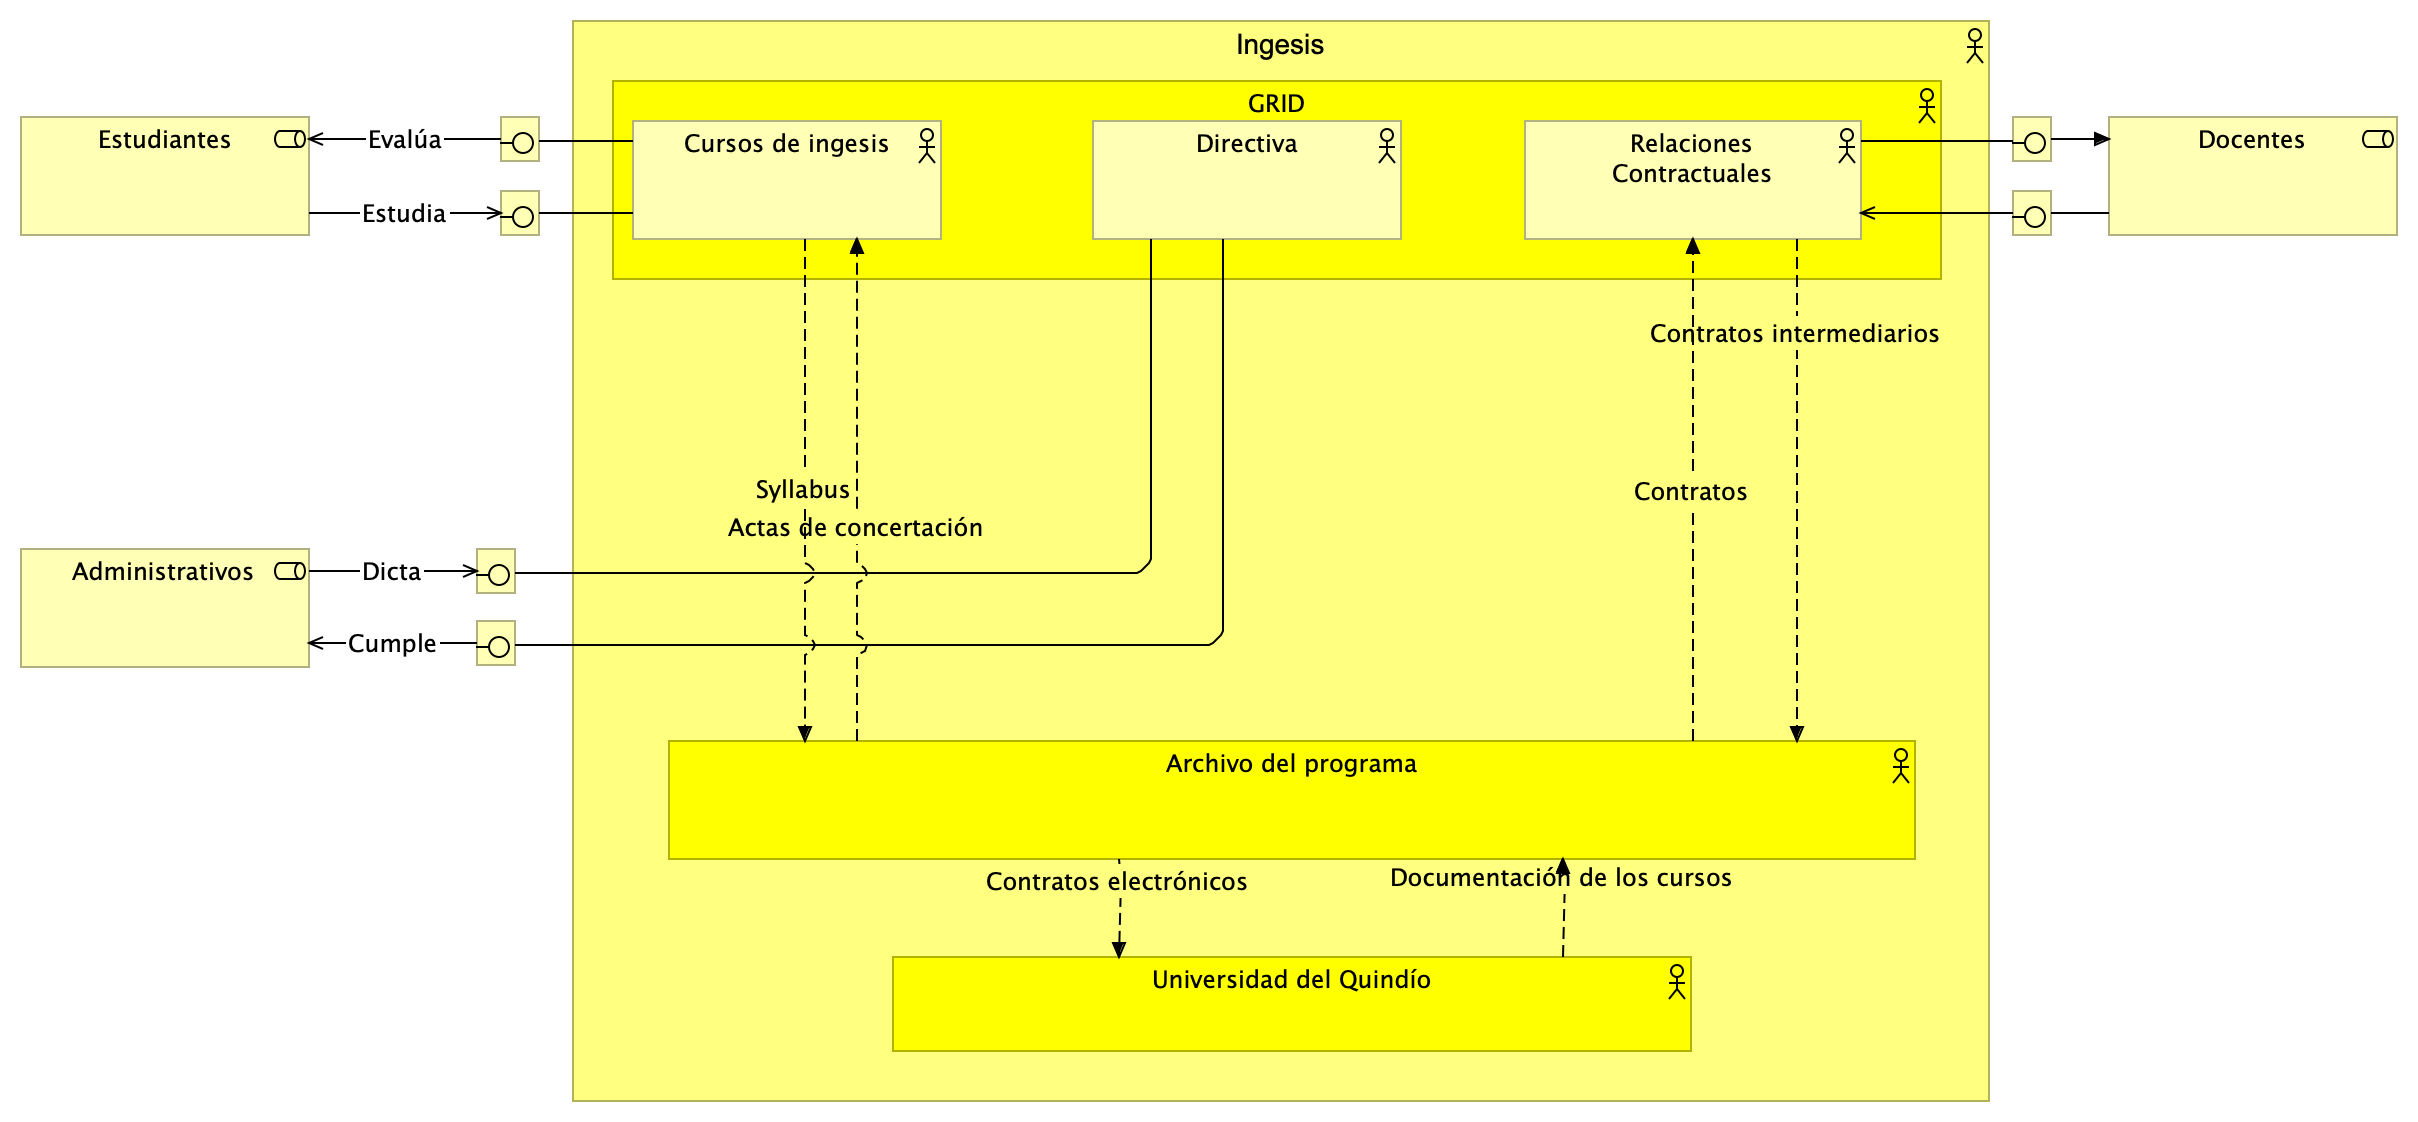
\includegraphics[width=\textwidth]{tablas-images/cp6/Actor-Cooperation-view.png}
    \caption{Vista de Cooperación de Actores}\label{fig:vista-cooperacion-actores}
\end{figure}

La figura~\ref{fig:vista-cooperacion-negocio} describe los procesos que permiten atender solicitudes de recursos tecnológicos, como contenedores, datasets o entornos virtualizados. Se observa cómo el investigador o grupo GRID registra una solicitud, pasa por validaciones, asignación de recursos (CPU, RAM, GPU, almacenamiento) y finalmente se despliega el contenedor. También se contempla la liberación de recursos cuando dejan de usarse. El diagrama integra servicios como autenticación, orquestación de contenedores y repositorios de imágenes, evidenciando cómo se coordinan los distintos procesos de negocio para garantizar disponibilidad y eficiencia en el uso de la infraestructura.

\begin{figure}[H]
    \centering
    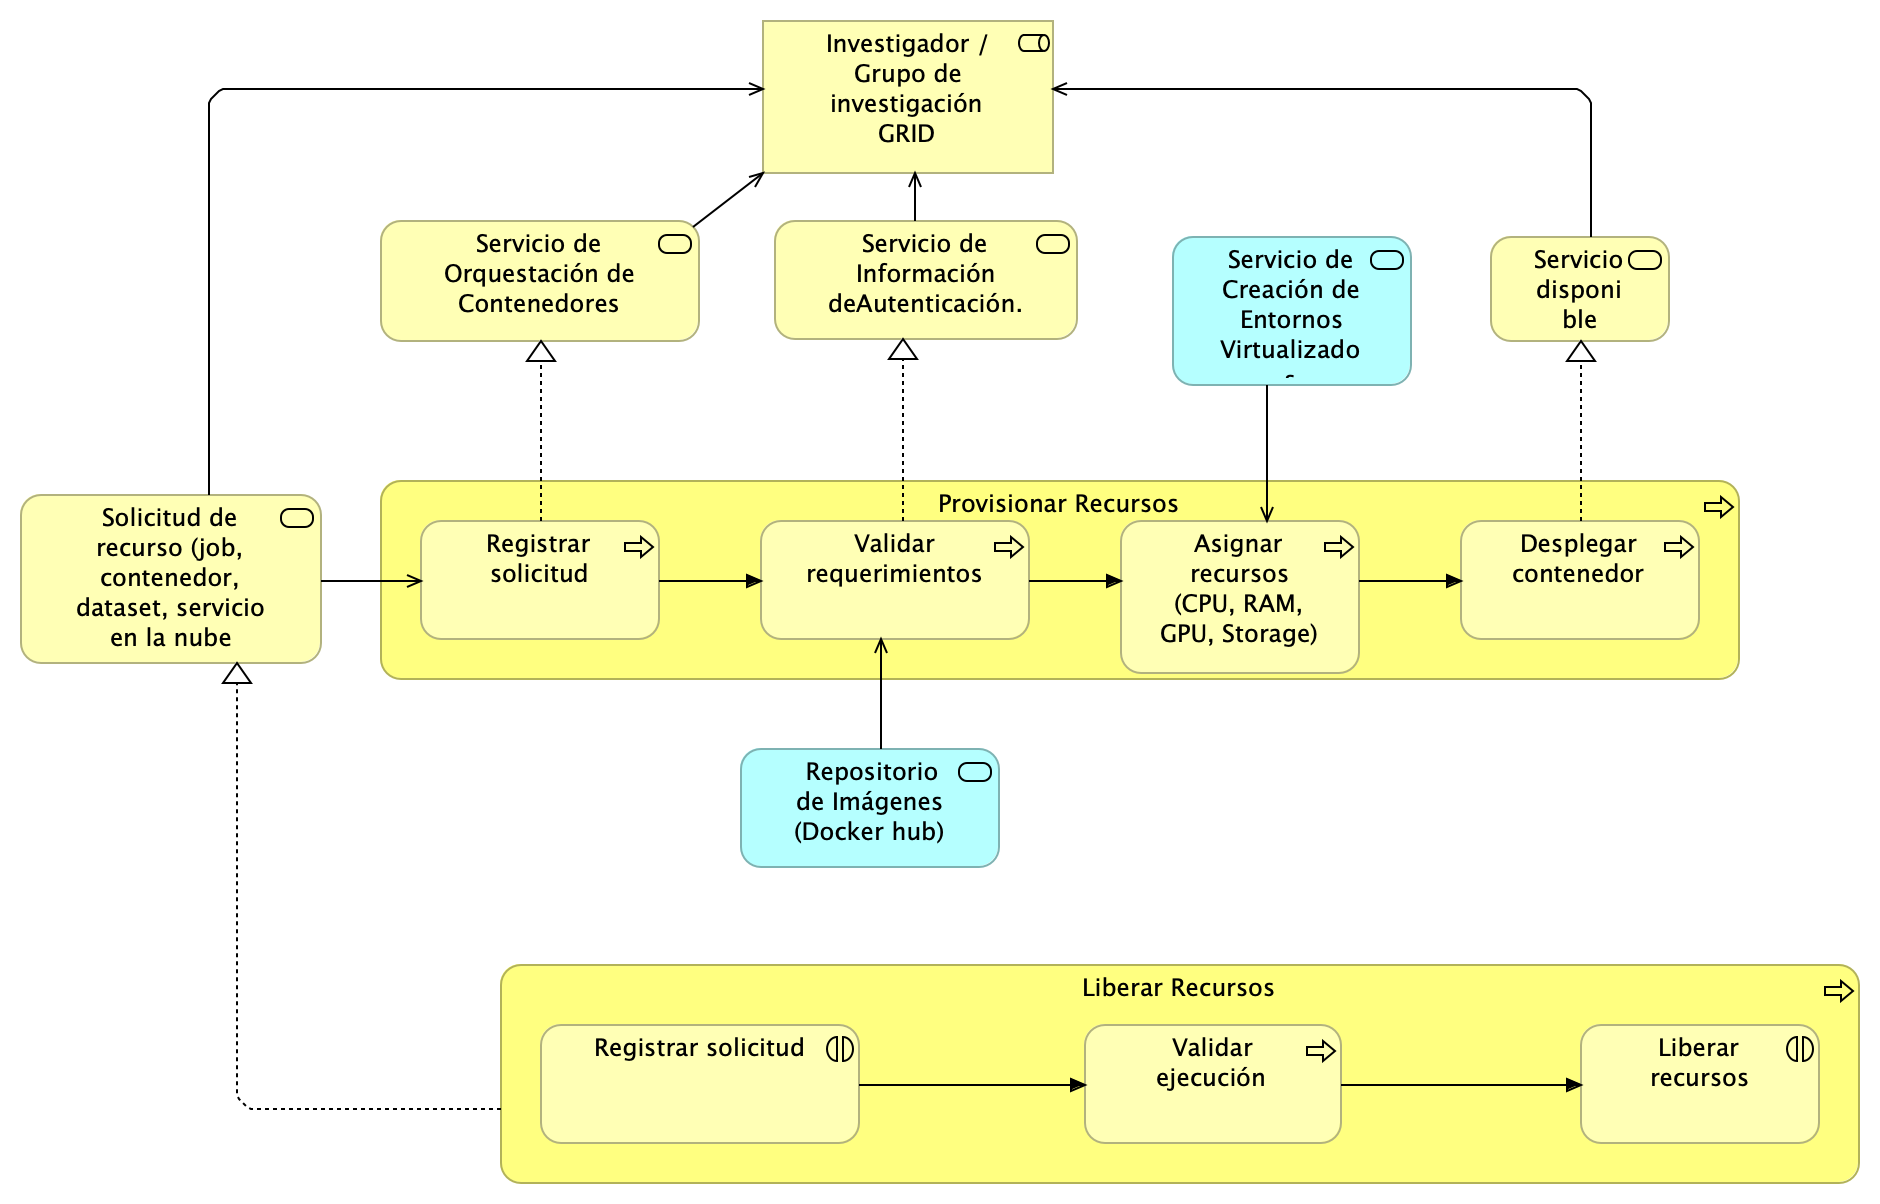
\includegraphics[width=\textwidth]{tablas-images/cp6/Business-Cooperation-View.png}
    \caption{Vista de Cooperación de Negocio}\label{fig:vista-cooperacion-negocio}
\end{figure}

El diagrama~\ref{fig:vista-productos-negocio} ilustra cómo los investigadores y estudiantes acceden a los recursos de cómputo bajo un marco regulado por políticas de uso y respaldado por un SLA. Muestra el flujo desde la solicitud hasta la ejecución de los contenedores, buscando la trazabilidad y control en el consumo de infraestructura.

\begin{figure}[H]
    \centering
    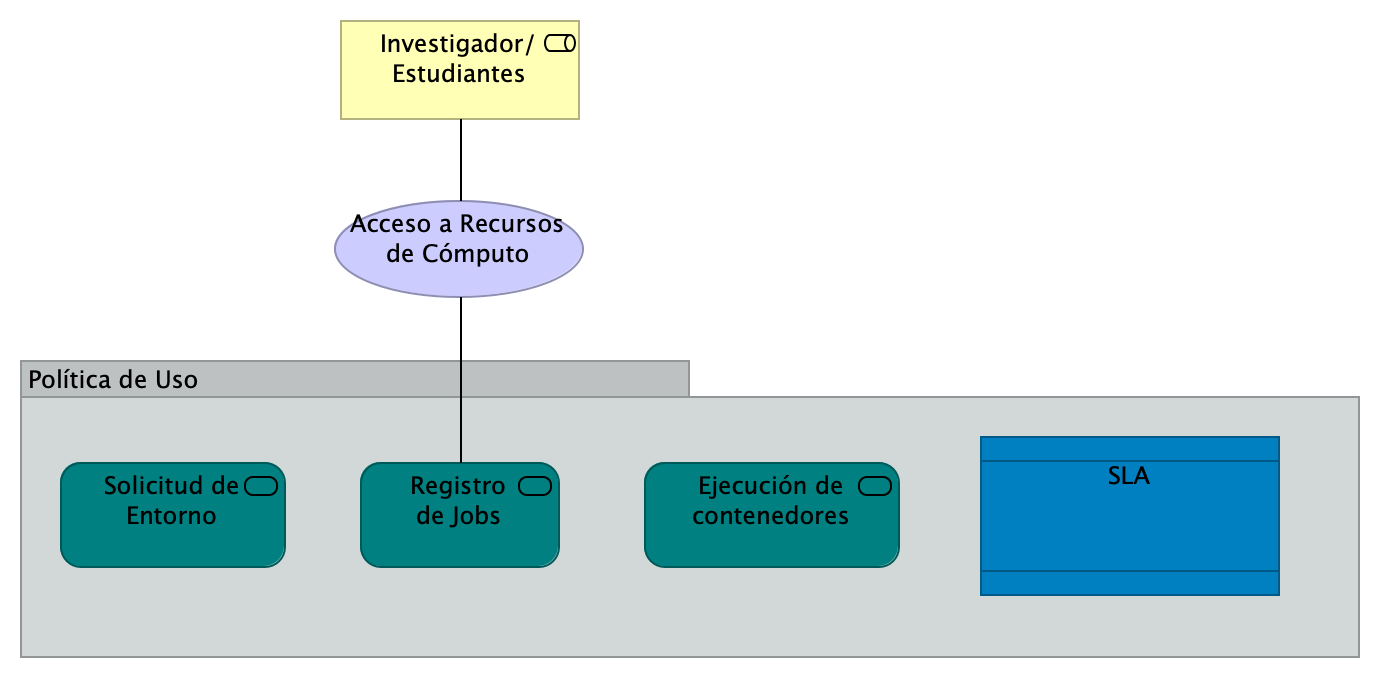
\includegraphics[width=\textwidth]{tablas-images/cp6/Business-Product-View.png}
    \caption{Vista de Producto de Negocio}\label{fig:vista-productos-negocio}
\end{figure}


La imagen~\ref{fig:vista-proceso-negocio} muestra el ciclo de vida completo de los entornos de cómputo: desde la solicitud de ejecución por parte de investigadores o estudiantes, pasando por el registro, validación, planificación de recursos y despliegue, hasta la liberación de los recursos una vez usados. En este flujo intervienen componentes clave como descriptores de jobs en Kubernetes, credenciales de clúster, registros de usuario, acuerdos de recursos, autenticación, orquestador y scheduler de prioridad. En conjunto, el modelo refleja cómo se gestionan de manera controlada y auditable los recursos computacionales dentro del sistema.
\begin{figure}[H]
    \centering
    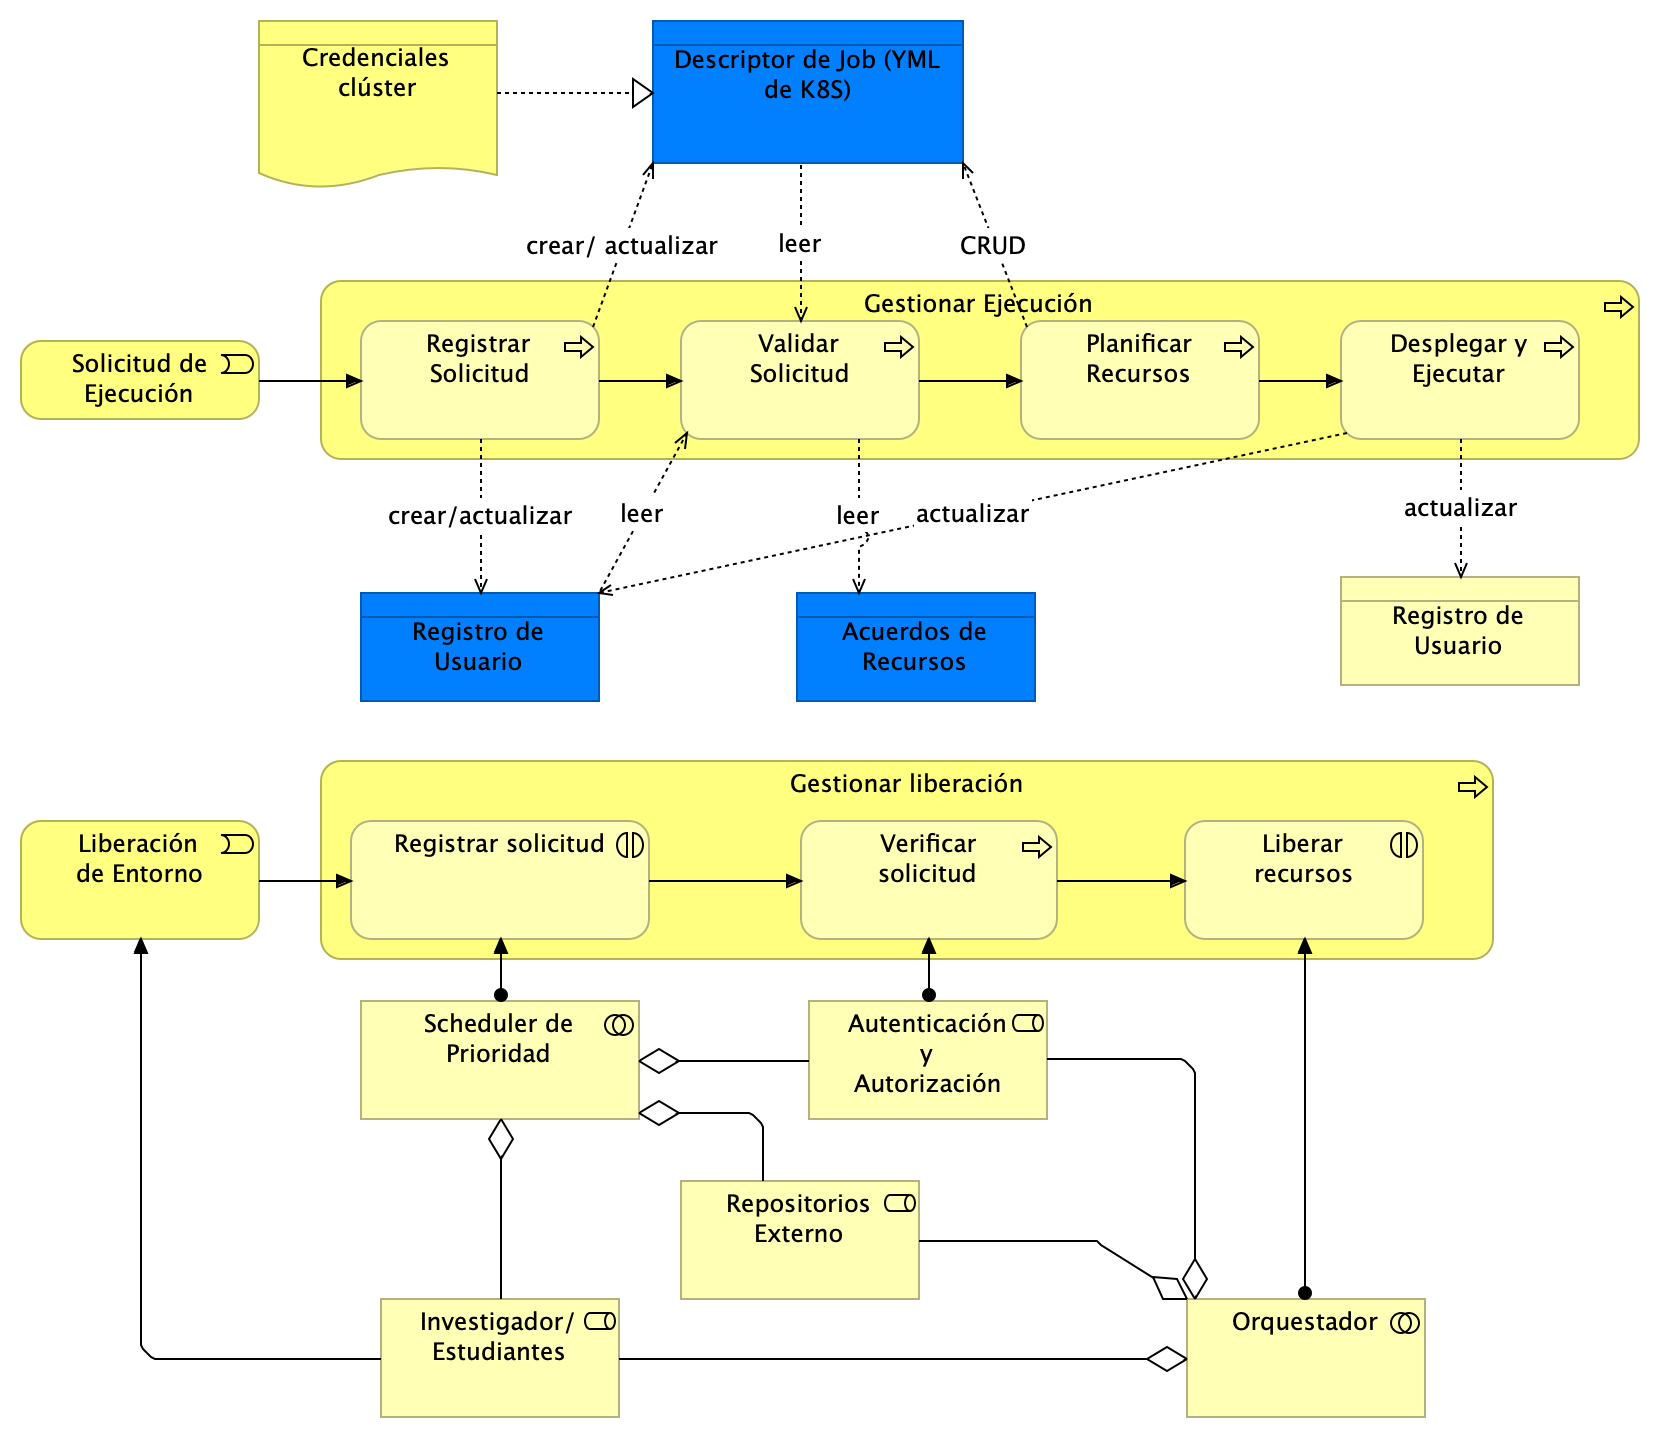
\includegraphics[width=\textwidth]{tablas-images/cp6/Business-Process-View.png}
    \caption{Vista de Proceso de Negocio}\label{fig:vista-proceso-negocio}
\end{figure}

El diagrama ~\ref{fig:vista-funcion-negocio}  muestra cómo la solución de virtualización basada en contenedores del GRID organiza sus principales funciones para dar soporte a estudiantes e investigadores. Entre ellas destacan la gestión de colaboraciones externas, la orquestación de recursos, la gestión de infraestructura virtualizada, la gestión de recursos de cómputo y consumo, la gestión de ejecuciones y la gestión de estudiantes e investigadores. El diagrama refleja la interacción entre actores clave (GRID, estudiantes/investigadores y datacenter Ingesis), señalando el flujo de información, el uso de infraestructura y los resultados de proyectos, lo que permite una administración integral  y alineada con los objetivos académicos y de investigación.

\begin{figure}[H]
    \centering
    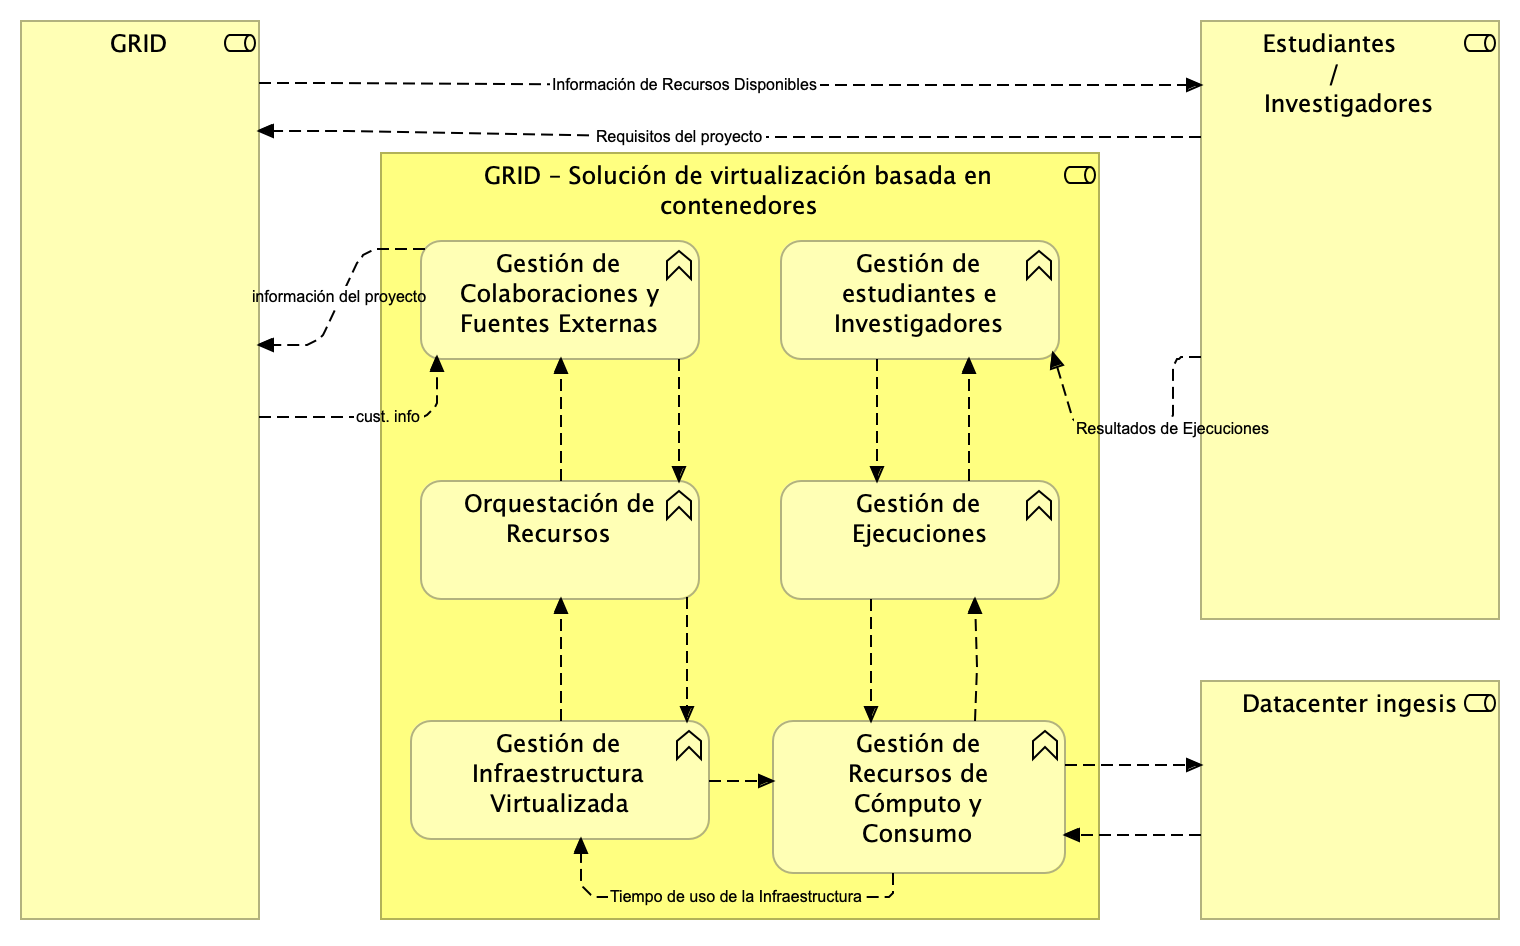
\includegraphics[width=\textwidth]{tablas-images/cp6/Business-Function-View.png}
    \caption{Vista de Función de Negocio}\label{fig:vista-funcion-negocio}
\end{figure}

\subsection{Vista de aplicación}
\begin{figure}[H]
    \centering
    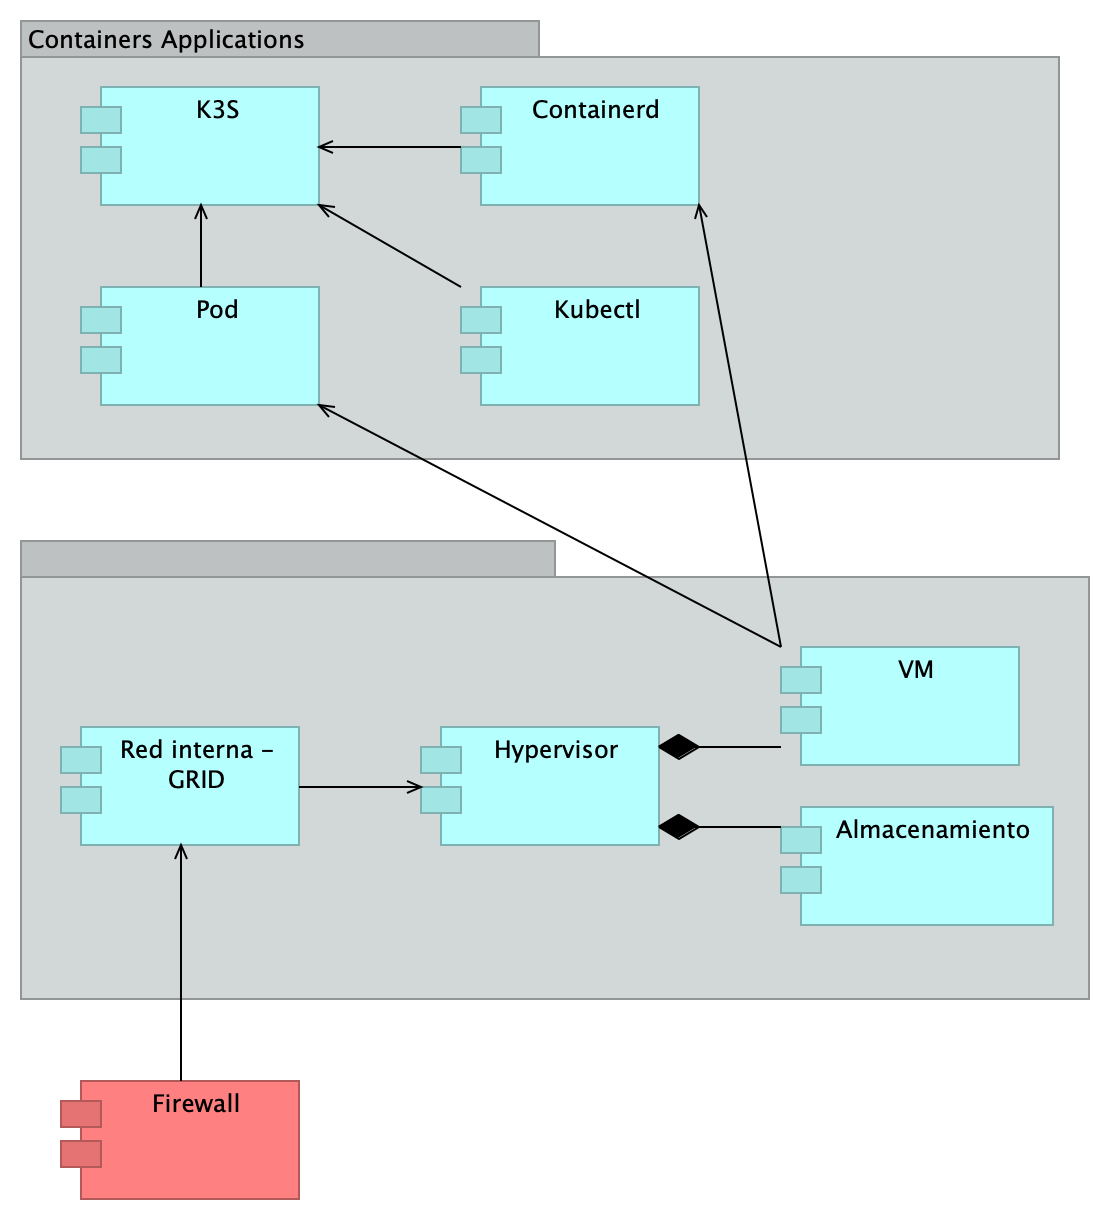
\includegraphics[width=\textwidth]{tablas-images/cp6/Application-Cooperation-View.png}
    \caption{Vista de Cooperación de Aplicaciones}
\end{figure}
\begin{figure}[H]
    \centering
    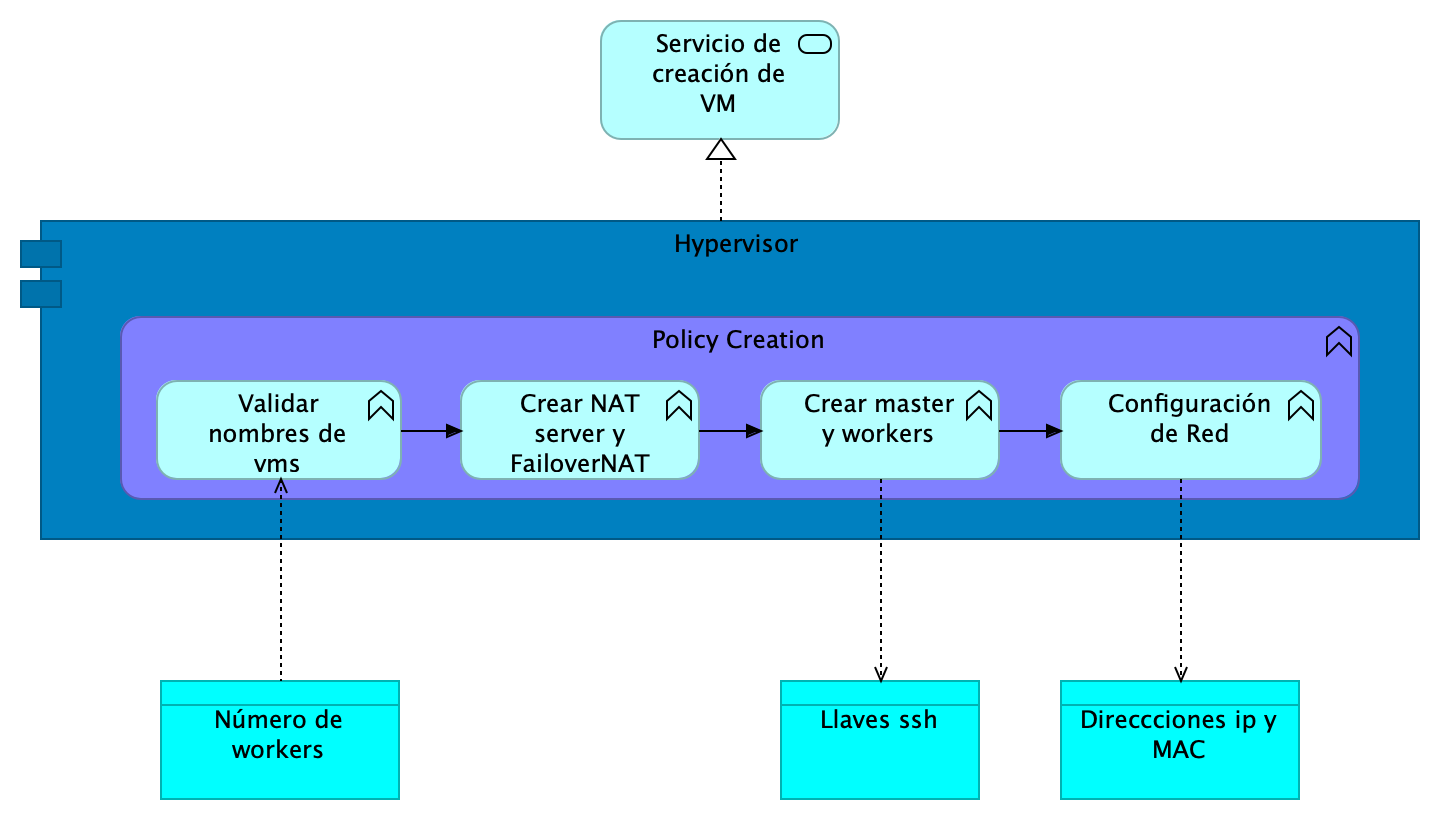
\includegraphics[width=\textwidth]{tablas-images/cp6/Application-Behaviour-view.png}
    \caption{Vista de Comportamiento de Aplicaciones}
\end{figure}
\begin{figure}[H]
    \centering
    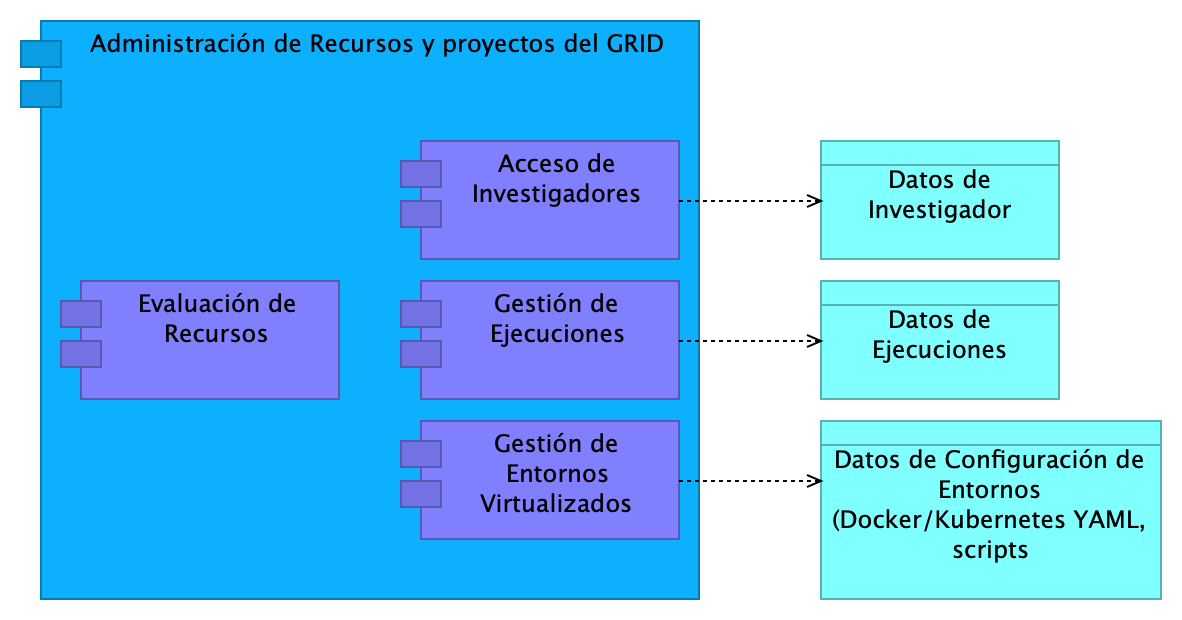
\includegraphics[width=\textwidth]{tablas-images/cp6/Application-Structure-View.png}
    \caption{Vista de Estructura de Aplicaciones}
\end{figure}

\subsection{Vista de tecnología}
\begin{figure}[H]
    \centering
    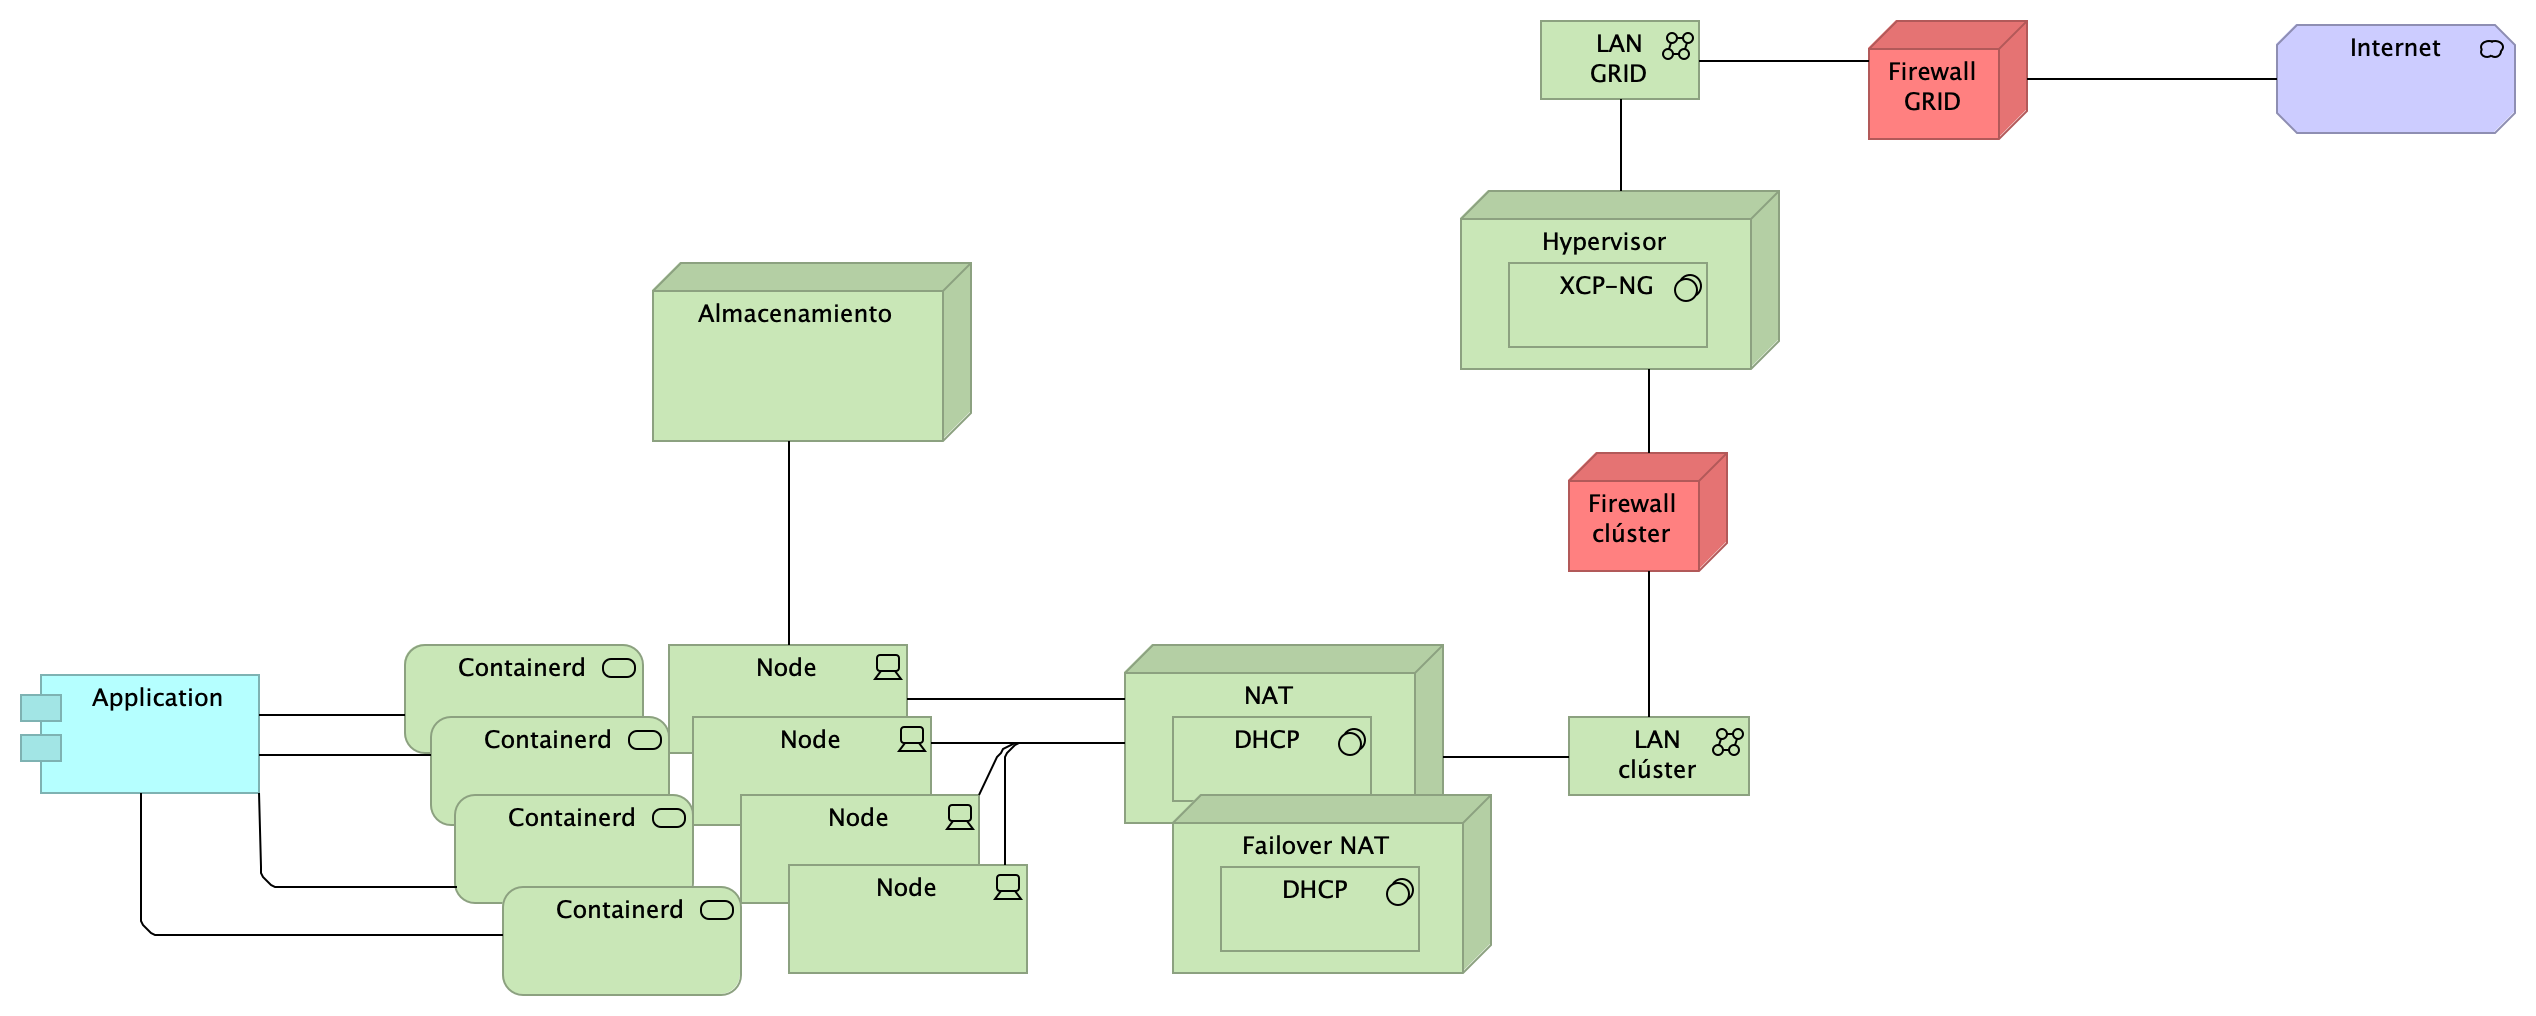
\includegraphics[width=\textwidth]{tablas-images/cp6/Implementation-and-Installation-View.png}
    \caption{Vista de Implementación e Instalación}
\end{figure}
\begin{figure}[H]
    \centering
    \includegraphics[width=\textwidth]{tablas-images/cp6/Information-Structure-View.png}
    \caption{Vista de Estructura de Información}
\end{figure}x


\subsection{Vista general}
% Vista general - Placeholder
% Este archivo contiene la vista general del modelo ArchiMate

\begin{figure}[H]
	\centering
	\includegraphics[width=\textwidth]{images/placeholder.png}
	\caption{Vista general del sistema}
	\label{fig:vista-general}
\end{figure}

% Descripción de la vista general
La vista general integra las tres capas del modelo ArchiMate (negocio, aplicación y tecnología) para proporcionar una perspectiva completa de la arquitectura de la solución. Esta vista permite visualizar las relaciones y dependencias entre los diferentes elementos del sistema HTCondor, desde los procesos de negocio hasta la infraestructura tecnológica que los soporta.

Esta vista consolidada facilita la comprensión del sistema en su totalidad y sirve como herramienta de comunicación entre los diferentes stakeholders del proyecto, permitiendo identificar puntos de integración críticos y oportunidades de optimización en toda la arquitectura.


\section{Diseño por capas de la solución}

\section{Capa de infraestructura}

\begin{figure}[H]
    \centering
    \includegraphics[width=\textwidth]{tablas-images/cp6/disenio-N1.png}
    \caption{Capa de Infraestructura}
\end{figure}

\section{Capa de virtualización}

\begin{figure}[H]
    \centering
    \includegraphics[width=\textwidth]{tablas-images/cp6/disenio-N2.png}
    \caption{Capa de Virtualización}
\end{figure}

\section{Capa de aplicación}

%
%\ChapterImageStar[cap:resultados]{Resultados}{./images/fondo.png}\label{cap:resultados}
\mbox{}\\
El desarrollo de esta investigación permitió obtener una serie de resultados tangibles y analíticos que responden a los objetivos planteados y contribuyen a la especificación de una solución arquitectónica basada en tecnologías de virtualización por contenedores (VBC) para el Grupo de Investigación en Redes, Información y Distribución (GRID) de la Universidad del Quindío. A continuación, se presentan los hallazgos más relevantes organizados según las fases metodológicas ejecutadas. En primer lugar, la caracterización del GRID permitió identificar sus capacidades tecnológicas actuales, su misión institucional y las necesidades específicas de sus stakeholders. Se determinó que el grupo cuenta con una infraestructura de virtualización basada en el hipervisor XCP-ng, compuesta por servidores tipo torre y rack, con especificaciones técnicas heterogéneas pero suficientes para soportar servicios educativos y de investigación. No obstante, se evidenció la necesidad de incorporar instancias computacionales más ligeras y eficientes que complementen la infraestructura existente y amplíen la oferta de servicios hacia la comunidad académica, en particular para los estudiantes de Ingeniería de Sistemas y Computación. El análisis de stakeholders permitió priorizar a los integrantes del GRID, docentes y estudiantes como actores clave, lo cual orientó el diseño de la solución hacia sus necesidades reales. La revisión sistemática de la literatura (SMS) arrojó como resultado la identificación y clasificación de 18 tecnologías VBC relevantes en el ámbito académico y profesional. Mediante una estrategia de búsqueda en bases de datos académicas y la técnica de bola de nieve, se seleccionaron y analizaron 116 estudios que permitieron construir un panorama actualizado del estado del arte. Tecnologías como Docker, Podman, LXC, Containerd, LXD, Singularity, Wasm, entre otras, fueron caracterizadas en términos de licencias, interfaces de uso, integración con nubes públicas, entornos de ejecución y adopción en la industria. La aplicación de un cuadrante Gartner permitió visualizar la posición relativa de cada tecnología, situando a Docker y Containerd en el cuadrante de líderes, mientras que otras como Udocker o Sarus se ubicaron como jugadores de nicho, orientados a entornos específicos como HPC. El benchmarking técnico realizado sobre un subconjunto de tecnologías preseleccionadas —Docker, Podman, LXC, LXD y Containerd— proporcionó mediciones objetivas de rendimiento en condiciones controladas. Los resultados mostraron diferencias significativas en el consumo de recursos, tiempo de arranque, throughput de red y latencia de E/S. Containerd destacó por su eficiencia general, con un bajo consumo de CPU (99.71\% de tiempo en idle), un tiempo de arranque rápido y una latencia de disco reducida. LXC, por su parte, mostró el menor consumo de memoria RAM (2.835\%) y el mejor desempeño en throughput de red, aunque con un tiempo de arranque superior. Podman, si bien eficiente en recursos, presentó limitaciones en el rendimiento de red y E/S. Estos resultados proporcionaron una base cuantitativa para la toma de decisiones subsiguiente. El Análisis de Decisiones y Resolución (DAR), aplicado conforme al modelo CMMI, permitió evaluar las tecnologías VBC con base en 12 criterios técnicos y organizacionales, entre los que se incluyeron: tipo de licencia, posibilidad de orquestación, compatibilidad con Docker Hub, soporte para redes personalizadas, persistencia de datos, documentación, soporte comunitario, popularidad, consumo de recursos, compatibilidad con orquestadores y costos de implementación. Containerd obtuvo la puntuación más alta (233/300), destacando por su licencia Apache 2.0, integración nativa con Kubernetes, amplia documentación, bajo consumo de recursos y compatibilidad total con el ecosistema Docker. Adicionalmente, se evaluaron distintas alternativas de motores de orquestación para Kubernetes, donde K3S resultó seleccionado por su facilidad de instalación, bajo consumo de recursos y compatibilidad con entornos limitados en hardware. Con base en lo anterior, se diseñó una solución arquitectónica modelada en Archimate, que integra la infraestructura existente del GRID con una capa de virtualización basada en Containerd y K3S. El modelo incluye vistas de negocio, aplicación y tecnología, articulando procesos como la solicitud de entornos virtualizados, la provisión de recursos y la gestión de ejecuciones. Se propuso un modelo por capas que separa claramente la infraestructura física, la capa de virtualización (contenedores y orquestación) y la capa de aplicación, facilitando así el mantenimiento, la escalabilidad y la gestión de servicios. Finalmente, se implementó y validó un producto mínimo viable (PMV) que materializó la arquitectura propuesta. El PMV fue desplegado en un entorno controlado dentro de la infraestructura del GRID, permitiendo la ejecución de contenedores OCI gestionados mediante K3S y Containerd. La validación incluyó pruebas de funcionalidad, rendimiento y usabilidad, realizadas en colaboración con usuarios potenciales (investigadores y estudiantes). Los resultados de estas pruebas confirmaron que la solución es estable, reproducible y adecuada para su uso en escenarios académicos y de investigación, cumpliendo con los requerimientos identificados durante la caracterización inicial. En conjunto, estos resultados demuestran que la incorporación de Containerd y K3S en la infraestructura del GRID representa una alternativa viable y eficiente para expandir su portafolio de servicios mediante contenedores, sin desestimar la inversión previa en virtualización tradicional. La metodología aplicada —que combinó caracterización contextual, revisión sistemática, evaluación técnica y diseño arquitectónico— provee un marco reproducible para la selección e implementación de tecnologías VBC en contextos académicos con restricciones de recursos y alineados con misiones institucionales de docencia, investigación y extensión.
%\ChapterImageStar[cap:conclusiones]{Conclusiones}{./images/fondo.png}\label{cap:conclusiones}
\mbox{}\\
%\ChapterImageStar[cap:trabajos-futuros]{Trabajos Futuros}{./images/fondo.png}\label{cap:trabajos-futuros}
\mbox{}\\
%
%\ChapterImageStar[cap:cumplimiento-objetivos]{Cumplimiento de objetivos}{./images/fondo.png}\label{cap:cumplimiento-objetivos}



% Referencias - con imagen de fondo específica
\cleardoublepage\thispagestyle{empty}
\refstepcounter{chapter}
\phantomsection\addcontentsline{toc}{chapter}{Referencias}\label{cap:referencias}

% Imagen de fondo específica para referencias
\AddToShipoutPicture*{%
	\put(0,0){\includegraphics[width=\paperwidth,height=\paperheight]{./images/referencias.png}}%
}

% Título posicionado con coordenadas absolutas (en píxeles desde esquina superior izquierda)
\begin{tikzpicture}[remember picture,overlay]
	\node[anchor=north west] at ([xshift=150pt,yshift=-370pt]current page.north west)
	{\Large\bfseries\textcolor{black}{Referencias}};
\end{tikzpicture}
\vspace{2cm}

% Bibliografía sin título automático
\begingroup
\renewcommand{\bibname}{}
\pagestyle{fancy} % Fuerza el estilo fancy para todas las páginas de bibliografía
\bibliographystyle{apalike}
\bibliography{bibliografia}
\endgroup

\appendix

% CHAPTER Búsquedas en bases de datos

\phantomsection

% Increment the chapter counter so \thechapter shows the correct number
% and make it referenceable with \ref
\refstepcounter{chapter}

% Manually add this appendix to the Table of Contents
\addcontentsline{toc}{chapter}{Apéndice \thechapter: Búsqueda en bases de datos}

% Add vertical space above the title (mimics standard chapter spacing)
\vspace{40pt}

% Display the actual chapter title (centered, large, bold)
{\centering \normalfont\huge\bfseries Apéndice~\thechapter: Búsqueda en bases de datos~\par}

% Add spacing between title and horizontal rule
\vspace{10pt}

% Draw a horizontal line across the page for visual separation
{\centering \rule{\textwidth}{0.4pt} \par}

% Add vertical space between title section and content
\vspace{40pt}

% Set the running headers for left and right pages
\markboth{Apéndice \thechapter:Búsqueda en bases de datos}{Apéndice \thechapter: Búsqueda en bases de datos}



\FloatBarrier\section{Cadenas de búsqueda}\label{sec:cadenas-busqueda}


\begin{tcolorbox}[
		colback=gray!5,
		colframe=black!60,
		title=Cadena de búsqueda en ACM Full Text Collection,
		fonttitle=\bfseries,
		sharp corners=south
	]
	\scriptsize
	\begin{verbatim}
((HTCondor OR Condor) AND (HTC OR "High Throughput Computing" OR HPC OR "High
Performance Computing") AND (Universe OR "Execution Environment") AND (Project OR
Work) AND (Research OR Teaching OR Industry))
	\end{verbatim}
\end{tcolorbox}

\begin{tcolorbox}[
		colback=gray!5,
		colframe=black!60,
		title=Cadena de búsqueda en IEEE Xplore,
		fonttitle=\bfseries,
		sharp corners=south
	]
	\scriptsize
	\begin{verbatim}
(HTCondor OR Condor) AND (HTC OR (High Throughput Computing)) AND (Universe OR
(Runtime Environment)) AND (Research OR Teaching OR Industry)
	\end{verbatim}
\end{tcolorbox}

\begin{tcolorbox}[
		colback=gray!5,
		colframe=black!60,
		title=Cadena de búsqueda en Springer,
		fonttitle=\bfseries,
		sharp corners=south
	]
	\scriptsize
	\begin{verbatim}
((HTCondor — Condor) + (HTC — "High Throughput Computing" — HPC — "High
Performance Computing") + (Universe — "Execution Environment") + (Project — Work) +
(Research — Teaching — Industry))
	\end{verbatim}
\end{tcolorbox}

\begin{tcolorbox}[
		colback=gray!5,
		colframe=black!60,
		title=Cadena de búsqueda en ScienceDirect,
		fonttitle=\bfseries,
		sharp corners=south
	]
	\scriptsize
	\begin{verbatim}
(HTCondor OR Condor) (HTC OR "High Throughput Computing" OR HPC OR "High Performance Computing") (Universe OR "Execution Environment") (Project OR Work) (Research OR
Teaching OR Industry)
	\end{verbatim}
\end{tcolorbox}

\begin{tcolorbox}[
		colback=gray!5,
		colframe=black!60,
		title=Cadena de búsqueda en Taylor \& Francis,
		fonttitle=\bfseries,
		sharp corners=south
	]
	\scriptsize
	\begin{verbatim}
(HTCondor OR Condor) AND (HTC OR (High Throughput Computing)) AND (Universe OR
(Runtime Environment)) AND (Research OR Teaching OR Industry)
  \end{verbatim}
\end{tcolorbox}


\section{Búsqueda de artículos sin criterios de inclusión/exclusión}\label{sec:busqueda-sin-criterios}

% ##### Imagenes de busqueda ########

\begin{figure}[H]
	\centering
	\includegraphics[width=\textwidth,keepaspectratio]{apendices/bases-datos/sin-exclusion/acm.png}
	\caption{Búsqueda de artículos de educación en ACM sin criterios de inclusión/exclusión \\
		Fecha de acceso: 12/03/25 9:13 pm
	}\label{fig:busqueda-acm-no-exclusion}
\end{figure}

\FloatBarrier

\begin{figure}[H]
	\centering
	\includegraphics[width=\textwidth,keepaspectratio]{apendices/bases-datos/sin-exclusion/science-direct.png}
	\caption{Búsqueda de artículos de investigación en ACM sin criterios de inclusión/exclusión \\
		Fecha de acceso: 12/03/25 8:23 pm
	}\label{fig:busqueda-science-direct-no-exclusion}
\end{figure}

\begin{figure}[H]
	\centering
	\includegraphics[width=\textwidth,keepaspectratio]{apendices/bases-datos/sin-exclusion/springer.png}
	\caption{Búsqueda de artículos de investigación en ACM sin criterios de inclusión/exclusión \\
		Fecha de acceso: 12/03/25 8:23 pm
	}\label{fig:busqueda-springer-no-exclusion}
\end{figure}


%########## Fin Imagenes %###################


\section{Búsqueda de artículos con criterios de inclusión/exclusión}\label{sec:busqueda-con-criterios}

\begin{figure}[H]
	\centering
	\includegraphics[width=\textwidth,keepaspectratio]{apendices/bases-datos/con-exclusion/acm.png}
	\caption{Búsqueda de artículos de educación en ACM sin criterios de inclusión/exclusión \\
		Fecha de acceso: 12/03/25 9:13 pm
	}\label{fig:busqueda-acm-con-exclusion}
\end{figure}

\FloatBarrier

\begin{figure}[H]
	\centering
	\includegraphics[width=\textwidth,keepaspectratio]{apendices/bases-datos/con-exclusion/science-direct.png}
	\caption{Búsqueda de artículos de investigación en ACM sin criterios de inclusión/exclusión \\
		Fecha de acceso: 12/03/25 8:23 pm
	}\label{fig:busqueda-science-direct-con-exclusion}
\end{figure}

\begin{figure}[H]
	\centering
	\includegraphics[width=\textwidth,keepaspectratio]{apendices/bases-datos/con-exclusion/springer.png}
	\caption{Búsqueda de artículos de investigación en ACM sin criterios de inclusión/exclusión \\
		Fecha de acceso: 12/03/25 8:23 pm
	}\label{fig:busqueda-springer-con-exclusion}
\end{figure}

\newpage



% CHAPTER Implementación del univeso Parallel
\phantomsection

% Increment the chapter counter so \thechapter shows the correct number
% and make it referenceable with \ref
\refstepcounter{chapter}

% Manually add this appendix to the Table of Contents
\addcontentsline{toc}{chapter}{Apéndice \thechapter: Implementación del clúster virtualizado HTCondor}

% Add vertical space above the title (mimics standard chapter spacing)
\vspace{40pt}

% Display the actual chapter title (centered, large, bold)
{\centering \normalfont\huge\bfseries Apéndice~\thechapter: Implementación del clúster virtualizado HTCondor~\par}

% Add spacing between title and horizontal rule
\vspace{10pt}

% Draw a horizontal line across the page for visual separation
{\centering \rule{\textwidth}{0.4pt} \par}

% Add vertical space between title section and content
\vspace{40pt}

% Set the running headers for left and right pages
\markboth{Apéndice \thechapter: Implementación del clúster virtualizado HTCondor}{Apéndice \thechapter: Implementación del clúster virtualizado HTCondor}


\FloatBarrier\subsection{Instalación en un entorno virtualizado}

El clúster de computación distribuida de HTCondor actualmente soporta la versión \texttt{8.4.11}. A continuación se muestra la salida de uno de los nodos Raspberry-Pi, los cuales tienen una instalación heterogénea:

% HTCondor version output
\begin{minted}[
    frame=lines,
    framesep=2mm,
    baselinestretch=1.2,
    bgcolor=lightgray!10,
    fontsize=\footnotesize,
]{bash}
condor_version
$CondorVersion: 8.4.11 Feb 06 2017 BuildID: Debian-8.4.11~dfsg.1-1 Debian-8.4.11~dfsg.1-1
$$CondorPlatform: ARMV7L-Raspbian_ $
\end{minted}


Si bien esta versión es compatible con el \textbf{universo parallel}, la limitada documentación disponible para la version \texttt{8.4.11} en particular representó un obstáculo para implementar algoritmos que utilizaran OpenMPI. Por esta razón, y siguiendo la recomendación del asesor de este proyecto, se decidió implementar dicho universo en una infraestructura virtualizada.

\FloatBarrier\subsubsection{Infraestrutura virtualizada}

El primer paso hacia la implementación de la nueva infraestructura HTCondor fue desplegar máquinas virtuales en la infraestructura del \GRID. Para ello se utilizó un servidor dedicado que ejecuta el hipervisor \cite{xcpng_intro}, en el cual se configuraron 5 máquinas virtuales con el sistema operativo~\texttt{AlmaLinux 9.6 (Sage Margay) x86\_64}. Las máquinas pueden verse, mediante la interfaz Xen-Orchestra en la figura \ref{fig:xen-vms}. Esta configuración difiere significativamente de la arquitectura armv7l de 32 bits que utiliza el clúster de Raspberry Pi actual. La elección de este sistema operativo no fue trivial, se fundamentó en varios criterios: según la documentación oficial, AlmaLinux es uno de los sistemas operativos oficialmente soportados por HTCondor~\cite{HTCondor_install}, además de haber sido implementado exitosamente por instituciones como el CERN \citep{Bunsic2025}.

\begin{figure}
	\centering
	\includegraphics[scale=0.25]{apendices/infra-virtual/xen-vms.png}
	\caption{Vista de las máquinas virtuales para la nueva infraestructura HTCondor virtualizada de \GRID}
	\label{fig:xen-vms}
\end{figure}

A cada máquina se le asignó, al momento de instalación, una dirección IP dentro de la red \texttt{172.30.28.0/24} como se muestra en la Tabla~\ref{tab:nodos-htcondor}:

\begin{table}[H]
	\centering
	\renewcommand{\arraystretch}{1.2} % Espaciado reducido
	\fontsize{9pt}{10pt}\selectfont % Tamaño de fuente 9pt
	\begin{tabular}{|p{3cm}|p{3cm}|p{4.5cm}|p{2.5cm}|}  % Total: 14cm (incluyendo bordes)
		\hline
		\textbf{Rol del nodo} & \textbf{Dirección IP} & \textbf{Nombre de usuario} & \textbf{Usuario} \\ \hline
		Grid Manager          & 172.30.28.29          & gridmanager                & alma             \\ \hline
		Master                & 172.30.28.30          & master                     & alma             \\ \hline
		Submit                & 172.30.28.31          & submit                     & alma             \\ \hline
		Ejecutor 1            & 172.30.28.32          & exec01                     & alma             \\ \hline
		Ejecutor 2            & 172.30.28.33          & exec02                     & alma             \\ \hline
		Ejecutor 3            & 172.30.28.34          & exec03                     & alma             \\ \hline
	\end{tabular}
	\caption{Configuración de nodos del clúster HTCondor virtualizado}
	\label{tab:nodos-htcondor}
\end{table}


\FloatBarrier\subsubsection{Instalación de HTCondor}

Para la instalación de HTCondor se diseño el siguiente script, el cual emplea otro script que puede encontrarse en la documentación oficial \cite{HTCondor-linux-install}.



% HTCondor Install script
\begin{minted}[
    frame=lines,
    framesep=2mm,
    baselinestretch=1.2,
    bgcolor=lightgray!10,
    fontsize=\footnotesize,
]{bash}
#!/bin/bash

# Script de instalación de HTCondor para Alma Linux 9.6
# Uso: ./install-condor.sh <tipo_nodo> <hostname_master> <contraseña>
# Tipos de nodo: master, submit, worker

if [ "$#" -ne 3 ]; then
    echo "Uso: $0 <tipo_nodo> <hostname_master> <contraseña>"
    echo "Tipos de nodo: master, submit, worker"
    echo "Ejemplo: $0 master master.example.com micontraseña"
    exit 1
fi

NODE_TYPE=$1 #Tipo de nodo, hay tres opciones: {'master', 'submit' y 'worker;}
MASTER_FQN=$2 # Fully Qualified Name del nodo maestro.
PASSWORD=$3 #Deberá ser igual para todos los nodos de manera que puedan comunicarse entre sí

sudo dnf update -y

case $NODE_TYPE in
    master)
        echo "Instalando nodo MASTER..."
        curl -fsSL https://get.htcondor.org | sudo /bin/bash -s -- --no-dry-run --cm $MASTER_FQN --password $PASSWORD --channel lts
        ;;
    submit)
        echo "Instalando nodo SUBMIT (access point)..."
        curl -fsSL https://get.htcondor.org | sudo /bin/bash -s -- --no-dry-run --ap $MASTER_FQN --password $PASSWORD --channel lts
        ;;
    worker)
        echo "Instalando nodo WORKER (execution point)..."
        curl -fsSL https://get.htcondor.org | sudo /bin/bash -s -- --no-dry-run --ep $MASTER_FQN --password $PASSWORD --channel lts
        ;;
    *)
        echo "Error: Tipo de nodo inválido. Use: master, submit o worker"
        exit 1
        ;;
esac

echo "Instalación completada exitosamente!"
\end{minted}


Aparte del script anterior, también se creó una guía en formato .md la cual puede ser encontrada en el siguiente \href{https://github.com/Parritap/HTcondor/blob/master/alma-linux-cluster/README-ES.md}{https://github.com/Parritap/HTcondor/blob/master/alma-linux-cluster/README-ES.md}.



Para HTcondor es muy importante que los nodos puedan comunicarse entre sí, para lograr esto, se editaron los archivos \texttt{/etc/hosts} en cada uno de los nodos. Dicha edición puede verse en a continuación:

% HTCondor Install script
\begin{minted}[
    frame=lines,
    framesep=2mm,
    baselinestretch=1.2,
    bgcolor=lightgray!10,
    fontsize=\footnotesize,
]{bash}
#Parallel config
172.30.28.30 master
172.30.28.31 submit
172.30.28.32 exec01
172.30.28.33 exec02
172.30.28.34 exec03
172.30.28.35 exec04
\end{minted}

Después de dicha configuración podremos ejecutar el comando \texttt{condor\_status} y ver lo siguiente impreso en consola:

\begin{minted}[
    frame=lines,
    framesep=2mm,
    baselinestretch=1.2,
    bgcolor=lightgray!10,
    fontsize=\footnotesize,
]{bash}
Name         OpSys      Arch   State     Activity LoadAv Mem   ActvtyTime

slot1@exec01 LINUX      X86_64 Unclaimed Idle      0.000 1763  6+02:39:58
slot1@exec02 LINUX      X86_64 Unclaimed Idle      0.000 1763  6+02:34:51
slot1@exec03 LINUX      X86_64 Unclaimed Idle      0.000 1763  6+02:34:43

               Total Owner Claimed Unclaimed Matched Preempting  Drain Backfill BkIdle

  X86_64/LINUX     3     0       0         3       0          0      0        0      0

         Total     3     0       0         3       0          0      0        0      0

\end{minted}

%!TODO
\FloatBarrier\subsection{Instalación de un implementación \MPI}

Para permitir la comunicación entre trabajos distribuidos fuertemente acoplados en un pool HTCondor, es necesario implementar una tecnología basada en el estándar~\MPI. En este contexto, se seleccionó OpenMPI debido a que, según la documentación oficial de HTCondor \cite{HTCondor_Parallel}, esta implementación particular del estándar MPI cuenta con soporte nativo, lo que facilita su integración con el sistema de gestión de trabajos. El script de instalación de OpenMPI para el sistema operativo Alma Linux se presenta a continuación:

% HTCondor Install script
\begin{minted}[
    frame=lines,
    framesep=2mm,
    baselinestretch=1.2,
    bgcolor=lightgray!10,
    fontsize=\footnotesize,
]{bash}
sudo dnf update -y
sudo dnf install openmpi openmpi-devel -y

echo "module load mpi/openmpi-x86_64" >> ~/.bashrc
source ~/.bashrc
\end{minted}

\newpage


% CHAPTER Implementación del univeso Parallel
\phantomsection

% Increment the chapter counter so \thechapter shows the correct number
% and make it referenceable with \ref
\refstepcounter{chapter}

% Manually add this appendix to the Table of Contents
\addcontentsline{toc}{chapter}{Apéndice \thechapter: Configuración del universo Grid en la infraestructura HTCondor del Grupo GRID}

% Add vertical space above the title (mimics standard chapter spacing)
\vspace{40pt}

% Display the actual chapter title (centered, large, bold)
{\centering \normalfont\huge\bfseries Apéndice~\thechapter: Configuración del universo Grid en la infraestructura HTCondor del Grupo GRID~\par}

% Add spacing between title and horizontal rule
\vspace{10pt}

% Draw a horizontal line across the page for visual separation
{\centering \rule{\textwidth}{0.4pt} \par}

% Add vertical space between title section and content
\vspace{40pt}

% Set the running headers for left and right pages
\markboth{Apéndice \thechapter: Configuración del universo Grid}{Apéndice \thechapter: Configuración del universo Grid}

\FloatBarrier\subsection{Configuración del universo Grid}

El universo Grid de HTCondor permite la ejecución de trabajos a través de múltiples clústeres distribuidos geográficamente, facilitando el aprovechamiento de recursos computacionales heterogéneos. La infraestructura del Grupo \GRID implementa este universo mediante un nodo coordinador (\textit{grid manager}) que gestiona la distribución de trabajos hacia clústeres remotos con el universo Vanilla.

La configuración actual soporta la versión \texttt{8.4.11} de HTCondor en arquitectura \texttt{armv7l} sobre sistema operativo Raspbian GNU/Linux 9 (stretch). A continuación se muestra la salida del comando de versión en el nodo \textit{grid manager}:

% HTCondor version output
\begin{minted}[
    frame=lines,
    framesep=2mm,
    baselinestretch=1.2,
    bgcolor=lightgray!10,
    fontsize=\footnotesize,
]{bash}
$CondorVersion: 8.4.11 Feb 06 2017 BuildID: Debian-8.4.11~dfsg.1-1 Debian-8.4.11~dfsg.1-1 $
$CondorPlatform: ARMV7L-Raspbian_ $
\end{minted}

\FloatBarrier\subsubsection{Arquitectura del universo Grid}

El universo Grid en la infraestructura del Grupo~\GRID implementa una arquitectura federada donde un nodo coordinador central gestiona la distribución de trabajos hacia múltiples clústeres Vanilla independientes. Esta arquitectura permite la utilización de recursos distribuidos y proporciona tolerancia a fallos mediante la capacidad de redirigir trabajos entre diferentes clústeres.

\textbf{Componentes principales:}

\begin{itemize}
	\item \textbf{grid manager (172.30.27.11)}: Nodo coordinador que ejecuta los \textit{daemons} \texttt{SCHEDD}, \texttt{MASTER}, \texttt{GRIDMANAGER} y \texttt{COLLECTOR}, responsable de recibir trabajos desde la aplicación \textit{Grid App} y distribuirlos hacia los clústeres Vanilla disponibles.
	
	\item \textbf{Clúster Vanilla B}: Infraestructura computacional compuesta por un \textit{master/central manager} (172.30.27.34), un nodo \textit{submit} (172.30.27.35) y múltiples nodos \textit{Execute} (172.30.27.36-48).

	\item \textbf{Clúster Vanilla C}: Segunda infraestructura computacional con \textit{master/central manager} (172.30.27.66), nodo \textit{submit} (172.30.27.67) y nodos \textit{Execute} (172.30.27.68-80).
\end{itemize}

\begin{figure}
	\centering
	\includegraphics[scale=0.11]{apendices/infra-virtual/Diagramas HTCondor-Grid-flow.drawio.png}
	\caption{Arquitectura del universo Grid en la infraestructura HTCondor del~\GRID}
	\label{fig:grid-architecture}
\end{figure}

\FloatBarrier\subsubsection{Configuración del \textit{grid manager}}

El \textit{grid manager} constituye el componente central del universo Grid, implementando la lógica de distribución de trabajos y coordinación con clústeres remotos. Su configuración se basa en el archivo \texttt{/etc/condor/condor\_config.local} que define los parámetros específicos para su rol.

\textbf{Configuración de \textit{daemons}:}

La configuración especifica los \textit{daemons} que se ejecutan en el \textit{grid manager}:

\begin{minted}[
    frame=lines,
    framesep=2mm,
    baselinestretch=1.2,
    bgcolor=lightgray!10,
    fontsize=\footnotesize,
]{bash}
# Daemons ejecutados en el grid manager
DAEMON_LIST = SCHEDD, MASTER, GRIDMANAGER, COLLECTOR
\end{minted}

\textbf{Configuración específica del universo Grid:}

\begin{minted}[
    frame=lines,
    framesep=2mm,
    baselinestretch=1.2,
    bgcolor=lightgray!10,
    fontsize=\footnotesize,
]{bash}
# Variables específicas para el universo Grid
CONDOR_GAHP = $(SBIN)/condor_c-gahp
C_GAHP_LOG = /tmp/CGAHPLog.$(USERNAME)
C_GAHP_WORKER_THREAD_LOG = /tmp/CGAHPWorkerLog.$(USERNAME)
C_GAHP_WORKER_THREAD_LOCK = /tmp/CGAHPWorkerLock.$(USERNAME)
\end{minted}

\textbf{Configuración de seguridad:}

La configuración de seguridad implementa autenticación opcional para facilitar la comunicación entre nodos en una red confiable:

\begin{minted}[
    frame=lines,
    framesep=2mm,
    baselinestretch=1.2,
    bgcolor=lightgray!10,
    fontsize=\footnotesize,
]{bash}
# Configuración de seguridad minima para cluster en red confiable
SEC_DEFAULT_AUTHENTICATION = OPTIONAL
SEC_DEFAULT_AUTHENTICATION_METHODS = CLAIMTOBE,FS
SEC_DEFAULT_ENCRYPTION = OPTIONAL
SEC_DEFAULT_INTEGRITY = OPTIONAL
\end{minted}

\textbf{Permisos de acceso:}

\begin{minted}[
    frame=lines,
    framesep=2mm,
    baselinestretch=1.2,
    bgcolor=lightgray!10,
    fontsize=\footnotesize,
]{bash}
# Permisos para el daemon SCHEDD
ALLOW_READ_SCHEDD = 172.30.27.43, 127.0.0.1, rb3-*
ALLOW_WRITE_SCHEDD = 172.30.27.43, 127.0.0.1, rb3-*

# Permisos generales de red
ALLOW_READ  = 172.30.*
ALLOW_WRITE = 172.30.*
\end{minted}

\textbf{Configuración de red:}

\begin{minted}[
    frame=lines,
    framesep=2mm,
    baselinestretch=1.2,
    bgcolor=lightgray!10,
    fontsize=\footnotesize,
]{bash}
# Configuración de interfaz de red específica
BIND_ALL_INTERFACES = FALSE
NETWORK_INTERFACE = 172.30.27.11

# Configuración de dominio
FILESYSTEM_DOMAIN = $(FULL_HOSTNAME)
UID_DOMAIN = uniquindio.edu.co
CONDOR_HOST = rb3-t01-1
\end{minted}

\FloatBarrier\subsection{Configuración de clústeres Vanilla}

Los clústeres Vanilla constituyen los recursos computacionales donde se ejecutan finalmente los trabajos distribuidos desde el clúster Grid. La configuración de estos clústeres fue adaptada durante este proyecto para habilitar la recepción y ejecución de trabajos provenientes del universo Grid.

\FloatBarrier\subsubsection{Configuración del nodo \textit{submit}}

El nodo \textit{submit} de cada clúster Vanilla actúa como punto de entrada para trabajos provenientes del \textit{grid manager}. Su configuración habilita tanto funcionalidades locales como la capacidad de recibir trabajos remotos.

\textbf{Configuración de \textit{daemons}:}

\begin{minted}[
    frame=lines,
    framesep=2mm,
    baselinestretch=1.2,
    bgcolor=lightgray!10,
    fontsize=\footnotesize,
]{bash}
# Daemons ejecutados en el nodo submit
DAEMON_LIST = SCHEDD, MASTER
\end{minted}

\textbf{Habilitación del universo Grid:}

\begin{minted}[
    frame=lines,
    framesep=2mm,
    baselinestretch=1.2,
    bgcolor=lightgray!10,
    fontsize=\footnotesize,
]{bash}
# Habilitación explícita del universo Grid
ENABLE_GRID_UNIVERSE = True

# Configuración específica para SCHEDD
SCHEDD_ADDRESS_FILE = $(LOG)/.schedd_address
BIND_ALL_INTERFACES = FALSE
\end{minted}

\textbf{Permisos para grid manager:}

\begin{minted}[
    frame=lines,
    framesep=2mm,
    baselinestretch=1.2,
    bgcolor=lightgray!10,
    fontsize=\footnotesize,
]{bash}
# Permisos específicos para grid manager
ALLOW_WRITE_SCHEDD = 172.30.27.43, 127.0.0.1
ALLOW_READ_SCHEDD = 172.30.27.43, 127.0.0.1
HOSTALLOW_WRITE = 172.30.27.43, 127.0.0.1
\end{minted}

\textbf{Configuración de usuarios y autenticación:}

Una configuración crítica para el funcionamiento del universo Grid es la gestión de usuarios y autenticación entre nodos:

\begin{minted}[
    frame=lines,
    framesep=2mm,
    baselinestretch=1.2,
    bgcolor=lightgray!10,
    fontsize=\footnotesize,
]{bash}
# Usuarios con privilegios especiales
QUEUE_SUPER_USERS = root, condor, CONDOR_ANONYMOUS_USER, alma
UID_DOMAIN = gridmanager

# Habilitación de usuarios anónimos
ALLOW_WRITE = *, anonymous@*
ALLOW_READ = *, anonymous@*
ALLOW_ADMINISTRATOR = *, $(FULL_HOSTNAME), $(IP_ADDRESS)
ALLOW_OWNER = *

# Usuario anónimo para condor
CONDOR_ANONYMOUS_USER = nobody

# Configuración de autenticación
SEC_READ_AUTHENTICATION = OPTIONAL
SEC_WRITE_AUTHENTICATION = OPTIONAL
SEC_ADMINISTRATOR_AUTHENTICATION = OPTIONAL

SCHEDD.ALLOW_ANONYMOUS_USER = TRUE
\end{minted}

\FloatBarrier\subsubsection{Configuración del nodo \textit{master/central manager}}

El nodo \textit{master/central manager} de cada clúster Vanilla coordina los recursos locales y facilita la comunicación con el \textit{grid manager}:

\textbf{Configuración de \textit{daemons}:}

\begin{minted}[
    frame=lines,
    framesep=2mm,
    baselinestretch=1.2,
    bgcolor=lightgray!10,
    fontsize=\footnotesize,
]{bash}
# Daemons ejecutados en el central manager
DAEMON_LIST = COLLECTOR, NEGOTIATOR, MASTER
\end{minted}

\textbf{Configuración de red y permisos:}

\begin{minted}[
    frame=lines,
    framesep=2mm,
    baselinestretch=1.2,
    bgcolor=lightgray!10,
    fontsize=\footnotesize,
]{bash}
# Configuración de red específica para Clúster B
NETWORK_INTERFACE = 172.30.27.34  # Para central manager del Clúster B
# NETWORK_INTERFACE = 172.30.27.66  # Para central manager del Clúster C

# Nodo coordinador del clúster
CONDOR_HOST = rb3-t06-1  # Para Clúster B
# CONDOR_HOST = rb3-t06-4  # Para Clúster C

# Permisos de red amplios para comunicación Grid
ALLOW_READ  = 172.30.*
ALLOW_WRITE = 172.30.*
\end{minted}

\FloatBarrier\subsubsection{Configuración de nodos \textit{Execute}}

Los nodos \textit{Execute} proporcionan los recursos computacionales donde se ejecutan los trabajos. Su configuración permite recibir trabajos tanto locales como provenientes del \textit{grid manager}:

\textbf{Configuración de \textit{daemons}:}

\begin{minted}[
    frame=lines,
    framesep=2mm,
    baselinestretch=1.2,
    bgcolor=lightgray!10,
    fontsize=\footnotesize,
]{bash}
# Daemons ejecutados en nodos Execute
DAEMON_LIST = STARTD, MASTER
\end{minted}

\FloatBarrier\subsection{Configuración de red y resolución de nombres}

Una configuración crítica para el funcionamiento del universo Grid es la resolución de nombres entre todos los nodos participantes. El archivo \texttt{/etc/hosts} en cada nodo debe contener las entradas correspondientes a todos los nodos de la infraestructura.

\textbf{Configuración completa del archivo \texttt{/etc/hosts}:}

\begin{minted}[
    frame=lines,
    framesep=2mm,
    baselinestretch=1.2,
    bgcolor=lightgray!10,
    fontsize=\footnotesize,
]{bash}
127.0.0.1       localhost

# grid manager
172.30.27.11    rb3-t01-1

# Clúster B - Vanilla
# master
172.30.27.34    rb3-t06-1
# submit
172.30.27.35    rb3-t06-2
# Execute nodes
172.30.27.36    rb3-t02-1
172.30.27.37    rb3-t02-2
172.30.27.38    rb3-t02-3
172.30.27.39    rb3-t02-4
172.30.27.40    rb3-t02-5
172.30.27.41    rb3-t02-6
172.30.27.42    rb3-t02-7
172.30.27.43    rb3-t03-2
172.30.27.44    rb3-t03-3
172.30.27.45    rb3-t03-4
172.30.27.46    rb3-t03-5
172.30.27.47    rb3-t03-6
172.30.27.48    rb3-t03-7

# Clúster C - Vanilla
# master
172.30.27.66    rb3-t06-4
# submit
172.30.27.67    rb3-t06-5
# Execute nodes
172.30.27.68    rb3-t04-1
172.30.27.69    rb3-t04-2
172.30.27.70    rb3-t04-3
172.30.27.71    rb3-t04-4
172.30.27.72    rb3-t04-6
172.30.27.73    rb3-t04-7
172.30.27.74    rb3-t05-1
172.30.27.75    rb3-t05-2
172.30.27.76    rb3-t05-3
172.30.27.77    rb3-t05-4
172.30.27.78    rb3-t05-5
172.30.27.79    rb3-t05-6
172.30.27.80    rb3-t05-7
\end{minted}

\FloatBarrier\subsection{Expansión de la infraestructura Vanilla}

Durante el desarrollo de este proyecto se realizó la expansión de la infraestructura Vanilla existente, pasando de un único clúster a dos clústeres independientes (Clúster B y Clúster C). Esta expansión fue necesaria para demostrar la capacidad de distribución de trabajos del universo Grid y proporcionar redundancia en la infraestructura.

\textbf{Beneficios de la expansión:}

\begin{itemize}
	\item \textbf{Mayor capacidad computacional}: Duplicación de los recursos disponibles para ejecución de trabajos.
	
	\item \textbf{Redundancia}: Capacidad de continuar operaciones en caso de falla de un clúster completo.
	
	\item \textbf{Balanceo de carga}: Distribución automática de trabajos según disponibilidad de recursos.
	
	\item \textbf{Escalabilidad}: Demostración de que la arquitectura puede expandirse a múltiples clústeres adicionales.
\end{itemize}

\FloatBarrier\subsection{Verificación de la configuración}

Una vez completada la configuración, es posible verificar el correcto funcionamiento del universo Grid mediante varios comandos de diagnóstico:

\textbf{Verificación desde el universo Grid:}

\begin{minted}[
    frame=lines,
    framesep=2mm,
    baselinestretch=1.2,
    bgcolor=lightgray!10,
    fontsize=\footnotesize,
]{bash}
# Verificar conectividad con clústeres remotos
condor_status -pool rb3-t06-1

# Verificar configuración local del SCHEDD
condor_config_val -schedd DAEMON_LIST

# Verificar logs del grid manager
tail -f /var/log/condor/GridmanagerLog
\end{minted}

\textbf{Verificación desde clústeres Vanilla:}

\begin{minted}[
    frame=lines,
    framesep=2mm,
    baselinestretch=1.2,
    bgcolor=lightgray!10,
    fontsize=\footnotesize,
]{bash}
# Verificar disponibilidad de recursos
condor_status

# Verificar permisos de grid manager
condor_config_val ALLOW_WRITE_SCHEDD
\end{minted}

\FloatBarrier\subsection{Consideraciones importantes}

\textbf{Limitaciones del alcance:}

Es importante destacar que este proyecto se enfocó específicamente en la adaptación de la infraestructura Vanilla existente para soportar trabajos provenientes del universo Grid. La instalación inicial de HTCondor en los dispositivos Raspberry Pi fue realizada previamente y no formó parte del alcance de este trabajo.

\textbf{Configuración específica del entorno:}

Las configuraciones presentadas están diseñadas para el entorno específico del Grupo \GRID, incluyendo:

\begin{itemize}
	\item Arquitectura ARM de 32 bits (armv7l)
	\item Sistema operativo Raspbian GNU/Linux 9 (stretch)
	\item HTCondor versión 8.4.11
	\item Red interna confiable (172.30.27.0/24)
\end{itemize}

\textbf{Escalabilidad de la solución:}

La configuración implementada permite la adición de clústeres Vanilla adicionales mediante la replicación de la configuración base y la actualización de las tablas de enrutamiento de red. Esta característica facilita el crecimiento futuro de la infraestructura según las necesidades computacionales del grupo de investigación.

\textbf{Seguridad y confiabilidad:}

La configuración de seguridad mínima (autenticación opcional) está justificada por el entorno de red confiable y controlado donde opera la infraestructura. En entornos de producción o redes menos confiables, sería necesario implementar políticas de seguridad más estrictas, incluyendo autenticación obligatoria y cifrado de comunicaciones.

\newpage


\phantomsection

% Increment the chapter counter so \thechapter shows the correct number
% and make it referenceable with \ref
\refstepcounter{chapter}
\label{chap:plantilla-dar}


% Manually add this appendix to the Table of Contents
\addcontentsline{toc}{chapter}{Apéndice \thechapter: Plantilla análisis DAR}

% Add vertical space above the title (mimics standard chapter spacing)
\vspace{40pt}

% Display the actual chapter title (centered, large, bold)
{\centering \normalfont\huge\bfseries Apéndice~\thechapter: Plantilla análisis DAR~\par}

% Add spacing between title and horizontal rule
\vspace{10pt}

% Draw a horizontal line across the page for visual separation
{\centering \rule{\textwidth}{0.4pt} \par}

% Add vertical space between title section and content
\vspace{40pt}

% Set the running headers for left and right pages
\markboth{Apéndice \thechapter: Plantilla análisis DAR}{Apéndice \thechapter: Plantilla análisis DAR}



\begin{table}[H]
	\centering
	\renewcommand{\arraystretch}{1.2} % Espaciado reducido
	\fontsize{9pt}{10pt}\selectfont % Tamaño de fuente 8pt
	\caption{Plantilla análisis \DAR.}
	\label{tab:plantilla-analisis_dar}
	\begin{tabular}{|>{\centering\arraybackslash}p{1.8cm}|>{\centering\arraybackslash}p{1.8cm}|>{\centering\arraybackslash}p{2.5cm}|>{\centering\arraybackslash}p{2.2cm}|>{\centering\arraybackslash}p{0.7cm}|>{\centering\arraybackslash}p{1.4cm}|>{\centering\arraybackslash}p{1.5cm}|}
		\hline
		{\scriptsize\textbf{Criterio}}                         & {\tiny\textbf{PARALLEL}}                                                   & {\tiny\textbf{CHECKPOINTING}}                          & {\tiny\textbf{POPULARITY}} & {\tiny\textbf{DOC}} & {\tiny\textbf{ROLE DIV}} & {\tiny\textbf{}} \\
		\hline
		{\cellcolor[HTML]{E6E6E6}\scriptsize\textbf{Universo}} & \multicolumn{5}{c|}{\cellcolor[HTML]{E6E6E6}{\scriptsize\textbf{Puntaje}}} & \cellcolor[HTML]{E6E6E6}{\scriptsize\textbf{Promedio}}                                                                                                  \\
		\hline
		Vanilla                                                &                                                                            &                                                        &                            &                     &                          &                  \\
		\hline
		Grid                                                   &                                                                            &                                                        &                            &                     &                          &                  \\
		\hline
		Java                                                   &                                                                            &                                                        &                            &                     &                          &                  \\
		\hline
		Scheduler                                              &                                                                            &                                                        &                            &                     &                          &                  \\
		\hline
		Local                                                  &                                                                            &                                                        &                            &                     &                          &                  \\
		\hline
		Parallel                                               &                                                                            &                                                        &                            &                     &                          &                  \\
		\hline
		VM                                                     &                                                                            &                                                        &                            &                     &                          &                  \\
		\hline
		Container                                              &                                                                            &                                                        &                            &                     &                          &                  \\
		\hline
		Docker                                                 &                                                                            &                                                        &                            &                     &                          &                  \\
		\hline
	\end{tabular}
	\vspace{5pt}
\end{table}

\newpage


\FloatBarrier\section{ACOFI 2024}
% SECCION DE ACOFI

En esta sección se presenta la ponencia presentada en el congreso ACOFI 2025 como
resultado de la investigación desarrollada en este trabajo.

\shadowfig{tablas-images/difusion/acofi/1.png}{Ponencia ACOFI --- Página 1}
\shadowfig{tablas-images/difusion/acofi/2.png}{Ponencia ACOFI --- Página 2}
\shadowfig{tablas-images/difusion/acofi/3.png}{Ponencia ACOFI --- Página 3}
\shadowfig{tablas-images/difusion/acofi/4.png}{Ponencia ACOFI --- Página 4}
\shadowfig{tablas-images/difusion/acofi/5.png}{Ponencia ACOFI --- Página 5}
\shadowfig{tablas-images/difusion/acofi/6.png}{Ponencia ACOFI --- Página 6}
\shadowfig{tablas-images/difusion/acofi/7.png}{Ponencia ACOFI --- Página 7}
\shadowfig{tablas-images/difusion/acofi/8.png}{Ponencia ACOFI --- Página 8}
\shadowfig{tablas-images/difusion/acofi/9.png}{Ponencia ACOFI --- Página 9}
\shadowfig{tablas-images/difusion/acofi/10.png}{Ponencia ACOFI --- Página 10}


\FloatBarrier\section{Artículo de investigación para \textbf{\textit{Computación y Sistemas}} --- 2025}

A continuación se muestra el Articulo para la revista \href{https://www.cys.cic.ipn.mx/ojs/index.php/CyS}{Computación y Sistemas}


\shadowfig{tablas-images/difusion/computacion-y-sistemas/portada.png}{Portada del articulo para revista \textit{Computación y Sistemas}

\shadowfig{tablas-images/difusion/computacion-y-sistemas/1.png}{Articulo para revista \textit{Computación y Sistemas} --- Página 1}
\shadowfig{tablas-images/difusion/computacion-y-sistemas/2.png}{Articulo para revista \textit{Computación y Sistemas} --- Página 2}
\shadowfig{tablas-images/difusion/computacion-y-sistemas/3.png}{Articulo para revista \textit{Computación y Sistemas} --- Página 3}
\shadowfig{tablas-images/difusion/computacion-y-sistemas/4.png}{Articulo para revista \textit{Computación y Sistemas} --- Página 4}
\shadowfig{tablas-images/difusion/computacion-y-sistemas/5.png}{Articulo para revista \textit{Computación y Sistemas} --- Página 5}
\shadowfig{tablas-images/difusion/computacion-y-sistemas/6.png}{Articulo para revista \textit{Computación y Sistemas} --- Página 6}
\shadowfig{tablas-images/difusion/computacion-y-sistemas/7.png}{Articulo para revista \textit{Computación y Sistemas} --- Página 7}
\shadowfig{tablas-images/difusion/computacion-y-sistemas/8.png}{Articulo para revista \textit{Computación y Sistemas} --- Página 8}
\shadowfig{tablas-images/difusion/computacion-y-sistemas/9.png}{Articulo para revista \textit{Computación y Sistemas} --- Página 9}
\shadowfig{tablas-images/difusion/computacion-y-sistemas/10.png}{Articulo para revista \textit{Computación y Sistemas} --- Página 10}
\shadowfig{tablas-images/difusion/computacion-y-sistemas/11.png}{Articulo para revista \textit{Computación y Sistemas} --- Página 11}
\shadowfig{tablas-images/difusion/computacion-y-sistemas/12.png}{Articulo para revista \textit{Computación y Sistemas} --- Página 12}
\shadowfig{tablas-images/difusion/computacion-y-sistemas/13.png}{Articulo para revista \textit{Computación y Sistemas} --- Página 13}
\shadowfig{tablas-images/difusion/computacion-y-sistemas/14.png}{Articulo para revista \textit{Computación y Sistemas} --- Página 14}
\shadowfig{tablas-images/difusion/computacion-y-sistemas/15.png}{Articulo para revista \textit{Computación y Sistemas} --- Página 15}
\shadowfig{tablas-images/difusion/computacion-y-sistemas/16.png}{Articulo para revista \textit{Computación y Sistemas} --- Página 16}
\shadowfig{tablas-images/difusion/computacion-y-sistemas/17.png}{Articulo para revista \textit{Computación y Sistemas} --- Página 17}
\shadowfig{tablas-images/difusion/computacion-y-sistemas/18.png}{Articulo para revista \textit{Computación y Sistemas} --- Página 18}
\shadowfig{tablas-images/difusion/computacion-y-sistemas/19.png}{Articulo para revista \textit{Computación y Sistemas} --- Página 19}
\shadowfig{tablas-images/difusion/computacion-y-sistemas/20.png}{Articulo para revista \textit{Computación y Sistemas} --- Página 20}
\shadowfig{tablas-images/difusion/computacion-y-sistemas/21.png}{Articulo para revista \textit{Computación y Sistemas} --- Página 21}
\shadowfig{tablas-images/difusion/computacion-y-sistemas/22.png}{Articulo para revista \textit{Computación y Sistemas} --- Página 22}
\shadowfig{tablas-images/difusion/computacion-y-sistemas/23.png}{Articulo para revista \textit{Computación y Sistemas} --- Página 23}
\shadowfig{tablas-images/difusion/computacion-y-sistemas/24.png}{Articulo para revista \textit{Computación y Sistemas} --- Página 24}
\shadowfig{tablas-images/difusion/computacion-y-sistemas/25.png}{Articulo para revista \textit{Computación y Sistemas} --- Página 25}
\shadowfig{tablas-images/difusion/computacion-y-sistemas/26.png}{Articulo para revista \textit{Computación y Sistemas} --- Página 26}
\shadowfig{tablas-images/difusion/computacion-y-sistemas/27.png}{Articulo para revista \textit{Computación y Sistemas} --- Página 27}
\shadowfig{tablas-images/difusion/computacion-y-sistemas/28.png}{Articulo para revista \textit{Computación y Sistemas} --- Página 28}
\shadowfig{tablas-images/difusion/computacion-y-sistemas/29.png}{Articulo para revista \textit{Computación y Sistemas} --- Página 29}
\shadowfig{tablas-images/difusion/computacion-y-sistemas/30.png}{Articulo para revista \textit{Computación y Sistemas} --- Página 30}


% !TODO, aquí va el segúndo articulo
%\FloatBarrier\section{EDUTEC 2024}
%\input{apendices/difusion/edutec.tex}
%
\FloatBarrier\section{CEIFI 2025}
A continuación se muestran las diapositivas elaboradas para las ponencias del CEIFI 2025-02.

\shadowfig{tablas-images/difusion/CEIFI-2025-02/1.png}{Ponencia para CEIFI 2025-02 ---  Diapositiva 1}
\shadowfig{tablas-images/difusion/CEIFI-2025-02/2.png}{Ponencia para CEIFI 2025-02 ---  Diapositiva 2}
\shadowfig{tablas-images/difusion/CEIFI-2025-02/3.png}{Ponencia para CEIFI 2025-02 ---  Diapositiva 3}
\shadowfig{tablas-images/difusion/CEIFI-2025-02/4.png}{Ponencia para CEIFI 2025-02 ---  Diapositiva 4}
\shadowfig{tablas-images/difusion/CEIFI-2025-02/5.png}{Ponencia para CEIFI 2025-02 ---  Diapositiva 5}
\shadowfig{tablas-images/difusion/CEIFI-2025-02/6.png}{Ponencia para CEIFI 2025-02 ---  Diapositiva 6}
\shadowfig{tablas-images/difusion/CEIFI-2025-02/7.png}{Ponencia para CEIFI 2025-02 ---  Diapositiva 7}
\shadowfig{tablas-images/difusion/CEIFI-2025-02/8.png}{Ponencia para CEIFI 2025-02 ---  Diapositiva 8}
\shadowfig{tablas-images/difusion/CEIFI-2025-02/9.png}{Ponencia para CEIFI 2025-02 ---  Diapositiva 9}
\shadowfig{tablas-images/difusion/CEIFI-2025-02/10.png}{Ponencia para CEIFI 2025-02 ---  Diapositiva 10}
\shadowfig{tablas-images/difusion/CEIFI-2025-02/11.png}{Ponencia para CEIFI 2025-02 ---  Diapositiva 11}
\shadowfig{tablas-images/difusion/CEIFI-2025-02/12.png}{Ponencia para CEIFI 2025-02 ---  Diapositiva 12}
\shadowfig{tablas-images/difusion/CEIFI-2025-02/13.png}{Ponencia para CEIFI 2025-02 ---  Diapositiva 13}
\shadowfig{tablas-images/difusion/CEIFI-2025-02/14.png}{Ponencia para CEIFI 2025-02 ---  Diapositiva 14}
\shadowfig{tablas-images/difusion/CEIFI-2025-02/15.png}{Ponencia para CEIFI 2025-02 ---  Diapositiva 15}
\shadowfig{tablas-images/difusion/CEIFI-2025-02/16.png}{Ponencia para CEIFI 2025-02 ---  Diapositiva 16}
\shadowfig{tablas-images/difusion/CEIFI-2025-02/17.png}{Ponencia para CEIFI 2025-02 ---  Diapositiva 17}
\shadowfig{tablas-images/difusion/CEIFI-2025-02/18.png}{Ponencia para CEIFI 2025-02 ---  Diapositiva 18}
\shadowfig{tablas-images/difusion/CEIFI-2025-02/19.png}{Ponencia para CEIFI 2025-02 ---  Diapositiva 19}
\shadowfig{tablas-images/difusion/CEIFI-2025-02/20.png}{Ponencia para CEIFI 2025-02 ---  Diapositiva 20}
\shadowfig{tablas-images/difusion/CEIFI-2025-02/21.png}{Ponencia para CEIFI 2025-02 ---  Diapositiva 21}
\shadowfig{tablas-images/difusion/CEIFI-2025-02/22.png}{Ponencia para CEIFI 2025-02 ---  Diapositiva 22}
\shadowfig{tablas-images/difusion/CEIFI-2025-02/23.png}{Ponencia para CEIFI 2025-02 ---  Diapositiva 23}
\shadowfig{tablas-images/difusion/CEIFI-2025-02/24.png}{Ponencia para CEIFI 2025-02 ---  Diapositiva 24}
\shadowfig{tablas-images/difusion/CEIFI-2025-02/25.png}{Ponencia para CEIFI 2025-02 ---  Diapositiva 25}
\shadowfig{tablas-images/difusion/CEIFI-2025-02/26.png}{Ponencia para CEIFI 2025-02 ---  Diapositiva 26}
\shadowfig{tablas-images/difusion/CEIFI-2025-02/27.png}{Ponencia para CEIFI 2025-02 ---  Diapositiva 27}
\shadowfig{tablas-images/difusion/CEIFI-2025-02/28.png}{Ponencia para CEIFI 2025-02 ---  Diapositiva 28}

%
\FloatBarrier\section{GRID 2025-I }
A continuación la ponencia del grupo GRID presentada en el primer semestre del año 2025

%
\FloatBarrier\section{Póster GRID 2024-II}

\shadowfig{tablas-images/difusion/GRID-2024-02/poster.png}{Póster para ponencia de GRID 2024-02}









\end{document}
